\documentclass[twoside]{book}

% Packages required by doxygen
\usepackage{fixltx2e}
\usepackage{calc}
\usepackage{doxygen}
\usepackage[export]{adjustbox} % also loads graphicx
\usepackage{graphicx}
\usepackage[utf8]{inputenc}
\usepackage{makeidx}
\usepackage{multicol}
\usepackage{multirow}
\PassOptionsToPackage{warn}{textcomp}
\usepackage{textcomp}
\usepackage[nointegrals]{wasysym}
\usepackage[table]{xcolor}

% Font selection
\usepackage[T1]{fontenc}
\usepackage[scaled=.90]{helvet}
\usepackage{courier}
\usepackage{amssymb}
\usepackage{sectsty}
\renewcommand{\familydefault}{\sfdefault}
\allsectionsfont{%
  \fontseries{bc}\selectfont%
  \color{darkgray}%
}
\renewcommand{\DoxyLabelFont}{%
  \fontseries{bc}\selectfont%
  \color{darkgray}%
}
\newcommand{\+}{\discretionary{\mbox{\scriptsize$\hookleftarrow$}}{}{}}

% Page & text layout
\usepackage{geometry}
\geometry{%
  a4paper,%
  top=2.5cm,%
  bottom=2.5cm,%
  left=2.5cm,%
  right=2.5cm%
}
\tolerance=750
\hfuzz=15pt
\hbadness=750
\setlength{\emergencystretch}{15pt}
\setlength{\parindent}{0cm}
\setlength{\parskip}{0.2cm}
\makeatletter
\renewcommand{\paragraph}{%
  \@startsection{paragraph}{4}{0ex}{-1.0ex}{1.0ex}{%
    \normalfont\normalsize\bfseries\SS@parafont%
  }%
}
\renewcommand{\subparagraph}{%
  \@startsection{subparagraph}{5}{0ex}{-1.0ex}{1.0ex}{%
    \normalfont\normalsize\bfseries\SS@subparafont%
  }%
}
\makeatother

% Headers & footers
\usepackage{fancyhdr}
\pagestyle{fancyplain}
\fancyhead[LE]{\fancyplain{}{\bfseries\thepage}}
\fancyhead[CE]{\fancyplain{}{}}
\fancyhead[RE]{\fancyplain{}{\bfseries\leftmark}}
\fancyhead[LO]{\fancyplain{}{\bfseries\rightmark}}
\fancyhead[CO]{\fancyplain{}{}}
\fancyhead[RO]{\fancyplain{}{\bfseries\thepage}}
\fancyfoot[LE]{\fancyplain{}{}}
\fancyfoot[CE]{\fancyplain{}{}}
\fancyfoot[RE]{\fancyplain{}{\bfseries\scriptsize Generated on Mon Apr 6 2015 20\+:47\+:22 for 1-\/aarsproeve by Doxygen }}
\fancyfoot[LO]{\fancyplain{}{\bfseries\scriptsize Generated on Mon Apr 6 2015 20\+:47\+:22 for 1-\/aarsproeve by Doxygen }}
\fancyfoot[CO]{\fancyplain{}{}}
\fancyfoot[RO]{\fancyplain{}{}}
\renewcommand{\footrulewidth}{0.4pt}
\renewcommand{\chaptermark}[1]{%
  \markboth{#1}{}%
}
\renewcommand{\sectionmark}[1]{%
  \markright{\thesection\ #1}%
}

% Indices & bibliography
\usepackage{natbib}
\usepackage[titles]{tocloft}
\setcounter{tocdepth}{3}
\setcounter{secnumdepth}{5}
\makeindex

% Hyperlinks (required, but should be loaded last)
\usepackage{ifpdf}
\ifpdf
  \usepackage[pdftex,pagebackref=true]{hyperref}
\else
  \usepackage[ps2pdf,pagebackref=true]{hyperref}
\fi
\hypersetup{%
  colorlinks=true,%
  linkcolor=blue,%
  citecolor=blue,%
  unicode%
}

% Custom commands
\newcommand{\clearemptydoublepage}{%
  \newpage{\pagestyle{empty}\cleardoublepage}%
}


%===== C O N T E N T S =====

\begin{document}

% Titlepage & ToC
\hypersetup{pageanchor=false,
             bookmarks=true,
             bookmarksnumbered=true,
             pdfencoding=unicode
            }
\pagenumbering{roman}
\begin{titlepage}
\vspace*{7cm}
\begin{center}%
{\Large 1-\/aarsproeve }\\
\vspace*{1cm}
{\large Generated by Doxygen 1.8.9.1}\\
\vspace*{0.5cm}
{\small Mon Apr 6 2015 20:47:22}\\
\end{center}
\end{titlepage}
\clearemptydoublepage
\tableofcontents
\clearemptydoublepage
\pagenumbering{arabic}
\hypersetup{pageanchor=true}

%--- Begin generated contents ---
\chapter{1. årsprøve}
\label{md__documents__git_hub_1-aarsproeve__r_e_a_d_m_e}
\hypertarget{md__documents__git_hub_1-aarsproeve__r_e_a_d_m_e}{}
Projektopgave for 1. årsprøve på 2. semester -\/ datamatiker-\/uddannelsen hos Erhvervsakademi Sjælland Campus Roskilde.

\section*{Database}

Download S\+Q\+L-\/filen indeholdende oprettelsen af div. tabeller samt views \href{1aarsproeve/1aarsproeve/database.sql}{\tt her}. Opret dernæst en ny database ved navn \char`\"{}1aarsproeve\+D\+B\char`\"{} i S\+Q\+L Exploren og kør en forespørgsel med indholdet fra den downloadede S\+Q\+L-\/fil. Samtlige tabeller og views er nu oprettet med dertilhørende rækker i hver tabel.

\section*{Gruppemedlemmer}

Arbejdsgruppen er bestående af følgende medlemmer\+:
\begin{DoxyItemize}
\item Benjamin
\item Jacob
\item Jari
\item Daniel 
\end{DoxyItemize}
\chapter{Namespace Index}
\section{Packages}
Here are the packages with brief descriptions (if available)\+:\begin{DoxyCompactList}
\item\contentsline{section}{\hyperlink{namespace__1aarsproeve}{\+\_\+1aarsproeve} }{\pageref{namespace__1aarsproeve}}{}
\item\contentsline{section}{\hyperlink{namespace__1aarsproeve_1_1__aarsproeve___xaml_type_info}{\+\_\+1aarsproeve.\+\_\+aarsproeve\+\_\+\+Xaml\+Type\+Info} }{\pageref{namespace__1aarsproeve_1_1__aarsproeve___xaml_type_info}}{}
\item\contentsline{section}{\hyperlink{namespace__1aarsproeve_1_1_annotations}{\+\_\+1aarsproeve.\+Annotations} }{\pageref{namespace__1aarsproeve_1_1_annotations}}{}
\item\contentsline{section}{\hyperlink{namespace__1aarsproeve_1_1_common}{\+\_\+1aarsproeve.\+Common} }{\pageref{namespace__1aarsproeve_1_1_common}}{}
\item\contentsline{section}{\hyperlink{namespace__1aarsproeve_1_1_handler}{\+\_\+1aarsproeve.\+Handler} }{\pageref{namespace__1aarsproeve_1_1_handler}}{}
\item\contentsline{section}{\hyperlink{namespace__1aarsproeve_1_1_model}{\+\_\+1aarsproeve.\+Model} }{\pageref{namespace__1aarsproeve_1_1_model}}{}
\item\contentsline{section}{\hyperlink{namespace__1aarsproeve_1_1_persistens}{\+\_\+1aarsproeve.\+Persistens} }{\pageref{namespace__1aarsproeve_1_1_persistens}}{}
\item\contentsline{section}{\hyperlink{namespace__1aarsproeve_1_1_strategy}{\+\_\+1aarsproeve.\+Strategy} }{\pageref{namespace__1aarsproeve_1_1_strategy}}{}
\item\contentsline{section}{\hyperlink{namespace__1aarsproeve_1_1_view}{\+\_\+1aarsproeve.\+View} }{\pageref{namespace__1aarsproeve_1_1_view}}{}
\item\contentsline{section}{\hyperlink{namespace__1aarsproeve_1_1_view_model}{\+\_\+1aarsproeve.\+View\+Model} }{\pageref{namespace__1aarsproeve_1_1_view_model}}{}
\item\contentsline{section}{\hyperlink{namespace__1aarsproeve_tests}{\+\_\+1aarsproeve\+Tests} }{\pageref{namespace__1aarsproeve_tests}}{}
\item\contentsline{section}{\hyperlink{namespace__1aarsproeve_web_service}{\+\_\+1aarsproeve\+Web\+Service} }{\pageref{namespace__1aarsproeve_web_service}}{}
\item\contentsline{section}{\hyperlink{namespace__1aarsproeve_web_service_1_1_areas}{\+\_\+1aarsproeve\+Web\+Service.\+Areas} }{\pageref{namespace__1aarsproeve_web_service_1_1_areas}}{}
\item\contentsline{section}{\hyperlink{namespace__1aarsproeve_web_service_1_1_areas_1_1_help_page}{\+\_\+1aarsproeve\+Web\+Service.\+Areas.\+Help\+Page} }{\pageref{namespace__1aarsproeve_web_service_1_1_areas_1_1_help_page}}{}
\item\contentsline{section}{\hyperlink{namespace__1aarsproeve_web_service_1_1_areas_1_1_help_page_1_1_controllers}{\+\_\+1aarsproeve\+Web\+Service.\+Areas.\+Help\+Page.\+Controllers} }{\pageref{namespace__1aarsproeve_web_service_1_1_areas_1_1_help_page_1_1_controllers}}{}
\item\contentsline{section}{\hyperlink{namespace__1aarsproeve_web_service_1_1_areas_1_1_help_page_1_1_model_descriptions}{\+\_\+1aarsproeve\+Web\+Service.\+Areas.\+Help\+Page.\+Model\+Descriptions} }{\pageref{namespace__1aarsproeve_web_service_1_1_areas_1_1_help_page_1_1_model_descriptions}}{}
\item\contentsline{section}{\hyperlink{namespace__1aarsproeve_web_service_1_1_areas_1_1_help_page_1_1_models}{\+\_\+1aarsproeve\+Web\+Service.\+Areas.\+Help\+Page.\+Models} }{\pageref{namespace__1aarsproeve_web_service_1_1_areas_1_1_help_page_1_1_models}}{}
\item\contentsline{section}{\hyperlink{namespace__1aarsproeve_web_service_1_1_controllers}{\+\_\+1aarsproeve\+Web\+Service.\+Controllers} }{\pageref{namespace__1aarsproeve_web_service_1_1_controllers}}{}
\item\contentsline{section}{\hyperlink{namespace_eventmaker}{Eventmaker} }{\pageref{namespace_eventmaker}}{}
\item\contentsline{section}{\hyperlink{namespace_eventmaker_1_1_common}{Eventmaker.\+Common} }{\pageref{namespace_eventmaker_1_1_common}}{}
\item\contentsline{section}{\hyperlink{namespace_w_s1aarsproeve}{W\+S1aarsproeve} }{\pageref{namespace_w_s1aarsproeve}}{}
\item\contentsline{section}{\hyperlink{namespace_w_s1aarsproeve_1_1_areas}{W\+S1aarsproeve.\+Areas} }{\pageref{namespace_w_s1aarsproeve_1_1_areas}}{}
\item\contentsline{section}{\hyperlink{namespace_w_s1aarsproeve_1_1_areas_1_1_help_page}{W\+S1aarsproeve.\+Areas.\+Help\+Page} }{\pageref{namespace_w_s1aarsproeve_1_1_areas_1_1_help_page}}{}
\item\contentsline{section}{\hyperlink{namespace_w_s1aarsproeve_1_1_areas_1_1_help_page_1_1_controllers}{W\+S1aarsproeve.\+Areas.\+Help\+Page.\+Controllers} }{\pageref{namespace_w_s1aarsproeve_1_1_areas_1_1_help_page_1_1_controllers}}{}
\item\contentsline{section}{\hyperlink{namespace_w_s1aarsproeve_1_1_areas_1_1_help_page_1_1_model_descriptions}{W\+S1aarsproeve.\+Areas.\+Help\+Page.\+Model\+Descriptions} }{\pageref{namespace_w_s1aarsproeve_1_1_areas_1_1_help_page_1_1_model_descriptions}}{}
\item\contentsline{section}{\hyperlink{namespace_w_s1aarsproeve_1_1_areas_1_1_help_page_1_1_models}{W\+S1aarsproeve.\+Areas.\+Help\+Page.\+Models} }{\pageref{namespace_w_s1aarsproeve_1_1_areas_1_1_help_page_1_1_models}}{}
\item\contentsline{section}{\hyperlink{namespace_w_s1aarsproeve_1_1_controllers}{W\+S1aarsproeve.\+Controllers} }{\pageref{namespace_w_s1aarsproeve_1_1_controllers}}{}
\end{DoxyCompactList}

\chapter{Hierarchical Index}
\section{Class Hierarchy}
This inheritance list is sorted roughly, but not completely, alphabetically\+:\begin{DoxyCompactList}
\item Api\+Controller\begin{DoxyCompactList}
\item \contentsline{section}{\+\_\+1aarsproeve\+Web\+Service.\+Controllers.\+Values\+Controller}{\pageref{class__1aarsproeve_web_service_1_1_controllers_1_1_values_controller}}{}
\end{DoxyCompactList}
\item Application\begin{DoxyCompactList}
\item \contentsline{section}{\+\_\+1aarsproeve.\+App}{\pageref{class__1aarsproeve_1_1_app}}{}
\item \contentsline{section}{\+\_\+1aarsproeve.\+App}{\pageref{class__1aarsproeve_1_1_app}}{}
\item \contentsline{section}{\+\_\+1aarsproeve.\+App}{\pageref{class__1aarsproeve_1_1_app}}{}
\end{DoxyCompactList}
\item Area\+Registration\begin{DoxyCompactList}
\item \contentsline{section}{\+\_\+1aarsproeve\+Web\+Service.\+Areas.\+Help\+Page.\+Help\+Page\+Area\+Registration}{\pageref{class__1aarsproeve_web_service_1_1_areas_1_1_help_page_1_1_help_page_area_registration}}{}
\end{DoxyCompactList}
\item Attribute\begin{DoxyCompactList}
\item \contentsline{section}{\+\_\+1aarsproeve\+Web\+Service.\+Areas.\+Help\+Page.\+Model\+Descriptions.\+Model\+Name\+Attribute}{\pageref{class__1aarsproeve_web_service_1_1_areas_1_1_help_page_1_1_model_descriptions_1_1_model_name_attribute}}{}
\end{DoxyCompactList}
\item \contentsline{section}{\+\_\+1aarsproeve.\+View\+Model.\+Bruger\+View\+Model}{\pageref{class__1aarsproeve_1_1_view_model_1_1_bruger_view_model}}{}
\item \contentsline{section}{\+\_\+1aarsproeve\+Web\+Service.\+Bundle\+Config}{\pageref{class__1aarsproeve_web_service_1_1_bundle_config}}{}
\item Controller\begin{DoxyCompactList}
\item \contentsline{section}{\+\_\+1aarsproeve\+Web\+Service.\+Areas.\+Help\+Page.\+Controllers.\+Help\+Controller}{\pageref{class__1aarsproeve_web_service_1_1_areas_1_1_help_page_1_1_controllers_1_1_help_controller}}{}
\item \contentsline{section}{\+\_\+1aarsproeve\+Web\+Service.\+Controllers.\+Home\+Controller}{\pageref{class__1aarsproeve_web_service_1_1_controllers_1_1_home_controller}}{}
\end{DoxyCompactList}
\item Dependency\+Object\begin{DoxyCompactList}
\item \contentsline{section}{\+\_\+1aarsproeve.\+Common.\+Navigation\+Helper}{\pageref{class__1aarsproeve_1_1_common_1_1_navigation_helper}}{}
\end{DoxyCompactList}
\item \contentsline{section}{\+\_\+1aarsproeve\+Web\+Service.\+Areas.\+Help\+Page.\+Model\+Descriptions.\+Enum\+Value\+Description}{\pageref{class__1aarsproeve_web_service_1_1_areas_1_1_help_page_1_1_model_descriptions_1_1_enum_value_description}}{}
\item Event\+Args\begin{DoxyCompactList}
\item \contentsline{section}{\+\_\+1aarsproeve.\+Common.\+Load\+State\+Event\+Args}{\pageref{class__1aarsproeve_1_1_common_1_1_load_state_event_args}}{}
\item \contentsline{section}{\+\_\+1aarsproeve.\+Common.\+Save\+State\+Event\+Args}{\pageref{class__1aarsproeve_1_1_common_1_1_save_state_event_args}}{}
\end{DoxyCompactList}
\item Exception\begin{DoxyCompactList}
\item \contentsline{section}{\+\_\+1aarsproeve.\+Common.\+Suspension\+Manager\+Exception}{\pageref{class__1aarsproeve_1_1_common_1_1_suspension_manager_exception}}{}
\end{DoxyCompactList}
\item \contentsline{section}{\+\_\+1aarsproeve\+Web\+Service.\+Filter\+Config}{\pageref{class__1aarsproeve_web_service_1_1_filter_config}}{}
\item \contentsline{section}{\+\_\+1aarsproeve\+Web\+Service.\+Areas.\+Help\+Page.\+Models.\+Help\+Page\+Api\+Model}{\pageref{class__1aarsproeve_web_service_1_1_areas_1_1_help_page_1_1_models_1_1_help_page_api_model}}{}
\item \contentsline{section}{\+\_\+1aarsproeve\+Web\+Service.\+Areas.\+Help\+Page.\+Help\+Page\+Sample\+Generator}{\pageref{class__1aarsproeve_web_service_1_1_areas_1_1_help_page_1_1_help_page_sample_generator}}{}
\item \contentsline{section}{\+\_\+1aarsproeve\+Web\+Service.\+Areas.\+Help\+Page.\+Help\+Page\+Sample\+Key}{\pageref{class__1aarsproeve_web_service_1_1_areas_1_1_help_page_1_1_help_page_sample_key}}{}
\item \contentsline{section}{\+\_\+1aarsproeve.\+View\+Model.\+Hoved\+View\+Model}{\pageref{class__1aarsproeve_1_1_view_model_1_1_hoved_view_model}}{}
\item Http\+Application\begin{DoxyCompactList}
\item \contentsline{section}{\+\_\+1aarsproeve\+Web\+Service.\+Web\+Api\+Application}{\pageref{class__1aarsproeve_web_service_1_1_web_api_application}}{}
\end{DoxyCompactList}
\item I\+Command\begin{DoxyCompactList}
\item \contentsline{section}{\+\_\+1aarsproeve.\+Common.\+Relay\+Command}{\pageref{class__1aarsproeve_1_1_common_1_1_relay_command}}{}
\end{DoxyCompactList}
\item I\+Component\+Connector\begin{DoxyCompactList}
\item \contentsline{section}{\+\_\+1aarsproeve.\+App}{\pageref{class__1aarsproeve_1_1_app}}{}
\item \contentsline{section}{\+\_\+1aarsproeve.\+View.\+Hovedmenu}{\pageref{class__1aarsproeve_1_1_view_1_1_hovedmenu}}{}
\item \contentsline{section}{\+\_\+1aarsproeve.\+View.\+Login}{\pageref{class__1aarsproeve_1_1_view_1_1_login}}{}
\item \contentsline{section}{\+\_\+1aarsproeve.\+View.\+Opret\+Bruger}{\pageref{class__1aarsproeve_1_1_view_1_1_opret_bruger}}{}
\item \contentsline{section}{\+\_\+1aarsproeve.\+View.\+Opret\+Vagt}{\pageref{class__1aarsproeve_1_1_view_1_1_opret_vagt}}{}
\item \contentsline{section}{\+\_\+1aarsproeve.\+View.\+Profil}{\pageref{class__1aarsproeve_1_1_view_1_1_profil}}{}
\item \contentsline{section}{\+\_\+1aarsproeve.\+View.\+Rediger\+Vagt}{\pageref{class__1aarsproeve_1_1_view_1_1_rediger_vagt}}{}
\item \contentsline{section}{\+\_\+1aarsproeve.\+View.\+Skriv\+Besked}{\pageref{class__1aarsproeve_1_1_view_1_1_skriv_besked}}{}
\item \contentsline{section}{\+\_\+1aarsproeve.\+View.\+Vagtplan}{\pageref{class__1aarsproeve_1_1_view_1_1_vagtplan}}{}
\end{DoxyCompactList}
\item I\+Documentation\+Provider\begin{DoxyCompactList}
\item \contentsline{section}{\+\_\+1aarsproeve\+Web\+Service.\+Areas.\+Help\+Page.\+Xml\+Documentation\+Provider}{\pageref{class__1aarsproeve_web_service_1_1_areas_1_1_help_page_1_1_xml_documentation_provider}}{}
\end{DoxyCompactList}
\item \contentsline{section}{\+\_\+1aarsproeve\+Web\+Service.\+Areas.\+Help\+Page.\+Image\+Sample}{\pageref{class__1aarsproeve_web_service_1_1_areas_1_1_help_page_1_1_image_sample}}{}
\item \contentsline{section}{\+\_\+1aarsproeve\+Web\+Service.\+Areas.\+Help\+Page.\+Model\+Descriptions.\+I\+Model\+Documentation\+Provider}{\pageref{interface__1aarsproeve_web_service_1_1_areas_1_1_help_page_1_1_model_descriptions_1_1_i_model_documentation_provider}}{}
\begin{DoxyCompactList}
\item \contentsline{section}{\+\_\+1aarsproeve\+Web\+Service.\+Areas.\+Help\+Page.\+Xml\+Documentation\+Provider}{\pageref{class__1aarsproeve_web_service_1_1_areas_1_1_help_page_1_1_xml_documentation_provider}}{}
\end{DoxyCompactList}
\item \contentsline{section}{\+\_\+1aarsproeve\+Web\+Service.\+Areas.\+Help\+Page.\+Invalid\+Sample}{\pageref{class__1aarsproeve_web_service_1_1_areas_1_1_help_page_1_1_invalid_sample}}{}
\item I\+Observable\+Map\begin{DoxyCompactList}
\item \contentsline{section}{\+\_\+1aarsproeve.\+Common.\+Observable\+Dictionary}{\pageref{class__1aarsproeve_1_1_common_1_1_observable_dictionary}}{}
\end{DoxyCompactList}
\item I\+Xaml\+Metadata\+Provider\begin{DoxyCompactList}
\item \contentsline{section}{\+\_\+1aarsproeve.\+App}{\pageref{class__1aarsproeve_1_1_app}}{}
\end{DoxyCompactList}
\item \contentsline{section}{\+\_\+1aarsproeve\+Web\+Service.\+Areas.\+Help\+Page.\+Model\+Descriptions.\+Model\+Description}{\pageref{class__1aarsproeve_web_service_1_1_areas_1_1_help_page_1_1_model_descriptions_1_1_model_description}}{}
\begin{DoxyCompactList}
\item \contentsline{section}{\+\_\+1aarsproeve\+Web\+Service.\+Areas.\+Help\+Page.\+Model\+Descriptions.\+Collection\+Model\+Description}{\pageref{class__1aarsproeve_web_service_1_1_areas_1_1_help_page_1_1_model_descriptions_1_1_collection_model_description}}{}
\item \contentsline{section}{\+\_\+1aarsproeve\+Web\+Service.\+Areas.\+Help\+Page.\+Model\+Descriptions.\+Complex\+Type\+Model\+Description}{\pageref{class__1aarsproeve_web_service_1_1_areas_1_1_help_page_1_1_model_descriptions_1_1_complex_type_model_description}}{}
\item \contentsline{section}{\+\_\+1aarsproeve\+Web\+Service.\+Areas.\+Help\+Page.\+Model\+Descriptions.\+Enum\+Type\+Model\+Description}{\pageref{class__1aarsproeve_web_service_1_1_areas_1_1_help_page_1_1_model_descriptions_1_1_enum_type_model_description}}{}
\item \contentsline{section}{\+\_\+1aarsproeve\+Web\+Service.\+Areas.\+Help\+Page.\+Model\+Descriptions.\+Key\+Value\+Pair\+Model\+Description}{\pageref{class__1aarsproeve_web_service_1_1_areas_1_1_help_page_1_1_model_descriptions_1_1_key_value_pair_model_description}}{}
\begin{DoxyCompactList}
\item \contentsline{section}{\+\_\+1aarsproeve\+Web\+Service.\+Areas.\+Help\+Page.\+Model\+Descriptions.\+Dictionary\+Model\+Description}{\pageref{class__1aarsproeve_web_service_1_1_areas_1_1_help_page_1_1_model_descriptions_1_1_dictionary_model_description}}{}
\end{DoxyCompactList}
\item \contentsline{section}{\+\_\+1aarsproeve\+Web\+Service.\+Areas.\+Help\+Page.\+Model\+Descriptions.\+Simple\+Type\+Model\+Description}{\pageref{class__1aarsproeve_web_service_1_1_areas_1_1_help_page_1_1_model_descriptions_1_1_simple_type_model_description}}{}
\end{DoxyCompactList}
\item \contentsline{section}{\+\_\+1aarsproeve\+Web\+Service.\+Areas.\+Help\+Page.\+Model\+Descriptions.\+Model\+Description\+Generator}{\pageref{class__1aarsproeve_web_service_1_1_areas_1_1_help_page_1_1_model_descriptions_1_1_model_description_generator}}{}
\item \contentsline{section}{\+\_\+1aarsproeve\+Web\+Service.\+Areas.\+Help\+Page.\+Object\+Generator}{\pageref{class__1aarsproeve_web_service_1_1_areas_1_1_help_page_1_1_object_generator}}{}
\item Page\begin{DoxyCompactList}
\item \contentsline{section}{\+\_\+1aarsproeve.\+View.\+Hovedmenu}{\pageref{class__1aarsproeve_1_1_view_1_1_hovedmenu}}{}
\item \contentsline{section}{\+\_\+1aarsproeve.\+View.\+Hovedmenu}{\pageref{class__1aarsproeve_1_1_view_1_1_hovedmenu}}{}
\item \contentsline{section}{\+\_\+1aarsproeve.\+View.\+Hovedmenu}{\pageref{class__1aarsproeve_1_1_view_1_1_hovedmenu}}{}
\item \contentsline{section}{\+\_\+1aarsproeve.\+View.\+Login}{\pageref{class__1aarsproeve_1_1_view_1_1_login}}{}
\item \contentsline{section}{\+\_\+1aarsproeve.\+View.\+Login}{\pageref{class__1aarsproeve_1_1_view_1_1_login}}{}
\item \contentsline{section}{\+\_\+1aarsproeve.\+View.\+Login}{\pageref{class__1aarsproeve_1_1_view_1_1_login}}{}
\item \contentsline{section}{\+\_\+1aarsproeve.\+View.\+Opret\+Bruger}{\pageref{class__1aarsproeve_1_1_view_1_1_opret_bruger}}{}
\item \contentsline{section}{\+\_\+1aarsproeve.\+View.\+Opret\+Bruger}{\pageref{class__1aarsproeve_1_1_view_1_1_opret_bruger}}{}
\item \contentsline{section}{\+\_\+1aarsproeve.\+View.\+Opret\+Vagt}{\pageref{class__1aarsproeve_1_1_view_1_1_opret_vagt}}{}
\item \contentsline{section}{\+\_\+1aarsproeve.\+View.\+Opret\+Vagt}{\pageref{class__1aarsproeve_1_1_view_1_1_opret_vagt}}{}
\item \contentsline{section}{\+\_\+1aarsproeve.\+View.\+Opret\+Vagt}{\pageref{class__1aarsproeve_1_1_view_1_1_opret_vagt}}{}
\item \contentsline{section}{\+\_\+1aarsproeve.\+View.\+Profil}{\pageref{class__1aarsproeve_1_1_view_1_1_profil}}{}
\item \contentsline{section}{\+\_\+1aarsproeve.\+View.\+Profil}{\pageref{class__1aarsproeve_1_1_view_1_1_profil}}{}
\item \contentsline{section}{\+\_\+1aarsproeve.\+View.\+Profil}{\pageref{class__1aarsproeve_1_1_view_1_1_profil}}{}
\item \contentsline{section}{\+\_\+1aarsproeve.\+View.\+Rediger\+Vagt}{\pageref{class__1aarsproeve_1_1_view_1_1_rediger_vagt}}{}
\item \contentsline{section}{\+\_\+1aarsproeve.\+View.\+Rediger\+Vagt}{\pageref{class__1aarsproeve_1_1_view_1_1_rediger_vagt}}{}
\item \contentsline{section}{\+\_\+1aarsproeve.\+View.\+Rediger\+Vagt}{\pageref{class__1aarsproeve_1_1_view_1_1_rediger_vagt}}{}
\item \contentsline{section}{\+\_\+1aarsproeve.\+View.\+Skriv\+Besked}{\pageref{class__1aarsproeve_1_1_view_1_1_skriv_besked}}{}
\item \contentsline{section}{\+\_\+1aarsproeve.\+View.\+Skriv\+Besked}{\pageref{class__1aarsproeve_1_1_view_1_1_skriv_besked}}{}
\item \contentsline{section}{\+\_\+1aarsproeve.\+View.\+Skriv\+Besked}{\pageref{class__1aarsproeve_1_1_view_1_1_skriv_besked}}{}
\item \contentsline{section}{\+\_\+1aarsproeve.\+View.\+Vagtplan}{\pageref{class__1aarsproeve_1_1_view_1_1_vagtplan}}{}
\item \contentsline{section}{\+\_\+1aarsproeve.\+View.\+Vagtplan}{\pageref{class__1aarsproeve_1_1_view_1_1_vagtplan}}{}
\end{DoxyCompactList}
\item Page\begin{DoxyCompactList}
\item \contentsline{section}{\+\_\+1aarsproeve.\+View.\+Opret\+Bruger}{\pageref{class__1aarsproeve_1_1_view_1_1_opret_bruger}}{}
\item \contentsline{section}{\+\_\+1aarsproeve.\+View.\+Vagtplan}{\pageref{class__1aarsproeve_1_1_view_1_1_vagtplan}}{}
\end{DoxyCompactList}
\item \contentsline{section}{\+\_\+1aarsproeve\+Web\+Service.\+Areas.\+Help\+Page.\+Model\+Descriptions.\+Parameter\+Annotation}{\pageref{class__1aarsproeve_web_service_1_1_areas_1_1_help_page_1_1_model_descriptions_1_1_parameter_annotation}}{}
\item \contentsline{section}{\+\_\+1aarsproeve\+Web\+Service.\+Areas.\+Help\+Page.\+Model\+Descriptions.\+Parameter\+Description}{\pageref{class__1aarsproeve_web_service_1_1_areas_1_1_help_page_1_1_model_descriptions_1_1_parameter_description}}{}
\item \contentsline{section}{\+\_\+1aarsproeve\+Web\+Service.\+Route\+Config}{\pageref{class__1aarsproeve_web_service_1_1_route_config}}{}
\item \contentsline{section}{\+\_\+1aarsproeve\+Web\+Service.\+Areas.\+Help\+Page.\+Text\+Sample}{\pageref{class__1aarsproeve_web_service_1_1_areas_1_1_help_page_1_1_text_sample}}{}
\item \contentsline{section}{\+\_\+1aarsproeve.\+View\+Model.\+Vagtplan\+View\+Model}{\pageref{class__1aarsproeve_1_1_view_model_1_1_vagtplan_view_model}}{}
\end{DoxyCompactList}

\chapter{Class Index}
\section{Class List}
Here are the classes, structs, unions and interfaces with brief descriptions\+:\begin{DoxyCompactList}
\item\contentsline{section}{\hyperlink{class__1aarsproeve_1_1_app}{\+\_\+1aarsproeve.\+App} \\*Provides application-\/specific behavior to supplement the default Application class. }{\pageref{class__1aarsproeve_1_1_app}}{}
\item\contentsline{section}{\hyperlink{class__1aarsproeve_1_1_view_1_1_basic_page1}{\+\_\+1aarsproeve.\+View.\+Basic\+Page1} }{\pageref{class__1aarsproeve_1_1_view_1_1_basic_page1}}{}
\item\contentsline{section}{\hyperlink{class__1aarsproeve_1_1_view_model_1_1_bruger_view_model}{\+\_\+1aarsproeve.\+View\+Model.\+Bruger\+View\+Model} }{\pageref{class__1aarsproeve_1_1_view_model_1_1_bruger_view_model}}{}
\item\contentsline{section}{\hyperlink{class__1aarsproeve_web_service_1_1_bundle_config}{\+\_\+1aarsproeve\+Web\+Service.\+Bundle\+Config} }{\pageref{class__1aarsproeve_web_service_1_1_bundle_config}}{}
\item\contentsline{section}{\hyperlink{class__1aarsproeve_web_service_1_1_areas_1_1_help_page_1_1_model_descriptions_1_1_collection_model_description}{\+\_\+1aarsproeve\+Web\+Service.\+Areas.\+Help\+Page.\+Model\+Descriptions.\+Collection\+Model\+Description} }{\pageref{class__1aarsproeve_web_service_1_1_areas_1_1_help_page_1_1_model_descriptions_1_1_collection_model_description}}{}
\item\contentsline{section}{\hyperlink{class__1aarsproeve_web_service_1_1_areas_1_1_help_page_1_1_model_descriptions_1_1_complex_type_model_description}{\+\_\+1aarsproeve\+Web\+Service.\+Areas.\+Help\+Page.\+Model\+Descriptions.\+Complex\+Type\+Model\+Description} }{\pageref{class__1aarsproeve_web_service_1_1_areas_1_1_help_page_1_1_model_descriptions_1_1_complex_type_model_description}}{}
\item\contentsline{section}{\hyperlink{class__1aarsproeve_web_service_1_1_areas_1_1_help_page_1_1_model_descriptions_1_1_dictionary_model_description}{\+\_\+1aarsproeve\+Web\+Service.\+Areas.\+Help\+Page.\+Model\+Descriptions.\+Dictionary\+Model\+Description} }{\pageref{class__1aarsproeve_web_service_1_1_areas_1_1_help_page_1_1_model_descriptions_1_1_dictionary_model_description}}{}
\item\contentsline{section}{\hyperlink{class__1aarsproeve_web_service_1_1_areas_1_1_help_page_1_1_model_descriptions_1_1_enum_type_model_description}{\+\_\+1aarsproeve\+Web\+Service.\+Areas.\+Help\+Page.\+Model\+Descriptions.\+Enum\+Type\+Model\+Description} }{\pageref{class__1aarsproeve_web_service_1_1_areas_1_1_help_page_1_1_model_descriptions_1_1_enum_type_model_description}}{}
\item\contentsline{section}{\hyperlink{class__1aarsproeve_web_service_1_1_areas_1_1_help_page_1_1_model_descriptions_1_1_enum_value_description}{\+\_\+1aarsproeve\+Web\+Service.\+Areas.\+Help\+Page.\+Model\+Descriptions.\+Enum\+Value\+Description} }{\pageref{class__1aarsproeve_web_service_1_1_areas_1_1_help_page_1_1_model_descriptions_1_1_enum_value_description}}{}
\item\contentsline{section}{\hyperlink{class__1aarsproeve_web_service_1_1_filter_config}{\+\_\+1aarsproeve\+Web\+Service.\+Filter\+Config} }{\pageref{class__1aarsproeve_web_service_1_1_filter_config}}{}
\item\contentsline{section}{\hyperlink{class__1aarsproeve_web_service_1_1_areas_1_1_help_page_1_1_controllers_1_1_help_controller}{\+\_\+1aarsproeve\+Web\+Service.\+Areas.\+Help\+Page.\+Controllers.\+Help\+Controller} \\*The controller that will handle requests for the help page. }{\pageref{class__1aarsproeve_web_service_1_1_areas_1_1_help_page_1_1_controllers_1_1_help_controller}}{}
\item\contentsline{section}{\hyperlink{class__1aarsproeve_web_service_1_1_areas_1_1_help_page_1_1_models_1_1_help_page_api_model}{\+\_\+1aarsproeve\+Web\+Service.\+Areas.\+Help\+Page.\+Models.\+Help\+Page\+Api\+Model} \\*The model that represents an A\+P\+I displayed on the help page. }{\pageref{class__1aarsproeve_web_service_1_1_areas_1_1_help_page_1_1_models_1_1_help_page_api_model}}{}
\item\contentsline{section}{\hyperlink{class__1aarsproeve_web_service_1_1_areas_1_1_help_page_1_1_help_page_area_registration}{\+\_\+1aarsproeve\+Web\+Service.\+Areas.\+Help\+Page.\+Help\+Page\+Area\+Registration} }{\pageref{class__1aarsproeve_web_service_1_1_areas_1_1_help_page_1_1_help_page_area_registration}}{}
\item\contentsline{section}{\hyperlink{class__1aarsproeve_web_service_1_1_areas_1_1_help_page_1_1_help_page_sample_generator}{\+\_\+1aarsproeve\+Web\+Service.\+Areas.\+Help\+Page.\+Help\+Page\+Sample\+Generator} \\*This class will generate the samples for the help page. }{\pageref{class__1aarsproeve_web_service_1_1_areas_1_1_help_page_1_1_help_page_sample_generator}}{}
\item\contentsline{section}{\hyperlink{class__1aarsproeve_web_service_1_1_areas_1_1_help_page_1_1_help_page_sample_key}{\+\_\+1aarsproeve\+Web\+Service.\+Areas.\+Help\+Page.\+Help\+Page\+Sample\+Key} \\*This is used to identify the place where the sample should be applied. }{\pageref{class__1aarsproeve_web_service_1_1_areas_1_1_help_page_1_1_help_page_sample_key}}{}
\item\contentsline{section}{\hyperlink{class__1aarsproeve_web_service_1_1_controllers_1_1_home_controller}{\+\_\+1aarsproeve\+Web\+Service.\+Controllers.\+Home\+Controller} }{\pageref{class__1aarsproeve_web_service_1_1_controllers_1_1_home_controller}}{}
\item\contentsline{section}{\hyperlink{class__1aarsproeve_1_1_view_1_1_hovedmenu}{\+\_\+1aarsproeve.\+View.\+Hovedmenu} \\*A basic page that provides characteristics common to most applications. }{\pageref{class__1aarsproeve_1_1_view_1_1_hovedmenu}}{}
\item\contentsline{section}{\hyperlink{class__1aarsproeve_1_1_view_model_1_1_hoved_view_model}{\+\_\+1aarsproeve.\+View\+Model.\+Hoved\+View\+Model} }{\pageref{class__1aarsproeve_1_1_view_model_1_1_hoved_view_model}}{}
\item\contentsline{section}{\hyperlink{class__1aarsproeve_web_service_1_1_areas_1_1_help_page_1_1_image_sample}{\+\_\+1aarsproeve\+Web\+Service.\+Areas.\+Help\+Page.\+Image\+Sample} \\*This represents an image sample on the help page. There\textquotesingle{}s a display template named \hyperlink{class__1aarsproeve_web_service_1_1_areas_1_1_help_page_1_1_image_sample}{Image\+Sample} associated with this class. }{\pageref{class__1aarsproeve_web_service_1_1_areas_1_1_help_page_1_1_image_sample}}{}
\item\contentsline{section}{\hyperlink{interface__1aarsproeve_web_service_1_1_areas_1_1_help_page_1_1_model_descriptions_1_1_i_model_documentation_provider}{\+\_\+1aarsproeve\+Web\+Service.\+Areas.\+Help\+Page.\+Model\+Descriptions.\+I\+Model\+Documentation\+Provider} }{\pageref{interface__1aarsproeve_web_service_1_1_areas_1_1_help_page_1_1_model_descriptions_1_1_i_model_documentation_provider}}{}
\item\contentsline{section}{\hyperlink{class__1aarsproeve_web_service_1_1_areas_1_1_help_page_1_1_invalid_sample}{\+\_\+1aarsproeve\+Web\+Service.\+Areas.\+Help\+Page.\+Invalid\+Sample} \\*This represents an invalid sample on the help page. There\textquotesingle{}s a display template named \hyperlink{class__1aarsproeve_web_service_1_1_areas_1_1_help_page_1_1_invalid_sample}{Invalid\+Sample} associated with this class. }{\pageref{class__1aarsproeve_web_service_1_1_areas_1_1_help_page_1_1_invalid_sample}}{}
\item\contentsline{section}{\hyperlink{class__1aarsproeve_web_service_1_1_areas_1_1_help_page_1_1_model_descriptions_1_1_key_value_pair_model_description}{\+\_\+1aarsproeve\+Web\+Service.\+Areas.\+Help\+Page.\+Model\+Descriptions.\+Key\+Value\+Pair\+Model\+Description} }{\pageref{class__1aarsproeve_web_service_1_1_areas_1_1_help_page_1_1_model_descriptions_1_1_key_value_pair_model_description}}{}
\item\contentsline{section}{\hyperlink{class__1aarsproeve_1_1_common_1_1_load_state_event_args}{\+\_\+1aarsproeve.\+Common.\+Load\+State\+Event\+Args} \\*Class used to hold the event data required when a page attempts to load state. }{\pageref{class__1aarsproeve_1_1_common_1_1_load_state_event_args}}{}
\item\contentsline{section}{\hyperlink{class__1aarsproeve_1_1_view_1_1_login}{\+\_\+1aarsproeve.\+View.\+Login} \\*A basic page that provides characteristics common to most applications. }{\pageref{class__1aarsproeve_1_1_view_1_1_login}}{}
\item\contentsline{section}{\hyperlink{class__1aarsproeve_1_1_main_page}{\+\_\+1aarsproeve.\+Main\+Page} }{\pageref{class__1aarsproeve_1_1_main_page}}{}
\item\contentsline{section}{\hyperlink{class__1aarsproeve_web_service_1_1_areas_1_1_help_page_1_1_model_descriptions_1_1_model_description}{\+\_\+1aarsproeve\+Web\+Service.\+Areas.\+Help\+Page.\+Model\+Descriptions.\+Model\+Description} \\*Describes a type model. }{\pageref{class__1aarsproeve_web_service_1_1_areas_1_1_help_page_1_1_model_descriptions_1_1_model_description}}{}
\item\contentsline{section}{\hyperlink{class__1aarsproeve_web_service_1_1_areas_1_1_help_page_1_1_model_descriptions_1_1_model_description_generator}{\+\_\+1aarsproeve\+Web\+Service.\+Areas.\+Help\+Page.\+Model\+Descriptions.\+Model\+Description\+Generator} \\*Generates model descriptions for given types. }{\pageref{class__1aarsproeve_web_service_1_1_areas_1_1_help_page_1_1_model_descriptions_1_1_model_description_generator}}{}
\item\contentsline{section}{\hyperlink{class__1aarsproeve_web_service_1_1_areas_1_1_help_page_1_1_model_descriptions_1_1_model_name_attribute}{\+\_\+1aarsproeve\+Web\+Service.\+Areas.\+Help\+Page.\+Model\+Descriptions.\+Model\+Name\+Attribute} \\*Use this attribute to change the name of the \hyperlink{class__1aarsproeve_web_service_1_1_areas_1_1_help_page_1_1_model_descriptions_1_1_model_description}{Model\+Description} generated for a type. }{\pageref{class__1aarsproeve_web_service_1_1_areas_1_1_help_page_1_1_model_descriptions_1_1_model_name_attribute}}{}
\item\contentsline{section}{\hyperlink{class__1aarsproeve_1_1_common_1_1_navigation_helper}{\+\_\+1aarsproeve.\+Common.\+Navigation\+Helper} \\*\hyperlink{class__1aarsproeve_1_1_common_1_1_navigation_helper}{Navigation\+Helper} aids in navigation between pages. It provides commands used to navigate back and forward as well as registers for standard mouse and keyboard shortcuts used to go back and forward in Windows and the hardware back button in Windows Phone. In addition it integrates Suspension\+Manger to handle process lifetime management and state management when navigating between pages. }{\pageref{class__1aarsproeve_1_1_common_1_1_navigation_helper}}{}
\item\contentsline{section}{\hyperlink{class__1aarsproeve_web_service_1_1_areas_1_1_help_page_1_1_object_generator}{\+\_\+1aarsproeve\+Web\+Service.\+Areas.\+Help\+Page.\+Object\+Generator} \\*This class will create an object of a given type and populate it with sample data. }{\pageref{class__1aarsproeve_web_service_1_1_areas_1_1_help_page_1_1_object_generator}}{}
\item\contentsline{section}{\hyperlink{class__1aarsproeve_1_1_common_1_1_observable_dictionary}{\+\_\+1aarsproeve.\+Common.\+Observable\+Dictionary} \\*Implementation of I\+Observable\+Map that supports reentrancy for use as a default view model. }{\pageref{class__1aarsproeve_1_1_common_1_1_observable_dictionary}}{}
\item\contentsline{section}{\hyperlink{class__1aarsproeve_1_1_view_1_1_opret_bruger}{\+\_\+1aarsproeve.\+View.\+Opret\+Bruger} \\*A basic page that provides characteristics common to most applications. }{\pageref{class__1aarsproeve_1_1_view_1_1_opret_bruger}}{}
\item\contentsline{section}{\hyperlink{class__1aarsproeve_1_1_view_1_1_opret_vagt}{\+\_\+1aarsproeve.\+View.\+Opret\+Vagt} \\*A basic page that provides characteristics common to most applications. }{\pageref{class__1aarsproeve_1_1_view_1_1_opret_vagt}}{}
\item\contentsline{section}{\hyperlink{class__1aarsproeve_web_service_1_1_areas_1_1_help_page_1_1_model_descriptions_1_1_parameter_annotation}{\+\_\+1aarsproeve\+Web\+Service.\+Areas.\+Help\+Page.\+Model\+Descriptions.\+Parameter\+Annotation} }{\pageref{class__1aarsproeve_web_service_1_1_areas_1_1_help_page_1_1_model_descriptions_1_1_parameter_annotation}}{}
\item\contentsline{section}{\hyperlink{class__1aarsproeve_web_service_1_1_areas_1_1_help_page_1_1_model_descriptions_1_1_parameter_description}{\+\_\+1aarsproeve\+Web\+Service.\+Areas.\+Help\+Page.\+Model\+Descriptions.\+Parameter\+Description} }{\pageref{class__1aarsproeve_web_service_1_1_areas_1_1_help_page_1_1_model_descriptions_1_1_parameter_description}}{}
\item\contentsline{section}{\hyperlink{class__1aarsproeve_1_1_view_1_1_profil}{\+\_\+1aarsproeve.\+View.\+Profil} \\*A basic page that provides characteristics common to most applications. }{\pageref{class__1aarsproeve_1_1_view_1_1_profil}}{}
\item\contentsline{section}{\hyperlink{class__1aarsproeve_1_1_view_1_1_rediger_vagt}{\+\_\+1aarsproeve.\+View.\+Rediger\+Vagt} \\*A basic page that provides characteristics common to most applications. }{\pageref{class__1aarsproeve_1_1_view_1_1_rediger_vagt}}{}
\item\contentsline{section}{\hyperlink{class__1aarsproeve_1_1_common_1_1_relay_command}{\+\_\+1aarsproeve.\+Common.\+Relay\+Command} \\*A command whose sole purpose is to relay its functionality to other objects by invoking delegates. The default return value for the Can\+Execute method is \textquotesingle{}true\textquotesingle{}. \hyperlink{class__1aarsproeve_1_1_common_1_1_relay_command_a90744bca5c47a6c212fd7d0cb89182f1}{Raise\+Can\+Execute\+Changed} needs to be called whenever \hyperlink{class__1aarsproeve_1_1_common_1_1_relay_command_a3c52d00e1d9ab7ab06cc4244b50fbee2}{Can\+Execute} is expected to return a different value. }{\pageref{class__1aarsproeve_1_1_common_1_1_relay_command}}{}
\item\contentsline{section}{\hyperlink{class__1aarsproeve_web_service_1_1_route_config}{\+\_\+1aarsproeve\+Web\+Service.\+Route\+Config} }{\pageref{class__1aarsproeve_web_service_1_1_route_config}}{}
\item\contentsline{section}{\hyperlink{class__1aarsproeve_1_1_common_1_1_save_state_event_args}{\+\_\+1aarsproeve.\+Common.\+Save\+State\+Event\+Args} \\*Class used to hold the event data required when a page attempts to save state. }{\pageref{class__1aarsproeve_1_1_common_1_1_save_state_event_args}}{}
\item\contentsline{section}{\hyperlink{class__1aarsproeve_web_service_1_1_areas_1_1_help_page_1_1_model_descriptions_1_1_simple_type_model_description}{\+\_\+1aarsproeve\+Web\+Service.\+Areas.\+Help\+Page.\+Model\+Descriptions.\+Simple\+Type\+Model\+Description} }{\pageref{class__1aarsproeve_web_service_1_1_areas_1_1_help_page_1_1_model_descriptions_1_1_simple_type_model_description}}{}
\item\contentsline{section}{\hyperlink{class__1aarsproeve_1_1_view_1_1_skriv_besked}{\+\_\+1aarsproeve.\+View.\+Skriv\+Besked} \\*A basic page that provides characteristics common to most applications. }{\pageref{class__1aarsproeve_1_1_view_1_1_skriv_besked}}{}
\item\contentsline{section}{\hyperlink{class__1aarsproeve_1_1_common_1_1_suspension_manager_exception}{\+\_\+1aarsproeve.\+Common.\+Suspension\+Manager\+Exception} }{\pageref{class__1aarsproeve_1_1_common_1_1_suspension_manager_exception}}{}
\item\contentsline{section}{\hyperlink{class__1aarsproeve_web_service_1_1_areas_1_1_help_page_1_1_text_sample}{\+\_\+1aarsproeve\+Web\+Service.\+Areas.\+Help\+Page.\+Text\+Sample} \\*This represents a preformatted text sample on the help page. There\textquotesingle{}s a display template named \hyperlink{class__1aarsproeve_web_service_1_1_areas_1_1_help_page_1_1_text_sample}{Text\+Sample} associated with this class. }{\pageref{class__1aarsproeve_web_service_1_1_areas_1_1_help_page_1_1_text_sample}}{}
\item\contentsline{section}{\hyperlink{class__1aarsproeve_1_1_view_1_1_vagtplan}{\+\_\+1aarsproeve.\+View.\+Vagtplan} \\*A basic page that provides characteristics common to most applications. }{\pageref{class__1aarsproeve_1_1_view_1_1_vagtplan}}{}
\item\contentsline{section}{\hyperlink{class__1aarsproeve_1_1_view_model_1_1_vagtplan_view_model}{\+\_\+1aarsproeve.\+View\+Model.\+Vagtplan\+View\+Model} }{\pageref{class__1aarsproeve_1_1_view_model_1_1_vagtplan_view_model}}{}
\item\contentsline{section}{\hyperlink{class__1aarsproeve_web_service_1_1_controllers_1_1_values_controller}{\+\_\+1aarsproeve\+Web\+Service.\+Controllers.\+Values\+Controller} }{\pageref{class__1aarsproeve_web_service_1_1_controllers_1_1_values_controller}}{}
\item\contentsline{section}{\hyperlink{class__1aarsproeve_web_service_1_1_web_api_application}{\+\_\+1aarsproeve\+Web\+Service.\+Web\+Api\+Application} }{\pageref{class__1aarsproeve_web_service_1_1_web_api_application}}{}
\item\contentsline{section}{\hyperlink{class__1aarsproeve_web_service_1_1_areas_1_1_help_page_1_1_xml_documentation_provider}{\+\_\+1aarsproeve\+Web\+Service.\+Areas.\+Help\+Page.\+Xml\+Documentation\+Provider} \\*A custom I\+Documentation\+Provider that reads the A\+P\+I documentation from an X\+M\+L documentation file. }{\pageref{class__1aarsproeve_web_service_1_1_areas_1_1_help_page_1_1_xml_documentation_provider}}{}
\end{DoxyCompactList}

\chapter{Namespace Documentation}
\hypertarget{namespace__1aarsproeve}{}\section{Package \+\_\+1aarsproeve}
\label{namespace__1aarsproeve}\index{\+\_\+1aarsproeve@{\+\_\+1aarsproeve}}
\subsection*{Namespaces}
\begin{DoxyCompactItemize}
\item 
package \hyperlink{namespace__1aarsproeve_1_1__aarsproeve___xaml_type_info}{\+\_\+aarsproeve\+\_\+\+Xaml\+Type\+Info}
\item 
package \hyperlink{namespace__1aarsproeve_1_1_common}{Common}
\item 
package \hyperlink{namespace__1aarsproeve_1_1_view}{View}
\item 
package \hyperlink{namespace__1aarsproeve_1_1_view_model}{View\+Model}
\end{DoxyCompactItemize}
\subsection*{Classes}
\begin{DoxyCompactItemize}
\item 
class \hyperlink{class__1aarsproeve_1_1_app}{App}
\begin{DoxyCompactList}\small\item\em Provides application-\/specific behavior to supplement the default Application class. \end{DoxyCompactList}\item 
class \hyperlink{class__1aarsproeve_1_1_main_page}{Main\+Page}
\item 
class {\bfseries Program}
\end{DoxyCompactItemize}

\hypertarget{namespace__1aarsproeve_1_1__aarsproeve___xaml_type_info}{}\section{Package \+\_\+1aarsproeve.\+\_\+aarsproeve\+\_\+\+Xaml\+Type\+Info}
\label{namespace__1aarsproeve_1_1__aarsproeve___xaml_type_info}\index{\+\_\+1aarsproeve.\+\_\+aarsproeve\+\_\+\+Xaml\+Type\+Info@{\+\_\+1aarsproeve.\+\_\+aarsproeve\+\_\+\+Xaml\+Type\+Info}}
\subsection*{Classes}
\begin{DoxyCompactItemize}
\item 
class {\bfseries Xaml\+Member}
\item 
class {\bfseries Xaml\+System\+Base\+Type}
\item 
class {\bfseries Xaml\+Type\+Info\+Provider}
\item 
class {\bfseries Xaml\+User\+Type}
\end{DoxyCompactItemize}

\hypertarget{namespace__1aarsproeve_1_1_common}{}\section{Package \+\_\+1aarsproeve.\+Common}
\label{namespace__1aarsproeve_1_1_common}\index{\+\_\+1aarsproeve.\+Common@{\+\_\+1aarsproeve.\+Common}}
\subsection*{Classes}
\begin{DoxyCompactItemize}
\item 
class \hyperlink{class__1aarsproeve_1_1_common_1_1_load_state_event_args}{Load\+State\+Event\+Args}
\begin{DoxyCompactList}\small\item\em Class used to hold the event data required when a page attempts to load state. \end{DoxyCompactList}\item 
class \hyperlink{class__1aarsproeve_1_1_common_1_1_navigation_helper}{Navigation\+Helper}
\begin{DoxyCompactList}\small\item\em \hyperlink{class__1aarsproeve_1_1_common_1_1_navigation_helper}{Navigation\+Helper} aids in navigation between pages. It provides commands used to navigate back and forward as well as registers for standard mouse and keyboard shortcuts used to go back and forward in Windows and the hardware back button in Windows Phone. In addition it integrates Suspension\+Manger to handle process lifetime management and state management when navigating between pages. \end{DoxyCompactList}\item 
class \hyperlink{class__1aarsproeve_1_1_common_1_1_observable_dictionary}{Observable\+Dictionary}
\begin{DoxyCompactList}\small\item\em Implementation of I\+Observable\+Map that supports reentrancy for use as a default view model. \end{DoxyCompactList}\item 
class \hyperlink{class__1aarsproeve_1_1_common_1_1_relay_command}{Relay\+Command}
\begin{DoxyCompactList}\small\item\em A command whose sole purpose is to relay its functionality to other objects by invoking delegates. The default return value for the Can\+Execute method is \textquotesingle{}true\textquotesingle{}. \hyperlink{class__1aarsproeve_1_1_common_1_1_relay_command_a90744bca5c47a6c212fd7d0cb89182f1}{Raise\+Can\+Execute\+Changed} needs to be called whenever \hyperlink{class__1aarsproeve_1_1_common_1_1_relay_command_a3c52d00e1d9ab7ab06cc4244b50fbee2}{Can\+Execute} is expected to return a different value. \end{DoxyCompactList}\item 
class \hyperlink{class__1aarsproeve_1_1_common_1_1_save_state_event_args}{Save\+State\+Event\+Args}
\begin{DoxyCompactList}\small\item\em Class used to hold the event data required when a page attempts to save state. \end{DoxyCompactList}\item 
class {\bfseries Suspension\+Manager}
\begin{DoxyCompactList}\small\item\em Suspension\+Manager captures global session state to simplify process lifetime management for an application. Note that session state will be automatically cleared under a variety of conditions and should only be used to store information that would be convenient to carry across sessions, but that should be discarded when an application crashes or is upgraded. \end{DoxyCompactList}\item 
class \hyperlink{class__1aarsproeve_1_1_common_1_1_suspension_manager_exception}{Suspension\+Manager\+Exception}
\end{DoxyCompactItemize}
\subsection*{Functions}
\begin{DoxyCompactItemize}
\item 
delegate void \hyperlink{namespace__1aarsproeve_1_1_common_aee964a591f5ee233e54c70f38c9334cf}{Load\+State\+Event\+Handler} (object sender, \hyperlink{class__1aarsproeve_1_1_common_1_1_load_state_event_args}{Load\+State\+Event\+Args} e)
\begin{DoxyCompactList}\small\item\em Represents the method that will handle the \hyperlink{class__1aarsproeve_1_1_common_1_1_navigation_helper_ab4abff9d3eb04794d05d43ff3846e344}{Navigation\+Helper.\+Load\+State}event \end{DoxyCompactList}\item 
delegate void \hyperlink{namespace__1aarsproeve_1_1_common_acae0399935efb5f4aff5ba3cdfd92246}{Save\+State\+Event\+Handler} (object sender, \hyperlink{class__1aarsproeve_1_1_common_1_1_save_state_event_args}{Save\+State\+Event\+Args} e)
\begin{DoxyCompactList}\small\item\em Represents the method that will handle the \hyperlink{class__1aarsproeve_1_1_common_1_1_navigation_helper_a627a89278c28e536b6e7fea11da6d465}{Navigation\+Helper.\+Save\+State}event \end{DoxyCompactList}\end{DoxyCompactItemize}


\subsection{Function Documentation}
\hypertarget{namespace__1aarsproeve_1_1_common_aee964a591f5ee233e54c70f38c9334cf}{}\index{\+\_\+1aarsproeve\+::\+Common@{\+\_\+1aarsproeve\+::\+Common}!Load\+State\+Event\+Handler@{Load\+State\+Event\+Handler}}
\index{Load\+State\+Event\+Handler@{Load\+State\+Event\+Handler}!\+\_\+1aarsproeve\+::\+Common@{\+\_\+1aarsproeve\+::\+Common}}
\subsubsection[{Load\+State\+Event\+Handler}]{\setlength{\rightskip}{0pt plus 5cm}delegate void \+\_\+1aarsproeve.\+Common.\+Load\+State\+Event\+Handler (
\begin{DoxyParamCaption}
\item[{object}]{sender, }
\item[{{\bf Load\+State\+Event\+Args}}]{e}
\end{DoxyParamCaption}
)}\label{namespace__1aarsproeve_1_1_common_aee964a591f5ee233e54c70f38c9334cf}


Represents the method that will handle the \hyperlink{class__1aarsproeve_1_1_common_1_1_navigation_helper_ab4abff9d3eb04794d05d43ff3846e344}{Navigation\+Helper.\+Load\+State}event 

\hypertarget{namespace__1aarsproeve_1_1_common_acae0399935efb5f4aff5ba3cdfd92246}{}\index{\+\_\+1aarsproeve\+::\+Common@{\+\_\+1aarsproeve\+::\+Common}!Save\+State\+Event\+Handler@{Save\+State\+Event\+Handler}}
\index{Save\+State\+Event\+Handler@{Save\+State\+Event\+Handler}!\+\_\+1aarsproeve\+::\+Common@{\+\_\+1aarsproeve\+::\+Common}}
\subsubsection[{Save\+State\+Event\+Handler}]{\setlength{\rightskip}{0pt plus 5cm}delegate void \+\_\+1aarsproeve.\+Common.\+Save\+State\+Event\+Handler (
\begin{DoxyParamCaption}
\item[{object}]{sender, }
\item[{{\bf Save\+State\+Event\+Args}}]{e}
\end{DoxyParamCaption}
)}\label{namespace__1aarsproeve_1_1_common_acae0399935efb5f4aff5ba3cdfd92246}


Represents the method that will handle the \hyperlink{class__1aarsproeve_1_1_common_1_1_navigation_helper_a627a89278c28e536b6e7fea11da6d465}{Navigation\+Helper.\+Save\+State}event 


\hypertarget{namespace__1aarsproeve_1_1_view}{}\section{Package \+\_\+1aarsproeve.\+View}
\label{namespace__1aarsproeve_1_1_view}\index{\+\_\+1aarsproeve.\+View@{\+\_\+1aarsproeve.\+View}}
\subsection*{Classes}
\begin{DoxyCompactItemize}
\item 
class \hyperlink{class__1aarsproeve_1_1_view_1_1_hovedmenu}{Hovedmenu}
\begin{DoxyCompactList}\small\item\em A basic page that provides characteristics common to most applications. \end{DoxyCompactList}\item 
class \hyperlink{class__1aarsproeve_1_1_view_1_1_login}{Login}
\begin{DoxyCompactList}\small\item\em A basic page that provides characteristics common to most applications. \end{DoxyCompactList}\item 
class \hyperlink{class__1aarsproeve_1_1_view_1_1_opret_bruger}{Opret\+Bruger}
\begin{DoxyCompactList}\small\item\em A basic page that provides characteristics common to most applications. \end{DoxyCompactList}\item 
class \hyperlink{class__1aarsproeve_1_1_view_1_1_opret_vagt}{Opret\+Vagt}
\begin{DoxyCompactList}\small\item\em A basic page that provides characteristics common to most applications. \end{DoxyCompactList}\item 
class \hyperlink{class__1aarsproeve_1_1_view_1_1_profil}{Profil}
\begin{DoxyCompactList}\small\item\em A basic page that provides characteristics common to most applications. \end{DoxyCompactList}\item 
class \hyperlink{class__1aarsproeve_1_1_view_1_1_rediger_vagt}{Rediger\+Vagt}
\begin{DoxyCompactList}\small\item\em A basic page that provides characteristics common to most applications. \end{DoxyCompactList}\item 
class \hyperlink{class__1aarsproeve_1_1_view_1_1_skriv_besked}{Skriv\+Besked}
\begin{DoxyCompactList}\small\item\em A basic page that provides characteristics common to most applications. \end{DoxyCompactList}\item 
class \hyperlink{class__1aarsproeve_1_1_view_1_1_vagtplan}{Vagtplan}
\begin{DoxyCompactList}\small\item\em A basic page that provides characteristics common to most applications. \end{DoxyCompactList}\end{DoxyCompactItemize}

\hypertarget{namespace__1aarsproeve_1_1_view_model}{}\section{Package \+\_\+1aarsproeve.\+View\+Model}
\label{namespace__1aarsproeve_1_1_view_model}\index{\+\_\+1aarsproeve.\+View\+Model@{\+\_\+1aarsproeve.\+View\+Model}}
\subsection*{Classes}
\begin{DoxyCompactItemize}
\item 
class \hyperlink{class__1aarsproeve_1_1_view_model_1_1_bruger_view_model}{Bruger\+View\+Model}
\begin{DoxyCompactList}\small\item\em Data\+Context klasse til Views\+: Login, Opret\+Bruger, Profil \end{DoxyCompactList}\item 
class \hyperlink{class__1aarsproeve_1_1_view_model_1_1_hoved_view_model}{Hoved\+View\+Model}
\begin{DoxyCompactList}\small\item\em Data\+Context klasse til Views\+: Hovedmenu, Skriv\+Besked \end{DoxyCompactList}\item 
class \hyperlink{class__1aarsproeve_1_1_view_model_1_1_vagtplan_view_model}{Vagtplan\+View\+Model}
\begin{DoxyCompactList}\small\item\em Data\+Context klasse til Views\+: Opret\+Vagt, Rediger\+Vagt, Vagtplan \end{DoxyCompactList}\end{DoxyCompactItemize}

\hypertarget{namespace__1aarsproeve_web_service}{}\section{Package \+\_\+1aarsproeve\+Web\+Service}
\label{namespace__1aarsproeve_web_service}\index{\+\_\+1aarsproeve\+Web\+Service@{\+\_\+1aarsproeve\+Web\+Service}}
\subsection*{Namespaces}
\begin{DoxyCompactItemize}
\item 
package \hyperlink{namespace__1aarsproeve_web_service_1_1_areas}{Areas}
\item 
package \hyperlink{namespace__1aarsproeve_web_service_1_1_controllers}{Controllers}
\end{DoxyCompactItemize}
\subsection*{Classes}
\begin{DoxyCompactItemize}
\item 
class \hyperlink{class__1aarsproeve_web_service_1_1_ansatte}{Ansatte}
\item 
class \hyperlink{class__1aarsproeve_web_service_1_1_ansatte_view}{Ansatte\+View}
\item 
class \hyperlink{class__1aarsproeve_web_service_1_1_beskeder}{Beskeder}
\item 
class \hyperlink{class__1aarsproeve_web_service_1_1_bundle_config}{Bundle\+Config}
\item 
class \hyperlink{class__1aarsproeve_web_service_1_1_data_table_context}{Data\+Table\+Context}
\item 
class \hyperlink{class__1aarsproeve_web_service_1_1_data_view_context}{Data\+View\+Context}
\item 
class \hyperlink{class__1aarsproeve_web_service_1_1_filter_config}{Filter\+Config}
\item 
class \hyperlink{class__1aarsproeve_web_service_1_1_hovedmenu_view}{Hovedmenu\+View}
\item 
class \hyperlink{class__1aarsproeve_web_service_1_1_route_config}{Route\+Config}
\item 
class \hyperlink{class__1aarsproeve_web_service_1_1_stillinger}{Stillinger}
\item 
class \hyperlink{class__1aarsproeve_web_service_1_1_ugedage}{Ugedage}
\item 
class \hyperlink{class__1aarsproeve_web_service_1_1_vagter}{Vagter}
\item 
class \hyperlink{class__1aarsproeve_web_service_1_1_vagtplan_view}{Vagtplan\+View}
\item 
class \hyperlink{class__1aarsproeve_web_service_1_1_web_api_application}{Web\+Api\+Application}
\item 
class {\bfseries Web\+Api\+Config}
\end{DoxyCompactItemize}

\hypertarget{namespace__1aarsproeve_web_service_1_1_areas}{}\section{Package \+\_\+1aarsproeve\+Web\+Service.\+Areas}
\label{namespace__1aarsproeve_web_service_1_1_areas}\index{\+\_\+1aarsproeve\+Web\+Service.\+Areas@{\+\_\+1aarsproeve\+Web\+Service.\+Areas}}
\subsection*{Namespaces}
\begin{DoxyCompactItemize}
\item 
package \hyperlink{namespace__1aarsproeve_web_service_1_1_areas_1_1_help_page}{Help\+Page}
\end{DoxyCompactItemize}

\hypertarget{namespace__1aarsproeve_web_service_1_1_areas_1_1_help_page}{}\section{Package \+\_\+1aarsproeve\+Web\+Service.\+Areas.\+Help\+Page}
\label{namespace__1aarsproeve_web_service_1_1_areas_1_1_help_page}\index{\+\_\+1aarsproeve\+Web\+Service.\+Areas.\+Help\+Page@{\+\_\+1aarsproeve\+Web\+Service.\+Areas.\+Help\+Page}}
\subsection*{Namespaces}
\begin{DoxyCompactItemize}
\item 
package \hyperlink{namespace__1aarsproeve_web_service_1_1_areas_1_1_help_page_1_1_controllers}{Controllers}
\item 
package \hyperlink{namespace__1aarsproeve_web_service_1_1_areas_1_1_help_page_1_1_model_descriptions}{Model\+Descriptions}
\item 
package \hyperlink{namespace__1aarsproeve_web_service_1_1_areas_1_1_help_page_1_1_models}{Models}
\end{DoxyCompactItemize}
\subsection*{Classes}
\begin{DoxyCompactItemize}
\item 
class {\bfseries Api\+Description\+Extensions}
\item 
class \hyperlink{class__1aarsproeve_web_service_1_1_areas_1_1_help_page_1_1_help_page_area_registration}{Help\+Page\+Area\+Registration}
\item 
class {\bfseries Help\+Page\+Config}
\begin{DoxyCompactList}\small\item\em Use this class to customize the Help Page. For example you can set a custom System.\+Web.\+Http.\+Description.\+I\+Documentation\+Provider to supply the documentation or you can provide the samples for the requests/responses. \end{DoxyCompactList}\item 
class {\bfseries Help\+Page\+Configuration\+Extensions}
\item 
class \hyperlink{class__1aarsproeve_web_service_1_1_areas_1_1_help_page_1_1_help_page_sample_generator}{Help\+Page\+Sample\+Generator}
\begin{DoxyCompactList}\small\item\em This class will generate the samples for the help page. \end{DoxyCompactList}\item 
class \hyperlink{class__1aarsproeve_web_service_1_1_areas_1_1_help_page_1_1_help_page_sample_key}{Help\+Page\+Sample\+Key}
\begin{DoxyCompactList}\small\item\em This is used to identify the place where the sample should be applied. \end{DoxyCompactList}\item 
class \hyperlink{class__1aarsproeve_web_service_1_1_areas_1_1_help_page_1_1_image_sample}{Image\+Sample}
\begin{DoxyCompactList}\small\item\em This represents an image sample on the help page. There\textquotesingle{}s a display template named \hyperlink{class__1aarsproeve_web_service_1_1_areas_1_1_help_page_1_1_image_sample}{Image\+Sample} associated with this class. \end{DoxyCompactList}\item 
class \hyperlink{class__1aarsproeve_web_service_1_1_areas_1_1_help_page_1_1_invalid_sample}{Invalid\+Sample}
\begin{DoxyCompactList}\small\item\em This represents an invalid sample on the help page. There\textquotesingle{}s a display template named \hyperlink{class__1aarsproeve_web_service_1_1_areas_1_1_help_page_1_1_invalid_sample}{Invalid\+Sample} associated with this class. \end{DoxyCompactList}\item 
class \hyperlink{class__1aarsproeve_web_service_1_1_areas_1_1_help_page_1_1_object_generator}{Object\+Generator}
\begin{DoxyCompactList}\small\item\em This class will create an object of a given type and populate it with sample data. \end{DoxyCompactList}\item 
class \hyperlink{class__1aarsproeve_web_service_1_1_areas_1_1_help_page_1_1_text_sample}{Text\+Sample}
\begin{DoxyCompactList}\small\item\em This represents a preformatted text sample on the help page. There\textquotesingle{}s a display template named \hyperlink{class__1aarsproeve_web_service_1_1_areas_1_1_help_page_1_1_text_sample}{Text\+Sample} associated with this class. \end{DoxyCompactList}\item 
class \hyperlink{class__1aarsproeve_web_service_1_1_areas_1_1_help_page_1_1_xml_documentation_provider}{Xml\+Documentation\+Provider}
\begin{DoxyCompactList}\small\item\em A custom I\+Documentation\+Provider that reads the A\+P\+I documentation from an X\+M\+L documentation file. \end{DoxyCompactList}\end{DoxyCompactItemize}
\subsection*{Enumerations}
\begin{DoxyCompactItemize}
\item 
enum \hyperlink{namespace__1aarsproeve_web_service_1_1_areas_1_1_help_page_a3b5e2312590d86c11aab0e939d9e102b}{Sample\+Direction} \{ {\bfseries Request} = 0, 
{\bfseries Response}
 \}
\begin{DoxyCompactList}\small\item\em Indicates whether the sample is used for request or response \end{DoxyCompactList}\end{DoxyCompactItemize}


\subsection{Enumeration Type Documentation}
\hypertarget{namespace__1aarsproeve_web_service_1_1_areas_1_1_help_page_a3b5e2312590d86c11aab0e939d9e102b}{}\index{\+\_\+1aarsproeve\+Web\+Service\+::\+Areas\+::\+Help\+Page@{\+\_\+1aarsproeve\+Web\+Service\+::\+Areas\+::\+Help\+Page}!Sample\+Direction@{Sample\+Direction}}
\index{Sample\+Direction@{Sample\+Direction}!\+\_\+1aarsproeve\+Web\+Service\+::\+Areas\+::\+Help\+Page@{\+\_\+1aarsproeve\+Web\+Service\+::\+Areas\+::\+Help\+Page}}
\subsubsection[{Sample\+Direction}]{\setlength{\rightskip}{0pt plus 5cm}enum {\bf \+\_\+1aarsproeve\+Web\+Service.\+Areas.\+Help\+Page.\+Sample\+Direction}}\label{namespace__1aarsproeve_web_service_1_1_areas_1_1_help_page_a3b5e2312590d86c11aab0e939d9e102b}


Indicates whether the sample is used for request or response 


\hypertarget{namespace__1aarsproeve_web_service_1_1_areas_1_1_help_page_1_1_controllers}{}\section{Package \+\_\+1aarsproeve\+Web\+Service.\+Areas.\+Help\+Page.\+Controllers}
\label{namespace__1aarsproeve_web_service_1_1_areas_1_1_help_page_1_1_controllers}\index{\+\_\+1aarsproeve\+Web\+Service.\+Areas.\+Help\+Page.\+Controllers@{\+\_\+1aarsproeve\+Web\+Service.\+Areas.\+Help\+Page.\+Controllers}}
\subsection*{Classes}
\begin{DoxyCompactItemize}
\item 
class \hyperlink{class__1aarsproeve_web_service_1_1_areas_1_1_help_page_1_1_controllers_1_1_help_controller}{Help\+Controller}
\begin{DoxyCompactList}\small\item\em The controller that will handle requests for the help page. \end{DoxyCompactList}\end{DoxyCompactItemize}

\hypertarget{namespace__1aarsproeve_web_service_1_1_areas_1_1_help_page_1_1_model_descriptions}{}\section{Package \+\_\+1aarsproeve\+Web\+Service.\+Areas.\+Help\+Page.\+Model\+Descriptions}
\label{namespace__1aarsproeve_web_service_1_1_areas_1_1_help_page_1_1_model_descriptions}\index{\+\_\+1aarsproeve\+Web\+Service.\+Areas.\+Help\+Page.\+Model\+Descriptions@{\+\_\+1aarsproeve\+Web\+Service.\+Areas.\+Help\+Page.\+Model\+Descriptions}}
\subsection*{Classes}
\begin{DoxyCompactItemize}
\item 
class \hyperlink{class__1aarsproeve_web_service_1_1_areas_1_1_help_page_1_1_model_descriptions_1_1_collection_model_description}{Collection\+Model\+Description}
\item 
class \hyperlink{class__1aarsproeve_web_service_1_1_areas_1_1_help_page_1_1_model_descriptions_1_1_complex_type_model_description}{Complex\+Type\+Model\+Description}
\item 
class \hyperlink{class__1aarsproeve_web_service_1_1_areas_1_1_help_page_1_1_model_descriptions_1_1_dictionary_model_description}{Dictionary\+Model\+Description}
\item 
class \hyperlink{class__1aarsproeve_web_service_1_1_areas_1_1_help_page_1_1_model_descriptions_1_1_enum_type_model_description}{Enum\+Type\+Model\+Description}
\item 
class \hyperlink{class__1aarsproeve_web_service_1_1_areas_1_1_help_page_1_1_model_descriptions_1_1_enum_value_description}{Enum\+Value\+Description}
\item 
interface \hyperlink{interface__1aarsproeve_web_service_1_1_areas_1_1_help_page_1_1_model_descriptions_1_1_i_model_documentation_provider}{I\+Model\+Documentation\+Provider}
\item 
class \hyperlink{class__1aarsproeve_web_service_1_1_areas_1_1_help_page_1_1_model_descriptions_1_1_key_value_pair_model_description}{Key\+Value\+Pair\+Model\+Description}
\item 
class \hyperlink{class__1aarsproeve_web_service_1_1_areas_1_1_help_page_1_1_model_descriptions_1_1_model_description}{Model\+Description}
\begin{DoxyCompactList}\small\item\em Describes a type model. \end{DoxyCompactList}\item 
class \hyperlink{class__1aarsproeve_web_service_1_1_areas_1_1_help_page_1_1_model_descriptions_1_1_model_description_generator}{Model\+Description\+Generator}
\begin{DoxyCompactList}\small\item\em Generates model descriptions for given types. \end{DoxyCompactList}\item 
class \hyperlink{class__1aarsproeve_web_service_1_1_areas_1_1_help_page_1_1_model_descriptions_1_1_model_name_attribute}{Model\+Name\+Attribute}
\begin{DoxyCompactList}\small\item\em Use this attribute to change the name of the \hyperlink{class__1aarsproeve_web_service_1_1_areas_1_1_help_page_1_1_model_descriptions_1_1_model_description}{Model\+Description} generated for a type. \end{DoxyCompactList}\item 
class {\bfseries Model\+Name\+Helper}
\item 
class \hyperlink{class__1aarsproeve_web_service_1_1_areas_1_1_help_page_1_1_model_descriptions_1_1_parameter_annotation}{Parameter\+Annotation}
\item 
class \hyperlink{class__1aarsproeve_web_service_1_1_areas_1_1_help_page_1_1_model_descriptions_1_1_parameter_description}{Parameter\+Description}
\item 
class \hyperlink{class__1aarsproeve_web_service_1_1_areas_1_1_help_page_1_1_model_descriptions_1_1_simple_type_model_description}{Simple\+Type\+Model\+Description}
\end{DoxyCompactItemize}

\hypertarget{namespace__1aarsproeve_web_service_1_1_areas_1_1_help_page_1_1_models}{}\section{Package \+\_\+1aarsproeve\+Web\+Service.\+Areas.\+Help\+Page.\+Models}
\label{namespace__1aarsproeve_web_service_1_1_areas_1_1_help_page_1_1_models}\index{\+\_\+1aarsproeve\+Web\+Service.\+Areas.\+Help\+Page.\+Models@{\+\_\+1aarsproeve\+Web\+Service.\+Areas.\+Help\+Page.\+Models}}
\subsection*{Classes}
\begin{DoxyCompactItemize}
\item 
class \hyperlink{class__1aarsproeve_web_service_1_1_areas_1_1_help_page_1_1_models_1_1_help_page_api_model}{Help\+Page\+Api\+Model}
\begin{DoxyCompactList}\small\item\em The model that represents an A\+P\+I displayed on the help page. \end{DoxyCompactList}\end{DoxyCompactItemize}

\hypertarget{namespace__1aarsproeve_web_service_1_1_controllers}{}\section{Package \+\_\+1aarsproeve\+Web\+Service.\+Controllers}
\label{namespace__1aarsproeve_web_service_1_1_controllers}\index{\+\_\+1aarsproeve\+Web\+Service.\+Controllers@{\+\_\+1aarsproeve\+Web\+Service.\+Controllers}}
\subsection*{Classes}
\begin{DoxyCompactItemize}
\item 
class \hyperlink{class__1aarsproeve_web_service_1_1_controllers_1_1_ansattes_controller}{Ansattes\+Controller}
\item 
class \hyperlink{class__1aarsproeve_web_service_1_1_controllers_1_1_home_controller}{Home\+Controller}
\item 
class \hyperlink{class__1aarsproeve_web_service_1_1_controllers_1_1_ugedages_controller}{Ugedages\+Controller}
\item 
class \hyperlink{class__1aarsproeve_web_service_1_1_controllers_1_1_vagters_controller}{Vagters\+Controller}
\item 
class \hyperlink{class__1aarsproeve_web_service_1_1_controllers_1_1_vagters_view_controller}{Vagters\+View\+Controller}
\end{DoxyCompactItemize}

\chapter{Class Documentation}
\hypertarget{class__1aarsproeve_1_1_app}{}\section{\+\_\+1aarsproeve.\+App Class Reference}
\label{class__1aarsproeve_1_1_app}\index{\+\_\+1aarsproeve.\+App@{\+\_\+1aarsproeve.\+App}}


Provides application-\/specific behavior to supplement the default Application class.  


Inheritance diagram for \+\_\+1aarsproeve.\+App\+:\begin{figure}[H]
\begin{center}
\leavevmode
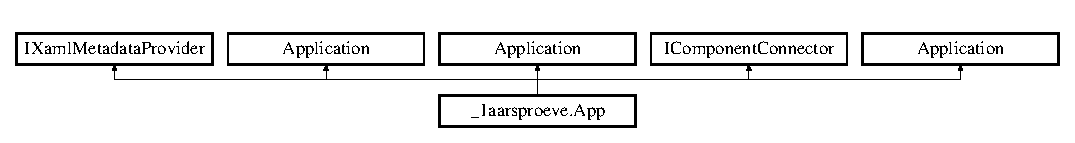
\includegraphics[height=1.473684cm]{class__1aarsproeve_1_1_app}
\end{center}
\end{figure}
\subsection*{Public Member Functions}
\begin{DoxyCompactItemize}
\item 
\hyperlink{class__1aarsproeve_1_1_app_a648545b697c46f7f879d3663198c24df}{App} ()
\begin{DoxyCompactList}\small\item\em Initializes the singleton application object. This is the first line of authored code executed, and as such is the logical equivalent of main() or Win\+Main(). \end{DoxyCompactList}\item 
\hypertarget{class__1aarsproeve_1_1_app_adeff2998728d62ed327627d0ac86916a}{}void {\bfseries Connect} (int connection\+Id, object target)\label{class__1aarsproeve_1_1_app_adeff2998728d62ed327627d0ac86916a}

\item 
\hypertarget{class__1aarsproeve_1_1_app_a3253c2995de585aac3f8db9e63fef8d5}{}void {\bfseries Initialize\+Component} ()\label{class__1aarsproeve_1_1_app_a3253c2995de585aac3f8db9e63fef8d5}

\item 
\hypertarget{class__1aarsproeve_1_1_app_a5114dc7c38ce1d6a07c6cf00fc555545}{}global\+::\+Windows.\+U\+I.\+Xaml.\+Markup.\+I\+Xaml\+Type {\bfseries Get\+Xaml\+Type} (global\+::\+System.\+Type type)\label{class__1aarsproeve_1_1_app_a5114dc7c38ce1d6a07c6cf00fc555545}

\item 
\hypertarget{class__1aarsproeve_1_1_app_a53d51c17fe7ca626f8eb7a25f6c24124}{}global\+::\+Windows.\+U\+I.\+Xaml.\+Markup.\+I\+Xaml\+Type {\bfseries Get\+Xaml\+Type} (string full\+Name)\label{class__1aarsproeve_1_1_app_a53d51c17fe7ca626f8eb7a25f6c24124}

\item 
\hypertarget{class__1aarsproeve_1_1_app_a9d2a8b1a028089c66bd83c91b1cc4528}{}global\+::\+Windows.\+U\+I.\+Xaml.\+Markup.\+Xmlns\+Definition\mbox{[}$\,$\mbox{]} {\bfseries Get\+Xmlns\+Definitions} ()\label{class__1aarsproeve_1_1_app_a9d2a8b1a028089c66bd83c91b1cc4528}

\end{DoxyCompactItemize}
\subsection*{Protected Member Functions}
\begin{DoxyCompactItemize}
\item 
override void \hyperlink{class__1aarsproeve_1_1_app_a1792d58bc636406fca229cf51ac6b81c}{On\+Launched} (Launch\+Activated\+Event\+Args e)
\begin{DoxyCompactList}\small\item\em Invoked when the application is launched normally by the end user. Other entry points will be used such as when the application is launched to open a specific file. \end{DoxyCompactList}\end{DoxyCompactItemize}


\subsection{Detailed Description}
Provides application-\/specific behavior to supplement the default Application class. 



\subsection{Constructor \& Destructor Documentation}
\hypertarget{class__1aarsproeve_1_1_app_a648545b697c46f7f879d3663198c24df}{}\index{\+\_\+1aarsproeve\+::\+App@{\+\_\+1aarsproeve\+::\+App}!App@{App}}
\index{App@{App}!\+\_\+1aarsproeve\+::\+App@{\+\_\+1aarsproeve\+::\+App}}
\subsubsection[{App}]{\setlength{\rightskip}{0pt plus 5cm}\+\_\+1aarsproeve.\+App.\+App (
\begin{DoxyParamCaption}
{}
\end{DoxyParamCaption}
)}\label{class__1aarsproeve_1_1_app_a648545b697c46f7f879d3663198c24df}


Initializes the singleton application object. This is the first line of authored code executed, and as such is the logical equivalent of main() or Win\+Main(). 



\subsection{Member Function Documentation}
\hypertarget{class__1aarsproeve_1_1_app_a1792d58bc636406fca229cf51ac6b81c}{}\index{\+\_\+1aarsproeve\+::\+App@{\+\_\+1aarsproeve\+::\+App}!On\+Launched@{On\+Launched}}
\index{On\+Launched@{On\+Launched}!\+\_\+1aarsproeve\+::\+App@{\+\_\+1aarsproeve\+::\+App}}
\subsubsection[{On\+Launched}]{\setlength{\rightskip}{0pt plus 5cm}override void \+\_\+1aarsproeve.\+App.\+On\+Launched (
\begin{DoxyParamCaption}
\item[{Launch\+Activated\+Event\+Args}]{e}
\end{DoxyParamCaption}
)\hspace{0.3cm}{\ttfamily [protected]}}\label{class__1aarsproeve_1_1_app_a1792d58bc636406fca229cf51ac6b81c}


Invoked when the application is launched normally by the end user. Other entry points will be used such as when the application is launched to open a specific file. 


\begin{DoxyParams}{Parameters}
{\em e} & Details about the launch request and process.\\
\hline
\end{DoxyParams}


The documentation for this class was generated from the following files\+:\begin{DoxyCompactItemize}
\item 
Documents/\+Git\+Hub/1-\/aarsproeve/1aarsproeve/1aarsproeve/App.\+xaml.\+cs\item 
Documents/\+Git\+Hub/1-\/aarsproeve/1aarsproeve/1aarsproeve/obj/\+Debug/App.\+g.\+i.\+cs\item 
Documents/\+Git\+Hub/1-\/aarsproeve/1aarsproeve/1aarsproeve/obj/\+Debug/Xaml\+Type\+Info.\+g.\+cs\item 
Documents/\+Git\+Hub/1-\/aarsproeve/1aarsproeve/1aarsproeve/obj/\+Debug/App.\+g.\+cs\end{DoxyCompactItemize}

\hypertarget{class__1aarsproeve_1_1_view_1_1_basic_page1}{}\section{\+\_\+1aarsproeve.\+View.\+Basic\+Page1 Class Reference}
\label{class__1aarsproeve_1_1_view_1_1_basic_page1}\index{\+\_\+1aarsproeve.\+View.\+Basic\+Page1@{\+\_\+1aarsproeve.\+View.\+Basic\+Page1}}
Inheritance diagram for \+\_\+1aarsproeve.\+View.\+Basic\+Page1\+:\begin{figure}[H]
\begin{center}
\leavevmode
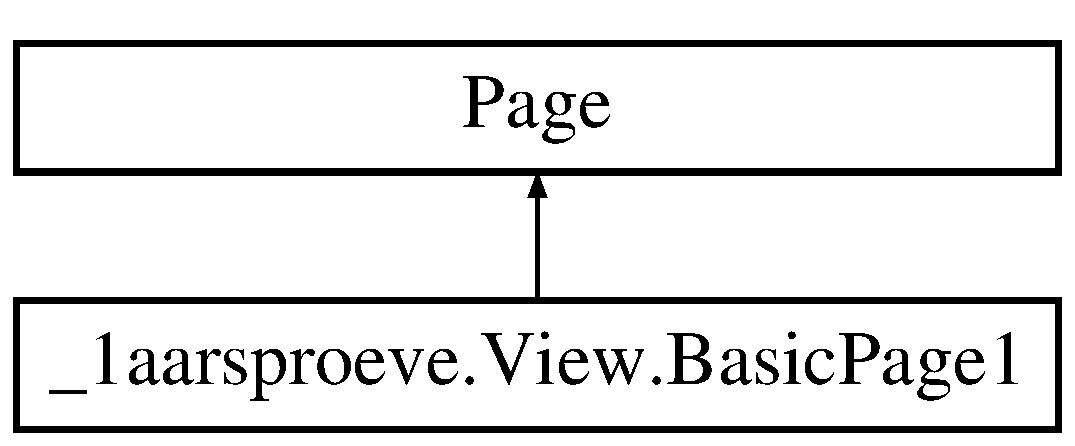
\includegraphics[height=2.000000cm]{class__1aarsproeve_1_1_view_1_1_basic_page1}
\end{center}
\end{figure}
\subsection*{Public Member Functions}
\begin{DoxyCompactItemize}
\item 
\hypertarget{class__1aarsproeve_1_1_view_1_1_basic_page1_a3ab3823b20bab45db7e1c30759ad354e}{}void {\bfseries Initialize\+Component} ()\label{class__1aarsproeve_1_1_view_1_1_basic_page1_a3ab3823b20bab45db7e1c30759ad354e}

\end{DoxyCompactItemize}


The documentation for this class was generated from the following file\+:\begin{DoxyCompactItemize}
\item 
Documents/\+Git\+Hub/1-\/aarsproeve/1aarsproeve/1aarsproeve/obj/\+Debug/\+View/Basic\+Page1.\+g.\+i.\+cs\end{DoxyCompactItemize}

\hypertarget{class__1aarsproeve_1_1_view_model_1_1_bruger_view_model}{}\section{\+\_\+1aarsproeve.\+View\+Model.\+Bruger\+View\+Model Class Reference}
\label{class__1aarsproeve_1_1_view_model_1_1_bruger_view_model}\index{\+\_\+1aarsproeve.\+View\+Model.\+Bruger\+View\+Model@{\+\_\+1aarsproeve.\+View\+Model.\+Bruger\+View\+Model}}
\subsection*{Public Member Functions}
\begin{DoxyCompactItemize}
\item 
\hypertarget{class__1aarsproeve_1_1_view_model_1_1_bruger_view_model_a8c2d6da5fad3a9bdbbde9ce986dcbc74}{}void {\bfseries Log\+Ud} ()\label{class__1aarsproeve_1_1_view_model_1_1_bruger_view_model_a8c2d6da5fad3a9bdbbde9ce986dcbc74}

\end{DoxyCompactItemize}
\subsection*{Properties}
\begin{DoxyCompactItemize}
\item 
\hypertarget{class__1aarsproeve_1_1_view_model_1_1_bruger_view_model_ac9e91065596a741027a1b88853bd76e6}{}Application\+Data\+Container {\bfseries Setting}\hspace{0.3cm}{\ttfamily  \mbox{[}get, set\mbox{]}}\label{class__1aarsproeve_1_1_view_model_1_1_bruger_view_model_ac9e91065596a741027a1b88853bd76e6}

\item 
\hypertarget{class__1aarsproeve_1_1_view_model_1_1_bruger_view_model_a63b4a8aa59a8e3e2ec0d7285c2ce6caa}{}string {\bfseries Brugernavn}\hspace{0.3cm}{\ttfamily  \mbox{[}get, set\mbox{]}}\label{class__1aarsproeve_1_1_view_model_1_1_bruger_view_model_a63b4a8aa59a8e3e2ec0d7285c2ce6caa}

\item 
\hypertarget{class__1aarsproeve_1_1_view_model_1_1_bruger_view_model_a40fed761861b9387bc47a92a2f1e55fd}{}I\+Command {\bfseries Log\+Ind\+Command}\hspace{0.3cm}{\ttfamily  \mbox{[}get, set\mbox{]}}\label{class__1aarsproeve_1_1_view_model_1_1_bruger_view_model_a40fed761861b9387bc47a92a2f1e55fd}

\item 
\hypertarget{class__1aarsproeve_1_1_view_model_1_1_bruger_view_model_afc1d332a62edcc717d3e1764db42c89a}{}I\+Command {\bfseries Log\+Ud\+Command}\hspace{0.3cm}{\ttfamily  \mbox{[}get, set\mbox{]}}\label{class__1aarsproeve_1_1_view_model_1_1_bruger_view_model_afc1d332a62edcc717d3e1764db42c89a}

\end{DoxyCompactItemize}


The documentation for this class was generated from the following file\+:\begin{DoxyCompactItemize}
\item 
C\+:/\+Users/\+Daniel\+Winther/\+Documents/\+Git\+Hub/1-\/aarsproeve/1aarsproeve/1aarsproeve/\+View\+Model/Bruger\+View\+Model.\+cs\end{DoxyCompactItemize}

\hypertarget{class__1aarsproeve_web_service_1_1_bundle_config}{}\section{\+\_\+1aarsproeve\+Web\+Service.\+Bundle\+Config Class Reference}
\label{class__1aarsproeve_web_service_1_1_bundle_config}\index{\+\_\+1aarsproeve\+Web\+Service.\+Bundle\+Config@{\+\_\+1aarsproeve\+Web\+Service.\+Bundle\+Config}}
\subsection*{Static Public Member Functions}
\begin{DoxyCompactItemize}
\item 
\hypertarget{class__1aarsproeve_web_service_1_1_bundle_config_ab9a18fe210fb037e3bdb7405a0b456e6}{}static void {\bfseries Register\+Bundles} (Bundle\+Collection bundles)\label{class__1aarsproeve_web_service_1_1_bundle_config_ab9a18fe210fb037e3bdb7405a0b456e6}

\end{DoxyCompactItemize}


The documentation for this class was generated from the following file\+:\begin{DoxyCompactItemize}
\item 
C\+:/\+Users/\+Daniel\+Winther/\+Documents/\+Git\+Hub/1-\/aarsproeve/1aarsproeve/1aarsproeve\+Web\+Service/\+App\+\_\+\+Start/Bundle\+Config.\+cs\end{DoxyCompactItemize}

\hypertarget{class__1aarsproeve_web_service_1_1_areas_1_1_help_page_1_1_model_descriptions_1_1_collection_model_description}{}\section{\+\_\+1aarsproeve\+Web\+Service.\+Areas.\+Help\+Page.\+Model\+Descriptions.\+Collection\+Model\+Description Class Reference}
\label{class__1aarsproeve_web_service_1_1_areas_1_1_help_page_1_1_model_descriptions_1_1_collection_model_description}\index{\+\_\+1aarsproeve\+Web\+Service.\+Areas.\+Help\+Page.\+Model\+Descriptions.\+Collection\+Model\+Description@{\+\_\+1aarsproeve\+Web\+Service.\+Areas.\+Help\+Page.\+Model\+Descriptions.\+Collection\+Model\+Description}}
Inheritance diagram for \+\_\+1aarsproeve\+Web\+Service.\+Areas.\+Help\+Page.\+Model\+Descriptions.\+Collection\+Model\+Description\+:\begin{figure}[H]
\begin{center}
\leavevmode
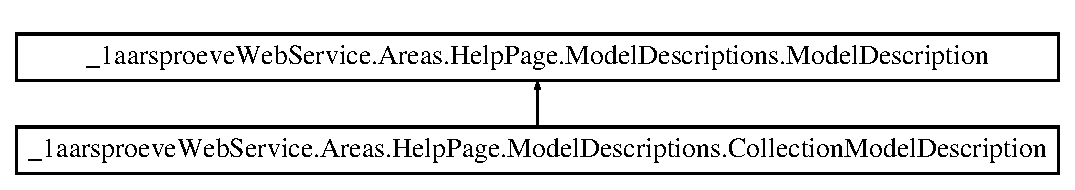
\includegraphics[height=2.000000cm]{class__1aarsproeve_web_service_1_1_areas_1_1_help_page_1_1_model_descriptions_1_1_collection_model_description}
\end{center}
\end{figure}
\subsection*{Properties}
\begin{DoxyCompactItemize}
\item 
\hypertarget{class__1aarsproeve_web_service_1_1_areas_1_1_help_page_1_1_model_descriptions_1_1_collection_model_description_a9f59a1485146c386bb767ff88380e3b2}{}\hyperlink{class__1aarsproeve_web_service_1_1_areas_1_1_help_page_1_1_model_descriptions_1_1_model_description}{Model\+Description} {\bfseries Element\+Description}\hspace{0.3cm}{\ttfamily  \mbox{[}get, set\mbox{]}}\label{class__1aarsproeve_web_service_1_1_areas_1_1_help_page_1_1_model_descriptions_1_1_collection_model_description_a9f59a1485146c386bb767ff88380e3b2}

\end{DoxyCompactItemize}


The documentation for this class was generated from the following file\+:\begin{DoxyCompactItemize}
\item 
Documents/\+Git\+Hub/1-\/aarsproeve/1aarsproeve/1aarsproeve\+Web\+Service/\+Areas/\+Help\+Page/\+Model\+Descriptions/Collection\+Model\+Description.\+cs\end{DoxyCompactItemize}

\hypertarget{class__1aarsproeve_web_service_1_1_areas_1_1_help_page_1_1_model_descriptions_1_1_complex_type_model_description}{}\section{\+\_\+1aarsproeve\+Web\+Service.\+Areas.\+Help\+Page.\+Model\+Descriptions.\+Complex\+Type\+Model\+Description Class Reference}
\label{class__1aarsproeve_web_service_1_1_areas_1_1_help_page_1_1_model_descriptions_1_1_complex_type_model_description}\index{\+\_\+1aarsproeve\+Web\+Service.\+Areas.\+Help\+Page.\+Model\+Descriptions.\+Complex\+Type\+Model\+Description@{\+\_\+1aarsproeve\+Web\+Service.\+Areas.\+Help\+Page.\+Model\+Descriptions.\+Complex\+Type\+Model\+Description}}
Inheritance diagram for \+\_\+1aarsproeve\+Web\+Service.\+Areas.\+Help\+Page.\+Model\+Descriptions.\+Complex\+Type\+Model\+Description\+:\begin{figure}[H]
\begin{center}
\leavevmode
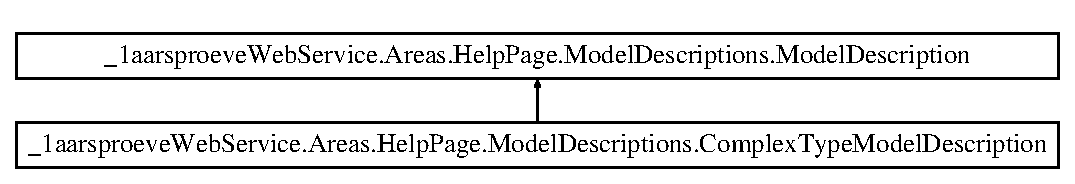
\includegraphics[height=2.000000cm]{class__1aarsproeve_web_service_1_1_areas_1_1_help_page_1_1_model_descriptions_1_1_complex_type_model_description}
\end{center}
\end{figure}
\subsection*{Properties}
\begin{DoxyCompactItemize}
\item 
\hypertarget{class__1aarsproeve_web_service_1_1_areas_1_1_help_page_1_1_model_descriptions_1_1_complex_type_model_description_afabdec8e2987c716ec40a6d32410fca9}{}Collection$<$ \hyperlink{class__1aarsproeve_web_service_1_1_areas_1_1_help_page_1_1_model_descriptions_1_1_parameter_description}{Parameter\+Description} $>$ {\bfseries Properties}\hspace{0.3cm}{\ttfamily  \mbox{[}get\mbox{]}}\label{class__1aarsproeve_web_service_1_1_areas_1_1_help_page_1_1_model_descriptions_1_1_complex_type_model_description_afabdec8e2987c716ec40a6d32410fca9}

\end{DoxyCompactItemize}


The documentation for this class was generated from the following file\+:\begin{DoxyCompactItemize}
\item 
C\+:/\+Users/\+Daniel\+Winther/\+Documents/\+Git\+Hub/1-\/aarsproeve/1aarsproeve/1aarsproeve\+Web\+Service/\+Areas/\+Help\+Page/\+Model\+Descriptions/Complex\+Type\+Model\+Description.\+cs\end{DoxyCompactItemize}

\hypertarget{class__1aarsproeve_web_service_1_1_areas_1_1_help_page_1_1_model_descriptions_1_1_dictionary_model_description}{}\section{\+\_\+1aarsproeve\+Web\+Service.\+Areas.\+Help\+Page.\+Model\+Descriptions.\+Dictionary\+Model\+Description Class Reference}
\label{class__1aarsproeve_web_service_1_1_areas_1_1_help_page_1_1_model_descriptions_1_1_dictionary_model_description}\index{\+\_\+1aarsproeve\+Web\+Service.\+Areas.\+Help\+Page.\+Model\+Descriptions.\+Dictionary\+Model\+Description@{\+\_\+1aarsproeve\+Web\+Service.\+Areas.\+Help\+Page.\+Model\+Descriptions.\+Dictionary\+Model\+Description}}
Inheritance diagram for \+\_\+1aarsproeve\+Web\+Service.\+Areas.\+Help\+Page.\+Model\+Descriptions.\+Dictionary\+Model\+Description\+:\begin{figure}[H]
\begin{center}
\leavevmode
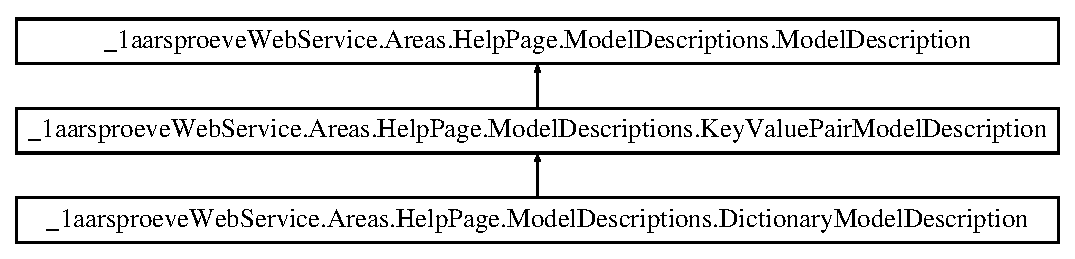
\includegraphics[height=3.000000cm]{class__1aarsproeve_web_service_1_1_areas_1_1_help_page_1_1_model_descriptions_1_1_dictionary_model_description}
\end{center}
\end{figure}
\subsection*{Additional Inherited Members}


The documentation for this class was generated from the following file\+:\begin{DoxyCompactItemize}
\item 
C\+:/\+Users/\+Daniel\+Winther/\+Documents/\+Git\+Hub/1-\/aarsproeve/1aarsproeve/1aarsproeve\+Web\+Service/\+Areas/\+Help\+Page/\+Model\+Descriptions/Dictionary\+Model\+Description.\+cs\end{DoxyCompactItemize}

\hypertarget{class__1aarsproeve_web_service_1_1_areas_1_1_help_page_1_1_model_descriptions_1_1_enum_type_model_description}{}\section{\+\_\+1aarsproeve\+Web\+Service.\+Areas.\+Help\+Page.\+Model\+Descriptions.\+Enum\+Type\+Model\+Description Class Reference}
\label{class__1aarsproeve_web_service_1_1_areas_1_1_help_page_1_1_model_descriptions_1_1_enum_type_model_description}\index{\+\_\+1aarsproeve\+Web\+Service.\+Areas.\+Help\+Page.\+Model\+Descriptions.\+Enum\+Type\+Model\+Description@{\+\_\+1aarsproeve\+Web\+Service.\+Areas.\+Help\+Page.\+Model\+Descriptions.\+Enum\+Type\+Model\+Description}}
Inheritance diagram for \+\_\+1aarsproeve\+Web\+Service.\+Areas.\+Help\+Page.\+Model\+Descriptions.\+Enum\+Type\+Model\+Description\+:\begin{figure}[H]
\begin{center}
\leavevmode
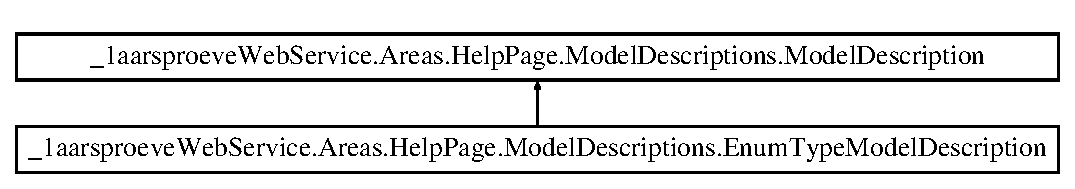
\includegraphics[height=2.000000cm]{class__1aarsproeve_web_service_1_1_areas_1_1_help_page_1_1_model_descriptions_1_1_enum_type_model_description}
\end{center}
\end{figure}
\subsection*{Properties}
\begin{DoxyCompactItemize}
\item 
\hypertarget{class__1aarsproeve_web_service_1_1_areas_1_1_help_page_1_1_model_descriptions_1_1_enum_type_model_description_a0d1a08eead95b9223e53b77770bc8703}{}Collection$<$ \hyperlink{class__1aarsproeve_web_service_1_1_areas_1_1_help_page_1_1_model_descriptions_1_1_enum_value_description}{Enum\+Value\+Description} $>$ {\bfseries Values}\hspace{0.3cm}{\ttfamily  \mbox{[}get\mbox{]}}\label{class__1aarsproeve_web_service_1_1_areas_1_1_help_page_1_1_model_descriptions_1_1_enum_type_model_description_a0d1a08eead95b9223e53b77770bc8703}

\end{DoxyCompactItemize}


The documentation for this class was generated from the following file\+:\begin{DoxyCompactItemize}
\item 
C\+:/\+Users/\+Daniel\+Winther/\+Documents/\+Git\+Hub/1-\/aarsproeve/1aarsproeve/1aarsproeve\+Web\+Service/\+Areas/\+Help\+Page/\+Model\+Descriptions/Enum\+Type\+Model\+Description.\+cs\end{DoxyCompactItemize}

\hypertarget{class__1aarsproeve_web_service_1_1_areas_1_1_help_page_1_1_model_descriptions_1_1_enum_value_description}{}\section{\+\_\+1aarsproeve\+Web\+Service.\+Areas.\+Help\+Page.\+Model\+Descriptions.\+Enum\+Value\+Description Class Reference}
\label{class__1aarsproeve_web_service_1_1_areas_1_1_help_page_1_1_model_descriptions_1_1_enum_value_description}\index{\+\_\+1aarsproeve\+Web\+Service.\+Areas.\+Help\+Page.\+Model\+Descriptions.\+Enum\+Value\+Description@{\+\_\+1aarsproeve\+Web\+Service.\+Areas.\+Help\+Page.\+Model\+Descriptions.\+Enum\+Value\+Description}}
\subsection*{Properties}
\begin{DoxyCompactItemize}
\item 
\hypertarget{class__1aarsproeve_web_service_1_1_areas_1_1_help_page_1_1_model_descriptions_1_1_enum_value_description_a8b2b1e0baf970953a104b1c468a68c61}{}string {\bfseries Documentation}\hspace{0.3cm}{\ttfamily  \mbox{[}get, set\mbox{]}}\label{class__1aarsproeve_web_service_1_1_areas_1_1_help_page_1_1_model_descriptions_1_1_enum_value_description_a8b2b1e0baf970953a104b1c468a68c61}

\item 
\hypertarget{class__1aarsproeve_web_service_1_1_areas_1_1_help_page_1_1_model_descriptions_1_1_enum_value_description_a7d3d2652afe86ecef65fa066bd7a233b}{}string {\bfseries Name}\hspace{0.3cm}{\ttfamily  \mbox{[}get, set\mbox{]}}\label{class__1aarsproeve_web_service_1_1_areas_1_1_help_page_1_1_model_descriptions_1_1_enum_value_description_a7d3d2652afe86ecef65fa066bd7a233b}

\item 
\hypertarget{class__1aarsproeve_web_service_1_1_areas_1_1_help_page_1_1_model_descriptions_1_1_enum_value_description_a0670b18ee3d0ffe91340b5bc62e1b21a}{}string {\bfseries Value}\hspace{0.3cm}{\ttfamily  \mbox{[}get, set\mbox{]}}\label{class__1aarsproeve_web_service_1_1_areas_1_1_help_page_1_1_model_descriptions_1_1_enum_value_description_a0670b18ee3d0ffe91340b5bc62e1b21a}

\end{DoxyCompactItemize}


The documentation for this class was generated from the following file\+:\begin{DoxyCompactItemize}
\item 
Documents/\+Git\+Hub/1-\/aarsproeve/1aarsproeve/1aarsproeve\+Web\+Service/\+Areas/\+Help\+Page/\+Model\+Descriptions/Enum\+Value\+Description.\+cs\end{DoxyCompactItemize}

\hypertarget{class__1aarsproeve_web_service_1_1_filter_config}{}\section{\+\_\+1aarsproeve\+Web\+Service.\+Filter\+Config Class Reference}
\label{class__1aarsproeve_web_service_1_1_filter_config}\index{\+\_\+1aarsproeve\+Web\+Service.\+Filter\+Config@{\+\_\+1aarsproeve\+Web\+Service.\+Filter\+Config}}
\subsection*{Static Public Member Functions}
\begin{DoxyCompactItemize}
\item 
\hypertarget{class__1aarsproeve_web_service_1_1_filter_config_aa408c602cd6d9244e1299d9c2ab9566e}{}static void {\bfseries Register\+Global\+Filters} (Global\+Filter\+Collection filters)\label{class__1aarsproeve_web_service_1_1_filter_config_aa408c602cd6d9244e1299d9c2ab9566e}

\end{DoxyCompactItemize}


The documentation for this class was generated from the following file\+:\begin{DoxyCompactItemize}
\item 
Documents/\+Git\+Hub/1-\/aarsproeve/1aarsproeve/1aarsproeve\+Web\+Service/\+App\+\_\+\+Start/Filter\+Config.\+cs\end{DoxyCompactItemize}

\hypertarget{class__1aarsproeve_web_service_1_1_areas_1_1_help_page_1_1_controllers_1_1_help_controller}{}\section{\+\_\+1aarsproeve\+Web\+Service.\+Areas.\+Help\+Page.\+Controllers.\+Help\+Controller Class Reference}
\label{class__1aarsproeve_web_service_1_1_areas_1_1_help_page_1_1_controllers_1_1_help_controller}\index{\+\_\+1aarsproeve\+Web\+Service.\+Areas.\+Help\+Page.\+Controllers.\+Help\+Controller@{\+\_\+1aarsproeve\+Web\+Service.\+Areas.\+Help\+Page.\+Controllers.\+Help\+Controller}}


The controller that will handle requests for the help page.  


Inheritance diagram for \+\_\+1aarsproeve\+Web\+Service.\+Areas.\+Help\+Page.\+Controllers.\+Help\+Controller\+:\begin{figure}[H]
\begin{center}
\leavevmode
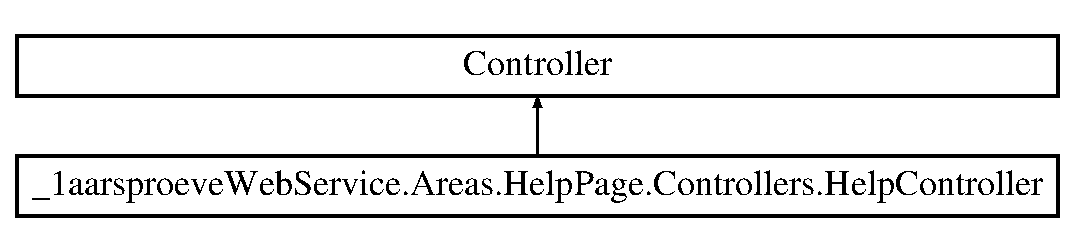
\includegraphics[height=2.000000cm]{class__1aarsproeve_web_service_1_1_areas_1_1_help_page_1_1_controllers_1_1_help_controller}
\end{center}
\end{figure}
\subsection*{Public Member Functions}
\begin{DoxyCompactItemize}
\item 
\hypertarget{class__1aarsproeve_web_service_1_1_areas_1_1_help_page_1_1_controllers_1_1_help_controller_ac5863469ead4f269ca923864b1b000bb}{}{\bfseries Help\+Controller} (Http\+Configuration config)\label{class__1aarsproeve_web_service_1_1_areas_1_1_help_page_1_1_controllers_1_1_help_controller_ac5863469ead4f269ca923864b1b000bb}

\item 
\hypertarget{class__1aarsproeve_web_service_1_1_areas_1_1_help_page_1_1_controllers_1_1_help_controller_ac8ab14f8de06e3b728040556b86976bb}{}Action\+Result {\bfseries Index} ()\label{class__1aarsproeve_web_service_1_1_areas_1_1_help_page_1_1_controllers_1_1_help_controller_ac8ab14f8de06e3b728040556b86976bb}

\item 
\hypertarget{class__1aarsproeve_web_service_1_1_areas_1_1_help_page_1_1_controllers_1_1_help_controller_aedb2d9f385044bd702dde25cd83ef505}{}Action\+Result {\bfseries Api} (string api\+Id)\label{class__1aarsproeve_web_service_1_1_areas_1_1_help_page_1_1_controllers_1_1_help_controller_aedb2d9f385044bd702dde25cd83ef505}

\item 
\hypertarget{class__1aarsproeve_web_service_1_1_areas_1_1_help_page_1_1_controllers_1_1_help_controller_a0d6027c97d0dfaf55e3399a8ec8625b7}{}Action\+Result {\bfseries Resource\+Model} (string model\+Name)\label{class__1aarsproeve_web_service_1_1_areas_1_1_help_page_1_1_controllers_1_1_help_controller_a0d6027c97d0dfaf55e3399a8ec8625b7}

\end{DoxyCompactItemize}
\subsection*{Properties}
\begin{DoxyCompactItemize}
\item 
\hypertarget{class__1aarsproeve_web_service_1_1_areas_1_1_help_page_1_1_controllers_1_1_help_controller_ae617e8e48348cf6dd582b758ee6cef66}{}Http\+Configuration {\bfseries Configuration}\hspace{0.3cm}{\ttfamily  \mbox{[}get\mbox{]}}\label{class__1aarsproeve_web_service_1_1_areas_1_1_help_page_1_1_controllers_1_1_help_controller_ae617e8e48348cf6dd582b758ee6cef66}

\end{DoxyCompactItemize}


\subsection{Detailed Description}
The controller that will handle requests for the help page. 



The documentation for this class was generated from the following file\+:\begin{DoxyCompactItemize}
\item 
C\+:/\+Users/\+Daniel\+Winther/\+Documents/\+Git\+Hub/1-\/aarsproeve/1aarsproeve/1aarsproeve\+Web\+Service/\+Areas/\+Help\+Page/\+Controllers/Help\+Controller.\+cs\end{DoxyCompactItemize}

\hypertarget{class__1aarsproeve_web_service_1_1_areas_1_1_help_page_1_1_models_1_1_help_page_api_model}{}\section{\+\_\+1aarsproeve\+Web\+Service.\+Areas.\+Help\+Page.\+Models.\+Help\+Page\+Api\+Model Class Reference}
\label{class__1aarsproeve_web_service_1_1_areas_1_1_help_page_1_1_models_1_1_help_page_api_model}\index{\+\_\+1aarsproeve\+Web\+Service.\+Areas.\+Help\+Page.\+Models.\+Help\+Page\+Api\+Model@{\+\_\+1aarsproeve\+Web\+Service.\+Areas.\+Help\+Page.\+Models.\+Help\+Page\+Api\+Model}}


The model that represents an A\+P\+I displayed on the help page.  


\subsection*{Public Member Functions}
\begin{DoxyCompactItemize}
\item 
\hyperlink{class__1aarsproeve_web_service_1_1_areas_1_1_help_page_1_1_models_1_1_help_page_api_model_aea81d3b4b0294cd9753efb03c91bf2eb}{Help\+Page\+Api\+Model} ()
\begin{DoxyCompactList}\small\item\em Initializes a new instance of the \hyperlink{class__1aarsproeve_web_service_1_1_areas_1_1_help_page_1_1_models_1_1_help_page_api_model}{Help\+Page\+Api\+Model} class. \end{DoxyCompactList}\end{DoxyCompactItemize}
\subsection*{Properties}
\begin{DoxyCompactItemize}
\item 
Api\+Description \hyperlink{class__1aarsproeve_web_service_1_1_areas_1_1_help_page_1_1_models_1_1_help_page_api_model_a8b1d233d46646da325139313fe77cedc}{Api\+Description}\hspace{0.3cm}{\ttfamily  \mbox{[}get, set\mbox{]}}
\begin{DoxyCompactList}\small\item\em Gets or sets the \hyperlink{class__1aarsproeve_web_service_1_1_areas_1_1_help_page_1_1_models_1_1_help_page_api_model_a8b1d233d46646da325139313fe77cedc}{Api\+Description} that describes the A\+P\+I. \end{DoxyCompactList}\item 
Collection$<$ \hyperlink{class__1aarsproeve_web_service_1_1_areas_1_1_help_page_1_1_model_descriptions_1_1_parameter_description}{Parameter\+Description} $>$ \hyperlink{class__1aarsproeve_web_service_1_1_areas_1_1_help_page_1_1_models_1_1_help_page_api_model_a13910e263edc19222bbb60615d1f80be}{Uri\+Parameters}\hspace{0.3cm}{\ttfamily  \mbox{[}get\mbox{]}}
\begin{DoxyCompactList}\small\item\em Gets or sets the Parameter\+Description collection that describes the U\+R\+I parameters for the A\+P\+I. \end{DoxyCompactList}\item 
string \hyperlink{class__1aarsproeve_web_service_1_1_areas_1_1_help_page_1_1_models_1_1_help_page_api_model_a7c6ab7ddf1586125e6de402d850fddab}{Request\+Documentation}\hspace{0.3cm}{\ttfamily  \mbox{[}get, set\mbox{]}}
\begin{DoxyCompactList}\small\item\em Gets or sets the documentation for the request. \end{DoxyCompactList}\item 
\hyperlink{class__1aarsproeve_web_service_1_1_areas_1_1_help_page_1_1_model_descriptions_1_1_model_description}{Model\+Description} \hyperlink{class__1aarsproeve_web_service_1_1_areas_1_1_help_page_1_1_models_1_1_help_page_api_model_ab70ab5430b41f8c40c1ff4bb5aec3eca}{Request\+Model\+Description}\hspace{0.3cm}{\ttfamily  \mbox{[}get, set\mbox{]}}
\begin{DoxyCompactList}\small\item\em Gets or sets the Model\+Description that describes the request body. \end{DoxyCompactList}\item 
I\+List$<$ \hyperlink{class__1aarsproeve_web_service_1_1_areas_1_1_help_page_1_1_model_descriptions_1_1_parameter_description}{Parameter\+Description} $>$ \hyperlink{class__1aarsproeve_web_service_1_1_areas_1_1_help_page_1_1_models_1_1_help_page_api_model_a01d824c4a2e89f5c4464fc1a077361a6}{Request\+Body\+Parameters}\hspace{0.3cm}{\ttfamily  \mbox{[}get\mbox{]}}
\begin{DoxyCompactList}\small\item\em Gets the request body parameter descriptions. \end{DoxyCompactList}\item 
\hyperlink{class__1aarsproeve_web_service_1_1_areas_1_1_help_page_1_1_model_descriptions_1_1_model_description}{Model\+Description} \hyperlink{class__1aarsproeve_web_service_1_1_areas_1_1_help_page_1_1_models_1_1_help_page_api_model_a190780aa4262f4e6da85944b57e57307}{Resource\+Description}\hspace{0.3cm}{\ttfamily  \mbox{[}get, set\mbox{]}}
\begin{DoxyCompactList}\small\item\em Gets or sets the Model\+Description that describes the resource. \end{DoxyCompactList}\item 
I\+List$<$ \hyperlink{class__1aarsproeve_web_service_1_1_areas_1_1_help_page_1_1_model_descriptions_1_1_parameter_description}{Parameter\+Description} $>$ \hyperlink{class__1aarsproeve_web_service_1_1_areas_1_1_help_page_1_1_models_1_1_help_page_api_model_a9ab05000ce11c2ab4d69f190f2177239}{Resource\+Properties}\hspace{0.3cm}{\ttfamily  \mbox{[}get\mbox{]}}
\begin{DoxyCompactList}\small\item\em Gets the resource property descriptions. \end{DoxyCompactList}\item 
I\+Dictionary$<$ Media\+Type\+Header\+Value, object $>$ \hyperlink{class__1aarsproeve_web_service_1_1_areas_1_1_help_page_1_1_models_1_1_help_page_api_model_a28948b3477b00b650df4df27d9a1b866}{Sample\+Requests}\hspace{0.3cm}{\ttfamily  \mbox{[}get\mbox{]}}
\begin{DoxyCompactList}\small\item\em Gets the sample requests associated with the A\+P\+I. \end{DoxyCompactList}\item 
I\+Dictionary$<$ Media\+Type\+Header\+Value, object $>$ \hyperlink{class__1aarsproeve_web_service_1_1_areas_1_1_help_page_1_1_models_1_1_help_page_api_model_aa2176c7fd5b4e47329d2cecee146fdaa}{Sample\+Responses}\hspace{0.3cm}{\ttfamily  \mbox{[}get\mbox{]}}
\begin{DoxyCompactList}\small\item\em Gets the sample responses associated with the A\+P\+I. \end{DoxyCompactList}\item 
Collection$<$ string $>$ \hyperlink{class__1aarsproeve_web_service_1_1_areas_1_1_help_page_1_1_models_1_1_help_page_api_model_a89a4a8ab5f162a7feca59255edef5e50}{Error\+Messages}\hspace{0.3cm}{\ttfamily  \mbox{[}get\mbox{]}}
\begin{DoxyCompactList}\small\item\em Gets the error messages associated with this model. \end{DoxyCompactList}\end{DoxyCompactItemize}


\subsection{Detailed Description}
The model that represents an A\+P\+I displayed on the help page. 



\subsection{Constructor \& Destructor Documentation}
\hypertarget{class__1aarsproeve_web_service_1_1_areas_1_1_help_page_1_1_models_1_1_help_page_api_model_aea81d3b4b0294cd9753efb03c91bf2eb}{}\index{\+\_\+1aarsproeve\+Web\+Service\+::\+Areas\+::\+Help\+Page\+::\+Models\+::\+Help\+Page\+Api\+Model@{\+\_\+1aarsproeve\+Web\+Service\+::\+Areas\+::\+Help\+Page\+::\+Models\+::\+Help\+Page\+Api\+Model}!Help\+Page\+Api\+Model@{Help\+Page\+Api\+Model}}
\index{Help\+Page\+Api\+Model@{Help\+Page\+Api\+Model}!\+\_\+1aarsproeve\+Web\+Service\+::\+Areas\+::\+Help\+Page\+::\+Models\+::\+Help\+Page\+Api\+Model@{\+\_\+1aarsproeve\+Web\+Service\+::\+Areas\+::\+Help\+Page\+::\+Models\+::\+Help\+Page\+Api\+Model}}
\subsubsection[{Help\+Page\+Api\+Model}]{\setlength{\rightskip}{0pt plus 5cm}\+\_\+1aarsproeve\+Web\+Service.\+Areas.\+Help\+Page.\+Models.\+Help\+Page\+Api\+Model.\+Help\+Page\+Api\+Model (
\begin{DoxyParamCaption}
{}
\end{DoxyParamCaption}
)\hspace{0.3cm}{\ttfamily [inline]}}\label{class__1aarsproeve_web_service_1_1_areas_1_1_help_page_1_1_models_1_1_help_page_api_model_aea81d3b4b0294cd9753efb03c91bf2eb}


Initializes a new instance of the \hyperlink{class__1aarsproeve_web_service_1_1_areas_1_1_help_page_1_1_models_1_1_help_page_api_model}{Help\+Page\+Api\+Model} class. 



\subsection{Property Documentation}
\hypertarget{class__1aarsproeve_web_service_1_1_areas_1_1_help_page_1_1_models_1_1_help_page_api_model_a8b1d233d46646da325139313fe77cedc}{}\index{\+\_\+1aarsproeve\+Web\+Service\+::\+Areas\+::\+Help\+Page\+::\+Models\+::\+Help\+Page\+Api\+Model@{\+\_\+1aarsproeve\+Web\+Service\+::\+Areas\+::\+Help\+Page\+::\+Models\+::\+Help\+Page\+Api\+Model}!Api\+Description@{Api\+Description}}
\index{Api\+Description@{Api\+Description}!\+\_\+1aarsproeve\+Web\+Service\+::\+Areas\+::\+Help\+Page\+::\+Models\+::\+Help\+Page\+Api\+Model@{\+\_\+1aarsproeve\+Web\+Service\+::\+Areas\+::\+Help\+Page\+::\+Models\+::\+Help\+Page\+Api\+Model}}
\subsubsection[{Api\+Description}]{\setlength{\rightskip}{0pt plus 5cm}Api\+Description \+\_\+1aarsproeve\+Web\+Service.\+Areas.\+Help\+Page.\+Models.\+Help\+Page\+Api\+Model.\+Api\+Description\hspace{0.3cm}{\ttfamily [get]}, {\ttfamily [set]}}\label{class__1aarsproeve_web_service_1_1_areas_1_1_help_page_1_1_models_1_1_help_page_api_model_a8b1d233d46646da325139313fe77cedc}


Gets or sets the \hyperlink{class__1aarsproeve_web_service_1_1_areas_1_1_help_page_1_1_models_1_1_help_page_api_model_a8b1d233d46646da325139313fe77cedc}{Api\+Description} that describes the A\+P\+I. 

\hypertarget{class__1aarsproeve_web_service_1_1_areas_1_1_help_page_1_1_models_1_1_help_page_api_model_a89a4a8ab5f162a7feca59255edef5e50}{}\index{\+\_\+1aarsproeve\+Web\+Service\+::\+Areas\+::\+Help\+Page\+::\+Models\+::\+Help\+Page\+Api\+Model@{\+\_\+1aarsproeve\+Web\+Service\+::\+Areas\+::\+Help\+Page\+::\+Models\+::\+Help\+Page\+Api\+Model}!Error\+Messages@{Error\+Messages}}
\index{Error\+Messages@{Error\+Messages}!\+\_\+1aarsproeve\+Web\+Service\+::\+Areas\+::\+Help\+Page\+::\+Models\+::\+Help\+Page\+Api\+Model@{\+\_\+1aarsproeve\+Web\+Service\+::\+Areas\+::\+Help\+Page\+::\+Models\+::\+Help\+Page\+Api\+Model}}
\subsubsection[{Error\+Messages}]{\setlength{\rightskip}{0pt plus 5cm}Collection$<$string$>$ \+\_\+1aarsproeve\+Web\+Service.\+Areas.\+Help\+Page.\+Models.\+Help\+Page\+Api\+Model.\+Error\+Messages\hspace{0.3cm}{\ttfamily [get]}}\label{class__1aarsproeve_web_service_1_1_areas_1_1_help_page_1_1_models_1_1_help_page_api_model_a89a4a8ab5f162a7feca59255edef5e50}


Gets the error messages associated with this model. 

\hypertarget{class__1aarsproeve_web_service_1_1_areas_1_1_help_page_1_1_models_1_1_help_page_api_model_a01d824c4a2e89f5c4464fc1a077361a6}{}\index{\+\_\+1aarsproeve\+Web\+Service\+::\+Areas\+::\+Help\+Page\+::\+Models\+::\+Help\+Page\+Api\+Model@{\+\_\+1aarsproeve\+Web\+Service\+::\+Areas\+::\+Help\+Page\+::\+Models\+::\+Help\+Page\+Api\+Model}!Request\+Body\+Parameters@{Request\+Body\+Parameters}}
\index{Request\+Body\+Parameters@{Request\+Body\+Parameters}!\+\_\+1aarsproeve\+Web\+Service\+::\+Areas\+::\+Help\+Page\+::\+Models\+::\+Help\+Page\+Api\+Model@{\+\_\+1aarsproeve\+Web\+Service\+::\+Areas\+::\+Help\+Page\+::\+Models\+::\+Help\+Page\+Api\+Model}}
\subsubsection[{Request\+Body\+Parameters}]{\setlength{\rightskip}{0pt plus 5cm}I\+List$<${\bf Parameter\+Description}$>$ \+\_\+1aarsproeve\+Web\+Service.\+Areas.\+Help\+Page.\+Models.\+Help\+Page\+Api\+Model.\+Request\+Body\+Parameters\hspace{0.3cm}{\ttfamily [get]}}\label{class__1aarsproeve_web_service_1_1_areas_1_1_help_page_1_1_models_1_1_help_page_api_model_a01d824c4a2e89f5c4464fc1a077361a6}


Gets the request body parameter descriptions. 

\hypertarget{class__1aarsproeve_web_service_1_1_areas_1_1_help_page_1_1_models_1_1_help_page_api_model_a7c6ab7ddf1586125e6de402d850fddab}{}\index{\+\_\+1aarsproeve\+Web\+Service\+::\+Areas\+::\+Help\+Page\+::\+Models\+::\+Help\+Page\+Api\+Model@{\+\_\+1aarsproeve\+Web\+Service\+::\+Areas\+::\+Help\+Page\+::\+Models\+::\+Help\+Page\+Api\+Model}!Request\+Documentation@{Request\+Documentation}}
\index{Request\+Documentation@{Request\+Documentation}!\+\_\+1aarsproeve\+Web\+Service\+::\+Areas\+::\+Help\+Page\+::\+Models\+::\+Help\+Page\+Api\+Model@{\+\_\+1aarsproeve\+Web\+Service\+::\+Areas\+::\+Help\+Page\+::\+Models\+::\+Help\+Page\+Api\+Model}}
\subsubsection[{Request\+Documentation}]{\setlength{\rightskip}{0pt plus 5cm}string \+\_\+1aarsproeve\+Web\+Service.\+Areas.\+Help\+Page.\+Models.\+Help\+Page\+Api\+Model.\+Request\+Documentation\hspace{0.3cm}{\ttfamily [get]}, {\ttfamily [set]}}\label{class__1aarsproeve_web_service_1_1_areas_1_1_help_page_1_1_models_1_1_help_page_api_model_a7c6ab7ddf1586125e6de402d850fddab}


Gets or sets the documentation for the request. 

\hypertarget{class__1aarsproeve_web_service_1_1_areas_1_1_help_page_1_1_models_1_1_help_page_api_model_ab70ab5430b41f8c40c1ff4bb5aec3eca}{}\index{\+\_\+1aarsproeve\+Web\+Service\+::\+Areas\+::\+Help\+Page\+::\+Models\+::\+Help\+Page\+Api\+Model@{\+\_\+1aarsproeve\+Web\+Service\+::\+Areas\+::\+Help\+Page\+::\+Models\+::\+Help\+Page\+Api\+Model}!Request\+Model\+Description@{Request\+Model\+Description}}
\index{Request\+Model\+Description@{Request\+Model\+Description}!\+\_\+1aarsproeve\+Web\+Service\+::\+Areas\+::\+Help\+Page\+::\+Models\+::\+Help\+Page\+Api\+Model@{\+\_\+1aarsproeve\+Web\+Service\+::\+Areas\+::\+Help\+Page\+::\+Models\+::\+Help\+Page\+Api\+Model}}
\subsubsection[{Request\+Model\+Description}]{\setlength{\rightskip}{0pt plus 5cm}{\bf Model\+Description} \+\_\+1aarsproeve\+Web\+Service.\+Areas.\+Help\+Page.\+Models.\+Help\+Page\+Api\+Model.\+Request\+Model\+Description\hspace{0.3cm}{\ttfamily [get]}, {\ttfamily [set]}}\label{class__1aarsproeve_web_service_1_1_areas_1_1_help_page_1_1_models_1_1_help_page_api_model_ab70ab5430b41f8c40c1ff4bb5aec3eca}


Gets or sets the Model\+Description that describes the request body. 

\hypertarget{class__1aarsproeve_web_service_1_1_areas_1_1_help_page_1_1_models_1_1_help_page_api_model_a190780aa4262f4e6da85944b57e57307}{}\index{\+\_\+1aarsproeve\+Web\+Service\+::\+Areas\+::\+Help\+Page\+::\+Models\+::\+Help\+Page\+Api\+Model@{\+\_\+1aarsproeve\+Web\+Service\+::\+Areas\+::\+Help\+Page\+::\+Models\+::\+Help\+Page\+Api\+Model}!Resource\+Description@{Resource\+Description}}
\index{Resource\+Description@{Resource\+Description}!\+\_\+1aarsproeve\+Web\+Service\+::\+Areas\+::\+Help\+Page\+::\+Models\+::\+Help\+Page\+Api\+Model@{\+\_\+1aarsproeve\+Web\+Service\+::\+Areas\+::\+Help\+Page\+::\+Models\+::\+Help\+Page\+Api\+Model}}
\subsubsection[{Resource\+Description}]{\setlength{\rightskip}{0pt plus 5cm}{\bf Model\+Description} \+\_\+1aarsproeve\+Web\+Service.\+Areas.\+Help\+Page.\+Models.\+Help\+Page\+Api\+Model.\+Resource\+Description\hspace{0.3cm}{\ttfamily [get]}, {\ttfamily [set]}}\label{class__1aarsproeve_web_service_1_1_areas_1_1_help_page_1_1_models_1_1_help_page_api_model_a190780aa4262f4e6da85944b57e57307}


Gets or sets the Model\+Description that describes the resource. 

\hypertarget{class__1aarsproeve_web_service_1_1_areas_1_1_help_page_1_1_models_1_1_help_page_api_model_a9ab05000ce11c2ab4d69f190f2177239}{}\index{\+\_\+1aarsproeve\+Web\+Service\+::\+Areas\+::\+Help\+Page\+::\+Models\+::\+Help\+Page\+Api\+Model@{\+\_\+1aarsproeve\+Web\+Service\+::\+Areas\+::\+Help\+Page\+::\+Models\+::\+Help\+Page\+Api\+Model}!Resource\+Properties@{Resource\+Properties}}
\index{Resource\+Properties@{Resource\+Properties}!\+\_\+1aarsproeve\+Web\+Service\+::\+Areas\+::\+Help\+Page\+::\+Models\+::\+Help\+Page\+Api\+Model@{\+\_\+1aarsproeve\+Web\+Service\+::\+Areas\+::\+Help\+Page\+::\+Models\+::\+Help\+Page\+Api\+Model}}
\subsubsection[{Resource\+Properties}]{\setlength{\rightskip}{0pt plus 5cm}I\+List$<${\bf Parameter\+Description}$>$ \+\_\+1aarsproeve\+Web\+Service.\+Areas.\+Help\+Page.\+Models.\+Help\+Page\+Api\+Model.\+Resource\+Properties\hspace{0.3cm}{\ttfamily [get]}}\label{class__1aarsproeve_web_service_1_1_areas_1_1_help_page_1_1_models_1_1_help_page_api_model_a9ab05000ce11c2ab4d69f190f2177239}


Gets the resource property descriptions. 

\hypertarget{class__1aarsproeve_web_service_1_1_areas_1_1_help_page_1_1_models_1_1_help_page_api_model_a28948b3477b00b650df4df27d9a1b866}{}\index{\+\_\+1aarsproeve\+Web\+Service\+::\+Areas\+::\+Help\+Page\+::\+Models\+::\+Help\+Page\+Api\+Model@{\+\_\+1aarsproeve\+Web\+Service\+::\+Areas\+::\+Help\+Page\+::\+Models\+::\+Help\+Page\+Api\+Model}!Sample\+Requests@{Sample\+Requests}}
\index{Sample\+Requests@{Sample\+Requests}!\+\_\+1aarsproeve\+Web\+Service\+::\+Areas\+::\+Help\+Page\+::\+Models\+::\+Help\+Page\+Api\+Model@{\+\_\+1aarsproeve\+Web\+Service\+::\+Areas\+::\+Help\+Page\+::\+Models\+::\+Help\+Page\+Api\+Model}}
\subsubsection[{Sample\+Requests}]{\setlength{\rightskip}{0pt plus 5cm}I\+Dictionary$<$Media\+Type\+Header\+Value, object$>$ \+\_\+1aarsproeve\+Web\+Service.\+Areas.\+Help\+Page.\+Models.\+Help\+Page\+Api\+Model.\+Sample\+Requests\hspace{0.3cm}{\ttfamily [get]}}\label{class__1aarsproeve_web_service_1_1_areas_1_1_help_page_1_1_models_1_1_help_page_api_model_a28948b3477b00b650df4df27d9a1b866}


Gets the sample requests associated with the A\+P\+I. 

\hypertarget{class__1aarsproeve_web_service_1_1_areas_1_1_help_page_1_1_models_1_1_help_page_api_model_aa2176c7fd5b4e47329d2cecee146fdaa}{}\index{\+\_\+1aarsproeve\+Web\+Service\+::\+Areas\+::\+Help\+Page\+::\+Models\+::\+Help\+Page\+Api\+Model@{\+\_\+1aarsproeve\+Web\+Service\+::\+Areas\+::\+Help\+Page\+::\+Models\+::\+Help\+Page\+Api\+Model}!Sample\+Responses@{Sample\+Responses}}
\index{Sample\+Responses@{Sample\+Responses}!\+\_\+1aarsproeve\+Web\+Service\+::\+Areas\+::\+Help\+Page\+::\+Models\+::\+Help\+Page\+Api\+Model@{\+\_\+1aarsproeve\+Web\+Service\+::\+Areas\+::\+Help\+Page\+::\+Models\+::\+Help\+Page\+Api\+Model}}
\subsubsection[{Sample\+Responses}]{\setlength{\rightskip}{0pt plus 5cm}I\+Dictionary$<$Media\+Type\+Header\+Value, object$>$ \+\_\+1aarsproeve\+Web\+Service.\+Areas.\+Help\+Page.\+Models.\+Help\+Page\+Api\+Model.\+Sample\+Responses\hspace{0.3cm}{\ttfamily [get]}}\label{class__1aarsproeve_web_service_1_1_areas_1_1_help_page_1_1_models_1_1_help_page_api_model_aa2176c7fd5b4e47329d2cecee146fdaa}


Gets the sample responses associated with the A\+P\+I. 

\hypertarget{class__1aarsproeve_web_service_1_1_areas_1_1_help_page_1_1_models_1_1_help_page_api_model_a13910e263edc19222bbb60615d1f80be}{}\index{\+\_\+1aarsproeve\+Web\+Service\+::\+Areas\+::\+Help\+Page\+::\+Models\+::\+Help\+Page\+Api\+Model@{\+\_\+1aarsproeve\+Web\+Service\+::\+Areas\+::\+Help\+Page\+::\+Models\+::\+Help\+Page\+Api\+Model}!Uri\+Parameters@{Uri\+Parameters}}
\index{Uri\+Parameters@{Uri\+Parameters}!\+\_\+1aarsproeve\+Web\+Service\+::\+Areas\+::\+Help\+Page\+::\+Models\+::\+Help\+Page\+Api\+Model@{\+\_\+1aarsproeve\+Web\+Service\+::\+Areas\+::\+Help\+Page\+::\+Models\+::\+Help\+Page\+Api\+Model}}
\subsubsection[{Uri\+Parameters}]{\setlength{\rightskip}{0pt plus 5cm}Collection$<${\bf Parameter\+Description}$>$ \+\_\+1aarsproeve\+Web\+Service.\+Areas.\+Help\+Page.\+Models.\+Help\+Page\+Api\+Model.\+Uri\+Parameters\hspace{0.3cm}{\ttfamily [get]}}\label{class__1aarsproeve_web_service_1_1_areas_1_1_help_page_1_1_models_1_1_help_page_api_model_a13910e263edc19222bbb60615d1f80be}


Gets or sets the Parameter\+Description collection that describes the U\+R\+I parameters for the A\+P\+I. 



The documentation for this class was generated from the following file\+:\begin{DoxyCompactItemize}
\item 
C\+:/\+Users/\+Daniel\+Winther/\+Documents/\+Git\+Hub/1-\/aarsproeve/1aarsproeve/1aarsproeve\+Web\+Service/\+Areas/\+Help\+Page/\+Models/Help\+Page\+Api\+Model.\+cs\end{DoxyCompactItemize}

\hypertarget{class__1aarsproeve_web_service_1_1_areas_1_1_help_page_1_1_help_page_area_registration}{}\section{\+\_\+1aarsproeve\+Web\+Service.\+Areas.\+Help\+Page.\+Help\+Page\+Area\+Registration Class Reference}
\label{class__1aarsproeve_web_service_1_1_areas_1_1_help_page_1_1_help_page_area_registration}\index{\+\_\+1aarsproeve\+Web\+Service.\+Areas.\+Help\+Page.\+Help\+Page\+Area\+Registration@{\+\_\+1aarsproeve\+Web\+Service.\+Areas.\+Help\+Page.\+Help\+Page\+Area\+Registration}}
Inheritance diagram for \+\_\+1aarsproeve\+Web\+Service.\+Areas.\+Help\+Page.\+Help\+Page\+Area\+Registration\+:\begin{figure}[H]
\begin{center}
\leavevmode
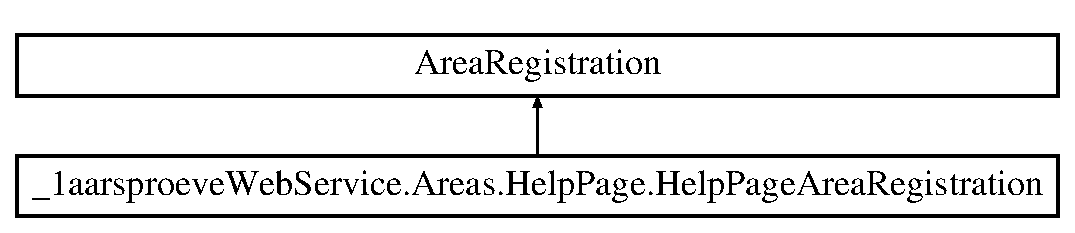
\includegraphics[height=2.000000cm]{class__1aarsproeve_web_service_1_1_areas_1_1_help_page_1_1_help_page_area_registration}
\end{center}
\end{figure}
\subsection*{Public Member Functions}
\begin{DoxyCompactItemize}
\item 
\hypertarget{class__1aarsproeve_web_service_1_1_areas_1_1_help_page_1_1_help_page_area_registration_a2d995fdeaeb65a3da6b712389c462b39}{}override void {\bfseries Register\+Area} (Area\+Registration\+Context context)\label{class__1aarsproeve_web_service_1_1_areas_1_1_help_page_1_1_help_page_area_registration_a2d995fdeaeb65a3da6b712389c462b39}

\end{DoxyCompactItemize}
\subsection*{Properties}
\begin{DoxyCompactItemize}
\item 
\hypertarget{class__1aarsproeve_web_service_1_1_areas_1_1_help_page_1_1_help_page_area_registration_a9402b3b3aba317e0afa36ff4ddf0593f}{}override string {\bfseries Area\+Name}\hspace{0.3cm}{\ttfamily  \mbox{[}get\mbox{]}}\label{class__1aarsproeve_web_service_1_1_areas_1_1_help_page_1_1_help_page_area_registration_a9402b3b3aba317e0afa36ff4ddf0593f}

\end{DoxyCompactItemize}


The documentation for this class was generated from the following file\+:\begin{DoxyCompactItemize}
\item 
C\+:/\+Users/\+Daniel\+Winther/\+Documents/\+Git\+Hub/1-\/aarsproeve/1aarsproeve/1aarsproeve\+Web\+Service/\+Areas/\+Help\+Page/Help\+Page\+Area\+Registration.\+cs\end{DoxyCompactItemize}

\hypertarget{class__1aarsproeve_web_service_1_1_areas_1_1_help_page_1_1_help_page_sample_generator}{}\section{\+\_\+1aarsproeve\+Web\+Service.\+Areas.\+Help\+Page.\+Help\+Page\+Sample\+Generator Class Reference}
\label{class__1aarsproeve_web_service_1_1_areas_1_1_help_page_1_1_help_page_sample_generator}\index{\+\_\+1aarsproeve\+Web\+Service.\+Areas.\+Help\+Page.\+Help\+Page\+Sample\+Generator@{\+\_\+1aarsproeve\+Web\+Service.\+Areas.\+Help\+Page.\+Help\+Page\+Sample\+Generator}}


This class will generate the samples for the help page.  


\subsection*{Public Member Functions}
\begin{DoxyCompactItemize}
\item 
\hyperlink{class__1aarsproeve_web_service_1_1_areas_1_1_help_page_1_1_help_page_sample_generator_aaffd24fef2501eaf464e7096fd4c02a7}{Help\+Page\+Sample\+Generator} ()
\begin{DoxyCompactList}\small\item\em Initializes a new instance of the \hyperlink{class__1aarsproeve_web_service_1_1_areas_1_1_help_page_1_1_help_page_sample_generator}{Help\+Page\+Sample\+Generator} class. \end{DoxyCompactList}\item 
I\+Dictionary$<$ Media\+Type\+Header\+Value, object $>$ \hyperlink{class__1aarsproeve_web_service_1_1_areas_1_1_help_page_1_1_help_page_sample_generator_a9cdb4f0b9852c9000a1519c984ac6f93}{Get\+Sample\+Requests} (Api\+Description api)
\begin{DoxyCompactList}\small\item\em Gets the request body samples for a given Api\+Description. \end{DoxyCompactList}\item 
I\+Dictionary$<$ Media\+Type\+Header\+Value, object $>$ \hyperlink{class__1aarsproeve_web_service_1_1_areas_1_1_help_page_1_1_help_page_sample_generator_a51d80ce95f3d1ed0aaa555a631dc8369}{Get\+Sample\+Responses} (Api\+Description api)
\begin{DoxyCompactList}\small\item\em Gets the response body samples for a given Api\+Description. \end{DoxyCompactList}\item 
virtual I\+Dictionary$<$ Media\+Type\+Header\+Value, object $>$ \hyperlink{class__1aarsproeve_web_service_1_1_areas_1_1_help_page_1_1_help_page_sample_generator_a4838c3b94a8ecabd38c519211ceeaa2b}{Get\+Sample} (Api\+Description api, \hyperlink{namespace__1aarsproeve_web_service_1_1_areas_1_1_help_page_a3b5e2312590d86c11aab0e939d9e102b}{Sample\+Direction} sample\+Direction)
\begin{DoxyCompactList}\small\item\em Gets the request or response body samples. \end{DoxyCompactList}\item 
virtual object \hyperlink{class__1aarsproeve_web_service_1_1_areas_1_1_help_page_1_1_help_page_sample_generator_a4b3866717927c231195a48f1826f99a6}{Get\+Action\+Sample} (string controller\+Name, string action\+Name, I\+Enumerable$<$ string $>$ parameter\+Names, Type type, Media\+Type\+Formatter formatter, Media\+Type\+Header\+Value media\+Type, \hyperlink{namespace__1aarsproeve_web_service_1_1_areas_1_1_help_page_a3b5e2312590d86c11aab0e939d9e102b}{Sample\+Direction} sample\+Direction)
\begin{DoxyCompactList}\small\item\em Search for samples that are provided directly through \hyperlink{class__1aarsproeve_web_service_1_1_areas_1_1_help_page_1_1_help_page_sample_generator_ad0321b323f21617bef877513f585c0a2}{Action\+Samples}. \end{DoxyCompactList}\item 
virtual object \hyperlink{class__1aarsproeve_web_service_1_1_areas_1_1_help_page_1_1_help_page_sample_generator_a5e04c38927cb05f3c416350bd3d8d7d8}{Get\+Sample\+Object} (Type type)
\begin{DoxyCompactList}\small\item\em Gets the sample object that will be serialized by the formatters. First, it will look at the \hyperlink{class__1aarsproeve_web_service_1_1_areas_1_1_help_page_1_1_help_page_sample_generator_aa9621fc1bc0621b656579d3967528dcc}{Sample\+Objects}. If no sample object is found, it will try to create one using Default\+Sample\+Object\+Factory (which wraps an \hyperlink{class__1aarsproeve_web_service_1_1_areas_1_1_help_page_1_1_object_generator}{Object\+Generator}) and other factories in \hyperlink{class__1aarsproeve_web_service_1_1_areas_1_1_help_page_1_1_help_page_sample_generator_a29295b515e45cebc44d8a111e9dd3d01}{Sample\+Object\+Factories}. \end{DoxyCompactList}\item 
virtual Type \hyperlink{class__1aarsproeve_web_service_1_1_areas_1_1_help_page_1_1_help_page_sample_generator_a5040f1ab4783209dd14860fe0b193496}{Resolve\+Http\+Request\+Message\+Type} (Api\+Description api)
\begin{DoxyCompactList}\small\item\em Resolves the actual type of System.\+Net.\+Http.\+Object\+Content$<$\+T$>$ passed to the System.\+Net.\+Http.\+Http\+Request\+Message in an action. \end{DoxyCompactList}\item 
virtual Type \hyperlink{class__1aarsproeve_web_service_1_1_areas_1_1_help_page_1_1_help_page_sample_generator_a4af0718be8a6369e37d905fb131e9448}{Resolve\+Type} (Api\+Description api, string controller\+Name, string action\+Name, I\+Enumerable$<$ string $>$ parameter\+Names, \hyperlink{namespace__1aarsproeve_web_service_1_1_areas_1_1_help_page_a3b5e2312590d86c11aab0e939d9e102b}{Sample\+Direction} sample\+Direction, out Collection$<$ Media\+Type\+Formatter $>$ formatters)
\begin{DoxyCompactList}\small\item\em Resolves the type of the action parameter or return value when Http\+Request\+Message or Http\+Response\+Message is used. \end{DoxyCompactList}\item 
virtual object \hyperlink{class__1aarsproeve_web_service_1_1_areas_1_1_help_page_1_1_help_page_sample_generator_ad78ea8663bf8d54d8a8ce4007ad58dba}{Write\+Sample\+Object\+Using\+Formatter} (Media\+Type\+Formatter formatter, object value, Type type, Media\+Type\+Header\+Value media\+Type)
\begin{DoxyCompactList}\small\item\em Writes the sample object using formatter. \end{DoxyCompactList}\end{DoxyCompactItemize}
\subsection*{Properties}
\begin{DoxyCompactItemize}
\item 
I\+Dictionary$<$ \hyperlink{class__1aarsproeve_web_service_1_1_areas_1_1_help_page_1_1_help_page_sample_key}{Help\+Page\+Sample\+Key}, Type $>$ \hyperlink{class__1aarsproeve_web_service_1_1_areas_1_1_help_page_1_1_help_page_sample_generator_a9f1ac86d102c5386627d7098a52d836f}{Actual\+Http\+Message\+Types}\hspace{0.3cm}{\ttfamily  \mbox{[}get, set\mbox{]}}
\begin{DoxyCompactList}\small\item\em Gets C\+L\+R types that are used as the content of Http\+Request\+Message or Http\+Response\+Message. \end{DoxyCompactList}\item 
I\+Dictionary$<$ \hyperlink{class__1aarsproeve_web_service_1_1_areas_1_1_help_page_1_1_help_page_sample_key}{Help\+Page\+Sample\+Key}, object $>$ \hyperlink{class__1aarsproeve_web_service_1_1_areas_1_1_help_page_1_1_help_page_sample_generator_ad0321b323f21617bef877513f585c0a2}{Action\+Samples}\hspace{0.3cm}{\ttfamily  \mbox{[}get, set\mbox{]}}
\begin{DoxyCompactList}\small\item\em Gets the objects that are used directly as samples for certain actions. \end{DoxyCompactList}\item 
I\+Dictionary$<$ Type, object $>$ \hyperlink{class__1aarsproeve_web_service_1_1_areas_1_1_help_page_1_1_help_page_sample_generator_aa9621fc1bc0621b656579d3967528dcc}{Sample\+Objects}\hspace{0.3cm}{\ttfamily  \mbox{[}get, set\mbox{]}}
\begin{DoxyCompactList}\small\item\em Gets the objects that are serialized as samples by the supported formatters. \end{DoxyCompactList}\item 
I\+List$<$ Func$<$ \hyperlink{class__1aarsproeve_web_service_1_1_areas_1_1_help_page_1_1_help_page_sample_generator}{Help\+Page\+Sample\+Generator}, Type, object $>$ $>$ \hyperlink{class__1aarsproeve_web_service_1_1_areas_1_1_help_page_1_1_help_page_sample_generator_a29295b515e45cebc44d8a111e9dd3d01}{Sample\+Object\+Factories}\hspace{0.3cm}{\ttfamily  \mbox{[}get\mbox{]}}
\begin{DoxyCompactList}\small\item\em Gets factories for the objects that the supported formatters will serialize as samples. Processed in order, stopping when the factory successfully returns a non-\/ object. \end{DoxyCompactList}\end{DoxyCompactItemize}


\subsection{Detailed Description}
This class will generate the samples for the help page. 



\subsection{Constructor \& Destructor Documentation}
\hypertarget{class__1aarsproeve_web_service_1_1_areas_1_1_help_page_1_1_help_page_sample_generator_aaffd24fef2501eaf464e7096fd4c02a7}{}\index{\+\_\+1aarsproeve\+Web\+Service\+::\+Areas\+::\+Help\+Page\+::\+Help\+Page\+Sample\+Generator@{\+\_\+1aarsproeve\+Web\+Service\+::\+Areas\+::\+Help\+Page\+::\+Help\+Page\+Sample\+Generator}!Help\+Page\+Sample\+Generator@{Help\+Page\+Sample\+Generator}}
\index{Help\+Page\+Sample\+Generator@{Help\+Page\+Sample\+Generator}!\+\_\+1aarsproeve\+Web\+Service\+::\+Areas\+::\+Help\+Page\+::\+Help\+Page\+Sample\+Generator@{\+\_\+1aarsproeve\+Web\+Service\+::\+Areas\+::\+Help\+Page\+::\+Help\+Page\+Sample\+Generator}}
\subsubsection[{Help\+Page\+Sample\+Generator}]{\setlength{\rightskip}{0pt plus 5cm}\+\_\+1aarsproeve\+Web\+Service.\+Areas.\+Help\+Page.\+Help\+Page\+Sample\+Generator.\+Help\+Page\+Sample\+Generator (
\begin{DoxyParamCaption}
{}
\end{DoxyParamCaption}
)}\label{class__1aarsproeve_web_service_1_1_areas_1_1_help_page_1_1_help_page_sample_generator_aaffd24fef2501eaf464e7096fd4c02a7}


Initializes a new instance of the \hyperlink{class__1aarsproeve_web_service_1_1_areas_1_1_help_page_1_1_help_page_sample_generator}{Help\+Page\+Sample\+Generator} class. 



\subsection{Member Function Documentation}
\hypertarget{class__1aarsproeve_web_service_1_1_areas_1_1_help_page_1_1_help_page_sample_generator_a4b3866717927c231195a48f1826f99a6}{}\index{\+\_\+1aarsproeve\+Web\+Service\+::\+Areas\+::\+Help\+Page\+::\+Help\+Page\+Sample\+Generator@{\+\_\+1aarsproeve\+Web\+Service\+::\+Areas\+::\+Help\+Page\+::\+Help\+Page\+Sample\+Generator}!Get\+Action\+Sample@{Get\+Action\+Sample}}
\index{Get\+Action\+Sample@{Get\+Action\+Sample}!\+\_\+1aarsproeve\+Web\+Service\+::\+Areas\+::\+Help\+Page\+::\+Help\+Page\+Sample\+Generator@{\+\_\+1aarsproeve\+Web\+Service\+::\+Areas\+::\+Help\+Page\+::\+Help\+Page\+Sample\+Generator}}
\subsubsection[{Get\+Action\+Sample}]{\setlength{\rightskip}{0pt plus 5cm}virtual object \+\_\+1aarsproeve\+Web\+Service.\+Areas.\+Help\+Page.\+Help\+Page\+Sample\+Generator.\+Get\+Action\+Sample (
\begin{DoxyParamCaption}
\item[{string}]{controller\+Name, }
\item[{string}]{action\+Name, }
\item[{I\+Enumerable$<$ string $>$}]{parameter\+Names, }
\item[{Type}]{type, }
\item[{Media\+Type\+Formatter}]{formatter, }
\item[{Media\+Type\+Header\+Value}]{media\+Type, }
\item[{{\bf Sample\+Direction}}]{sample\+Direction}
\end{DoxyParamCaption}
)\hspace{0.3cm}{\ttfamily [virtual]}}\label{class__1aarsproeve_web_service_1_1_areas_1_1_help_page_1_1_help_page_sample_generator_a4b3866717927c231195a48f1826f99a6}


Search for samples that are provided directly through \hyperlink{class__1aarsproeve_web_service_1_1_areas_1_1_help_page_1_1_help_page_sample_generator_ad0321b323f21617bef877513f585c0a2}{Action\+Samples}. 


\begin{DoxyParams}{Parameters}
{\em controller\+Name} & Name of the controller.\\
\hline
{\em action\+Name} & Name of the action.\\
\hline
{\em parameter\+Names} & The parameter names.\\
\hline
{\em type} & The C\+L\+R type.\\
\hline
{\em formatter} & The formatter.\\
\hline
{\em media\+Type} & The media type.\\
\hline
{\em sample\+Direction} & The value indicating whether the sample is for a request or for a response.\\
\hline
\end{DoxyParams}
\begin{DoxyReturn}{Returns}
The sample that matches the parameters.
\end{DoxyReturn}
\hypertarget{class__1aarsproeve_web_service_1_1_areas_1_1_help_page_1_1_help_page_sample_generator_a4838c3b94a8ecabd38c519211ceeaa2b}{}\index{\+\_\+1aarsproeve\+Web\+Service\+::\+Areas\+::\+Help\+Page\+::\+Help\+Page\+Sample\+Generator@{\+\_\+1aarsproeve\+Web\+Service\+::\+Areas\+::\+Help\+Page\+::\+Help\+Page\+Sample\+Generator}!Get\+Sample@{Get\+Sample}}
\index{Get\+Sample@{Get\+Sample}!\+\_\+1aarsproeve\+Web\+Service\+::\+Areas\+::\+Help\+Page\+::\+Help\+Page\+Sample\+Generator@{\+\_\+1aarsproeve\+Web\+Service\+::\+Areas\+::\+Help\+Page\+::\+Help\+Page\+Sample\+Generator}}
\subsubsection[{Get\+Sample}]{\setlength{\rightskip}{0pt plus 5cm}virtual I\+Dictionary$<$Media\+Type\+Header\+Value, object$>$ \+\_\+1aarsproeve\+Web\+Service.\+Areas.\+Help\+Page.\+Help\+Page\+Sample\+Generator.\+Get\+Sample (
\begin{DoxyParamCaption}
\item[{Api\+Description}]{api, }
\item[{{\bf Sample\+Direction}}]{sample\+Direction}
\end{DoxyParamCaption}
)\hspace{0.3cm}{\ttfamily [virtual]}}\label{class__1aarsproeve_web_service_1_1_areas_1_1_help_page_1_1_help_page_sample_generator_a4838c3b94a8ecabd38c519211ceeaa2b}


Gets the request or response body samples. 


\begin{DoxyParams}{Parameters}
{\em api} & The Api\+Description.\\
\hline
{\em sample\+Direction} & The value indicating whether the sample is for a request or for a response.\\
\hline
\end{DoxyParams}
\begin{DoxyReturn}{Returns}
The samples keyed by media type.
\end{DoxyReturn}
\hypertarget{class__1aarsproeve_web_service_1_1_areas_1_1_help_page_1_1_help_page_sample_generator_a5e04c38927cb05f3c416350bd3d8d7d8}{}\index{\+\_\+1aarsproeve\+Web\+Service\+::\+Areas\+::\+Help\+Page\+::\+Help\+Page\+Sample\+Generator@{\+\_\+1aarsproeve\+Web\+Service\+::\+Areas\+::\+Help\+Page\+::\+Help\+Page\+Sample\+Generator}!Get\+Sample\+Object@{Get\+Sample\+Object}}
\index{Get\+Sample\+Object@{Get\+Sample\+Object}!\+\_\+1aarsproeve\+Web\+Service\+::\+Areas\+::\+Help\+Page\+::\+Help\+Page\+Sample\+Generator@{\+\_\+1aarsproeve\+Web\+Service\+::\+Areas\+::\+Help\+Page\+::\+Help\+Page\+Sample\+Generator}}
\subsubsection[{Get\+Sample\+Object}]{\setlength{\rightskip}{0pt plus 5cm}virtual object \+\_\+1aarsproeve\+Web\+Service.\+Areas.\+Help\+Page.\+Help\+Page\+Sample\+Generator.\+Get\+Sample\+Object (
\begin{DoxyParamCaption}
\item[{Type}]{type}
\end{DoxyParamCaption}
)\hspace{0.3cm}{\ttfamily [virtual]}}\label{class__1aarsproeve_web_service_1_1_areas_1_1_help_page_1_1_help_page_sample_generator_a5e04c38927cb05f3c416350bd3d8d7d8}


Gets the sample object that will be serialized by the formatters. First, it will look at the \hyperlink{class__1aarsproeve_web_service_1_1_areas_1_1_help_page_1_1_help_page_sample_generator_aa9621fc1bc0621b656579d3967528dcc}{Sample\+Objects}. If no sample object is found, it will try to create one using Default\+Sample\+Object\+Factory (which wraps an \hyperlink{class__1aarsproeve_web_service_1_1_areas_1_1_help_page_1_1_object_generator}{Object\+Generator}) and other factories in \hyperlink{class__1aarsproeve_web_service_1_1_areas_1_1_help_page_1_1_help_page_sample_generator_a29295b515e45cebc44d8a111e9dd3d01}{Sample\+Object\+Factories}. 


\begin{DoxyParams}{Parameters}
{\em type} & The type.\\
\hline
\end{DoxyParams}
\begin{DoxyReturn}{Returns}
The sample object.
\end{DoxyReturn}
\hypertarget{class__1aarsproeve_web_service_1_1_areas_1_1_help_page_1_1_help_page_sample_generator_a9cdb4f0b9852c9000a1519c984ac6f93}{}\index{\+\_\+1aarsproeve\+Web\+Service\+::\+Areas\+::\+Help\+Page\+::\+Help\+Page\+Sample\+Generator@{\+\_\+1aarsproeve\+Web\+Service\+::\+Areas\+::\+Help\+Page\+::\+Help\+Page\+Sample\+Generator}!Get\+Sample\+Requests@{Get\+Sample\+Requests}}
\index{Get\+Sample\+Requests@{Get\+Sample\+Requests}!\+\_\+1aarsproeve\+Web\+Service\+::\+Areas\+::\+Help\+Page\+::\+Help\+Page\+Sample\+Generator@{\+\_\+1aarsproeve\+Web\+Service\+::\+Areas\+::\+Help\+Page\+::\+Help\+Page\+Sample\+Generator}}
\subsubsection[{Get\+Sample\+Requests}]{\setlength{\rightskip}{0pt plus 5cm}I\+Dictionary$<$Media\+Type\+Header\+Value, object$>$ \+\_\+1aarsproeve\+Web\+Service.\+Areas.\+Help\+Page.\+Help\+Page\+Sample\+Generator.\+Get\+Sample\+Requests (
\begin{DoxyParamCaption}
\item[{Api\+Description}]{api}
\end{DoxyParamCaption}
)}\label{class__1aarsproeve_web_service_1_1_areas_1_1_help_page_1_1_help_page_sample_generator_a9cdb4f0b9852c9000a1519c984ac6f93}


Gets the request body samples for a given Api\+Description. 


\begin{DoxyParams}{Parameters}
{\em api} & The Api\+Description.\\
\hline
\end{DoxyParams}
\begin{DoxyReturn}{Returns}
The samples keyed by media type.
\end{DoxyReturn}
\hypertarget{class__1aarsproeve_web_service_1_1_areas_1_1_help_page_1_1_help_page_sample_generator_a51d80ce95f3d1ed0aaa555a631dc8369}{}\index{\+\_\+1aarsproeve\+Web\+Service\+::\+Areas\+::\+Help\+Page\+::\+Help\+Page\+Sample\+Generator@{\+\_\+1aarsproeve\+Web\+Service\+::\+Areas\+::\+Help\+Page\+::\+Help\+Page\+Sample\+Generator}!Get\+Sample\+Responses@{Get\+Sample\+Responses}}
\index{Get\+Sample\+Responses@{Get\+Sample\+Responses}!\+\_\+1aarsproeve\+Web\+Service\+::\+Areas\+::\+Help\+Page\+::\+Help\+Page\+Sample\+Generator@{\+\_\+1aarsproeve\+Web\+Service\+::\+Areas\+::\+Help\+Page\+::\+Help\+Page\+Sample\+Generator}}
\subsubsection[{Get\+Sample\+Responses}]{\setlength{\rightskip}{0pt plus 5cm}I\+Dictionary$<$Media\+Type\+Header\+Value, object$>$ \+\_\+1aarsproeve\+Web\+Service.\+Areas.\+Help\+Page.\+Help\+Page\+Sample\+Generator.\+Get\+Sample\+Responses (
\begin{DoxyParamCaption}
\item[{Api\+Description}]{api}
\end{DoxyParamCaption}
)}\label{class__1aarsproeve_web_service_1_1_areas_1_1_help_page_1_1_help_page_sample_generator_a51d80ce95f3d1ed0aaa555a631dc8369}


Gets the response body samples for a given Api\+Description. 


\begin{DoxyParams}{Parameters}
{\em api} & The Api\+Description.\\
\hline
\end{DoxyParams}
\begin{DoxyReturn}{Returns}
The samples keyed by media type.
\end{DoxyReturn}
\hypertarget{class__1aarsproeve_web_service_1_1_areas_1_1_help_page_1_1_help_page_sample_generator_a5040f1ab4783209dd14860fe0b193496}{}\index{\+\_\+1aarsproeve\+Web\+Service\+::\+Areas\+::\+Help\+Page\+::\+Help\+Page\+Sample\+Generator@{\+\_\+1aarsproeve\+Web\+Service\+::\+Areas\+::\+Help\+Page\+::\+Help\+Page\+Sample\+Generator}!Resolve\+Http\+Request\+Message\+Type@{Resolve\+Http\+Request\+Message\+Type}}
\index{Resolve\+Http\+Request\+Message\+Type@{Resolve\+Http\+Request\+Message\+Type}!\+\_\+1aarsproeve\+Web\+Service\+::\+Areas\+::\+Help\+Page\+::\+Help\+Page\+Sample\+Generator@{\+\_\+1aarsproeve\+Web\+Service\+::\+Areas\+::\+Help\+Page\+::\+Help\+Page\+Sample\+Generator}}
\subsubsection[{Resolve\+Http\+Request\+Message\+Type}]{\setlength{\rightskip}{0pt plus 5cm}virtual Type \+\_\+1aarsproeve\+Web\+Service.\+Areas.\+Help\+Page.\+Help\+Page\+Sample\+Generator.\+Resolve\+Http\+Request\+Message\+Type (
\begin{DoxyParamCaption}
\item[{Api\+Description}]{api}
\end{DoxyParamCaption}
)\hspace{0.3cm}{\ttfamily [virtual]}}\label{class__1aarsproeve_web_service_1_1_areas_1_1_help_page_1_1_help_page_sample_generator_a5040f1ab4783209dd14860fe0b193496}


Resolves the actual type of System.\+Net.\+Http.\+Object\+Content$<$\+T$>$ passed to the System.\+Net.\+Http.\+Http\+Request\+Message in an action. 


\begin{DoxyParams}{Parameters}
{\em api} & The Api\+Description.\\
\hline
\end{DoxyParams}
\begin{DoxyReturn}{Returns}
The type.
\end{DoxyReturn}
\hypertarget{class__1aarsproeve_web_service_1_1_areas_1_1_help_page_1_1_help_page_sample_generator_a4af0718be8a6369e37d905fb131e9448}{}\index{\+\_\+1aarsproeve\+Web\+Service\+::\+Areas\+::\+Help\+Page\+::\+Help\+Page\+Sample\+Generator@{\+\_\+1aarsproeve\+Web\+Service\+::\+Areas\+::\+Help\+Page\+::\+Help\+Page\+Sample\+Generator}!Resolve\+Type@{Resolve\+Type}}
\index{Resolve\+Type@{Resolve\+Type}!\+\_\+1aarsproeve\+Web\+Service\+::\+Areas\+::\+Help\+Page\+::\+Help\+Page\+Sample\+Generator@{\+\_\+1aarsproeve\+Web\+Service\+::\+Areas\+::\+Help\+Page\+::\+Help\+Page\+Sample\+Generator}}
\subsubsection[{Resolve\+Type}]{\setlength{\rightskip}{0pt plus 5cm}virtual Type \+\_\+1aarsproeve\+Web\+Service.\+Areas.\+Help\+Page.\+Help\+Page\+Sample\+Generator.\+Resolve\+Type (
\begin{DoxyParamCaption}
\item[{Api\+Description}]{api, }
\item[{string}]{controller\+Name, }
\item[{string}]{action\+Name, }
\item[{I\+Enumerable$<$ string $>$}]{parameter\+Names, }
\item[{{\bf Sample\+Direction}}]{sample\+Direction, }
\item[{out Collection$<$ Media\+Type\+Formatter $>$}]{formatters}
\end{DoxyParamCaption}
)\hspace{0.3cm}{\ttfamily [virtual]}}\label{class__1aarsproeve_web_service_1_1_areas_1_1_help_page_1_1_help_page_sample_generator_a4af0718be8a6369e37d905fb131e9448}


Resolves the type of the action parameter or return value when Http\+Request\+Message or Http\+Response\+Message is used. 


\begin{DoxyParams}{Parameters}
{\em api} & The Api\+Description.\\
\hline
{\em controller\+Name} & Name of the controller.\\
\hline
{\em action\+Name} & Name of the action.\\
\hline
{\em parameter\+Names} & The parameter names.\\
\hline
{\em sample\+Direction} & The value indicating whether the sample is for a request or a response.\\
\hline
{\em formatters} & The formatters.\\
\hline
\end{DoxyParams}
\hypertarget{class__1aarsproeve_web_service_1_1_areas_1_1_help_page_1_1_help_page_sample_generator_ad78ea8663bf8d54d8a8ce4007ad58dba}{}\index{\+\_\+1aarsproeve\+Web\+Service\+::\+Areas\+::\+Help\+Page\+::\+Help\+Page\+Sample\+Generator@{\+\_\+1aarsproeve\+Web\+Service\+::\+Areas\+::\+Help\+Page\+::\+Help\+Page\+Sample\+Generator}!Write\+Sample\+Object\+Using\+Formatter@{Write\+Sample\+Object\+Using\+Formatter}}
\index{Write\+Sample\+Object\+Using\+Formatter@{Write\+Sample\+Object\+Using\+Formatter}!\+\_\+1aarsproeve\+Web\+Service\+::\+Areas\+::\+Help\+Page\+::\+Help\+Page\+Sample\+Generator@{\+\_\+1aarsproeve\+Web\+Service\+::\+Areas\+::\+Help\+Page\+::\+Help\+Page\+Sample\+Generator}}
\subsubsection[{Write\+Sample\+Object\+Using\+Formatter}]{\setlength{\rightskip}{0pt plus 5cm}virtual object \+\_\+1aarsproeve\+Web\+Service.\+Areas.\+Help\+Page.\+Help\+Page\+Sample\+Generator.\+Write\+Sample\+Object\+Using\+Formatter (
\begin{DoxyParamCaption}
\item[{Media\+Type\+Formatter}]{formatter, }
\item[{object}]{value, }
\item[{Type}]{type, }
\item[{Media\+Type\+Header\+Value}]{media\+Type}
\end{DoxyParamCaption}
)\hspace{0.3cm}{\ttfamily [virtual]}}\label{class__1aarsproeve_web_service_1_1_areas_1_1_help_page_1_1_help_page_sample_generator_ad78ea8663bf8d54d8a8ce4007ad58dba}


Writes the sample object using formatter. 


\begin{DoxyParams}{Parameters}
{\em formatter} & The formatter.\\
\hline
{\em value} & The value.\\
\hline
{\em type} & The type.\\
\hline
{\em media\+Type} & Type of the media.\\
\hline
\end{DoxyParams}
\begin{DoxyReturn}{Returns}

\end{DoxyReturn}


\subsection{Property Documentation}
\hypertarget{class__1aarsproeve_web_service_1_1_areas_1_1_help_page_1_1_help_page_sample_generator_ad0321b323f21617bef877513f585c0a2}{}\index{\+\_\+1aarsproeve\+Web\+Service\+::\+Areas\+::\+Help\+Page\+::\+Help\+Page\+Sample\+Generator@{\+\_\+1aarsproeve\+Web\+Service\+::\+Areas\+::\+Help\+Page\+::\+Help\+Page\+Sample\+Generator}!Action\+Samples@{Action\+Samples}}
\index{Action\+Samples@{Action\+Samples}!\+\_\+1aarsproeve\+Web\+Service\+::\+Areas\+::\+Help\+Page\+::\+Help\+Page\+Sample\+Generator@{\+\_\+1aarsproeve\+Web\+Service\+::\+Areas\+::\+Help\+Page\+::\+Help\+Page\+Sample\+Generator}}
\subsubsection[{Action\+Samples}]{\setlength{\rightskip}{0pt plus 5cm}I\+Dictionary$<${\bf Help\+Page\+Sample\+Key}, object$>$ \+\_\+1aarsproeve\+Web\+Service.\+Areas.\+Help\+Page.\+Help\+Page\+Sample\+Generator.\+Action\+Samples\hspace{0.3cm}{\ttfamily [get]}, {\ttfamily [set]}}\label{class__1aarsproeve_web_service_1_1_areas_1_1_help_page_1_1_help_page_sample_generator_ad0321b323f21617bef877513f585c0a2}


Gets the objects that are used directly as samples for certain actions. 

\hypertarget{class__1aarsproeve_web_service_1_1_areas_1_1_help_page_1_1_help_page_sample_generator_a9f1ac86d102c5386627d7098a52d836f}{}\index{\+\_\+1aarsproeve\+Web\+Service\+::\+Areas\+::\+Help\+Page\+::\+Help\+Page\+Sample\+Generator@{\+\_\+1aarsproeve\+Web\+Service\+::\+Areas\+::\+Help\+Page\+::\+Help\+Page\+Sample\+Generator}!Actual\+Http\+Message\+Types@{Actual\+Http\+Message\+Types}}
\index{Actual\+Http\+Message\+Types@{Actual\+Http\+Message\+Types}!\+\_\+1aarsproeve\+Web\+Service\+::\+Areas\+::\+Help\+Page\+::\+Help\+Page\+Sample\+Generator@{\+\_\+1aarsproeve\+Web\+Service\+::\+Areas\+::\+Help\+Page\+::\+Help\+Page\+Sample\+Generator}}
\subsubsection[{Actual\+Http\+Message\+Types}]{\setlength{\rightskip}{0pt plus 5cm}I\+Dictionary$<${\bf Help\+Page\+Sample\+Key}, Type$>$ \+\_\+1aarsproeve\+Web\+Service.\+Areas.\+Help\+Page.\+Help\+Page\+Sample\+Generator.\+Actual\+Http\+Message\+Types\hspace{0.3cm}{\ttfamily [get]}, {\ttfamily [set]}}\label{class__1aarsproeve_web_service_1_1_areas_1_1_help_page_1_1_help_page_sample_generator_a9f1ac86d102c5386627d7098a52d836f}


Gets C\+L\+R types that are used as the content of Http\+Request\+Message or Http\+Response\+Message. 

\hypertarget{class__1aarsproeve_web_service_1_1_areas_1_1_help_page_1_1_help_page_sample_generator_a29295b515e45cebc44d8a111e9dd3d01}{}\index{\+\_\+1aarsproeve\+Web\+Service\+::\+Areas\+::\+Help\+Page\+::\+Help\+Page\+Sample\+Generator@{\+\_\+1aarsproeve\+Web\+Service\+::\+Areas\+::\+Help\+Page\+::\+Help\+Page\+Sample\+Generator}!Sample\+Object\+Factories@{Sample\+Object\+Factories}}
\index{Sample\+Object\+Factories@{Sample\+Object\+Factories}!\+\_\+1aarsproeve\+Web\+Service\+::\+Areas\+::\+Help\+Page\+::\+Help\+Page\+Sample\+Generator@{\+\_\+1aarsproeve\+Web\+Service\+::\+Areas\+::\+Help\+Page\+::\+Help\+Page\+Sample\+Generator}}
\subsubsection[{Sample\+Object\+Factories}]{\setlength{\rightskip}{0pt plus 5cm}I\+List$<$Func$<${\bf Help\+Page\+Sample\+Generator}, Type, object$>$ $>$ \+\_\+1aarsproeve\+Web\+Service.\+Areas.\+Help\+Page.\+Help\+Page\+Sample\+Generator.\+Sample\+Object\+Factories\hspace{0.3cm}{\ttfamily [get]}}\label{class__1aarsproeve_web_service_1_1_areas_1_1_help_page_1_1_help_page_sample_generator_a29295b515e45cebc44d8a111e9dd3d01}


Gets factories for the objects that the supported formatters will serialize as samples. Processed in order, stopping when the factory successfully returns a non-\/ object. 

Collection includes just \hyperlink{class__1aarsproeve_web_service_1_1_areas_1_1_help_page_1_1_object_generator_ad47fd6b8894401475144cf522d8767d0}{Object\+Generator.\+Generate\+Object(\+Type)} initially. Use 
\begin{DoxyCode}
\hyperlink{class__1aarsproeve_web_service_1_1_areas_1_1_help_page_1_1_help_page_sample_generator_a29295b515e45cebc44d8a111e9dd3d01}{SampleObjectFactories}.Insert(0, func)
\end{DoxyCode}
 to provide an override and 
\begin{DoxyCode}
\hyperlink{class__1aarsproeve_web_service_1_1_areas_1_1_help_page_1_1_help_page_sample_generator_a29295b515e45cebc44d8a111e9dd3d01}{SampleObjectFactories}.Add(func)
\end{DoxyCode}
 to provide a fallback.\hypertarget{class__1aarsproeve_web_service_1_1_areas_1_1_help_page_1_1_help_page_sample_generator_aa9621fc1bc0621b656579d3967528dcc}{}\index{\+\_\+1aarsproeve\+Web\+Service\+::\+Areas\+::\+Help\+Page\+::\+Help\+Page\+Sample\+Generator@{\+\_\+1aarsproeve\+Web\+Service\+::\+Areas\+::\+Help\+Page\+::\+Help\+Page\+Sample\+Generator}!Sample\+Objects@{Sample\+Objects}}
\index{Sample\+Objects@{Sample\+Objects}!\+\_\+1aarsproeve\+Web\+Service\+::\+Areas\+::\+Help\+Page\+::\+Help\+Page\+Sample\+Generator@{\+\_\+1aarsproeve\+Web\+Service\+::\+Areas\+::\+Help\+Page\+::\+Help\+Page\+Sample\+Generator}}
\subsubsection[{Sample\+Objects}]{\setlength{\rightskip}{0pt plus 5cm}I\+Dictionary$<$Type, object$>$ \+\_\+1aarsproeve\+Web\+Service.\+Areas.\+Help\+Page.\+Help\+Page\+Sample\+Generator.\+Sample\+Objects\hspace{0.3cm}{\ttfamily [get]}, {\ttfamily [set]}}\label{class__1aarsproeve_web_service_1_1_areas_1_1_help_page_1_1_help_page_sample_generator_aa9621fc1bc0621b656579d3967528dcc}


Gets the objects that are serialized as samples by the supported formatters. 



The documentation for this class was generated from the following file\+:\begin{DoxyCompactItemize}
\item 
Documents/\+Git\+Hub/1-\/aarsproeve/1aarsproeve/1aarsproeve\+Web\+Service/\+Areas/\+Help\+Page/\+Sample\+Generation/Help\+Page\+Sample\+Generator.\+cs\end{DoxyCompactItemize}

\hypertarget{class__1aarsproeve_web_service_1_1_areas_1_1_help_page_1_1_help_page_sample_key}{}\section{\+\_\+1aarsproeve\+Web\+Service.\+Areas.\+Help\+Page.\+Help\+Page\+Sample\+Key Class Reference}
\label{class__1aarsproeve_web_service_1_1_areas_1_1_help_page_1_1_help_page_sample_key}\index{\+\_\+1aarsproeve\+Web\+Service.\+Areas.\+Help\+Page.\+Help\+Page\+Sample\+Key@{\+\_\+1aarsproeve\+Web\+Service.\+Areas.\+Help\+Page.\+Help\+Page\+Sample\+Key}}


This is used to identify the place where the sample should be applied.  


\subsection*{Public Member Functions}
\begin{DoxyCompactItemize}
\item 
\hyperlink{class__1aarsproeve_web_service_1_1_areas_1_1_help_page_1_1_help_page_sample_key_ad5ad8423e1346cf212e19637088bc472}{Help\+Page\+Sample\+Key} (Media\+Type\+Header\+Value media\+Type)
\begin{DoxyCompactList}\small\item\em Creates a new \hyperlink{class__1aarsproeve_web_service_1_1_areas_1_1_help_page_1_1_help_page_sample_key}{Help\+Page\+Sample\+Key} based on media type. \end{DoxyCompactList}\item 
\hyperlink{class__1aarsproeve_web_service_1_1_areas_1_1_help_page_1_1_help_page_sample_key_a4170cca4dfffd21164c8ff7a54f20ac5}{Help\+Page\+Sample\+Key} (Media\+Type\+Header\+Value media\+Type, Type type)
\begin{DoxyCompactList}\small\item\em Creates a new \hyperlink{class__1aarsproeve_web_service_1_1_areas_1_1_help_page_1_1_help_page_sample_key}{Help\+Page\+Sample\+Key} based on media type and C\+L\+R type. \end{DoxyCompactList}\item 
\hyperlink{class__1aarsproeve_web_service_1_1_areas_1_1_help_page_1_1_help_page_sample_key_aeaaa386d273efbed71c42137489609b1}{Help\+Page\+Sample\+Key} (\hyperlink{namespace__1aarsproeve_web_service_1_1_areas_1_1_help_page_a3b5e2312590d86c11aab0e939d9e102b}{Sample\+Direction} sample\+Direction, string controller\+Name, string action\+Name, I\+Enumerable$<$ string $>$ parameter\+Names)
\begin{DoxyCompactList}\small\item\em Creates a new \hyperlink{class__1aarsproeve_web_service_1_1_areas_1_1_help_page_1_1_help_page_sample_key}{Help\+Page\+Sample\+Key} based on \hyperlink{class__1aarsproeve_web_service_1_1_areas_1_1_help_page_1_1_help_page_sample_key_a69980321c5a86fc11bbd2d4b3bca84ef}{Sample\+Direction}, controller name, action name and parameter names. \end{DoxyCompactList}\item 
\hyperlink{class__1aarsproeve_web_service_1_1_areas_1_1_help_page_1_1_help_page_sample_key_a37f83ad122302e2e6c2301bf0a7753ba}{Help\+Page\+Sample\+Key} (Media\+Type\+Header\+Value media\+Type, \hyperlink{namespace__1aarsproeve_web_service_1_1_areas_1_1_help_page_a3b5e2312590d86c11aab0e939d9e102b}{Sample\+Direction} sample\+Direction, string controller\+Name, string action\+Name, I\+Enumerable$<$ string $>$ parameter\+Names)
\begin{DoxyCompactList}\small\item\em Creates a new \hyperlink{class__1aarsproeve_web_service_1_1_areas_1_1_help_page_1_1_help_page_sample_key}{Help\+Page\+Sample\+Key} based on media type, \hyperlink{class__1aarsproeve_web_service_1_1_areas_1_1_help_page_1_1_help_page_sample_key_a69980321c5a86fc11bbd2d4b3bca84ef}{Sample\+Direction}, controller name, action name and parameter names. \end{DoxyCompactList}\item 
\hypertarget{class__1aarsproeve_web_service_1_1_areas_1_1_help_page_1_1_help_page_sample_key_aae1ef0cce0c728c5b4b766b6cfb1a19f}{}override bool {\bfseries Equals} (object obj)\label{class__1aarsproeve_web_service_1_1_areas_1_1_help_page_1_1_help_page_sample_key_aae1ef0cce0c728c5b4b766b6cfb1a19f}

\item 
\hypertarget{class__1aarsproeve_web_service_1_1_areas_1_1_help_page_1_1_help_page_sample_key_ab15eabbf1156828a8f95e890cd9b8cca}{}override int {\bfseries Get\+Hash\+Code} ()\label{class__1aarsproeve_web_service_1_1_areas_1_1_help_page_1_1_help_page_sample_key_ab15eabbf1156828a8f95e890cd9b8cca}

\end{DoxyCompactItemize}
\subsection*{Properties}
\begin{DoxyCompactItemize}
\item 
string \hyperlink{class__1aarsproeve_web_service_1_1_areas_1_1_help_page_1_1_help_page_sample_key_a83d3909e7f8daf7ab92060c21afef237}{Controller\+Name}\hspace{0.3cm}{\ttfamily  \mbox{[}get\mbox{]}}
\begin{DoxyCompactList}\small\item\em Gets the name of the controller. \end{DoxyCompactList}\item 
string \hyperlink{class__1aarsproeve_web_service_1_1_areas_1_1_help_page_1_1_help_page_sample_key_abb5930ab215393929bd5fc488c551f32}{Action\+Name}\hspace{0.3cm}{\ttfamily  \mbox{[}get\mbox{]}}
\begin{DoxyCompactList}\small\item\em Gets the name of the action. \end{DoxyCompactList}\item 
Media\+Type\+Header\+Value \hyperlink{class__1aarsproeve_web_service_1_1_areas_1_1_help_page_1_1_help_page_sample_key_a3db7a3c071a64389856208253ce6a8c3}{Media\+Type}\hspace{0.3cm}{\ttfamily  \mbox{[}get\mbox{]}}
\begin{DoxyCompactList}\small\item\em Gets the media type. \end{DoxyCompactList}\item 
Hash\+Set$<$ string $>$ \hyperlink{class__1aarsproeve_web_service_1_1_areas_1_1_help_page_1_1_help_page_sample_key_a2e76cfdbf00172ca1a0dedc0073aeb7b}{Parameter\+Names}\hspace{0.3cm}{\ttfamily  \mbox{[}get\mbox{]}}
\begin{DoxyCompactList}\small\item\em Gets the parameter names. \end{DoxyCompactList}\item 
\hypertarget{class__1aarsproeve_web_service_1_1_areas_1_1_help_page_1_1_help_page_sample_key_a06bee89f6540c17854e99d046dde0163}{}Type {\bfseries Parameter\+Type}\hspace{0.3cm}{\ttfamily  \mbox{[}get\mbox{]}}\label{class__1aarsproeve_web_service_1_1_areas_1_1_help_page_1_1_help_page_sample_key_a06bee89f6540c17854e99d046dde0163}

\item 
\hyperlink{namespace__1aarsproeve_web_service_1_1_areas_1_1_help_page_a3b5e2312590d86c11aab0e939d9e102b}{Sample\+Direction} \hyperlink{class__1aarsproeve_web_service_1_1_areas_1_1_help_page_1_1_help_page_sample_key_a69980321c5a86fc11bbd2d4b3bca84ef}{Sample\+Direction}\hspace{0.3cm}{\ttfamily  \mbox{[}get\mbox{]}}
\begin{DoxyCompactList}\small\item\em Gets the \hyperlink{class__1aarsproeve_web_service_1_1_areas_1_1_help_page_1_1_help_page_sample_key_a69980321c5a86fc11bbd2d4b3bca84ef}{Sample\+Direction}. \end{DoxyCompactList}\end{DoxyCompactItemize}


\subsection{Detailed Description}
This is used to identify the place where the sample should be applied. 



\subsection{Constructor \& Destructor Documentation}
\hypertarget{class__1aarsproeve_web_service_1_1_areas_1_1_help_page_1_1_help_page_sample_key_ad5ad8423e1346cf212e19637088bc472}{}\index{\+\_\+1aarsproeve\+Web\+Service\+::\+Areas\+::\+Help\+Page\+::\+Help\+Page\+Sample\+Key@{\+\_\+1aarsproeve\+Web\+Service\+::\+Areas\+::\+Help\+Page\+::\+Help\+Page\+Sample\+Key}!Help\+Page\+Sample\+Key@{Help\+Page\+Sample\+Key}}
\index{Help\+Page\+Sample\+Key@{Help\+Page\+Sample\+Key}!\+\_\+1aarsproeve\+Web\+Service\+::\+Areas\+::\+Help\+Page\+::\+Help\+Page\+Sample\+Key@{\+\_\+1aarsproeve\+Web\+Service\+::\+Areas\+::\+Help\+Page\+::\+Help\+Page\+Sample\+Key}}
\subsubsection[{Help\+Page\+Sample\+Key}]{\setlength{\rightskip}{0pt plus 5cm}\+\_\+1aarsproeve\+Web\+Service.\+Areas.\+Help\+Page.\+Help\+Page\+Sample\+Key.\+Help\+Page\+Sample\+Key (
\begin{DoxyParamCaption}
\item[{Media\+Type\+Header\+Value}]{media\+Type}
\end{DoxyParamCaption}
)\hspace{0.3cm}{\ttfamily [inline]}}\label{class__1aarsproeve_web_service_1_1_areas_1_1_help_page_1_1_help_page_sample_key_ad5ad8423e1346cf212e19637088bc472}


Creates a new \hyperlink{class__1aarsproeve_web_service_1_1_areas_1_1_help_page_1_1_help_page_sample_key}{Help\+Page\+Sample\+Key} based on media type. 


\begin{DoxyParams}{Parameters}
{\em media\+Type} & The media type.\\
\hline
\end{DoxyParams}
\hypertarget{class__1aarsproeve_web_service_1_1_areas_1_1_help_page_1_1_help_page_sample_key_a4170cca4dfffd21164c8ff7a54f20ac5}{}\index{\+\_\+1aarsproeve\+Web\+Service\+::\+Areas\+::\+Help\+Page\+::\+Help\+Page\+Sample\+Key@{\+\_\+1aarsproeve\+Web\+Service\+::\+Areas\+::\+Help\+Page\+::\+Help\+Page\+Sample\+Key}!Help\+Page\+Sample\+Key@{Help\+Page\+Sample\+Key}}
\index{Help\+Page\+Sample\+Key@{Help\+Page\+Sample\+Key}!\+\_\+1aarsproeve\+Web\+Service\+::\+Areas\+::\+Help\+Page\+::\+Help\+Page\+Sample\+Key@{\+\_\+1aarsproeve\+Web\+Service\+::\+Areas\+::\+Help\+Page\+::\+Help\+Page\+Sample\+Key}}
\subsubsection[{Help\+Page\+Sample\+Key}]{\setlength{\rightskip}{0pt plus 5cm}\+\_\+1aarsproeve\+Web\+Service.\+Areas.\+Help\+Page.\+Help\+Page\+Sample\+Key.\+Help\+Page\+Sample\+Key (
\begin{DoxyParamCaption}
\item[{Media\+Type\+Header\+Value}]{media\+Type, }
\item[{Type}]{type}
\end{DoxyParamCaption}
)\hspace{0.3cm}{\ttfamily [inline]}}\label{class__1aarsproeve_web_service_1_1_areas_1_1_help_page_1_1_help_page_sample_key_a4170cca4dfffd21164c8ff7a54f20ac5}


Creates a new \hyperlink{class__1aarsproeve_web_service_1_1_areas_1_1_help_page_1_1_help_page_sample_key}{Help\+Page\+Sample\+Key} based on media type and C\+L\+R type. 


\begin{DoxyParams}{Parameters}
{\em media\+Type} & The media type.\\
\hline
{\em type} & The C\+L\+R type.\\
\hline
\end{DoxyParams}
\hypertarget{class__1aarsproeve_web_service_1_1_areas_1_1_help_page_1_1_help_page_sample_key_aeaaa386d273efbed71c42137489609b1}{}\index{\+\_\+1aarsproeve\+Web\+Service\+::\+Areas\+::\+Help\+Page\+::\+Help\+Page\+Sample\+Key@{\+\_\+1aarsproeve\+Web\+Service\+::\+Areas\+::\+Help\+Page\+::\+Help\+Page\+Sample\+Key}!Help\+Page\+Sample\+Key@{Help\+Page\+Sample\+Key}}
\index{Help\+Page\+Sample\+Key@{Help\+Page\+Sample\+Key}!\+\_\+1aarsproeve\+Web\+Service\+::\+Areas\+::\+Help\+Page\+::\+Help\+Page\+Sample\+Key@{\+\_\+1aarsproeve\+Web\+Service\+::\+Areas\+::\+Help\+Page\+::\+Help\+Page\+Sample\+Key}}
\subsubsection[{Help\+Page\+Sample\+Key}]{\setlength{\rightskip}{0pt plus 5cm}\+\_\+1aarsproeve\+Web\+Service.\+Areas.\+Help\+Page.\+Help\+Page\+Sample\+Key.\+Help\+Page\+Sample\+Key (
\begin{DoxyParamCaption}
\item[{{\bf Sample\+Direction}}]{sample\+Direction, }
\item[{string}]{controller\+Name, }
\item[{string}]{action\+Name, }
\item[{I\+Enumerable$<$ string $>$}]{parameter\+Names}
\end{DoxyParamCaption}
)\hspace{0.3cm}{\ttfamily [inline]}}\label{class__1aarsproeve_web_service_1_1_areas_1_1_help_page_1_1_help_page_sample_key_aeaaa386d273efbed71c42137489609b1}


Creates a new \hyperlink{class__1aarsproeve_web_service_1_1_areas_1_1_help_page_1_1_help_page_sample_key}{Help\+Page\+Sample\+Key} based on \hyperlink{class__1aarsproeve_web_service_1_1_areas_1_1_help_page_1_1_help_page_sample_key_a69980321c5a86fc11bbd2d4b3bca84ef}{Sample\+Direction}, controller name, action name and parameter names. 


\begin{DoxyParams}{Parameters}
{\em sample\+Direction} & The \hyperlink{class__1aarsproeve_web_service_1_1_areas_1_1_help_page_1_1_help_page_sample_key_a69980321c5a86fc11bbd2d4b3bca84ef}{Sample\+Direction}.\\
\hline
{\em controller\+Name} & Name of the controller.\\
\hline
{\em action\+Name} & Name of the action.\\
\hline
{\em parameter\+Names} & The parameter names.\\
\hline
\end{DoxyParams}
\hypertarget{class__1aarsproeve_web_service_1_1_areas_1_1_help_page_1_1_help_page_sample_key_a37f83ad122302e2e6c2301bf0a7753ba}{}\index{\+\_\+1aarsproeve\+Web\+Service\+::\+Areas\+::\+Help\+Page\+::\+Help\+Page\+Sample\+Key@{\+\_\+1aarsproeve\+Web\+Service\+::\+Areas\+::\+Help\+Page\+::\+Help\+Page\+Sample\+Key}!Help\+Page\+Sample\+Key@{Help\+Page\+Sample\+Key}}
\index{Help\+Page\+Sample\+Key@{Help\+Page\+Sample\+Key}!\+\_\+1aarsproeve\+Web\+Service\+::\+Areas\+::\+Help\+Page\+::\+Help\+Page\+Sample\+Key@{\+\_\+1aarsproeve\+Web\+Service\+::\+Areas\+::\+Help\+Page\+::\+Help\+Page\+Sample\+Key}}
\subsubsection[{Help\+Page\+Sample\+Key}]{\setlength{\rightskip}{0pt plus 5cm}\+\_\+1aarsproeve\+Web\+Service.\+Areas.\+Help\+Page.\+Help\+Page\+Sample\+Key.\+Help\+Page\+Sample\+Key (
\begin{DoxyParamCaption}
\item[{Media\+Type\+Header\+Value}]{media\+Type, }
\item[{{\bf Sample\+Direction}}]{sample\+Direction, }
\item[{string}]{controller\+Name, }
\item[{string}]{action\+Name, }
\item[{I\+Enumerable$<$ string $>$}]{parameter\+Names}
\end{DoxyParamCaption}
)\hspace{0.3cm}{\ttfamily [inline]}}\label{class__1aarsproeve_web_service_1_1_areas_1_1_help_page_1_1_help_page_sample_key_a37f83ad122302e2e6c2301bf0a7753ba}


Creates a new \hyperlink{class__1aarsproeve_web_service_1_1_areas_1_1_help_page_1_1_help_page_sample_key}{Help\+Page\+Sample\+Key} based on media type, \hyperlink{class__1aarsproeve_web_service_1_1_areas_1_1_help_page_1_1_help_page_sample_key_a69980321c5a86fc11bbd2d4b3bca84ef}{Sample\+Direction}, controller name, action name and parameter names. 


\begin{DoxyParams}{Parameters}
{\em media\+Type} & The media type.\\
\hline
{\em sample\+Direction} & The \hyperlink{class__1aarsproeve_web_service_1_1_areas_1_1_help_page_1_1_help_page_sample_key_a69980321c5a86fc11bbd2d4b3bca84ef}{Sample\+Direction}.\\
\hline
{\em controller\+Name} & Name of the controller.\\
\hline
{\em action\+Name} & Name of the action.\\
\hline
{\em parameter\+Names} & The parameter names.\\
\hline
\end{DoxyParams}


\subsection{Property Documentation}
\hypertarget{class__1aarsproeve_web_service_1_1_areas_1_1_help_page_1_1_help_page_sample_key_abb5930ab215393929bd5fc488c551f32}{}\index{\+\_\+1aarsproeve\+Web\+Service\+::\+Areas\+::\+Help\+Page\+::\+Help\+Page\+Sample\+Key@{\+\_\+1aarsproeve\+Web\+Service\+::\+Areas\+::\+Help\+Page\+::\+Help\+Page\+Sample\+Key}!Action\+Name@{Action\+Name}}
\index{Action\+Name@{Action\+Name}!\+\_\+1aarsproeve\+Web\+Service\+::\+Areas\+::\+Help\+Page\+::\+Help\+Page\+Sample\+Key@{\+\_\+1aarsproeve\+Web\+Service\+::\+Areas\+::\+Help\+Page\+::\+Help\+Page\+Sample\+Key}}
\subsubsection[{Action\+Name}]{\setlength{\rightskip}{0pt plus 5cm}string \+\_\+1aarsproeve\+Web\+Service.\+Areas.\+Help\+Page.\+Help\+Page\+Sample\+Key.\+Action\+Name\hspace{0.3cm}{\ttfamily [get]}}\label{class__1aarsproeve_web_service_1_1_areas_1_1_help_page_1_1_help_page_sample_key_abb5930ab215393929bd5fc488c551f32}


Gets the name of the action. 

The name of the action. \hypertarget{class__1aarsproeve_web_service_1_1_areas_1_1_help_page_1_1_help_page_sample_key_a83d3909e7f8daf7ab92060c21afef237}{}\index{\+\_\+1aarsproeve\+Web\+Service\+::\+Areas\+::\+Help\+Page\+::\+Help\+Page\+Sample\+Key@{\+\_\+1aarsproeve\+Web\+Service\+::\+Areas\+::\+Help\+Page\+::\+Help\+Page\+Sample\+Key}!Controller\+Name@{Controller\+Name}}
\index{Controller\+Name@{Controller\+Name}!\+\_\+1aarsproeve\+Web\+Service\+::\+Areas\+::\+Help\+Page\+::\+Help\+Page\+Sample\+Key@{\+\_\+1aarsproeve\+Web\+Service\+::\+Areas\+::\+Help\+Page\+::\+Help\+Page\+Sample\+Key}}
\subsubsection[{Controller\+Name}]{\setlength{\rightskip}{0pt plus 5cm}string \+\_\+1aarsproeve\+Web\+Service.\+Areas.\+Help\+Page.\+Help\+Page\+Sample\+Key.\+Controller\+Name\hspace{0.3cm}{\ttfamily [get]}}\label{class__1aarsproeve_web_service_1_1_areas_1_1_help_page_1_1_help_page_sample_key_a83d3909e7f8daf7ab92060c21afef237}


Gets the name of the controller. 

The name of the controller. \hypertarget{class__1aarsproeve_web_service_1_1_areas_1_1_help_page_1_1_help_page_sample_key_a3db7a3c071a64389856208253ce6a8c3}{}\index{\+\_\+1aarsproeve\+Web\+Service\+::\+Areas\+::\+Help\+Page\+::\+Help\+Page\+Sample\+Key@{\+\_\+1aarsproeve\+Web\+Service\+::\+Areas\+::\+Help\+Page\+::\+Help\+Page\+Sample\+Key}!Media\+Type@{Media\+Type}}
\index{Media\+Type@{Media\+Type}!\+\_\+1aarsproeve\+Web\+Service\+::\+Areas\+::\+Help\+Page\+::\+Help\+Page\+Sample\+Key@{\+\_\+1aarsproeve\+Web\+Service\+::\+Areas\+::\+Help\+Page\+::\+Help\+Page\+Sample\+Key}}
\subsubsection[{Media\+Type}]{\setlength{\rightskip}{0pt plus 5cm}Media\+Type\+Header\+Value \+\_\+1aarsproeve\+Web\+Service.\+Areas.\+Help\+Page.\+Help\+Page\+Sample\+Key.\+Media\+Type\hspace{0.3cm}{\ttfamily [get]}}\label{class__1aarsproeve_web_service_1_1_areas_1_1_help_page_1_1_help_page_sample_key_a3db7a3c071a64389856208253ce6a8c3}


Gets the media type. 

The media type. \hypertarget{class__1aarsproeve_web_service_1_1_areas_1_1_help_page_1_1_help_page_sample_key_a2e76cfdbf00172ca1a0dedc0073aeb7b}{}\index{\+\_\+1aarsproeve\+Web\+Service\+::\+Areas\+::\+Help\+Page\+::\+Help\+Page\+Sample\+Key@{\+\_\+1aarsproeve\+Web\+Service\+::\+Areas\+::\+Help\+Page\+::\+Help\+Page\+Sample\+Key}!Parameter\+Names@{Parameter\+Names}}
\index{Parameter\+Names@{Parameter\+Names}!\+\_\+1aarsproeve\+Web\+Service\+::\+Areas\+::\+Help\+Page\+::\+Help\+Page\+Sample\+Key@{\+\_\+1aarsproeve\+Web\+Service\+::\+Areas\+::\+Help\+Page\+::\+Help\+Page\+Sample\+Key}}
\subsubsection[{Parameter\+Names}]{\setlength{\rightskip}{0pt plus 5cm}Hash\+Set$<$string$>$ \+\_\+1aarsproeve\+Web\+Service.\+Areas.\+Help\+Page.\+Help\+Page\+Sample\+Key.\+Parameter\+Names\hspace{0.3cm}{\ttfamily [get]}}\label{class__1aarsproeve_web_service_1_1_areas_1_1_help_page_1_1_help_page_sample_key_a2e76cfdbf00172ca1a0dedc0073aeb7b}


Gets the parameter names. 

\hypertarget{class__1aarsproeve_web_service_1_1_areas_1_1_help_page_1_1_help_page_sample_key_a69980321c5a86fc11bbd2d4b3bca84ef}{}\index{\+\_\+1aarsproeve\+Web\+Service\+::\+Areas\+::\+Help\+Page\+::\+Help\+Page\+Sample\+Key@{\+\_\+1aarsproeve\+Web\+Service\+::\+Areas\+::\+Help\+Page\+::\+Help\+Page\+Sample\+Key}!Sample\+Direction@{Sample\+Direction}}
\index{Sample\+Direction@{Sample\+Direction}!\+\_\+1aarsproeve\+Web\+Service\+::\+Areas\+::\+Help\+Page\+::\+Help\+Page\+Sample\+Key@{\+\_\+1aarsproeve\+Web\+Service\+::\+Areas\+::\+Help\+Page\+::\+Help\+Page\+Sample\+Key}}
\subsubsection[{Sample\+Direction}]{\setlength{\rightskip}{0pt plus 5cm}{\bf Sample\+Direction} \+\_\+1aarsproeve\+Web\+Service.\+Areas.\+Help\+Page.\+Help\+Page\+Sample\+Key.\+Sample\+Direction\hspace{0.3cm}{\ttfamily [get]}}\label{class__1aarsproeve_web_service_1_1_areas_1_1_help_page_1_1_help_page_sample_key_a69980321c5a86fc11bbd2d4b3bca84ef}


Gets the \hyperlink{class__1aarsproeve_web_service_1_1_areas_1_1_help_page_1_1_help_page_sample_key_a69980321c5a86fc11bbd2d4b3bca84ef}{Sample\+Direction}. 



The documentation for this class was generated from the following file\+:\begin{DoxyCompactItemize}
\item 
Documents/\+Git\+Hub/1-\/aarsproeve/1aarsproeve/1aarsproeve\+Web\+Service/\+Areas/\+Help\+Page/\+Sample\+Generation/Help\+Page\+Sample\+Key.\+cs\end{DoxyCompactItemize}

\hypertarget{class__1aarsproeve_web_service_1_1_controllers_1_1_home_controller}{}\section{\+\_\+1aarsproeve\+Web\+Service.\+Controllers.\+Home\+Controller Class Reference}
\label{class__1aarsproeve_web_service_1_1_controllers_1_1_home_controller}\index{\+\_\+1aarsproeve\+Web\+Service.\+Controllers.\+Home\+Controller@{\+\_\+1aarsproeve\+Web\+Service.\+Controllers.\+Home\+Controller}}
Inheritance diagram for \+\_\+1aarsproeve\+Web\+Service.\+Controllers.\+Home\+Controller\+:\begin{figure}[H]
\begin{center}
\leavevmode
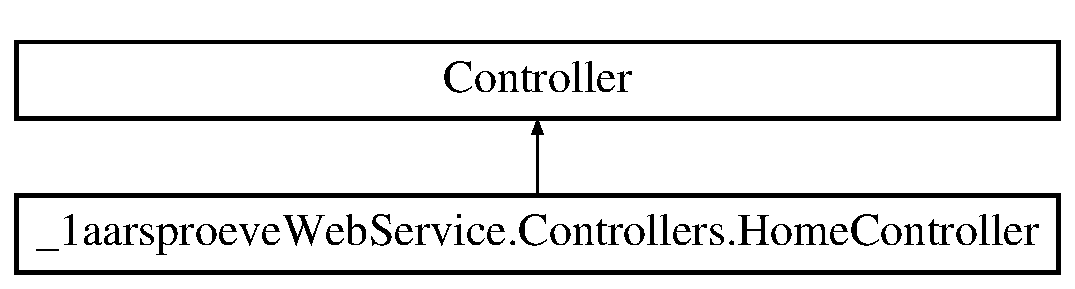
\includegraphics[height=2.000000cm]{class__1aarsproeve_web_service_1_1_controllers_1_1_home_controller}
\end{center}
\end{figure}
\subsection*{Public Member Functions}
\begin{DoxyCompactItemize}
\item 
\hypertarget{class__1aarsproeve_web_service_1_1_controllers_1_1_home_controller_afeaf8faefb53b2651fbdcbd4c743496c}{}Action\+Result {\bfseries Index} ()\label{class__1aarsproeve_web_service_1_1_controllers_1_1_home_controller_afeaf8faefb53b2651fbdcbd4c743496c}

\end{DoxyCompactItemize}


The documentation for this class was generated from the following file\+:\begin{DoxyCompactItemize}
\item 
C\+:/\+Users/\+Daniel\+Winther/\+Documents/\+Git\+Hub/1-\/aarsproeve/1aarsproeve/1aarsproeve\+Web\+Service/\+Controllers/Home\+Controller.\+cs\end{DoxyCompactItemize}

\hypertarget{class__1aarsproeve_1_1_view_1_1_hovedmenu}{}\section{\+\_\+1aarsproeve.\+View.\+Hovedmenu Class Reference}
\label{class__1aarsproeve_1_1_view_1_1_hovedmenu}\index{\+\_\+1aarsproeve.\+View.\+Hovedmenu@{\+\_\+1aarsproeve.\+View.\+Hovedmenu}}


A basic page that provides characteristics common to most applications.  


Inheritance diagram for \+\_\+1aarsproeve.\+View.\+Hovedmenu\+:\begin{figure}[H]
\begin{center}
\leavevmode
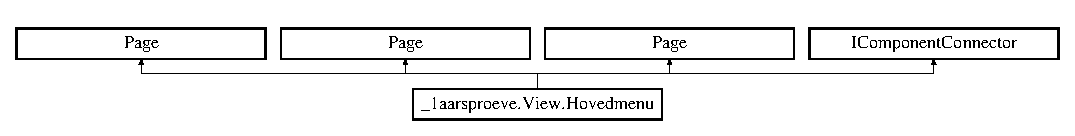
\includegraphics[height=1.386139cm]{class__1aarsproeve_1_1_view_1_1_hovedmenu}
\end{center}
\end{figure}
\subsection*{Public Member Functions}
\begin{DoxyCompactItemize}
\item 
\hypertarget{class__1aarsproeve_1_1_view_1_1_hovedmenu_aeed9485754ac62ab25597d6404e433bc}{}void {\bfseries Connect} (int connection\+Id, object target)\label{class__1aarsproeve_1_1_view_1_1_hovedmenu_aeed9485754ac62ab25597d6404e433bc}

\item 
\hypertarget{class__1aarsproeve_1_1_view_1_1_hovedmenu_add366b00659bb8e885d9d771115edd45}{}void {\bfseries Initialize\+Component} ()\label{class__1aarsproeve_1_1_view_1_1_hovedmenu_add366b00659bb8e885d9d771115edd45}

\end{DoxyCompactItemize}
\subsection*{Protected Member Functions}
\begin{DoxyCompactItemize}
\item 
override void \hyperlink{class__1aarsproeve_1_1_view_1_1_hovedmenu_a4dcfaf095ce527ff701f5422c81e96a8}{On\+Navigated\+To} (Navigation\+Event\+Args e)
\item 
\hypertarget{class__1aarsproeve_1_1_view_1_1_hovedmenu_a74e7e27fd04a768bf9314dc870cb1ef6}{}override void {\bfseries On\+Navigated\+From} (Navigation\+Event\+Args e)\label{class__1aarsproeve_1_1_view_1_1_hovedmenu_a74e7e27fd04a768bf9314dc870cb1ef6}

\end{DoxyCompactItemize}
\subsection*{Properties}
\begin{DoxyCompactItemize}
\item 
\hyperlink{class__1aarsproeve_1_1_common_1_1_observable_dictionary}{Observable\+Dictionary} \hyperlink{class__1aarsproeve_1_1_view_1_1_hovedmenu_a190a68175b53527c294361f545270777}{Default\+View\+Model}\hspace{0.3cm}{\ttfamily  \mbox{[}get\mbox{]}}
\begin{DoxyCompactList}\small\item\em This can be changed to a strongly typed view model. \end{DoxyCompactList}\item 
\hyperlink{class__1aarsproeve_1_1_common_1_1_navigation_helper}{Navigation\+Helper} \hyperlink{class__1aarsproeve_1_1_view_1_1_hovedmenu_ac513dbcbc4b71272c5590cb997863925}{Navigation\+Helper}\hspace{0.3cm}{\ttfamily  \mbox{[}get\mbox{]}}
\begin{DoxyCompactList}\small\item\em Navigation\+Helper is used on each page to aid in navigation and process lifetime management \end{DoxyCompactList}\end{DoxyCompactItemize}


\subsection{Detailed Description}
A basic page that provides characteristics common to most applications. 



\subsection{Member Function Documentation}
\hypertarget{class__1aarsproeve_1_1_view_1_1_hovedmenu_a4dcfaf095ce527ff701f5422c81e96a8}{}\index{\+\_\+1aarsproeve\+::\+View\+::\+Hovedmenu@{\+\_\+1aarsproeve\+::\+View\+::\+Hovedmenu}!On\+Navigated\+To@{On\+Navigated\+To}}
\index{On\+Navigated\+To@{On\+Navigated\+To}!\+\_\+1aarsproeve\+::\+View\+::\+Hovedmenu@{\+\_\+1aarsproeve\+::\+View\+::\+Hovedmenu}}
\subsubsection[{On\+Navigated\+To}]{\setlength{\rightskip}{0pt plus 5cm}override void \+\_\+1aarsproeve.\+View.\+Hovedmenu.\+On\+Navigated\+To (
\begin{DoxyParamCaption}
\item[{Navigation\+Event\+Args}]{e}
\end{DoxyParamCaption}
)\hspace{0.3cm}{\ttfamily [inline]}, {\ttfamily [protected]}}\label{class__1aarsproeve_1_1_view_1_1_hovedmenu_a4dcfaf095ce527ff701f5422c81e96a8}
The methods provided in this section are simply used to allow Navigation\+Helper to respond to the page\textquotesingle{}s navigation methods.

Page specific logic should be placed in event handlers for the Grid\+C\+S.\+Common.\+Navigation\+Helper.\+Load\+State and Grid\+C\+S.\+Common.\+Navigation\+Helper.\+Save\+State. The navigation parameter is available in the Load\+State method in addition to page state preserved during an earlier session. 

\subsection{Property Documentation}
\hypertarget{class__1aarsproeve_1_1_view_1_1_hovedmenu_a190a68175b53527c294361f545270777}{}\index{\+\_\+1aarsproeve\+::\+View\+::\+Hovedmenu@{\+\_\+1aarsproeve\+::\+View\+::\+Hovedmenu}!Default\+View\+Model@{Default\+View\+Model}}
\index{Default\+View\+Model@{Default\+View\+Model}!\+\_\+1aarsproeve\+::\+View\+::\+Hovedmenu@{\+\_\+1aarsproeve\+::\+View\+::\+Hovedmenu}}
\subsubsection[{Default\+View\+Model}]{\setlength{\rightskip}{0pt plus 5cm}{\bf Observable\+Dictionary} \+\_\+1aarsproeve.\+View.\+Hovedmenu.\+Default\+View\+Model\hspace{0.3cm}{\ttfamily [get]}}\label{class__1aarsproeve_1_1_view_1_1_hovedmenu_a190a68175b53527c294361f545270777}


This can be changed to a strongly typed view model. 

\hypertarget{class__1aarsproeve_1_1_view_1_1_hovedmenu_ac513dbcbc4b71272c5590cb997863925}{}\index{\+\_\+1aarsproeve\+::\+View\+::\+Hovedmenu@{\+\_\+1aarsproeve\+::\+View\+::\+Hovedmenu}!Navigation\+Helper@{Navigation\+Helper}}
\index{Navigation\+Helper@{Navigation\+Helper}!\+\_\+1aarsproeve\+::\+View\+::\+Hovedmenu@{\+\_\+1aarsproeve\+::\+View\+::\+Hovedmenu}}
\subsubsection[{Navigation\+Helper}]{\setlength{\rightskip}{0pt plus 5cm}{\bf Navigation\+Helper} \+\_\+1aarsproeve.\+View.\+Hovedmenu.\+Navigation\+Helper\hspace{0.3cm}{\ttfamily [get]}}\label{class__1aarsproeve_1_1_view_1_1_hovedmenu_ac513dbcbc4b71272c5590cb997863925}


Navigation\+Helper is used on each page to aid in navigation and process lifetime management 



The documentation for this class was generated from the following files\+:\begin{DoxyCompactItemize}
\item 
Documents/\+Git\+Hub/1-\/aarsproeve/1aarsproeve/1aarsproeve/obj/\+Debug/\+View/Hovedmenu.\+g.\+cs\item 
Documents/\+Git\+Hub/1-\/aarsproeve/1aarsproeve/1aarsproeve/obj/\+Debug/\+View/Hovedmenu.\+g.\+i.\+cs\item 
Documents/\+Git\+Hub/1-\/aarsproeve/1aarsproeve/1aarsproeve/\+View/Hovedmenu.\+xaml.\+cs\end{DoxyCompactItemize}

\hypertarget{class__1aarsproeve_1_1_view_model_1_1_hoved_view_model}{}\section{\+\_\+1aarsproeve.\+View\+Model.\+Hoved\+View\+Model Class Reference}
\label{class__1aarsproeve_1_1_view_model_1_1_hoved_view_model}\index{\+\_\+1aarsproeve.\+View\+Model.\+Hoved\+View\+Model@{\+\_\+1aarsproeve.\+View\+Model.\+Hoved\+View\+Model}}


Data\+Context klasse til Views\+: Hovedmenu, Skriv\+Besked  


\subsection*{Public Member Functions}
\begin{DoxyCompactItemize}
\item 
\hyperlink{class__1aarsproeve_1_1_view_model_1_1_hoved_view_model_ad1f93a3cec1e8f3b2272a4e92adb2815}{Hoved\+View\+Model} ()
\begin{DoxyCompactList}\small\item\em Constructor for \hyperlink{class__1aarsproeve_1_1_view_model_1_1_hoved_view_model}{Hoved\+View\+Model} \end{DoxyCompactList}\item 
void \hyperlink{class__1aarsproeve_1_1_view_model_1_1_hoved_view_model_a68003d432c3635ed670f816338720c9a}{Initialiser\+Anmodninger} ()
\begin{DoxyCompactList}\small\item\em Initialiserer anmodninger\+Anmodninger\+Model \end{DoxyCompactList}\end{DoxyCompactItemize}
\subsection*{Properties}
\begin{DoxyCompactItemize}
\item 
static \hyperlink{class__1aarsproeve_1_1_model_1_1_anmodning_model}{Anmodning\+Model} \hyperlink{class__1aarsproeve_1_1_view_model_1_1_hoved_view_model_ab4a4d861215f4d6f8d5ca53382d88d8d}{Selected\+Anmodning}\hspace{0.3cm}{\ttfamily  \mbox{[}get, set\mbox{]}}
\begin{DoxyCompactList}\small\item\em Selected\+Vagter static property \end{DoxyCompactList}\item 
\hypertarget{class__1aarsproeve_1_1_view_model_1_1_hoved_view_model_a36a44e96dd4fe24af2130c2fac90f1b0}{}Observable\+Collection$<$ \hyperlink{class__1aarsproeve_1_1_model_1_1_anmodning_model}{Anmodning\+Model} $>$ {\bfseries Anmodning\+Collection}\hspace{0.3cm}{\ttfamily  \mbox{[}get, set\mbox{]}}\label{class__1aarsproeve_1_1_view_model_1_1_hoved_view_model_a36a44e96dd4fe24af2130c2fac90f1b0}

\item 
Observable\+Collection$<$ \hyperlink{class__1aarsproeve_1_1_model_1_1_besked_model}{Besked\+Model} $>$ \hyperlink{class__1aarsproeve_1_1_view_model_1_1_hoved_view_model_a098905f543f118e9bf1f6fe5143a4741}{Besked\+Collection}\hspace{0.3cm}{\ttfamily  \mbox{[}get, set\mbox{]}}
\begin{DoxyCompactList}\small\item\em Singleton vagtcollection \end{DoxyCompactList}\item 
Application\+Data\+Container \hyperlink{class__1aarsproeve_1_1_view_model_1_1_hoved_view_model_afbb2eb2f33bdb6defe9979b80c6e79ff}{Setting}\hspace{0.3cm}{\ttfamily  \mbox{[}get, set\mbox{]}}
\begin{DoxyCompactList}\small\item\em Gør det muligt at gemme værdier i local storage \end{DoxyCompactList}\item 
string \hyperlink{class__1aarsproeve_1_1_view_model_1_1_hoved_view_model_a48f0c876a1e3cd598fe3c4c7c65a760d}{Brugernavn}\hspace{0.3cm}{\ttfamily  \mbox{[}get, set\mbox{]}}
\begin{DoxyCompactList}\small\item\em Brugernavn property \end{DoxyCompactList}\item 
\hyperlink{class__1aarsproeve_1_1_handler_1_1_hoved_handler}{Hoved\+Handler} \hyperlink{class__1aarsproeve_1_1_view_model_1_1_hoved_view_model_aaeba819c1330608f58f968d670367c47}{Hoved\+Handler}\hspace{0.3cm}{\ttfamily  \mbox{[}get, set\mbox{]}}
\begin{DoxyCompactList}\small\item\em Hovedhandler property \end{DoxyCompactList}\item 
Visibility \hyperlink{class__1aarsproeve_1_1_view_model_1_1_hoved_view_model_ab292f28c3e469ad73d6d6e648f3096f0}{Skjul\+Knap}\hspace{0.3cm}{\ttfamily  \mbox{[}get, set\mbox{]}}
\begin{DoxyCompactList}\small\item\em Skjul\+Knap property \end{DoxyCompactList}\item 
string \hyperlink{class__1aarsproeve_1_1_view_model_1_1_hoved_view_model_a358015de6da111dbb14cc14d7a0a421a}{Ingen\+Anmodninger}\hspace{0.3cm}{\ttfamily  \mbox{[}get, set\mbox{]}}
\begin{DoxyCompactList}\small\item\em Ingen\+Anmodninger property \end{DoxyCompactList}\item 
I\+Command \hyperlink{class__1aarsproeve_1_1_view_model_1_1_hoved_view_model_a7f36282e82a32f8ea520ec676e53bcae}{Selected\+Anmodninger\+Command}\hspace{0.3cm}{\ttfamily  \mbox{[}get, set\mbox{]}}
\begin{DoxyCompactList}\small\item\em Selected\+Anmodninger\+Command property \end{DoxyCompactList}\item 
\hypertarget{class__1aarsproeve_1_1_view_model_1_1_hoved_view_model_a0dcfb8149e0a57bfa65b3466857ee907}{}I\+Command {\bfseries Accepter\+Anmodning\+Command}\hspace{0.3cm}{\ttfamily  \mbox{[}get, set\mbox{]}}\label{class__1aarsproeve_1_1_view_model_1_1_hoved_view_model_a0dcfb8149e0a57bfa65b3466857ee907}

\item 
\hypertarget{class__1aarsproeve_1_1_view_model_1_1_hoved_view_model_aa3f28de12b1a14db3659b56a5797d724}{}I\+Command {\bfseries Annuller\+Anmodning\+Command}\hspace{0.3cm}{\ttfamily  \mbox{[}get, set\mbox{]}}\label{class__1aarsproeve_1_1_view_model_1_1_hoved_view_model_aa3f28de12b1a14db3659b56a5797d724}

\item 
I\+Command \hyperlink{class__1aarsproeve_1_1_view_model_1_1_hoved_view_model_a72688ca49a29be5fc3fa18d16449387e}{Skriv\+Besked\+Command}\hspace{0.3cm}{\ttfamily  \mbox{[}get, set\mbox{]}}
\begin{DoxyCompactList}\small\item\em Skriv\+Besked command \end{DoxyCompactList}\item 
I\+Command \hyperlink{class__1aarsproeve_1_1_view_model_1_1_hoved_view_model_ae541527e8e9063cc3337b229b93c7e48}{Log\+Ud\+Command}\hspace{0.3cm}{\ttfamily  \mbox{[}get, set\mbox{]}}
\begin{DoxyCompactList}\small\item\em Logger brugeren ud \end{DoxyCompactList}\end{DoxyCompactItemize}


\subsection{Detailed Description}
Data\+Context klasse til Views\+: Hovedmenu, Skriv\+Besked 



\subsection{Constructor \& Destructor Documentation}
\hypertarget{class__1aarsproeve_1_1_view_model_1_1_hoved_view_model_ad1f93a3cec1e8f3b2272a4e92adb2815}{}\index{\+\_\+1aarsproeve\+::\+View\+Model\+::\+Hoved\+View\+Model@{\+\_\+1aarsproeve\+::\+View\+Model\+::\+Hoved\+View\+Model}!Hoved\+View\+Model@{Hoved\+View\+Model}}
\index{Hoved\+View\+Model@{Hoved\+View\+Model}!\+\_\+1aarsproeve\+::\+View\+Model\+::\+Hoved\+View\+Model@{\+\_\+1aarsproeve\+::\+View\+Model\+::\+Hoved\+View\+Model}}
\subsubsection[{Hoved\+View\+Model}]{\setlength{\rightskip}{0pt plus 5cm}\+\_\+1aarsproeve.\+View\+Model.\+Hoved\+View\+Model.\+Hoved\+View\+Model (
\begin{DoxyParamCaption}
{}
\end{DoxyParamCaption}
)}\label{class__1aarsproeve_1_1_view_model_1_1_hoved_view_model_ad1f93a3cec1e8f3b2272a4e92adb2815}


Constructor for \hyperlink{class__1aarsproeve_1_1_view_model_1_1_hoved_view_model}{Hoved\+View\+Model} 



\subsection{Member Function Documentation}
\hypertarget{class__1aarsproeve_1_1_view_model_1_1_hoved_view_model_a68003d432c3635ed670f816338720c9a}{}\index{\+\_\+1aarsproeve\+::\+View\+Model\+::\+Hoved\+View\+Model@{\+\_\+1aarsproeve\+::\+View\+Model\+::\+Hoved\+View\+Model}!Initialiser\+Anmodninger@{Initialiser\+Anmodninger}}
\index{Initialiser\+Anmodninger@{Initialiser\+Anmodninger}!\+\_\+1aarsproeve\+::\+View\+Model\+::\+Hoved\+View\+Model@{\+\_\+1aarsproeve\+::\+View\+Model\+::\+Hoved\+View\+Model}}
\subsubsection[{Initialiser\+Anmodninger}]{\setlength{\rightskip}{0pt plus 5cm}void \+\_\+1aarsproeve.\+View\+Model.\+Hoved\+View\+Model.\+Initialiser\+Anmodninger (
\begin{DoxyParamCaption}
{}
\end{DoxyParamCaption}
)}\label{class__1aarsproeve_1_1_view_model_1_1_hoved_view_model_a68003d432c3635ed670f816338720c9a}


Initialiserer anmodninger\+Anmodninger\+Model 



\subsection{Property Documentation}
\hypertarget{class__1aarsproeve_1_1_view_model_1_1_hoved_view_model_a098905f543f118e9bf1f6fe5143a4741}{}\index{\+\_\+1aarsproeve\+::\+View\+Model\+::\+Hoved\+View\+Model@{\+\_\+1aarsproeve\+::\+View\+Model\+::\+Hoved\+View\+Model}!Besked\+Collection@{Besked\+Collection}}
\index{Besked\+Collection@{Besked\+Collection}!\+\_\+1aarsproeve\+::\+View\+Model\+::\+Hoved\+View\+Model@{\+\_\+1aarsproeve\+::\+View\+Model\+::\+Hoved\+View\+Model}}
\subsubsection[{Besked\+Collection}]{\setlength{\rightskip}{0pt plus 5cm}Observable\+Collection$<${\bf Besked\+Model}$>$ \+\_\+1aarsproeve.\+View\+Model.\+Hoved\+View\+Model.\+Besked\+Collection\hspace{0.3cm}{\ttfamily [get]}, {\ttfamily [set]}}\label{class__1aarsproeve_1_1_view_model_1_1_hoved_view_model_a098905f543f118e9bf1f6fe5143a4741}


Singleton vagtcollection 

\hypertarget{class__1aarsproeve_1_1_view_model_1_1_hoved_view_model_a48f0c876a1e3cd598fe3c4c7c65a760d}{}\index{\+\_\+1aarsproeve\+::\+View\+Model\+::\+Hoved\+View\+Model@{\+\_\+1aarsproeve\+::\+View\+Model\+::\+Hoved\+View\+Model}!Brugernavn@{Brugernavn}}
\index{Brugernavn@{Brugernavn}!\+\_\+1aarsproeve\+::\+View\+Model\+::\+Hoved\+View\+Model@{\+\_\+1aarsproeve\+::\+View\+Model\+::\+Hoved\+View\+Model}}
\subsubsection[{Brugernavn}]{\setlength{\rightskip}{0pt plus 5cm}string \+\_\+1aarsproeve.\+View\+Model.\+Hoved\+View\+Model.\+Brugernavn\hspace{0.3cm}{\ttfamily [get]}, {\ttfamily [set]}}\label{class__1aarsproeve_1_1_view_model_1_1_hoved_view_model_a48f0c876a1e3cd598fe3c4c7c65a760d}


Brugernavn property 

\hypertarget{class__1aarsproeve_1_1_view_model_1_1_hoved_view_model_aaeba819c1330608f58f968d670367c47}{}\index{\+\_\+1aarsproeve\+::\+View\+Model\+::\+Hoved\+View\+Model@{\+\_\+1aarsproeve\+::\+View\+Model\+::\+Hoved\+View\+Model}!Hoved\+Handler@{Hoved\+Handler}}
\index{Hoved\+Handler@{Hoved\+Handler}!\+\_\+1aarsproeve\+::\+View\+Model\+::\+Hoved\+View\+Model@{\+\_\+1aarsproeve\+::\+View\+Model\+::\+Hoved\+View\+Model}}
\subsubsection[{Hoved\+Handler}]{\setlength{\rightskip}{0pt plus 5cm}{\bf Hoved\+Handler} \+\_\+1aarsproeve.\+View\+Model.\+Hoved\+View\+Model.\+Hoved\+Handler\hspace{0.3cm}{\ttfamily [get]}, {\ttfamily [set]}}\label{class__1aarsproeve_1_1_view_model_1_1_hoved_view_model_aaeba819c1330608f58f968d670367c47}


Hovedhandler property 

\hypertarget{class__1aarsproeve_1_1_view_model_1_1_hoved_view_model_a358015de6da111dbb14cc14d7a0a421a}{}\index{\+\_\+1aarsproeve\+::\+View\+Model\+::\+Hoved\+View\+Model@{\+\_\+1aarsproeve\+::\+View\+Model\+::\+Hoved\+View\+Model}!Ingen\+Anmodninger@{Ingen\+Anmodninger}}
\index{Ingen\+Anmodninger@{Ingen\+Anmodninger}!\+\_\+1aarsproeve\+::\+View\+Model\+::\+Hoved\+View\+Model@{\+\_\+1aarsproeve\+::\+View\+Model\+::\+Hoved\+View\+Model}}
\subsubsection[{Ingen\+Anmodninger}]{\setlength{\rightskip}{0pt plus 5cm}string \+\_\+1aarsproeve.\+View\+Model.\+Hoved\+View\+Model.\+Ingen\+Anmodninger\hspace{0.3cm}{\ttfamily [get]}, {\ttfamily [set]}}\label{class__1aarsproeve_1_1_view_model_1_1_hoved_view_model_a358015de6da111dbb14cc14d7a0a421a}


Ingen\+Anmodninger property 

\hypertarget{class__1aarsproeve_1_1_view_model_1_1_hoved_view_model_ae541527e8e9063cc3337b229b93c7e48}{}\index{\+\_\+1aarsproeve\+::\+View\+Model\+::\+Hoved\+View\+Model@{\+\_\+1aarsproeve\+::\+View\+Model\+::\+Hoved\+View\+Model}!Log\+Ud\+Command@{Log\+Ud\+Command}}
\index{Log\+Ud\+Command@{Log\+Ud\+Command}!\+\_\+1aarsproeve\+::\+View\+Model\+::\+Hoved\+View\+Model@{\+\_\+1aarsproeve\+::\+View\+Model\+::\+Hoved\+View\+Model}}
\subsubsection[{Log\+Ud\+Command}]{\setlength{\rightskip}{0pt plus 5cm}I\+Command \+\_\+1aarsproeve.\+View\+Model.\+Hoved\+View\+Model.\+Log\+Ud\+Command\hspace{0.3cm}{\ttfamily [get]}, {\ttfamily [set]}}\label{class__1aarsproeve_1_1_view_model_1_1_hoved_view_model_ae541527e8e9063cc3337b229b93c7e48}


Logger brugeren ud 

\hypertarget{class__1aarsproeve_1_1_view_model_1_1_hoved_view_model_ab4a4d861215f4d6f8d5ca53382d88d8d}{}\index{\+\_\+1aarsproeve\+::\+View\+Model\+::\+Hoved\+View\+Model@{\+\_\+1aarsproeve\+::\+View\+Model\+::\+Hoved\+View\+Model}!Selected\+Anmodning@{Selected\+Anmodning}}
\index{Selected\+Anmodning@{Selected\+Anmodning}!\+\_\+1aarsproeve\+::\+View\+Model\+::\+Hoved\+View\+Model@{\+\_\+1aarsproeve\+::\+View\+Model\+::\+Hoved\+View\+Model}}
\subsubsection[{Selected\+Anmodning}]{\setlength{\rightskip}{0pt plus 5cm}{\bf Anmodning\+Model} \+\_\+1aarsproeve.\+View\+Model.\+Hoved\+View\+Model.\+Selected\+Anmodning\hspace{0.3cm}{\ttfamily [static]}, {\ttfamily [get]}, {\ttfamily [set]}}\label{class__1aarsproeve_1_1_view_model_1_1_hoved_view_model_ab4a4d861215f4d6f8d5ca53382d88d8d}


Selected\+Vagter static property 

\hypertarget{class__1aarsproeve_1_1_view_model_1_1_hoved_view_model_a7f36282e82a32f8ea520ec676e53bcae}{}\index{\+\_\+1aarsproeve\+::\+View\+Model\+::\+Hoved\+View\+Model@{\+\_\+1aarsproeve\+::\+View\+Model\+::\+Hoved\+View\+Model}!Selected\+Anmodninger\+Command@{Selected\+Anmodninger\+Command}}
\index{Selected\+Anmodninger\+Command@{Selected\+Anmodninger\+Command}!\+\_\+1aarsproeve\+::\+View\+Model\+::\+Hoved\+View\+Model@{\+\_\+1aarsproeve\+::\+View\+Model\+::\+Hoved\+View\+Model}}
\subsubsection[{Selected\+Anmodninger\+Command}]{\setlength{\rightskip}{0pt plus 5cm}I\+Command \+\_\+1aarsproeve.\+View\+Model.\+Hoved\+View\+Model.\+Selected\+Anmodninger\+Command\hspace{0.3cm}{\ttfamily [get]}, {\ttfamily [set]}}\label{class__1aarsproeve_1_1_view_model_1_1_hoved_view_model_a7f36282e82a32f8ea520ec676e53bcae}


Selected\+Anmodninger\+Command property 

\hypertarget{class__1aarsproeve_1_1_view_model_1_1_hoved_view_model_afbb2eb2f33bdb6defe9979b80c6e79ff}{}\index{\+\_\+1aarsproeve\+::\+View\+Model\+::\+Hoved\+View\+Model@{\+\_\+1aarsproeve\+::\+View\+Model\+::\+Hoved\+View\+Model}!Setting@{Setting}}
\index{Setting@{Setting}!\+\_\+1aarsproeve\+::\+View\+Model\+::\+Hoved\+View\+Model@{\+\_\+1aarsproeve\+::\+View\+Model\+::\+Hoved\+View\+Model}}
\subsubsection[{Setting}]{\setlength{\rightskip}{0pt plus 5cm}Application\+Data\+Container \+\_\+1aarsproeve.\+View\+Model.\+Hoved\+View\+Model.\+Setting\hspace{0.3cm}{\ttfamily [get]}, {\ttfamily [set]}}\label{class__1aarsproeve_1_1_view_model_1_1_hoved_view_model_afbb2eb2f33bdb6defe9979b80c6e79ff}


Gør det muligt at gemme værdier i local storage 

\hypertarget{class__1aarsproeve_1_1_view_model_1_1_hoved_view_model_ab292f28c3e469ad73d6d6e648f3096f0}{}\index{\+\_\+1aarsproeve\+::\+View\+Model\+::\+Hoved\+View\+Model@{\+\_\+1aarsproeve\+::\+View\+Model\+::\+Hoved\+View\+Model}!Skjul\+Knap@{Skjul\+Knap}}
\index{Skjul\+Knap@{Skjul\+Knap}!\+\_\+1aarsproeve\+::\+View\+Model\+::\+Hoved\+View\+Model@{\+\_\+1aarsproeve\+::\+View\+Model\+::\+Hoved\+View\+Model}}
\subsubsection[{Skjul\+Knap}]{\setlength{\rightskip}{0pt plus 5cm}Visibility \+\_\+1aarsproeve.\+View\+Model.\+Hoved\+View\+Model.\+Skjul\+Knap\hspace{0.3cm}{\ttfamily [get]}, {\ttfamily [set]}}\label{class__1aarsproeve_1_1_view_model_1_1_hoved_view_model_ab292f28c3e469ad73d6d6e648f3096f0}


Skjul\+Knap property 

\hypertarget{class__1aarsproeve_1_1_view_model_1_1_hoved_view_model_a72688ca49a29be5fc3fa18d16449387e}{}\index{\+\_\+1aarsproeve\+::\+View\+Model\+::\+Hoved\+View\+Model@{\+\_\+1aarsproeve\+::\+View\+Model\+::\+Hoved\+View\+Model}!Skriv\+Besked\+Command@{Skriv\+Besked\+Command}}
\index{Skriv\+Besked\+Command@{Skriv\+Besked\+Command}!\+\_\+1aarsproeve\+::\+View\+Model\+::\+Hoved\+View\+Model@{\+\_\+1aarsproeve\+::\+View\+Model\+::\+Hoved\+View\+Model}}
\subsubsection[{Skriv\+Besked\+Command}]{\setlength{\rightskip}{0pt plus 5cm}I\+Command \+\_\+1aarsproeve.\+View\+Model.\+Hoved\+View\+Model.\+Skriv\+Besked\+Command\hspace{0.3cm}{\ttfamily [get]}, {\ttfamily [set]}}\label{class__1aarsproeve_1_1_view_model_1_1_hoved_view_model_a72688ca49a29be5fc3fa18d16449387e}


Skriv\+Besked command 



The documentation for this class was generated from the following file\+:\begin{DoxyCompactItemize}
\item 
Documents/\+Git\+Hub/1-\/aarsproeve/1aarsproeve/1aarsproeve/\+View\+Model/Hoved\+View\+Model.\+cs\end{DoxyCompactItemize}

\hypertarget{class__1aarsproeve_web_service_1_1_areas_1_1_help_page_1_1_image_sample}{}\section{\+\_\+1aarsproeve\+Web\+Service.\+Areas.\+Help\+Page.\+Image\+Sample Class Reference}
\label{class__1aarsproeve_web_service_1_1_areas_1_1_help_page_1_1_image_sample}\index{\+\_\+1aarsproeve\+Web\+Service.\+Areas.\+Help\+Page.\+Image\+Sample@{\+\_\+1aarsproeve\+Web\+Service.\+Areas.\+Help\+Page.\+Image\+Sample}}


This represents an image sample on the help page. There\textquotesingle{}s a display template named \hyperlink{class__1aarsproeve_web_service_1_1_areas_1_1_help_page_1_1_image_sample}{Image\+Sample} associated with this class.  


\subsection*{Public Member Functions}
\begin{DoxyCompactItemize}
\item 
\hyperlink{class__1aarsproeve_web_service_1_1_areas_1_1_help_page_1_1_image_sample_a1e2df780051c1af035bdaba293c69c16}{Image\+Sample} (string src)
\begin{DoxyCompactList}\small\item\em Initializes a new instance of the \hyperlink{class__1aarsproeve_web_service_1_1_areas_1_1_help_page_1_1_image_sample}{Image\+Sample} class. \end{DoxyCompactList}\item 
\hypertarget{class__1aarsproeve_web_service_1_1_areas_1_1_help_page_1_1_image_sample_a88789358633abe9acb1e29001576baf7}{}override bool {\bfseries Equals} (object obj)\label{class__1aarsproeve_web_service_1_1_areas_1_1_help_page_1_1_image_sample_a88789358633abe9acb1e29001576baf7}

\item 
\hypertarget{class__1aarsproeve_web_service_1_1_areas_1_1_help_page_1_1_image_sample_ad489923ace1fb65638e7ac2961e46af0}{}override int {\bfseries Get\+Hash\+Code} ()\label{class__1aarsproeve_web_service_1_1_areas_1_1_help_page_1_1_image_sample_ad489923ace1fb65638e7ac2961e46af0}

\item 
\hypertarget{class__1aarsproeve_web_service_1_1_areas_1_1_help_page_1_1_image_sample_a8f0eef1536d1864d9bcc71ccf3e5c86f}{}override string {\bfseries To\+String} ()\label{class__1aarsproeve_web_service_1_1_areas_1_1_help_page_1_1_image_sample_a8f0eef1536d1864d9bcc71ccf3e5c86f}

\end{DoxyCompactItemize}
\subsection*{Properties}
\begin{DoxyCompactItemize}
\item 
\hypertarget{class__1aarsproeve_web_service_1_1_areas_1_1_help_page_1_1_image_sample_adf71f5dae61073430fa38a51937ca45b}{}string {\bfseries Src}\hspace{0.3cm}{\ttfamily  \mbox{[}get\mbox{]}}\label{class__1aarsproeve_web_service_1_1_areas_1_1_help_page_1_1_image_sample_adf71f5dae61073430fa38a51937ca45b}

\end{DoxyCompactItemize}


\subsection{Detailed Description}
This represents an image sample on the help page. There\textquotesingle{}s a display template named \hyperlink{class__1aarsproeve_web_service_1_1_areas_1_1_help_page_1_1_image_sample}{Image\+Sample} associated with this class. 



\subsection{Constructor \& Destructor Documentation}
\hypertarget{class__1aarsproeve_web_service_1_1_areas_1_1_help_page_1_1_image_sample_a1e2df780051c1af035bdaba293c69c16}{}\index{\+\_\+1aarsproeve\+Web\+Service\+::\+Areas\+::\+Help\+Page\+::\+Image\+Sample@{\+\_\+1aarsproeve\+Web\+Service\+::\+Areas\+::\+Help\+Page\+::\+Image\+Sample}!Image\+Sample@{Image\+Sample}}
\index{Image\+Sample@{Image\+Sample}!\+\_\+1aarsproeve\+Web\+Service\+::\+Areas\+::\+Help\+Page\+::\+Image\+Sample@{\+\_\+1aarsproeve\+Web\+Service\+::\+Areas\+::\+Help\+Page\+::\+Image\+Sample}}
\subsubsection[{Image\+Sample}]{\setlength{\rightskip}{0pt plus 5cm}\+\_\+1aarsproeve\+Web\+Service.\+Areas.\+Help\+Page.\+Image\+Sample.\+Image\+Sample (
\begin{DoxyParamCaption}
\item[{string}]{src}
\end{DoxyParamCaption}
)\hspace{0.3cm}{\ttfamily [inline]}}\label{class__1aarsproeve_web_service_1_1_areas_1_1_help_page_1_1_image_sample_a1e2df780051c1af035bdaba293c69c16}


Initializes a new instance of the \hyperlink{class__1aarsproeve_web_service_1_1_areas_1_1_help_page_1_1_image_sample}{Image\+Sample} class. 


\begin{DoxyParams}{Parameters}
{\em src} & The U\+R\+L of an image.\\
\hline
\end{DoxyParams}


The documentation for this class was generated from the following file\+:\begin{DoxyCompactItemize}
\item 
C\+:/\+Users/\+Daniel\+Winther/\+Documents/\+Git\+Hub/1-\/aarsproeve/1aarsproeve/1aarsproeve\+Web\+Service/\+Areas/\+Help\+Page/\+Sample\+Generation/Image\+Sample.\+cs\end{DoxyCompactItemize}

\hypertarget{interface__1aarsproeve_web_service_1_1_areas_1_1_help_page_1_1_model_descriptions_1_1_i_model_documentation_provider}{}\section{\+\_\+1aarsproeve\+Web\+Service.\+Areas.\+Help\+Page.\+Model\+Descriptions.\+I\+Model\+Documentation\+Provider Interface Reference}
\label{interface__1aarsproeve_web_service_1_1_areas_1_1_help_page_1_1_model_descriptions_1_1_i_model_documentation_provider}\index{\+\_\+1aarsproeve\+Web\+Service.\+Areas.\+Help\+Page.\+Model\+Descriptions.\+I\+Model\+Documentation\+Provider@{\+\_\+1aarsproeve\+Web\+Service.\+Areas.\+Help\+Page.\+Model\+Descriptions.\+I\+Model\+Documentation\+Provider}}
Inheritance diagram for \+\_\+1aarsproeve\+Web\+Service.\+Areas.\+Help\+Page.\+Model\+Descriptions.\+I\+Model\+Documentation\+Provider\+:\begin{figure}[H]
\begin{center}
\leavevmode
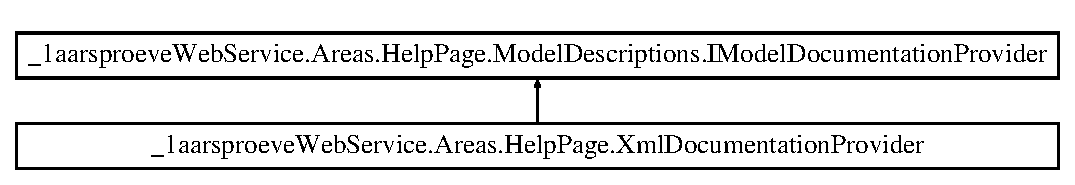
\includegraphics[height=2.000000cm]{interface__1aarsproeve_web_service_1_1_areas_1_1_help_page_1_1_model_descriptions_1_1_i_model_documentation_provider}
\end{center}
\end{figure}
\subsection*{Public Member Functions}
\begin{DoxyCompactItemize}
\item 
\hypertarget{interface__1aarsproeve_web_service_1_1_areas_1_1_help_page_1_1_model_descriptions_1_1_i_model_documentation_provider_a2b728d776da74168bd405ae202c11129}{}string {\bfseries Get\+Documentation} (Member\+Info member)\label{interface__1aarsproeve_web_service_1_1_areas_1_1_help_page_1_1_model_descriptions_1_1_i_model_documentation_provider_a2b728d776da74168bd405ae202c11129}

\item 
\hypertarget{interface__1aarsproeve_web_service_1_1_areas_1_1_help_page_1_1_model_descriptions_1_1_i_model_documentation_provider_a0c90877deffb5cdbfb8260caa8ab7411}{}string {\bfseries Get\+Documentation} (Type type)\label{interface__1aarsproeve_web_service_1_1_areas_1_1_help_page_1_1_model_descriptions_1_1_i_model_documentation_provider_a0c90877deffb5cdbfb8260caa8ab7411}

\end{DoxyCompactItemize}


The documentation for this interface was generated from the following file\+:\begin{DoxyCompactItemize}
\item 
Documents/\+Git\+Hub/1-\/aarsproeve/1aarsproeve/1aarsproeve\+Web\+Service/\+Areas/\+Help\+Page/\+Model\+Descriptions/I\+Model\+Documentation\+Provider.\+cs\end{DoxyCompactItemize}

\hypertarget{class__1aarsproeve_web_service_1_1_areas_1_1_help_page_1_1_invalid_sample}{}\section{\+\_\+1aarsproeve\+Web\+Service.\+Areas.\+Help\+Page.\+Invalid\+Sample Class Reference}
\label{class__1aarsproeve_web_service_1_1_areas_1_1_help_page_1_1_invalid_sample}\index{\+\_\+1aarsproeve\+Web\+Service.\+Areas.\+Help\+Page.\+Invalid\+Sample@{\+\_\+1aarsproeve\+Web\+Service.\+Areas.\+Help\+Page.\+Invalid\+Sample}}


This represents an invalid sample on the help page. There\textquotesingle{}s a display template named \hyperlink{class__1aarsproeve_web_service_1_1_areas_1_1_help_page_1_1_invalid_sample}{Invalid\+Sample} associated with this class.  


\subsection*{Public Member Functions}
\begin{DoxyCompactItemize}
\item 
\hypertarget{class__1aarsproeve_web_service_1_1_areas_1_1_help_page_1_1_invalid_sample_a1765a67a11a267d2a02438471821a853}{}{\bfseries Invalid\+Sample} (string error\+Message)\label{class__1aarsproeve_web_service_1_1_areas_1_1_help_page_1_1_invalid_sample_a1765a67a11a267d2a02438471821a853}

\item 
\hypertarget{class__1aarsproeve_web_service_1_1_areas_1_1_help_page_1_1_invalid_sample_a6cad532356f4b19d8b3175e5a0b15ce2}{}override bool {\bfseries Equals} (object obj)\label{class__1aarsproeve_web_service_1_1_areas_1_1_help_page_1_1_invalid_sample_a6cad532356f4b19d8b3175e5a0b15ce2}

\item 
\hypertarget{class__1aarsproeve_web_service_1_1_areas_1_1_help_page_1_1_invalid_sample_ab5b125556be4287c86458a81926863bd}{}override int {\bfseries Get\+Hash\+Code} ()\label{class__1aarsproeve_web_service_1_1_areas_1_1_help_page_1_1_invalid_sample_ab5b125556be4287c86458a81926863bd}

\item 
\hypertarget{class__1aarsproeve_web_service_1_1_areas_1_1_help_page_1_1_invalid_sample_a5ee58359dbb090cde32a683584f5fdd2}{}override string {\bfseries To\+String} ()\label{class__1aarsproeve_web_service_1_1_areas_1_1_help_page_1_1_invalid_sample_a5ee58359dbb090cde32a683584f5fdd2}

\end{DoxyCompactItemize}
\subsection*{Properties}
\begin{DoxyCompactItemize}
\item 
\hypertarget{class__1aarsproeve_web_service_1_1_areas_1_1_help_page_1_1_invalid_sample_aa93907902bb52616392de80e5d603f0b}{}string {\bfseries Error\+Message}\hspace{0.3cm}{\ttfamily  \mbox{[}get\mbox{]}}\label{class__1aarsproeve_web_service_1_1_areas_1_1_help_page_1_1_invalid_sample_aa93907902bb52616392de80e5d603f0b}

\end{DoxyCompactItemize}


\subsection{Detailed Description}
This represents an invalid sample on the help page. There\textquotesingle{}s a display template named \hyperlink{class__1aarsproeve_web_service_1_1_areas_1_1_help_page_1_1_invalid_sample}{Invalid\+Sample} associated with this class. 



The documentation for this class was generated from the following file\+:\begin{DoxyCompactItemize}
\item 
C\+:/\+Users/\+Daniel\+Winther/\+Documents/\+Git\+Hub/1-\/aarsproeve/1aarsproeve/1aarsproeve\+Web\+Service/\+Areas/\+Help\+Page/\+Sample\+Generation/Invalid\+Sample.\+cs\end{DoxyCompactItemize}

\hypertarget{class__1aarsproeve_web_service_1_1_areas_1_1_help_page_1_1_model_descriptions_1_1_key_value_pair_model_description}{}\section{\+\_\+1aarsproeve\+Web\+Service.\+Areas.\+Help\+Page.\+Model\+Descriptions.\+Key\+Value\+Pair\+Model\+Description Class Reference}
\label{class__1aarsproeve_web_service_1_1_areas_1_1_help_page_1_1_model_descriptions_1_1_key_value_pair_model_description}\index{\+\_\+1aarsproeve\+Web\+Service.\+Areas.\+Help\+Page.\+Model\+Descriptions.\+Key\+Value\+Pair\+Model\+Description@{\+\_\+1aarsproeve\+Web\+Service.\+Areas.\+Help\+Page.\+Model\+Descriptions.\+Key\+Value\+Pair\+Model\+Description}}
Inheritance diagram for \+\_\+1aarsproeve\+Web\+Service.\+Areas.\+Help\+Page.\+Model\+Descriptions.\+Key\+Value\+Pair\+Model\+Description\+:\begin{figure}[H]
\begin{center}
\leavevmode
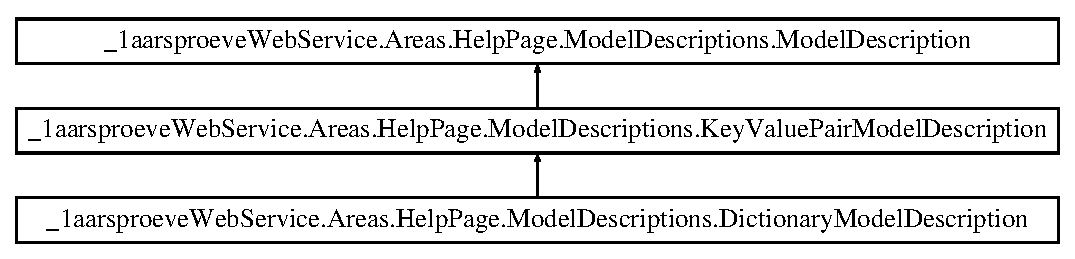
\includegraphics[height=3.000000cm]{class__1aarsproeve_web_service_1_1_areas_1_1_help_page_1_1_model_descriptions_1_1_key_value_pair_model_description}
\end{center}
\end{figure}
\subsection*{Properties}
\begin{DoxyCompactItemize}
\item 
\hypertarget{class__1aarsproeve_web_service_1_1_areas_1_1_help_page_1_1_model_descriptions_1_1_key_value_pair_model_description_a23fe709521a85919c682b4ab9a011bef}{}\hyperlink{class__1aarsproeve_web_service_1_1_areas_1_1_help_page_1_1_model_descriptions_1_1_model_description}{Model\+Description} {\bfseries Key\+Model\+Description}\hspace{0.3cm}{\ttfamily  \mbox{[}get, set\mbox{]}}\label{class__1aarsproeve_web_service_1_1_areas_1_1_help_page_1_1_model_descriptions_1_1_key_value_pair_model_description_a23fe709521a85919c682b4ab9a011bef}

\item 
\hypertarget{class__1aarsproeve_web_service_1_1_areas_1_1_help_page_1_1_model_descriptions_1_1_key_value_pair_model_description_a93b416f7ebe2d8515d8b483d7518ea3b}{}\hyperlink{class__1aarsproeve_web_service_1_1_areas_1_1_help_page_1_1_model_descriptions_1_1_model_description}{Model\+Description} {\bfseries Value\+Model\+Description}\hspace{0.3cm}{\ttfamily  \mbox{[}get, set\mbox{]}}\label{class__1aarsproeve_web_service_1_1_areas_1_1_help_page_1_1_model_descriptions_1_1_key_value_pair_model_description_a93b416f7ebe2d8515d8b483d7518ea3b}

\end{DoxyCompactItemize}


The documentation for this class was generated from the following file\+:\begin{DoxyCompactItemize}
\item 
C\+:/\+Users/\+Daniel\+Winther/\+Documents/\+Git\+Hub/1-\/aarsproeve/1aarsproeve/1aarsproeve\+Web\+Service/\+Areas/\+Help\+Page/\+Model\+Descriptions/Key\+Value\+Pair\+Model\+Description.\+cs\end{DoxyCompactItemize}

\hypertarget{class__1aarsproeve_1_1_common_1_1_load_state_event_args}{}\section{\+\_\+1aarsproeve.\+Common.\+Load\+State\+Event\+Args Class Reference}
\label{class__1aarsproeve_1_1_common_1_1_load_state_event_args}\index{\+\_\+1aarsproeve.\+Common.\+Load\+State\+Event\+Args@{\+\_\+1aarsproeve.\+Common.\+Load\+State\+Event\+Args}}


Class used to hold the event data required when a page attempts to load state.  


Inheritance diagram for \+\_\+1aarsproeve.\+Common.\+Load\+State\+Event\+Args\+:\begin{figure}[H]
\begin{center}
\leavevmode
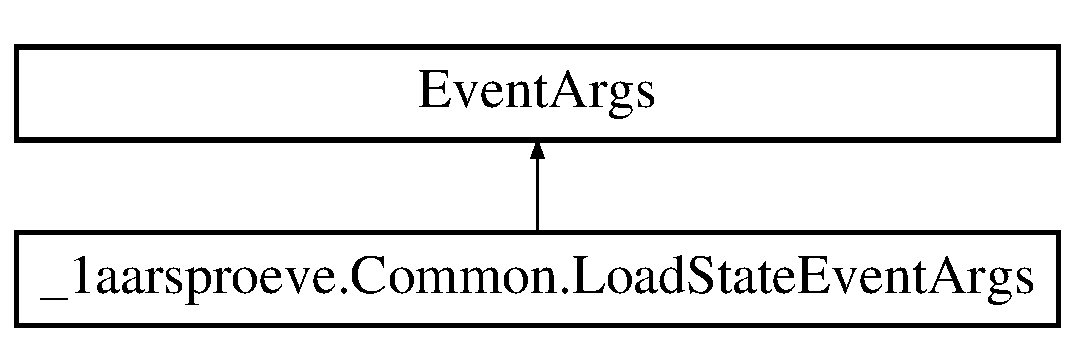
\includegraphics[height=2.000000cm]{class__1aarsproeve_1_1_common_1_1_load_state_event_args}
\end{center}
\end{figure}
\subsection*{Public Member Functions}
\begin{DoxyCompactItemize}
\item 
\hyperlink{class__1aarsproeve_1_1_common_1_1_load_state_event_args_ad17da4db8edeac5f73b571c59c6d0a0f}{Load\+State\+Event\+Args} (Object navigation\+Parameter, Dictionary$<$ string, Object $>$ page\+State)
\begin{DoxyCompactList}\small\item\em Initializes a new instance of the \hyperlink{class__1aarsproeve_1_1_common_1_1_load_state_event_args}{Load\+State\+Event\+Args} class. \end{DoxyCompactList}\end{DoxyCompactItemize}
\subsection*{Properties}
\begin{DoxyCompactItemize}
\item 
Object \hyperlink{class__1aarsproeve_1_1_common_1_1_load_state_event_args_a644716fac854626a88aa069be7987842}{Navigation\+Parameter}\hspace{0.3cm}{\ttfamily  \mbox{[}get\mbox{]}}
\begin{DoxyCompactList}\small\item\em The parameter value passed to Frame.\+Navigate(\+Type, Object) when this page was initially requested. \end{DoxyCompactList}\item 
Dictionary$<$ string, Object $>$ \hyperlink{class__1aarsproeve_1_1_common_1_1_load_state_event_args_a4578acd8233a23b822bd76aae343b720}{Page\+State}\hspace{0.3cm}{\ttfamily  \mbox{[}get\mbox{]}}
\begin{DoxyCompactList}\small\item\em A dictionary of state preserved by this page during an earlier session. This will be null the first time a page is visited. \end{DoxyCompactList}\end{DoxyCompactItemize}


\subsection{Detailed Description}
Class used to hold the event data required when a page attempts to load state. 



\subsection{Constructor \& Destructor Documentation}
\hypertarget{class__1aarsproeve_1_1_common_1_1_load_state_event_args_ad17da4db8edeac5f73b571c59c6d0a0f}{}\index{\+\_\+1aarsproeve\+::\+Common\+::\+Load\+State\+Event\+Args@{\+\_\+1aarsproeve\+::\+Common\+::\+Load\+State\+Event\+Args}!Load\+State\+Event\+Args@{Load\+State\+Event\+Args}}
\index{Load\+State\+Event\+Args@{Load\+State\+Event\+Args}!\+\_\+1aarsproeve\+::\+Common\+::\+Load\+State\+Event\+Args@{\+\_\+1aarsproeve\+::\+Common\+::\+Load\+State\+Event\+Args}}
\subsubsection[{Load\+State\+Event\+Args}]{\setlength{\rightskip}{0pt plus 5cm}\+\_\+1aarsproeve.\+Common.\+Load\+State\+Event\+Args.\+Load\+State\+Event\+Args (
\begin{DoxyParamCaption}
\item[{Object}]{navigation\+Parameter, }
\item[{Dictionary$<$ string, Object $>$}]{page\+State}
\end{DoxyParamCaption}
)}\label{class__1aarsproeve_1_1_common_1_1_load_state_event_args_ad17da4db8edeac5f73b571c59c6d0a0f}


Initializes a new instance of the \hyperlink{class__1aarsproeve_1_1_common_1_1_load_state_event_args}{Load\+State\+Event\+Args} class. 


\begin{DoxyParams}{Parameters}
{\em navigation\+Parameter} & The parameter value passed to Frame.\+Navigate(\+Type, Object) when this page was initially requested. \\
\hline
{\em page\+State} & A dictionary of state preserved by this page during an earlier session. This will be null the first time a page is visited. \\
\hline
\end{DoxyParams}


\subsection{Property Documentation}
\hypertarget{class__1aarsproeve_1_1_common_1_1_load_state_event_args_a644716fac854626a88aa069be7987842}{}\index{\+\_\+1aarsproeve\+::\+Common\+::\+Load\+State\+Event\+Args@{\+\_\+1aarsproeve\+::\+Common\+::\+Load\+State\+Event\+Args}!Navigation\+Parameter@{Navigation\+Parameter}}
\index{Navigation\+Parameter@{Navigation\+Parameter}!\+\_\+1aarsproeve\+::\+Common\+::\+Load\+State\+Event\+Args@{\+\_\+1aarsproeve\+::\+Common\+::\+Load\+State\+Event\+Args}}
\subsubsection[{Navigation\+Parameter}]{\setlength{\rightskip}{0pt plus 5cm}Object \+\_\+1aarsproeve.\+Common.\+Load\+State\+Event\+Args.\+Navigation\+Parameter\hspace{0.3cm}{\ttfamily [get]}}\label{class__1aarsproeve_1_1_common_1_1_load_state_event_args_a644716fac854626a88aa069be7987842}


The parameter value passed to Frame.\+Navigate(\+Type, Object) when this page was initially requested. 

\hypertarget{class__1aarsproeve_1_1_common_1_1_load_state_event_args_a4578acd8233a23b822bd76aae343b720}{}\index{\+\_\+1aarsproeve\+::\+Common\+::\+Load\+State\+Event\+Args@{\+\_\+1aarsproeve\+::\+Common\+::\+Load\+State\+Event\+Args}!Page\+State@{Page\+State}}
\index{Page\+State@{Page\+State}!\+\_\+1aarsproeve\+::\+Common\+::\+Load\+State\+Event\+Args@{\+\_\+1aarsproeve\+::\+Common\+::\+Load\+State\+Event\+Args}}
\subsubsection[{Page\+State}]{\setlength{\rightskip}{0pt plus 5cm}Dictionary$<$string, Object$>$ \+\_\+1aarsproeve.\+Common.\+Load\+State\+Event\+Args.\+Page\+State\hspace{0.3cm}{\ttfamily [get]}}\label{class__1aarsproeve_1_1_common_1_1_load_state_event_args_a4578acd8233a23b822bd76aae343b720}


A dictionary of state preserved by this page during an earlier session. This will be null the first time a page is visited. 



The documentation for this class was generated from the following file\+:\begin{DoxyCompactItemize}
\item 
Documents/\+Git\+Hub/1-\/aarsproeve/1aarsproeve/1aarsproeve/\+Common/Navigation\+Helper.\+cs\end{DoxyCompactItemize}

\hypertarget{class__1aarsproeve_1_1_view_1_1_login}{}\section{\+\_\+1aarsproeve.\+View.\+Login Class Reference}
\label{class__1aarsproeve_1_1_view_1_1_login}\index{\+\_\+1aarsproeve.\+View.\+Login@{\+\_\+1aarsproeve.\+View.\+Login}}


A basic page that provides characteristics common to most applications.  


Inheritance diagram for \+\_\+1aarsproeve.\+View.\+Login\+:\begin{figure}[H]
\begin{center}
\leavevmode
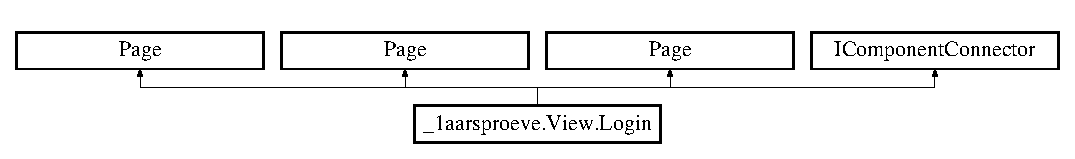
\includegraphics[height=1.686747cm]{class__1aarsproeve_1_1_view_1_1_login}
\end{center}
\end{figure}
\subsection*{Public Member Functions}
\begin{DoxyCompactItemize}
\item 
\hypertarget{class__1aarsproeve_1_1_view_1_1_login_a0b650feb728bff84ba4920865ebeffcd}{}void {\bfseries Connect} (int connection\+Id, object target)\label{class__1aarsproeve_1_1_view_1_1_login_a0b650feb728bff84ba4920865ebeffcd}

\item 
\hypertarget{class__1aarsproeve_1_1_view_1_1_login_a83c979a31b4606a57f03d1f9d095146f}{}void {\bfseries Initialize\+Component} ()\label{class__1aarsproeve_1_1_view_1_1_login_a83c979a31b4606a57f03d1f9d095146f}

\end{DoxyCompactItemize}
\subsection*{Protected Member Functions}
\begin{DoxyCompactItemize}
\item 
override void \hyperlink{class__1aarsproeve_1_1_view_1_1_login_a1d8445503157d81e1f1c70067f83e05a}{On\+Navigated\+To} (Navigation\+Event\+Args e)
\item 
\hypertarget{class__1aarsproeve_1_1_view_1_1_login_a6d48da78661aa250f8737da036c25d15}{}override void {\bfseries On\+Navigated\+From} (Navigation\+Event\+Args e)\label{class__1aarsproeve_1_1_view_1_1_login_a6d48da78661aa250f8737da036c25d15}

\end{DoxyCompactItemize}
\subsection*{Properties}
\begin{DoxyCompactItemize}
\item 
\hyperlink{class__1aarsproeve_1_1_common_1_1_observable_dictionary}{Observable\+Dictionary} \hyperlink{class__1aarsproeve_1_1_view_1_1_login_a7955bd79c353b1dcdcfcd7b73874b0a6}{Default\+View\+Model}\hspace{0.3cm}{\ttfamily  \mbox{[}get\mbox{]}}
\begin{DoxyCompactList}\small\item\em This can be changed to a strongly typed view model. \end{DoxyCompactList}\item 
\hyperlink{class__1aarsproeve_1_1_common_1_1_navigation_helper}{Navigation\+Helper} \hyperlink{class__1aarsproeve_1_1_view_1_1_login_a6ce27e4b6c4ba6f4785c2d98d4685477}{Navigation\+Helper}\hspace{0.3cm}{\ttfamily  \mbox{[}get\mbox{]}}
\begin{DoxyCompactList}\small\item\em Navigation\+Helper is used on each page to aid in navigation and process lifetime management \end{DoxyCompactList}\end{DoxyCompactItemize}


\subsection{Detailed Description}
A basic page that provides characteristics common to most applications. 



\subsection{Member Function Documentation}
\hypertarget{class__1aarsproeve_1_1_view_1_1_login_a1d8445503157d81e1f1c70067f83e05a}{}\index{\+\_\+1aarsproeve\+::\+View\+::\+Login@{\+\_\+1aarsproeve\+::\+View\+::\+Login}!On\+Navigated\+To@{On\+Navigated\+To}}
\index{On\+Navigated\+To@{On\+Navigated\+To}!\+\_\+1aarsproeve\+::\+View\+::\+Login@{\+\_\+1aarsproeve\+::\+View\+::\+Login}}
\subsubsection[{On\+Navigated\+To}]{\setlength{\rightskip}{0pt plus 5cm}override void \+\_\+1aarsproeve.\+View.\+Login.\+On\+Navigated\+To (
\begin{DoxyParamCaption}
\item[{Navigation\+Event\+Args}]{e}
\end{DoxyParamCaption}
)\hspace{0.3cm}{\ttfamily [inline]}, {\ttfamily [protected]}}\label{class__1aarsproeve_1_1_view_1_1_login_a1d8445503157d81e1f1c70067f83e05a}
The methods provided in this section are simply used to allow Navigation\+Helper to respond to the page\textquotesingle{}s navigation methods.

Page specific logic should be placed in event handlers for the Grid\+C\+S.\+Common.\+Navigation\+Helper.\+Load\+State and Grid\+C\+S.\+Common.\+Navigation\+Helper.\+Save\+State. The navigation parameter is available in the Load\+State method in addition to page state preserved during an earlier session. 

\subsection{Property Documentation}
\hypertarget{class__1aarsproeve_1_1_view_1_1_login_a7955bd79c353b1dcdcfcd7b73874b0a6}{}\index{\+\_\+1aarsproeve\+::\+View\+::\+Login@{\+\_\+1aarsproeve\+::\+View\+::\+Login}!Default\+View\+Model@{Default\+View\+Model}}
\index{Default\+View\+Model@{Default\+View\+Model}!\+\_\+1aarsproeve\+::\+View\+::\+Login@{\+\_\+1aarsproeve\+::\+View\+::\+Login}}
\subsubsection[{Default\+View\+Model}]{\setlength{\rightskip}{0pt plus 5cm}{\bf Observable\+Dictionary} \+\_\+1aarsproeve.\+View.\+Login.\+Default\+View\+Model\hspace{0.3cm}{\ttfamily [get]}}\label{class__1aarsproeve_1_1_view_1_1_login_a7955bd79c353b1dcdcfcd7b73874b0a6}


This can be changed to a strongly typed view model. 

\hypertarget{class__1aarsproeve_1_1_view_1_1_login_a6ce27e4b6c4ba6f4785c2d98d4685477}{}\index{\+\_\+1aarsproeve\+::\+View\+::\+Login@{\+\_\+1aarsproeve\+::\+View\+::\+Login}!Navigation\+Helper@{Navigation\+Helper}}
\index{Navigation\+Helper@{Navigation\+Helper}!\+\_\+1aarsproeve\+::\+View\+::\+Login@{\+\_\+1aarsproeve\+::\+View\+::\+Login}}
\subsubsection[{Navigation\+Helper}]{\setlength{\rightskip}{0pt plus 5cm}{\bf Navigation\+Helper} \+\_\+1aarsproeve.\+View.\+Login.\+Navigation\+Helper\hspace{0.3cm}{\ttfamily [get]}}\label{class__1aarsproeve_1_1_view_1_1_login_a6ce27e4b6c4ba6f4785c2d98d4685477}


Navigation\+Helper is used on each page to aid in navigation and process lifetime management 



The documentation for this class was generated from the following files\+:\begin{DoxyCompactItemize}
\item 
C\+:/\+Users/\+Daniel\+Winther/\+Documents/\+Git\+Hub/1-\/aarsproeve/1aarsproeve/1aarsproeve/obj/\+Debug/\+View/Login.\+g.\+cs\item 
C\+:/\+Users/\+Daniel\+Winther/\+Documents/\+Git\+Hub/1-\/aarsproeve/1aarsproeve/1aarsproeve/obj/\+Debug/\+View/Login.\+g.\+i.\+cs\item 
C\+:/\+Users/\+Daniel\+Winther/\+Documents/\+Git\+Hub/1-\/aarsproeve/1aarsproeve/1aarsproeve/\+View/Login.\+xaml.\+cs\end{DoxyCompactItemize}

\hypertarget{class__1aarsproeve_1_1_main_page}{}\section{\+\_\+1aarsproeve.\+Main\+Page Class Reference}
\label{class__1aarsproeve_1_1_main_page}\index{\+\_\+1aarsproeve.\+Main\+Page@{\+\_\+1aarsproeve.\+Main\+Page}}
Inheritance diagram for \+\_\+1aarsproeve.\+Main\+Page\+:\begin{figure}[H]
\begin{center}
\leavevmode
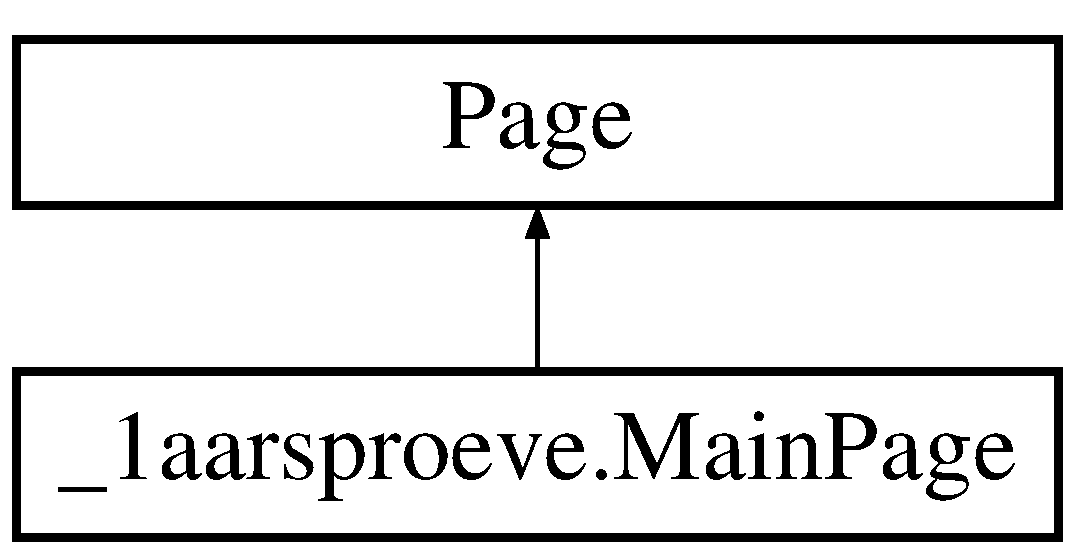
\includegraphics[height=2.000000cm]{class__1aarsproeve_1_1_main_page}
\end{center}
\end{figure}
\subsection*{Public Member Functions}
\begin{DoxyCompactItemize}
\item 
\hypertarget{class__1aarsproeve_1_1_main_page_a894e5b8cbf318b168cecd11961976ccf}{}void {\bfseries Initialize\+Component} ()\label{class__1aarsproeve_1_1_main_page_a894e5b8cbf318b168cecd11961976ccf}

\end{DoxyCompactItemize}


The documentation for this class was generated from the following file\+:\begin{DoxyCompactItemize}
\item 
Documents/\+Git\+Hub/1-\/aarsproeve/1aarsproeve/1aarsproeve/obj/\+Debug/\+View/Main\+Page.\+g.\+i.\+cs\end{DoxyCompactItemize}

\hypertarget{class__1aarsproeve_web_service_1_1_areas_1_1_help_page_1_1_model_descriptions_1_1_model_description}{}\section{\+\_\+1aarsproeve\+Web\+Service.\+Areas.\+Help\+Page.\+Model\+Descriptions.\+Model\+Description Class Reference}
\label{class__1aarsproeve_web_service_1_1_areas_1_1_help_page_1_1_model_descriptions_1_1_model_description}\index{\+\_\+1aarsproeve\+Web\+Service.\+Areas.\+Help\+Page.\+Model\+Descriptions.\+Model\+Description@{\+\_\+1aarsproeve\+Web\+Service.\+Areas.\+Help\+Page.\+Model\+Descriptions.\+Model\+Description}}


Describes a type model.  


Inheritance diagram for \+\_\+1aarsproeve\+Web\+Service.\+Areas.\+Help\+Page.\+Model\+Descriptions.\+Model\+Description\+:\begin{figure}[H]
\begin{center}
\leavevmode
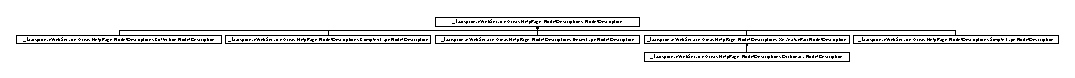
\includegraphics[height=0.605405cm]{class__1aarsproeve_web_service_1_1_areas_1_1_help_page_1_1_model_descriptions_1_1_model_description}
\end{center}
\end{figure}
\subsection*{Properties}
\begin{DoxyCompactItemize}
\item 
\hypertarget{class__1aarsproeve_web_service_1_1_areas_1_1_help_page_1_1_model_descriptions_1_1_model_description_ac4829682ab8e3a3dd80316cecbf26005}{}string {\bfseries Documentation}\hspace{0.3cm}{\ttfamily  \mbox{[}get, set\mbox{]}}\label{class__1aarsproeve_web_service_1_1_areas_1_1_help_page_1_1_model_descriptions_1_1_model_description_ac4829682ab8e3a3dd80316cecbf26005}

\item 
\hypertarget{class__1aarsproeve_web_service_1_1_areas_1_1_help_page_1_1_model_descriptions_1_1_model_description_a33288a937777275fb9acd1b2befdf541}{}Type {\bfseries Model\+Type}\hspace{0.3cm}{\ttfamily  \mbox{[}get, set\mbox{]}}\label{class__1aarsproeve_web_service_1_1_areas_1_1_help_page_1_1_model_descriptions_1_1_model_description_a33288a937777275fb9acd1b2befdf541}

\item 
\hypertarget{class__1aarsproeve_web_service_1_1_areas_1_1_help_page_1_1_model_descriptions_1_1_model_description_ae243f1257accc1f9e2809fc21dccad60}{}string {\bfseries Name}\hspace{0.3cm}{\ttfamily  \mbox{[}get, set\mbox{]}}\label{class__1aarsproeve_web_service_1_1_areas_1_1_help_page_1_1_model_descriptions_1_1_model_description_ae243f1257accc1f9e2809fc21dccad60}

\end{DoxyCompactItemize}


\subsection{Detailed Description}
Describes a type model. 



The documentation for this class was generated from the following file\+:\begin{DoxyCompactItemize}
\item 
Documents/\+Git\+Hub/1-\/aarsproeve/1aarsproeve/1aarsproeve\+Web\+Service/\+Areas/\+Help\+Page/\+Model\+Descriptions/Model\+Description.\+cs\end{DoxyCompactItemize}

\hypertarget{class__1aarsproeve_web_service_1_1_areas_1_1_help_page_1_1_model_descriptions_1_1_model_description_generator}{}\section{\+\_\+1aarsproeve\+Web\+Service.\+Areas.\+Help\+Page.\+Model\+Descriptions.\+Model\+Description\+Generator Class Reference}
\label{class__1aarsproeve_web_service_1_1_areas_1_1_help_page_1_1_model_descriptions_1_1_model_description_generator}\index{\+\_\+1aarsproeve\+Web\+Service.\+Areas.\+Help\+Page.\+Model\+Descriptions.\+Model\+Description\+Generator@{\+\_\+1aarsproeve\+Web\+Service.\+Areas.\+Help\+Page.\+Model\+Descriptions.\+Model\+Description\+Generator}}


Generates model descriptions for given types.  


\subsection*{Public Member Functions}
\begin{DoxyCompactItemize}
\item 
\hypertarget{class__1aarsproeve_web_service_1_1_areas_1_1_help_page_1_1_model_descriptions_1_1_model_description_generator_a0f18212af9433afee89acbe3cc8de6be}{}{\bfseries Model\+Description\+Generator} (Http\+Configuration config)\label{class__1aarsproeve_web_service_1_1_areas_1_1_help_page_1_1_model_descriptions_1_1_model_description_generator_a0f18212af9433afee89acbe3cc8de6be}

\item 
\hypertarget{class__1aarsproeve_web_service_1_1_areas_1_1_help_page_1_1_model_descriptions_1_1_model_description_generator_a9404c6e00ceee0f3eee2301f975d15ab}{}\hyperlink{class__1aarsproeve_web_service_1_1_areas_1_1_help_page_1_1_model_descriptions_1_1_model_description}{Model\+Description} {\bfseries Get\+Or\+Create\+Model\+Description} (Type model\+Type)\label{class__1aarsproeve_web_service_1_1_areas_1_1_help_page_1_1_model_descriptions_1_1_model_description_generator_a9404c6e00ceee0f3eee2301f975d15ab}

\end{DoxyCompactItemize}
\subsection*{Properties}
\begin{DoxyCompactItemize}
\item 
\hypertarget{class__1aarsproeve_web_service_1_1_areas_1_1_help_page_1_1_model_descriptions_1_1_model_description_generator_a9a3ccc6d1bf37f5189f07f2a044568bb}{}Dictionary$<$ string, \hyperlink{class__1aarsproeve_web_service_1_1_areas_1_1_help_page_1_1_model_descriptions_1_1_model_description}{Model\+Description} $>$ {\bfseries Generated\+Models}\hspace{0.3cm}{\ttfamily  \mbox{[}get\mbox{]}}\label{class__1aarsproeve_web_service_1_1_areas_1_1_help_page_1_1_model_descriptions_1_1_model_description_generator_a9a3ccc6d1bf37f5189f07f2a044568bb}

\end{DoxyCompactItemize}


\subsection{Detailed Description}
Generates model descriptions for given types. 



The documentation for this class was generated from the following file\+:\begin{DoxyCompactItemize}
\item 
C\+:/\+Users/\+Daniel\+Winther/\+Documents/\+Git\+Hub/1-\/aarsproeve/1aarsproeve/1aarsproeve\+Web\+Service/\+Areas/\+Help\+Page/\+Model\+Descriptions/Model\+Description\+Generator.\+cs\end{DoxyCompactItemize}

\hypertarget{class__1aarsproeve_web_service_1_1_areas_1_1_help_page_1_1_model_descriptions_1_1_model_name_attribute}{}\section{\+\_\+1aarsproeve\+Web\+Service.\+Areas.\+Help\+Page.\+Model\+Descriptions.\+Model\+Name\+Attribute Class Reference}
\label{class__1aarsproeve_web_service_1_1_areas_1_1_help_page_1_1_model_descriptions_1_1_model_name_attribute}\index{\+\_\+1aarsproeve\+Web\+Service.\+Areas.\+Help\+Page.\+Model\+Descriptions.\+Model\+Name\+Attribute@{\+\_\+1aarsproeve\+Web\+Service.\+Areas.\+Help\+Page.\+Model\+Descriptions.\+Model\+Name\+Attribute}}


Use this attribute to change the name of the \hyperlink{class__1aarsproeve_web_service_1_1_areas_1_1_help_page_1_1_model_descriptions_1_1_model_description}{Model\+Description} generated for a type.  


Inheritance diagram for \+\_\+1aarsproeve\+Web\+Service.\+Areas.\+Help\+Page.\+Model\+Descriptions.\+Model\+Name\+Attribute\+:\begin{figure}[H]
\begin{center}
\leavevmode
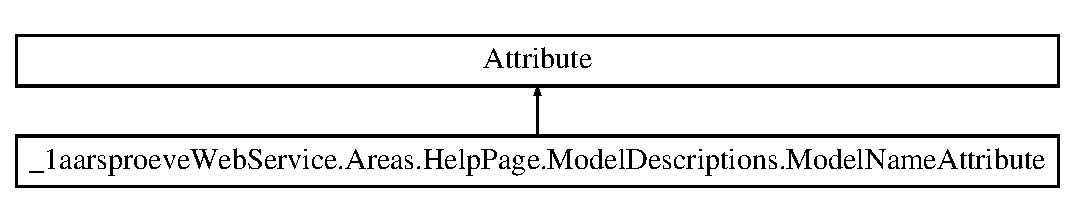
\includegraphics[height=2.000000cm]{class__1aarsproeve_web_service_1_1_areas_1_1_help_page_1_1_model_descriptions_1_1_model_name_attribute}
\end{center}
\end{figure}
\subsection*{Public Member Functions}
\begin{DoxyCompactItemize}
\item 
\hypertarget{class__1aarsproeve_web_service_1_1_areas_1_1_help_page_1_1_model_descriptions_1_1_model_name_attribute_a3c556da4a2c88b8dd1f01756a0d66295}{}{\bfseries Model\+Name\+Attribute} (string name)\label{class__1aarsproeve_web_service_1_1_areas_1_1_help_page_1_1_model_descriptions_1_1_model_name_attribute_a3c556da4a2c88b8dd1f01756a0d66295}

\end{DoxyCompactItemize}
\subsection*{Properties}
\begin{DoxyCompactItemize}
\item 
\hypertarget{class__1aarsproeve_web_service_1_1_areas_1_1_help_page_1_1_model_descriptions_1_1_model_name_attribute_afe346b943d7fc65f710a10b44173dc57}{}string {\bfseries Name}\hspace{0.3cm}{\ttfamily  \mbox{[}get\mbox{]}}\label{class__1aarsproeve_web_service_1_1_areas_1_1_help_page_1_1_model_descriptions_1_1_model_name_attribute_afe346b943d7fc65f710a10b44173dc57}

\end{DoxyCompactItemize}


\subsection{Detailed Description}
Use this attribute to change the name of the \hyperlink{class__1aarsproeve_web_service_1_1_areas_1_1_help_page_1_1_model_descriptions_1_1_model_description}{Model\+Description} generated for a type. 



The documentation for this class was generated from the following file\+:\begin{DoxyCompactItemize}
\item 
C\+:/\+Users/\+Daniel\+Winther/\+Documents/\+Git\+Hub/1-\/aarsproeve/1aarsproeve/1aarsproeve\+Web\+Service/\+Areas/\+Help\+Page/\+Model\+Descriptions/Model\+Name\+Attribute.\+cs\end{DoxyCompactItemize}

\hypertarget{class__1aarsproeve_1_1_common_1_1_navigation_helper}{}\section{\+\_\+1aarsproeve.\+Common.\+Navigation\+Helper Class Reference}
\label{class__1aarsproeve_1_1_common_1_1_navigation_helper}\index{\+\_\+1aarsproeve.\+Common.\+Navigation\+Helper@{\+\_\+1aarsproeve.\+Common.\+Navigation\+Helper}}


\hyperlink{class__1aarsproeve_1_1_common_1_1_navigation_helper}{Navigation\+Helper} aids in navigation between pages. It provides commands used to navigate back and forward as well as registers for standard mouse and keyboard shortcuts used to go back and forward in Windows and the hardware back button in Windows Phone. In addition it integrates Suspension\+Manger to handle process lifetime management and state management when navigating between pages.  


Inheritance diagram for \+\_\+1aarsproeve.\+Common.\+Navigation\+Helper\+:\begin{figure}[H]
\begin{center}
\leavevmode
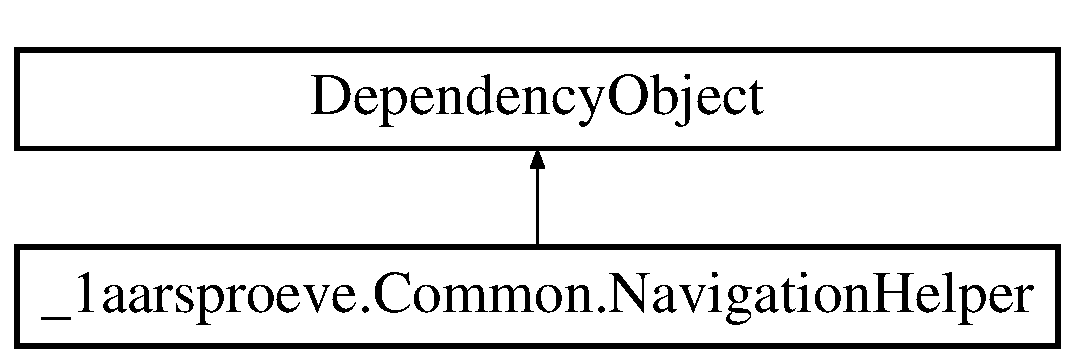
\includegraphics[height=2.000000cm]{class__1aarsproeve_1_1_common_1_1_navigation_helper}
\end{center}
\end{figure}
\subsection*{Public Member Functions}
\begin{DoxyCompactItemize}
\item 
\hyperlink{class__1aarsproeve_1_1_common_1_1_navigation_helper_af14c5526e239fb66aa413b026b555cdb}{Navigation\+Helper} (Page page)
\begin{DoxyCompactList}\small\item\em Initializes a new instance of the \hyperlink{class__1aarsproeve_1_1_common_1_1_navigation_helper}{Navigation\+Helper} class. \end{DoxyCompactList}\item 
virtual bool \hyperlink{class__1aarsproeve_1_1_common_1_1_navigation_helper_a6022d2d426e7213d412325d1b9fc05ed}{Can\+Go\+Back} ()
\begin{DoxyCompactList}\small\item\em Virtual method used by the \hyperlink{class__1aarsproeve_1_1_common_1_1_navigation_helper_a4f5f9df95a5c10434b08d04da50a2467}{Go\+Back\+Command} property to determine if the Frame can go back. \end{DoxyCompactList}\item 
virtual bool \hyperlink{class__1aarsproeve_1_1_common_1_1_navigation_helper_aaa3cbdb865a20d782eff8cd283bb8e0b}{Can\+Go\+Forward} ()
\begin{DoxyCompactList}\small\item\em Virtual method used by the \hyperlink{class__1aarsproeve_1_1_common_1_1_navigation_helper_a9bb68ebbefcf2daaeaf8f18775eb8a80}{Go\+Forward\+Command} property to determine if the Frame can go forward. \end{DoxyCompactList}\item 
virtual void \hyperlink{class__1aarsproeve_1_1_common_1_1_navigation_helper_ac31589f6f0725544c6d6f8c409816a9c}{Go\+Back} ()
\begin{DoxyCompactList}\small\item\em Virtual method used by the \hyperlink{class__1aarsproeve_1_1_common_1_1_navigation_helper_a4f5f9df95a5c10434b08d04da50a2467}{Go\+Back\+Command} property to invoke the Windows.\+U\+I.\+Xaml.\+Controls.\+Frame.\+Go\+Back method. \end{DoxyCompactList}\item 
virtual void \hyperlink{class__1aarsproeve_1_1_common_1_1_navigation_helper_a56206b1bac5776daee0f5c79e26d4845}{Go\+Forward} ()
\begin{DoxyCompactList}\small\item\em Virtual method used by the \hyperlink{class__1aarsproeve_1_1_common_1_1_navigation_helper_a9bb68ebbefcf2daaeaf8f18775eb8a80}{Go\+Forward\+Command} property to invoke the Windows.\+U\+I.\+Xaml.\+Controls.\+Frame.\+Go\+Forward method. \end{DoxyCompactList}\item 
void \hyperlink{class__1aarsproeve_1_1_common_1_1_navigation_helper_a592295e4be4ec349fd13c6d4700e32e2}{On\+Navigated\+To} (Navigation\+Event\+Args e)
\begin{DoxyCompactList}\small\item\em Invoked when this page is about to be displayed in a Frame. This method calls \hyperlink{class__1aarsproeve_1_1_common_1_1_navigation_helper_ab4abff9d3eb04794d05d43ff3846e344}{Load\+State}, where all page specific navigation and process lifetime management logic should be placed. \end{DoxyCompactList}\item 
void \hyperlink{class__1aarsproeve_1_1_common_1_1_navigation_helper_a0919c4c25dadbd1e73ec38691a6997fe}{On\+Navigated\+From} (Navigation\+Event\+Args e)
\begin{DoxyCompactList}\small\item\em Invoked when this page will no longer be displayed in a Frame. This method calls \hyperlink{class__1aarsproeve_1_1_common_1_1_navigation_helper_a627a89278c28e536b6e7fea11da6d465}{Save\+State}, where all page specific navigation and process lifetime management logic should be placed. \end{DoxyCompactList}\end{DoxyCompactItemize}
\subsection*{Properties}
\begin{DoxyCompactItemize}
\item 
\hyperlink{class__1aarsproeve_1_1_common_1_1_relay_command}{Relay\+Command} \hyperlink{class__1aarsproeve_1_1_common_1_1_navigation_helper_a4f5f9df95a5c10434b08d04da50a2467}{Go\+Back\+Command}\hspace{0.3cm}{\ttfamily  \mbox{[}get, set\mbox{]}}
\begin{DoxyCompactList}\small\item\em \hyperlink{class__1aarsproeve_1_1_common_1_1_relay_command}{Relay\+Command} used to bind to the back Button\textquotesingle{}s Command property for navigating to the most recent item in back navigation history, if a Frame manages its own navigation history. \end{DoxyCompactList}\item 
\hyperlink{class__1aarsproeve_1_1_common_1_1_relay_command}{Relay\+Command} \hyperlink{class__1aarsproeve_1_1_common_1_1_navigation_helper_a9bb68ebbefcf2daaeaf8f18775eb8a80}{Go\+Forward\+Command}\hspace{0.3cm}{\ttfamily  \mbox{[}get\mbox{]}}
\begin{DoxyCompactList}\small\item\em \hyperlink{class__1aarsproeve_1_1_common_1_1_relay_command}{Relay\+Command} used for navigating to the most recent item in the forward navigation history, if a Frame manages its own navigation history. \end{DoxyCompactList}\end{DoxyCompactItemize}
\subsection*{Events}
\begin{DoxyCompactItemize}
\item 
\hyperlink{namespace__1aarsproeve_1_1_common_aee964a591f5ee233e54c70f38c9334cf}{Load\+State\+Event\+Handler} \hyperlink{class__1aarsproeve_1_1_common_1_1_navigation_helper_ab4abff9d3eb04794d05d43ff3846e344}{Load\+State}
\begin{DoxyCompactList}\small\item\em Register this event on the current page to populate the page with content passed during navigation as well as any saved state provided when recreating a page from a prior session. \end{DoxyCompactList}\item 
\hyperlink{namespace__1aarsproeve_1_1_common_acae0399935efb5f4aff5ba3cdfd92246}{Save\+State\+Event\+Handler} \hyperlink{class__1aarsproeve_1_1_common_1_1_navigation_helper_a627a89278c28e536b6e7fea11da6d465}{Save\+State}
\begin{DoxyCompactList}\small\item\em Register this event on the current page to preserve state associated with the current page in case the application is suspended or the page is discarded from the navigaqtion cache. \end{DoxyCompactList}\end{DoxyCompactItemize}


\subsection{Detailed Description}
\hyperlink{class__1aarsproeve_1_1_common_1_1_navigation_helper}{Navigation\+Helper} aids in navigation between pages. It provides commands used to navigate back and forward as well as registers for standard mouse and keyboard shortcuts used to go back and forward in Windows and the hardware back button in Windows Phone. In addition it integrates Suspension\+Manger to handle process lifetime management and state management when navigating between pages. 

To make use of \hyperlink{class__1aarsproeve_1_1_common_1_1_navigation_helper}{Navigation\+Helper}, follow these two steps or start with a Basic\+Page or any other Page item template other than Blank\+Page.

1) Create an instance of the \hyperlink{class__1aarsproeve_1_1_common_1_1_navigation_helper}{Navigation\+Helper} somewhere such as in the constructor for the page and register a callback for the Load\+State and Save\+State events. 
\begin{DoxyCode}
\textcolor{keyword}{public} MyPage()
\{
    this.InitializeComponent();
    var navigationHelper = \textcolor{keyword}{new} \hyperlink{class__1aarsproeve_1_1_common_1_1_navigation_helper_af14c5526e239fb66aa413b026b555cdb}{NavigationHelper}(\textcolor{keyword}{this});
    this.navigationHelper.LoadState += navigationHelper\_LoadState;
    this.navigationHelper.SaveState += navigationHelper\_SaveState;
\}

\textcolor{keyword}{private} async \textcolor{keywordtype}{void} navigationHelper\_LoadState(\textcolor{keywordtype}{object} sender, LoadStateEventArgs e)
\{ \}
\textcolor{keyword}{private} async \textcolor{keywordtype}{void} navigationHelper\_SaveState(\textcolor{keywordtype}{object} sender, LoadStateEventArgs e)
\{ \}
\end{DoxyCode}


2) Register the page to call into the \hyperlink{class__1aarsproeve_1_1_common_1_1_navigation_helper}{Navigation\+Helper} whenever the page participates in navigation by overriding the Windows.\+U\+I.\+Xaml.\+Controls.\+Page.\+On\+Navigated\+To and Windows.\+U\+I.\+Xaml.\+Controls.\+Page.\+On\+Navigated\+From events. 
\begin{DoxyCode}
\textcolor{keyword}{protected} \textcolor{keyword}{override} \textcolor{keywordtype}{void} \hyperlink{class__1aarsproeve_1_1_common_1_1_navigation_helper_a592295e4be4ec349fd13c6d4700e32e2}{OnNavigatedTo}(NavigationEventArgs e)
\{
    navigationHelper.OnNavigatedTo(e);
\}

\textcolor{keyword}{protected} \textcolor{keyword}{override} \textcolor{keywordtype}{void} \hyperlink{class__1aarsproeve_1_1_common_1_1_navigation_helper_a0919c4c25dadbd1e73ec38691a6997fe}{OnNavigatedFrom}(NavigationEventArgs e)
\{
    navigationHelper.OnNavigatedFrom(e);
\}
\end{DoxyCode}
 

\subsection{Constructor \& Destructor Documentation}
\hypertarget{class__1aarsproeve_1_1_common_1_1_navigation_helper_af14c5526e239fb66aa413b026b555cdb}{}\index{\+\_\+1aarsproeve\+::\+Common\+::\+Navigation\+Helper@{\+\_\+1aarsproeve\+::\+Common\+::\+Navigation\+Helper}!Navigation\+Helper@{Navigation\+Helper}}
\index{Navigation\+Helper@{Navigation\+Helper}!\+\_\+1aarsproeve\+::\+Common\+::\+Navigation\+Helper@{\+\_\+1aarsproeve\+::\+Common\+::\+Navigation\+Helper}}
\subsubsection[{Navigation\+Helper}]{\setlength{\rightskip}{0pt plus 5cm}\+\_\+1aarsproeve.\+Common.\+Navigation\+Helper.\+Navigation\+Helper (
\begin{DoxyParamCaption}
\item[{Page}]{page}
\end{DoxyParamCaption}
)\hspace{0.3cm}{\ttfamily [inline]}}\label{class__1aarsproeve_1_1_common_1_1_navigation_helper_af14c5526e239fb66aa413b026b555cdb}


Initializes a new instance of the \hyperlink{class__1aarsproeve_1_1_common_1_1_navigation_helper}{Navigation\+Helper} class. 


\begin{DoxyParams}{Parameters}
{\em page} & A reference to the current page used for navigation. This reference allows for frame manipulation and to ensure that keyboard navigation requests only occur when the page is occupying the entire window.\\
\hline
\end{DoxyParams}


\subsection{Member Function Documentation}
\hypertarget{class__1aarsproeve_1_1_common_1_1_navigation_helper_a6022d2d426e7213d412325d1b9fc05ed}{}\index{\+\_\+1aarsproeve\+::\+Common\+::\+Navigation\+Helper@{\+\_\+1aarsproeve\+::\+Common\+::\+Navigation\+Helper}!Can\+Go\+Back@{Can\+Go\+Back}}
\index{Can\+Go\+Back@{Can\+Go\+Back}!\+\_\+1aarsproeve\+::\+Common\+::\+Navigation\+Helper@{\+\_\+1aarsproeve\+::\+Common\+::\+Navigation\+Helper}}
\subsubsection[{Can\+Go\+Back}]{\setlength{\rightskip}{0pt plus 5cm}virtual bool \+\_\+1aarsproeve.\+Common.\+Navigation\+Helper.\+Can\+Go\+Back (
\begin{DoxyParamCaption}
{}
\end{DoxyParamCaption}
)\hspace{0.3cm}{\ttfamily [inline]}, {\ttfamily [virtual]}}\label{class__1aarsproeve_1_1_common_1_1_navigation_helper_a6022d2d426e7213d412325d1b9fc05ed}


Virtual method used by the \hyperlink{class__1aarsproeve_1_1_common_1_1_navigation_helper_a4f5f9df95a5c10434b08d04da50a2467}{Go\+Back\+Command} property to determine if the Frame can go back. 

\begin{DoxyReturn}{Returns}
true if the Frame has at least one entry in the back navigation history. 
\end{DoxyReturn}
\hypertarget{class__1aarsproeve_1_1_common_1_1_navigation_helper_aaa3cbdb865a20d782eff8cd283bb8e0b}{}\index{\+\_\+1aarsproeve\+::\+Common\+::\+Navigation\+Helper@{\+\_\+1aarsproeve\+::\+Common\+::\+Navigation\+Helper}!Can\+Go\+Forward@{Can\+Go\+Forward}}
\index{Can\+Go\+Forward@{Can\+Go\+Forward}!\+\_\+1aarsproeve\+::\+Common\+::\+Navigation\+Helper@{\+\_\+1aarsproeve\+::\+Common\+::\+Navigation\+Helper}}
\subsubsection[{Can\+Go\+Forward}]{\setlength{\rightskip}{0pt plus 5cm}virtual bool \+\_\+1aarsproeve.\+Common.\+Navigation\+Helper.\+Can\+Go\+Forward (
\begin{DoxyParamCaption}
{}
\end{DoxyParamCaption}
)\hspace{0.3cm}{\ttfamily [inline]}, {\ttfamily [virtual]}}\label{class__1aarsproeve_1_1_common_1_1_navigation_helper_aaa3cbdb865a20d782eff8cd283bb8e0b}


Virtual method used by the \hyperlink{class__1aarsproeve_1_1_common_1_1_navigation_helper_a9bb68ebbefcf2daaeaf8f18775eb8a80}{Go\+Forward\+Command} property to determine if the Frame can go forward. 

\begin{DoxyReturn}{Returns}
true if the Frame has at least one entry in the forward navigation history. 
\end{DoxyReturn}
\hypertarget{class__1aarsproeve_1_1_common_1_1_navigation_helper_ac31589f6f0725544c6d6f8c409816a9c}{}\index{\+\_\+1aarsproeve\+::\+Common\+::\+Navigation\+Helper@{\+\_\+1aarsproeve\+::\+Common\+::\+Navigation\+Helper}!Go\+Back@{Go\+Back}}
\index{Go\+Back@{Go\+Back}!\+\_\+1aarsproeve\+::\+Common\+::\+Navigation\+Helper@{\+\_\+1aarsproeve\+::\+Common\+::\+Navigation\+Helper}}
\subsubsection[{Go\+Back}]{\setlength{\rightskip}{0pt plus 5cm}virtual void \+\_\+1aarsproeve.\+Common.\+Navigation\+Helper.\+Go\+Back (
\begin{DoxyParamCaption}
{}
\end{DoxyParamCaption}
)\hspace{0.3cm}{\ttfamily [inline]}, {\ttfamily [virtual]}}\label{class__1aarsproeve_1_1_common_1_1_navigation_helper_ac31589f6f0725544c6d6f8c409816a9c}


Virtual method used by the \hyperlink{class__1aarsproeve_1_1_common_1_1_navigation_helper_a4f5f9df95a5c10434b08d04da50a2467}{Go\+Back\+Command} property to invoke the Windows.\+U\+I.\+Xaml.\+Controls.\+Frame.\+Go\+Back method. 

\hypertarget{class__1aarsproeve_1_1_common_1_1_navigation_helper_a56206b1bac5776daee0f5c79e26d4845}{}\index{\+\_\+1aarsproeve\+::\+Common\+::\+Navigation\+Helper@{\+\_\+1aarsproeve\+::\+Common\+::\+Navigation\+Helper}!Go\+Forward@{Go\+Forward}}
\index{Go\+Forward@{Go\+Forward}!\+\_\+1aarsproeve\+::\+Common\+::\+Navigation\+Helper@{\+\_\+1aarsproeve\+::\+Common\+::\+Navigation\+Helper}}
\subsubsection[{Go\+Forward}]{\setlength{\rightskip}{0pt plus 5cm}virtual void \+\_\+1aarsproeve.\+Common.\+Navigation\+Helper.\+Go\+Forward (
\begin{DoxyParamCaption}
{}
\end{DoxyParamCaption}
)\hspace{0.3cm}{\ttfamily [inline]}, {\ttfamily [virtual]}}\label{class__1aarsproeve_1_1_common_1_1_navigation_helper_a56206b1bac5776daee0f5c79e26d4845}


Virtual method used by the \hyperlink{class__1aarsproeve_1_1_common_1_1_navigation_helper_a9bb68ebbefcf2daaeaf8f18775eb8a80}{Go\+Forward\+Command} property to invoke the Windows.\+U\+I.\+Xaml.\+Controls.\+Frame.\+Go\+Forward method. 

\hypertarget{class__1aarsproeve_1_1_common_1_1_navigation_helper_a0919c4c25dadbd1e73ec38691a6997fe}{}\index{\+\_\+1aarsproeve\+::\+Common\+::\+Navigation\+Helper@{\+\_\+1aarsproeve\+::\+Common\+::\+Navigation\+Helper}!On\+Navigated\+From@{On\+Navigated\+From}}
\index{On\+Navigated\+From@{On\+Navigated\+From}!\+\_\+1aarsproeve\+::\+Common\+::\+Navigation\+Helper@{\+\_\+1aarsproeve\+::\+Common\+::\+Navigation\+Helper}}
\subsubsection[{On\+Navigated\+From}]{\setlength{\rightskip}{0pt plus 5cm}void \+\_\+1aarsproeve.\+Common.\+Navigation\+Helper.\+On\+Navigated\+From (
\begin{DoxyParamCaption}
\item[{Navigation\+Event\+Args}]{e}
\end{DoxyParamCaption}
)\hspace{0.3cm}{\ttfamily [inline]}}\label{class__1aarsproeve_1_1_common_1_1_navigation_helper_a0919c4c25dadbd1e73ec38691a6997fe}


Invoked when this page will no longer be displayed in a Frame. This method calls \hyperlink{class__1aarsproeve_1_1_common_1_1_navigation_helper_a627a89278c28e536b6e7fea11da6d465}{Save\+State}, where all page specific navigation and process lifetime management logic should be placed. 


\begin{DoxyParams}{Parameters}
{\em e} & Event data that describes how this page was reached. The Parameter property provides the group to be displayed.\\
\hline
\end{DoxyParams}
\hypertarget{class__1aarsproeve_1_1_common_1_1_navigation_helper_a592295e4be4ec349fd13c6d4700e32e2}{}\index{\+\_\+1aarsproeve\+::\+Common\+::\+Navigation\+Helper@{\+\_\+1aarsproeve\+::\+Common\+::\+Navigation\+Helper}!On\+Navigated\+To@{On\+Navigated\+To}}
\index{On\+Navigated\+To@{On\+Navigated\+To}!\+\_\+1aarsproeve\+::\+Common\+::\+Navigation\+Helper@{\+\_\+1aarsproeve\+::\+Common\+::\+Navigation\+Helper}}
\subsubsection[{On\+Navigated\+To}]{\setlength{\rightskip}{0pt plus 5cm}void \+\_\+1aarsproeve.\+Common.\+Navigation\+Helper.\+On\+Navigated\+To (
\begin{DoxyParamCaption}
\item[{Navigation\+Event\+Args}]{e}
\end{DoxyParamCaption}
)\hspace{0.3cm}{\ttfamily [inline]}}\label{class__1aarsproeve_1_1_common_1_1_navigation_helper_a592295e4be4ec349fd13c6d4700e32e2}


Invoked when this page is about to be displayed in a Frame. This method calls \hyperlink{class__1aarsproeve_1_1_common_1_1_navigation_helper_ab4abff9d3eb04794d05d43ff3846e344}{Load\+State}, where all page specific navigation and process lifetime management logic should be placed. 


\begin{DoxyParams}{Parameters}
{\em e} & Event data that describes how this page was reached. The Parameter property provides the group to be displayed.\\
\hline
\end{DoxyParams}


\subsection{Property Documentation}
\hypertarget{class__1aarsproeve_1_1_common_1_1_navigation_helper_a4f5f9df95a5c10434b08d04da50a2467}{}\index{\+\_\+1aarsproeve\+::\+Common\+::\+Navigation\+Helper@{\+\_\+1aarsproeve\+::\+Common\+::\+Navigation\+Helper}!Go\+Back\+Command@{Go\+Back\+Command}}
\index{Go\+Back\+Command@{Go\+Back\+Command}!\+\_\+1aarsproeve\+::\+Common\+::\+Navigation\+Helper@{\+\_\+1aarsproeve\+::\+Common\+::\+Navigation\+Helper}}
\subsubsection[{Go\+Back\+Command}]{\setlength{\rightskip}{0pt plus 5cm}{\bf Relay\+Command} \+\_\+1aarsproeve.\+Common.\+Navigation\+Helper.\+Go\+Back\+Command\hspace{0.3cm}{\ttfamily [get]}, {\ttfamily [set]}}\label{class__1aarsproeve_1_1_common_1_1_navigation_helper_a4f5f9df95a5c10434b08d04da50a2467}


\hyperlink{class__1aarsproeve_1_1_common_1_1_relay_command}{Relay\+Command} used to bind to the back Button\textquotesingle{}s Command property for navigating to the most recent item in back navigation history, if a Frame manages its own navigation history. 

The \hyperlink{class__1aarsproeve_1_1_common_1_1_relay_command}{Relay\+Command} is set up to use the virtual method \hyperlink{class__1aarsproeve_1_1_common_1_1_navigation_helper_ac31589f6f0725544c6d6f8c409816a9c}{Go\+Back} as the Execute Action and \hyperlink{class__1aarsproeve_1_1_common_1_1_navigation_helper_a6022d2d426e7213d412325d1b9fc05ed}{Can\+Go\+Back} for Can\+Execute. \hypertarget{class__1aarsproeve_1_1_common_1_1_navigation_helper_a9bb68ebbefcf2daaeaf8f18775eb8a80}{}\index{\+\_\+1aarsproeve\+::\+Common\+::\+Navigation\+Helper@{\+\_\+1aarsproeve\+::\+Common\+::\+Navigation\+Helper}!Go\+Forward\+Command@{Go\+Forward\+Command}}
\index{Go\+Forward\+Command@{Go\+Forward\+Command}!\+\_\+1aarsproeve\+::\+Common\+::\+Navigation\+Helper@{\+\_\+1aarsproeve\+::\+Common\+::\+Navigation\+Helper}}
\subsubsection[{Go\+Forward\+Command}]{\setlength{\rightskip}{0pt plus 5cm}{\bf Relay\+Command} \+\_\+1aarsproeve.\+Common.\+Navigation\+Helper.\+Go\+Forward\+Command\hspace{0.3cm}{\ttfamily [get]}}\label{class__1aarsproeve_1_1_common_1_1_navigation_helper_a9bb68ebbefcf2daaeaf8f18775eb8a80}


\hyperlink{class__1aarsproeve_1_1_common_1_1_relay_command}{Relay\+Command} used for navigating to the most recent item in the forward navigation history, if a Frame manages its own navigation history. 

The \hyperlink{class__1aarsproeve_1_1_common_1_1_relay_command}{Relay\+Command} is set up to use the virtual method \hyperlink{class__1aarsproeve_1_1_common_1_1_navigation_helper_a56206b1bac5776daee0f5c79e26d4845}{Go\+Forward} as the Execute Action and \hyperlink{class__1aarsproeve_1_1_common_1_1_navigation_helper_aaa3cbdb865a20d782eff8cd283bb8e0b}{Can\+Go\+Forward} for Can\+Execute. 

\subsection{Event Documentation}
\hypertarget{class__1aarsproeve_1_1_common_1_1_navigation_helper_ab4abff9d3eb04794d05d43ff3846e344}{}\index{\+\_\+1aarsproeve\+::\+Common\+::\+Navigation\+Helper@{\+\_\+1aarsproeve\+::\+Common\+::\+Navigation\+Helper}!Load\+State@{Load\+State}}
\index{Load\+State@{Load\+State}!\+\_\+1aarsproeve\+::\+Common\+::\+Navigation\+Helper@{\+\_\+1aarsproeve\+::\+Common\+::\+Navigation\+Helper}}
\subsubsection[{Load\+State}]{\setlength{\rightskip}{0pt plus 5cm}{\bf Load\+State\+Event\+Handler} \+\_\+1aarsproeve.\+Common.\+Navigation\+Helper.\+Load\+State}\label{class__1aarsproeve_1_1_common_1_1_navigation_helper_ab4abff9d3eb04794d05d43ff3846e344}


Register this event on the current page to populate the page with content passed during navigation as well as any saved state provided when recreating a page from a prior session. 

\hypertarget{class__1aarsproeve_1_1_common_1_1_navigation_helper_a627a89278c28e536b6e7fea11da6d465}{}\index{\+\_\+1aarsproeve\+::\+Common\+::\+Navigation\+Helper@{\+\_\+1aarsproeve\+::\+Common\+::\+Navigation\+Helper}!Save\+State@{Save\+State}}
\index{Save\+State@{Save\+State}!\+\_\+1aarsproeve\+::\+Common\+::\+Navigation\+Helper@{\+\_\+1aarsproeve\+::\+Common\+::\+Navigation\+Helper}}
\subsubsection[{Save\+State}]{\setlength{\rightskip}{0pt plus 5cm}{\bf Save\+State\+Event\+Handler} \+\_\+1aarsproeve.\+Common.\+Navigation\+Helper.\+Save\+State}\label{class__1aarsproeve_1_1_common_1_1_navigation_helper_a627a89278c28e536b6e7fea11da6d465}


Register this event on the current page to preserve state associated with the current page in case the application is suspended or the page is discarded from the navigaqtion cache. 



The documentation for this class was generated from the following file\+:\begin{DoxyCompactItemize}
\item 
C\+:/\+Users/\+Daniel\+Winther/\+Documents/\+Git\+Hub/1-\/aarsproeve/1aarsproeve/1aarsproeve/\+Common/Navigation\+Helper.\+cs\end{DoxyCompactItemize}

\hypertarget{class__1aarsproeve_web_service_1_1_areas_1_1_help_page_1_1_object_generator}{}\section{\+\_\+1aarsproeve\+Web\+Service.\+Areas.\+Help\+Page.\+Object\+Generator Class Reference}
\label{class__1aarsproeve_web_service_1_1_areas_1_1_help_page_1_1_object_generator}\index{\+\_\+1aarsproeve\+Web\+Service.\+Areas.\+Help\+Page.\+Object\+Generator@{\+\_\+1aarsproeve\+Web\+Service.\+Areas.\+Help\+Page.\+Object\+Generator}}


This class will create an object of a given type and populate it with sample data.  


\subsection*{Public Member Functions}
\begin{DoxyCompactItemize}
\item 
object \hyperlink{class__1aarsproeve_web_service_1_1_areas_1_1_help_page_1_1_object_generator_ad47fd6b8894401475144cf522d8767d0}{Generate\+Object} (Type type)
\begin{DoxyCompactList}\small\item\em Generates an object for a given type. The type needs to be public, have a public default constructor and settable public properties/fields. Currently it supports the following types\+: Simple types\+: int, string, Enum, Date\+Time, Uri, etc. Complex types\+: P\+O\+C\+O types. Nullables\+: Nullable$<$\+T$>$. Arrays\+: arrays of simple types or complex types. Key value pairs\+: Key\+Value\+Pair$<$\+T\+Key,\+T\+Value$>$ Tuples\+: Tuple$<$\+T1$>$, Tuple$<$\+T1,\+T2$>$, etc Dictionaries\+: I\+Dictionary$<$\+T\+Key,\+T\+Value$>$ or anything deriving from I\+Dictionary$<$\+T\+Key,\+T\+Value$>$. Collections\+: I\+List$<$\+T$>$, I\+Enumerable$<$\+T$>$, I\+Collection$<$\+T$>$, I\+List, I\+Enumerable, I\+Collection or anything deriving from I\+Collection$<$\+T$>$ or I\+List. Queryables\+: I\+Queryable, I\+Queryable$<$\+T$>$. \end{DoxyCompactList}\end{DoxyCompactItemize}


\subsection{Detailed Description}
This class will create an object of a given type and populate it with sample data. 



\subsection{Member Function Documentation}
\hypertarget{class__1aarsproeve_web_service_1_1_areas_1_1_help_page_1_1_object_generator_ad47fd6b8894401475144cf522d8767d0}{}\index{\+\_\+1aarsproeve\+Web\+Service\+::\+Areas\+::\+Help\+Page\+::\+Object\+Generator@{\+\_\+1aarsproeve\+Web\+Service\+::\+Areas\+::\+Help\+Page\+::\+Object\+Generator}!Generate\+Object@{Generate\+Object}}
\index{Generate\+Object@{Generate\+Object}!\+\_\+1aarsproeve\+Web\+Service\+::\+Areas\+::\+Help\+Page\+::\+Object\+Generator@{\+\_\+1aarsproeve\+Web\+Service\+::\+Areas\+::\+Help\+Page\+::\+Object\+Generator}}
\subsubsection[{Generate\+Object}]{\setlength{\rightskip}{0pt plus 5cm}object \+\_\+1aarsproeve\+Web\+Service.\+Areas.\+Help\+Page.\+Object\+Generator.\+Generate\+Object (
\begin{DoxyParamCaption}
\item[{Type}]{type}
\end{DoxyParamCaption}
)\hspace{0.3cm}{\ttfamily [inline]}}\label{class__1aarsproeve_web_service_1_1_areas_1_1_help_page_1_1_object_generator_ad47fd6b8894401475144cf522d8767d0}


Generates an object for a given type. The type needs to be public, have a public default constructor and settable public properties/fields. Currently it supports the following types\+: Simple types\+: int, string, Enum, Date\+Time, Uri, etc. Complex types\+: P\+O\+C\+O types. Nullables\+: Nullable$<$\+T$>$. Arrays\+: arrays of simple types or complex types. Key value pairs\+: Key\+Value\+Pair$<$\+T\+Key,\+T\+Value$>$ Tuples\+: Tuple$<$\+T1$>$, Tuple$<$\+T1,\+T2$>$, etc Dictionaries\+: I\+Dictionary$<$\+T\+Key,\+T\+Value$>$ or anything deriving from I\+Dictionary$<$\+T\+Key,\+T\+Value$>$. Collections\+: I\+List$<$\+T$>$, I\+Enumerable$<$\+T$>$, I\+Collection$<$\+T$>$, I\+List, I\+Enumerable, I\+Collection or anything deriving from I\+Collection$<$\+T$>$ or I\+List. Queryables\+: I\+Queryable, I\+Queryable$<$\+T$>$. 


\begin{DoxyParams}{Parameters}
{\em type} & The type.\\
\hline
\end{DoxyParams}
\begin{DoxyReturn}{Returns}
An object of the given type.
\end{DoxyReturn}


The documentation for this class was generated from the following file\+:\begin{DoxyCompactItemize}
\item 
C\+:/\+Users/\+Daniel\+Winther/\+Documents/\+Git\+Hub/1-\/aarsproeve/1aarsproeve/1aarsproeve\+Web\+Service/\+Areas/\+Help\+Page/\+Sample\+Generation/Object\+Generator.\+cs\end{DoxyCompactItemize}

\hypertarget{class__1aarsproeve_1_1_common_1_1_observable_dictionary}{}\section{\+\_\+1aarsproeve.\+Common.\+Observable\+Dictionary Class Reference}
\label{class__1aarsproeve_1_1_common_1_1_observable_dictionary}\index{\+\_\+1aarsproeve.\+Common.\+Observable\+Dictionary@{\+\_\+1aarsproeve.\+Common.\+Observable\+Dictionary}}


Implementation of I\+Observable\+Map that supports reentrancy for use as a default view model.  


Inheritance diagram for \+\_\+1aarsproeve.\+Common.\+Observable\+Dictionary\+:\begin{figure}[H]
\begin{center}
\leavevmode
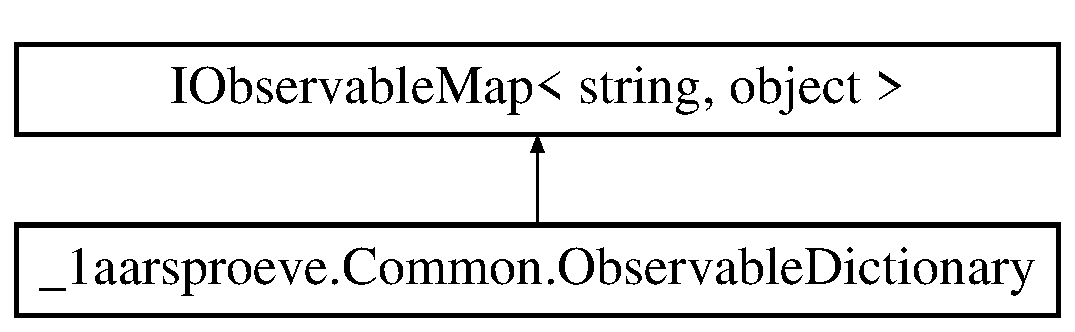
\includegraphics[height=2.000000cm]{class__1aarsproeve_1_1_common_1_1_observable_dictionary}
\end{center}
\end{figure}
\subsection*{Public Member Functions}
\begin{DoxyCompactItemize}
\item 
\hypertarget{class__1aarsproeve_1_1_common_1_1_observable_dictionary_a787ca1cf8774aa56af9dafe6e3200149}{}void {\bfseries Add} (string key, object value)\label{class__1aarsproeve_1_1_common_1_1_observable_dictionary_a787ca1cf8774aa56af9dafe6e3200149}

\item 
\hypertarget{class__1aarsproeve_1_1_common_1_1_observable_dictionary_a12559d5154e64bfa5b5fa2aac2785350}{}void {\bfseries Add} (Key\+Value\+Pair$<$ string, object $>$ item)\label{class__1aarsproeve_1_1_common_1_1_observable_dictionary_a12559d5154e64bfa5b5fa2aac2785350}

\item 
\hypertarget{class__1aarsproeve_1_1_common_1_1_observable_dictionary_a5be619bb4f70f093b6b6adf6f5782586}{}bool {\bfseries Remove} (string key)\label{class__1aarsproeve_1_1_common_1_1_observable_dictionary_a5be619bb4f70f093b6b6adf6f5782586}

\item 
\hypertarget{class__1aarsproeve_1_1_common_1_1_observable_dictionary_af32c84e07c21c32b99b406946c5908ab}{}bool {\bfseries Remove} (Key\+Value\+Pair$<$ string, object $>$ item)\label{class__1aarsproeve_1_1_common_1_1_observable_dictionary_af32c84e07c21c32b99b406946c5908ab}

\item 
\hypertarget{class__1aarsproeve_1_1_common_1_1_observable_dictionary_a2efbbb5591cdf7302dd208e2a92e9ab9}{}void {\bfseries Clear} ()\label{class__1aarsproeve_1_1_common_1_1_observable_dictionary_a2efbbb5591cdf7302dd208e2a92e9ab9}

\item 
\hypertarget{class__1aarsproeve_1_1_common_1_1_observable_dictionary_a91c13bcece087cdf96bf9eb68e261415}{}bool {\bfseries Contains\+Key} (string key)\label{class__1aarsproeve_1_1_common_1_1_observable_dictionary_a91c13bcece087cdf96bf9eb68e261415}

\item 
\hypertarget{class__1aarsproeve_1_1_common_1_1_observable_dictionary_acabb354db7da378b539a6c28d12b9e62}{}bool {\bfseries Try\+Get\+Value} (string key, out object value)\label{class__1aarsproeve_1_1_common_1_1_observable_dictionary_acabb354db7da378b539a6c28d12b9e62}

\item 
\hypertarget{class__1aarsproeve_1_1_common_1_1_observable_dictionary_a9963663b749dba524ef316b8672d64d6}{}bool {\bfseries Contains} (Key\+Value\+Pair$<$ string, object $>$ item)\label{class__1aarsproeve_1_1_common_1_1_observable_dictionary_a9963663b749dba524ef316b8672d64d6}

\item 
\hypertarget{class__1aarsproeve_1_1_common_1_1_observable_dictionary_abadc64539d7b13490598bcc56d022b73}{}I\+Enumerator$<$ Key\+Value\+Pair$<$ string, object $>$ $>$ {\bfseries Get\+Enumerator} ()\label{class__1aarsproeve_1_1_common_1_1_observable_dictionary_abadc64539d7b13490598bcc56d022b73}

\item 
\hypertarget{class__1aarsproeve_1_1_common_1_1_observable_dictionary_af9e531b5316ad474b4f25df585ab33a4}{}void {\bfseries Copy\+To} (Key\+Value\+Pair$<$ string, object $>$\mbox{[}$\,$\mbox{]} array, int array\+Index)\label{class__1aarsproeve_1_1_common_1_1_observable_dictionary_af9e531b5316ad474b4f25df585ab33a4}

\end{DoxyCompactItemize}
\subsection*{Properties}
\begin{DoxyCompactItemize}
\item 
\hypertarget{class__1aarsproeve_1_1_common_1_1_observable_dictionary_a56dda0334d80dd16118f7b8e14568e43}{}object {\bfseries this\mbox{[}string key\mbox{]}}\hspace{0.3cm}{\ttfamily  \mbox{[}get, set\mbox{]}}\label{class__1aarsproeve_1_1_common_1_1_observable_dictionary_a56dda0334d80dd16118f7b8e14568e43}

\item 
\hypertarget{class__1aarsproeve_1_1_common_1_1_observable_dictionary_a8a6b95aea01ec870543b13c234fddd26}{}I\+Collection$<$ string $>$ {\bfseries Keys}\hspace{0.3cm}{\ttfamily  \mbox{[}get\mbox{]}}\label{class__1aarsproeve_1_1_common_1_1_observable_dictionary_a8a6b95aea01ec870543b13c234fddd26}

\item 
\hypertarget{class__1aarsproeve_1_1_common_1_1_observable_dictionary_a3f266af47fb6ceaf4b3f3d65e2746229}{}I\+Collection$<$ object $>$ {\bfseries Values}\hspace{0.3cm}{\ttfamily  \mbox{[}get\mbox{]}}\label{class__1aarsproeve_1_1_common_1_1_observable_dictionary_a3f266af47fb6ceaf4b3f3d65e2746229}

\item 
\hypertarget{class__1aarsproeve_1_1_common_1_1_observable_dictionary_a5973a08feeb436962f7f0bdd571f0d65}{}int {\bfseries Count}\hspace{0.3cm}{\ttfamily  \mbox{[}get\mbox{]}}\label{class__1aarsproeve_1_1_common_1_1_observable_dictionary_a5973a08feeb436962f7f0bdd571f0d65}

\item 
\hypertarget{class__1aarsproeve_1_1_common_1_1_observable_dictionary_ade8478b862549e27c6862f8428593d6e}{}bool {\bfseries Is\+Read\+Only}\hspace{0.3cm}{\ttfamily  \mbox{[}get\mbox{]}}\label{class__1aarsproeve_1_1_common_1_1_observable_dictionary_ade8478b862549e27c6862f8428593d6e}

\end{DoxyCompactItemize}
\subsection*{Events}
\begin{DoxyCompactItemize}
\item 
\hypertarget{class__1aarsproeve_1_1_common_1_1_observable_dictionary_a313f6729d91091fa6c74f1bf58d195a1}{}Map\+Changed\+Event\+Handler$<$ string, object $>$ {\bfseries Map\+Changed}\label{class__1aarsproeve_1_1_common_1_1_observable_dictionary_a313f6729d91091fa6c74f1bf58d195a1}

\end{DoxyCompactItemize}


\subsection{Detailed Description}
Implementation of I\+Observable\+Map that supports reentrancy for use as a default view model. 



The documentation for this class was generated from the following file\+:\begin{DoxyCompactItemize}
\item 
C\+:/\+Users/\+Daniel\+Winther/\+Documents/\+Git\+Hub/1-\/aarsproeve/1aarsproeve/1aarsproeve/\+Common/Observable\+Dictionary.\+cs\end{DoxyCompactItemize}

\hypertarget{class__1aarsproeve_1_1_view_1_1_opret_bruger}{}\section{\+\_\+1aarsproeve.\+View.\+Opret\+Bruger Class Reference}
\label{class__1aarsproeve_1_1_view_1_1_opret_bruger}\index{\+\_\+1aarsproeve.\+View.\+Opret\+Bruger@{\+\_\+1aarsproeve.\+View.\+Opret\+Bruger}}


A basic page that provides characteristics common to most applications.  


Inheritance diagram for \+\_\+1aarsproeve.\+View.\+Opret\+Bruger\+:\begin{figure}[H]
\begin{center}
\leavevmode
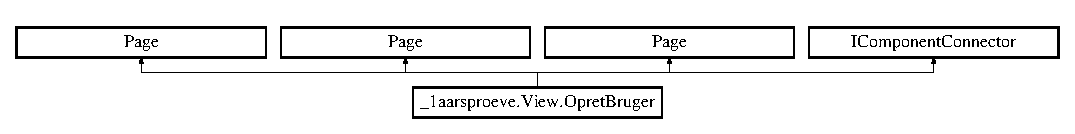
\includegraphics[height=1.359223cm]{class__1aarsproeve_1_1_view_1_1_opret_bruger}
\end{center}
\end{figure}
\subsection*{Public Member Functions}
\begin{DoxyCompactItemize}
\item 
\hypertarget{class__1aarsproeve_1_1_view_1_1_opret_bruger_a5e2f9fe203bec8aac1a9c705882502bd}{}void {\bfseries Connect} (int connection\+Id, object target)\label{class__1aarsproeve_1_1_view_1_1_opret_bruger_a5e2f9fe203bec8aac1a9c705882502bd}

\item 
\hypertarget{class__1aarsproeve_1_1_view_1_1_opret_bruger_a9d666a044c7981bc5099a366090dc726}{}void {\bfseries Initialize\+Component} ()\label{class__1aarsproeve_1_1_view_1_1_opret_bruger_a9d666a044c7981bc5099a366090dc726}

\end{DoxyCompactItemize}
\subsection*{Protected Member Functions}
\begin{DoxyCompactItemize}
\item 
override void \hyperlink{class__1aarsproeve_1_1_view_1_1_opret_bruger_a6c9f156568cc57390a59e547e497a65d}{On\+Navigated\+To} (Navigation\+Event\+Args e)
\item 
\hypertarget{class__1aarsproeve_1_1_view_1_1_opret_bruger_aba5e6a795635d072f688a7f378183b09}{}override void {\bfseries On\+Navigated\+From} (Navigation\+Event\+Args e)\label{class__1aarsproeve_1_1_view_1_1_opret_bruger_aba5e6a795635d072f688a7f378183b09}

\end{DoxyCompactItemize}
\subsection*{Properties}
\begin{DoxyCompactItemize}
\item 
\hyperlink{class__1aarsproeve_1_1_common_1_1_observable_dictionary}{Observable\+Dictionary} \hyperlink{class__1aarsproeve_1_1_view_1_1_opret_bruger_a597c247fbbf117d6d4ae8156433eb366}{Default\+View\+Model}\hspace{0.3cm}{\ttfamily  \mbox{[}get\mbox{]}}
\begin{DoxyCompactList}\small\item\em This can be changed to a strongly typed view model. \end{DoxyCompactList}\item 
\hyperlink{class__1aarsproeve_1_1_common_1_1_navigation_helper}{Navigation\+Helper} \hyperlink{class__1aarsproeve_1_1_view_1_1_opret_bruger_a3d67fd01a377d0a23130f57e9f785a46}{Navigation\+Helper}\hspace{0.3cm}{\ttfamily  \mbox{[}get\mbox{]}}
\begin{DoxyCompactList}\small\item\em Navigation\+Helper is used on each page to aid in navigation and process lifetime management \end{DoxyCompactList}\end{DoxyCompactItemize}


\subsection{Detailed Description}
A basic page that provides characteristics common to most applications. 



\subsection{Member Function Documentation}
\hypertarget{class__1aarsproeve_1_1_view_1_1_opret_bruger_a6c9f156568cc57390a59e547e497a65d}{}\index{\+\_\+1aarsproeve\+::\+View\+::\+Opret\+Bruger@{\+\_\+1aarsproeve\+::\+View\+::\+Opret\+Bruger}!On\+Navigated\+To@{On\+Navigated\+To}}
\index{On\+Navigated\+To@{On\+Navigated\+To}!\+\_\+1aarsproeve\+::\+View\+::\+Opret\+Bruger@{\+\_\+1aarsproeve\+::\+View\+::\+Opret\+Bruger}}
\subsubsection[{On\+Navigated\+To}]{\setlength{\rightskip}{0pt plus 5cm}override void \+\_\+1aarsproeve.\+View.\+Opret\+Bruger.\+On\+Navigated\+To (
\begin{DoxyParamCaption}
\item[{Navigation\+Event\+Args}]{e}
\end{DoxyParamCaption}
)\hspace{0.3cm}{\ttfamily [inline]}, {\ttfamily [protected]}}\label{class__1aarsproeve_1_1_view_1_1_opret_bruger_a6c9f156568cc57390a59e547e497a65d}
The methods provided in this section are simply used to allow Navigation\+Helper to respond to the page\textquotesingle{}s navigation methods.

Page specific logic should be placed in event handlers for the Grid\+C\+S.\+Common.\+Navigation\+Helper.\+Load\+State and Grid\+C\+S.\+Common.\+Navigation\+Helper.\+Save\+State. The navigation parameter is available in the Load\+State method in addition to page state preserved during an earlier session. 

\subsection{Property Documentation}
\hypertarget{class__1aarsproeve_1_1_view_1_1_opret_bruger_a597c247fbbf117d6d4ae8156433eb366}{}\index{\+\_\+1aarsproeve\+::\+View\+::\+Opret\+Bruger@{\+\_\+1aarsproeve\+::\+View\+::\+Opret\+Bruger}!Default\+View\+Model@{Default\+View\+Model}}
\index{Default\+View\+Model@{Default\+View\+Model}!\+\_\+1aarsproeve\+::\+View\+::\+Opret\+Bruger@{\+\_\+1aarsproeve\+::\+View\+::\+Opret\+Bruger}}
\subsubsection[{Default\+View\+Model}]{\setlength{\rightskip}{0pt plus 5cm}{\bf Observable\+Dictionary} \+\_\+1aarsproeve.\+View.\+Opret\+Bruger.\+Default\+View\+Model\hspace{0.3cm}{\ttfamily [get]}}\label{class__1aarsproeve_1_1_view_1_1_opret_bruger_a597c247fbbf117d6d4ae8156433eb366}


This can be changed to a strongly typed view model. 

\hypertarget{class__1aarsproeve_1_1_view_1_1_opret_bruger_a3d67fd01a377d0a23130f57e9f785a46}{}\index{\+\_\+1aarsproeve\+::\+View\+::\+Opret\+Bruger@{\+\_\+1aarsproeve\+::\+View\+::\+Opret\+Bruger}!Navigation\+Helper@{Navigation\+Helper}}
\index{Navigation\+Helper@{Navigation\+Helper}!\+\_\+1aarsproeve\+::\+View\+::\+Opret\+Bruger@{\+\_\+1aarsproeve\+::\+View\+::\+Opret\+Bruger}}
\subsubsection[{Navigation\+Helper}]{\setlength{\rightskip}{0pt plus 5cm}{\bf Navigation\+Helper} \+\_\+1aarsproeve.\+View.\+Opret\+Bruger.\+Navigation\+Helper\hspace{0.3cm}{\ttfamily [get]}}\label{class__1aarsproeve_1_1_view_1_1_opret_bruger_a3d67fd01a377d0a23130f57e9f785a46}


Navigation\+Helper is used on each page to aid in navigation and process lifetime management 



The documentation for this class was generated from the following files\+:\begin{DoxyCompactItemize}
\item 
Documents/\+Git\+Hub/1-\/aarsproeve/1aarsproeve/1aarsproeve/obj/\+Debug/\+View/Opret\+Bruger.\+g.\+cs\item 
Documents/\+Git\+Hub/1-\/aarsproeve/1aarsproeve/1aarsproeve/obj/\+Debug/\+View/Opret\+Bruger.\+g.\+i.\+cs\item 
Documents/\+Git\+Hub/1-\/aarsproeve/1aarsproeve/1aarsproeve/\+View/Opret\+Bruger.\+xaml.\+cs\end{DoxyCompactItemize}

\hypertarget{class__1aarsproeve_1_1_view_1_1_opret_vagt}{}\section{\+\_\+1aarsproeve.\+View.\+Opret\+Vagt Class Reference}
\label{class__1aarsproeve_1_1_view_1_1_opret_vagt}\index{\+\_\+1aarsproeve.\+View.\+Opret\+Vagt@{\+\_\+1aarsproeve.\+View.\+Opret\+Vagt}}


A basic page that provides characteristics common to most applications.  


Inheritance diagram for \+\_\+1aarsproeve.\+View.\+Opret\+Vagt\+:\begin{figure}[H]
\begin{center}
\leavevmode
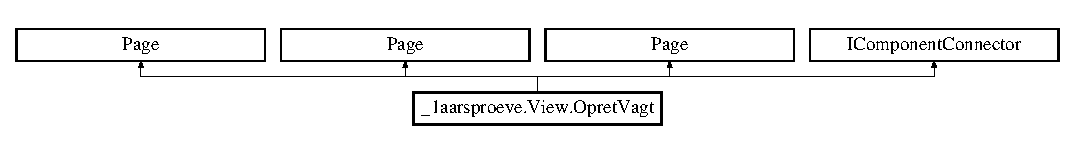
\includegraphics[height=1.450777cm]{class__1aarsproeve_1_1_view_1_1_opret_vagt}
\end{center}
\end{figure}
\subsection*{Public Member Functions}
\begin{DoxyCompactItemize}
\item 
\hypertarget{class__1aarsproeve_1_1_view_1_1_opret_vagt_a32f6f1d2b20a2a613647bf59c4fba582}{}void {\bfseries Connect} (int connection\+Id, object target)\label{class__1aarsproeve_1_1_view_1_1_opret_vagt_a32f6f1d2b20a2a613647bf59c4fba582}

\item 
\hypertarget{class__1aarsproeve_1_1_view_1_1_opret_vagt_a2c53ba2afdf89d829cf338652220e865}{}void {\bfseries Initialize\+Component} ()\label{class__1aarsproeve_1_1_view_1_1_opret_vagt_a2c53ba2afdf89d829cf338652220e865}

\end{DoxyCompactItemize}
\subsection*{Protected Member Functions}
\begin{DoxyCompactItemize}
\item 
override void \hyperlink{class__1aarsproeve_1_1_view_1_1_opret_vagt_a130f711b4eca04fe3eceb17b760f711b}{On\+Navigated\+To} (Navigation\+Event\+Args e)
\item 
\hypertarget{class__1aarsproeve_1_1_view_1_1_opret_vagt_a81ff62a8b1fdd64642bc7ed4354c0441}{}override void {\bfseries On\+Navigated\+From} (Navigation\+Event\+Args e)\label{class__1aarsproeve_1_1_view_1_1_opret_vagt_a81ff62a8b1fdd64642bc7ed4354c0441}

\end{DoxyCompactItemize}
\subsection*{Properties}
\begin{DoxyCompactItemize}
\item 
\hyperlink{class__1aarsproeve_1_1_common_1_1_observable_dictionary}{Observable\+Dictionary} \hyperlink{class__1aarsproeve_1_1_view_1_1_opret_vagt_a917197c5ec9ec6e45bfe1f8be3b5b544}{Default\+View\+Model}\hspace{0.3cm}{\ttfamily  \mbox{[}get\mbox{]}}
\begin{DoxyCompactList}\small\item\em This can be changed to a strongly typed view model. \end{DoxyCompactList}\item 
\hyperlink{class__1aarsproeve_1_1_common_1_1_navigation_helper}{Navigation\+Helper} \hyperlink{class__1aarsproeve_1_1_view_1_1_opret_vagt_ac175e006e267cf062167def039b8860c}{Navigation\+Helper}\hspace{0.3cm}{\ttfamily  \mbox{[}get\mbox{]}}
\begin{DoxyCompactList}\small\item\em Navigation\+Helper is used on each page to aid in navigation and process lifetime management \end{DoxyCompactList}\end{DoxyCompactItemize}


\subsection{Detailed Description}
A basic page that provides characteristics common to most applications. 



\subsection{Member Function Documentation}
\hypertarget{class__1aarsproeve_1_1_view_1_1_opret_vagt_a130f711b4eca04fe3eceb17b760f711b}{}\index{\+\_\+1aarsproeve\+::\+View\+::\+Opret\+Vagt@{\+\_\+1aarsproeve\+::\+View\+::\+Opret\+Vagt}!On\+Navigated\+To@{On\+Navigated\+To}}
\index{On\+Navigated\+To@{On\+Navigated\+To}!\+\_\+1aarsproeve\+::\+View\+::\+Opret\+Vagt@{\+\_\+1aarsproeve\+::\+View\+::\+Opret\+Vagt}}
\subsubsection[{On\+Navigated\+To}]{\setlength{\rightskip}{0pt plus 5cm}override void \+\_\+1aarsproeve.\+View.\+Opret\+Vagt.\+On\+Navigated\+To (
\begin{DoxyParamCaption}
\item[{Navigation\+Event\+Args}]{e}
\end{DoxyParamCaption}
)\hspace{0.3cm}{\ttfamily [inline]}, {\ttfamily [protected]}}\label{class__1aarsproeve_1_1_view_1_1_opret_vagt_a130f711b4eca04fe3eceb17b760f711b}
The methods provided in this section are simply used to allow Navigation\+Helper to respond to the page\textquotesingle{}s navigation methods.

Page specific logic should be placed in event handlers for the Grid\+C\+S.\+Common.\+Navigation\+Helper.\+Load\+State and Grid\+C\+S.\+Common.\+Navigation\+Helper.\+Save\+State. The navigation parameter is available in the Load\+State method in addition to page state preserved during an earlier session. 

\subsection{Property Documentation}
\hypertarget{class__1aarsproeve_1_1_view_1_1_opret_vagt_a917197c5ec9ec6e45bfe1f8be3b5b544}{}\index{\+\_\+1aarsproeve\+::\+View\+::\+Opret\+Vagt@{\+\_\+1aarsproeve\+::\+View\+::\+Opret\+Vagt}!Default\+View\+Model@{Default\+View\+Model}}
\index{Default\+View\+Model@{Default\+View\+Model}!\+\_\+1aarsproeve\+::\+View\+::\+Opret\+Vagt@{\+\_\+1aarsproeve\+::\+View\+::\+Opret\+Vagt}}
\subsubsection[{Default\+View\+Model}]{\setlength{\rightskip}{0pt plus 5cm}{\bf Observable\+Dictionary} \+\_\+1aarsproeve.\+View.\+Opret\+Vagt.\+Default\+View\+Model\hspace{0.3cm}{\ttfamily [get]}}\label{class__1aarsproeve_1_1_view_1_1_opret_vagt_a917197c5ec9ec6e45bfe1f8be3b5b544}


This can be changed to a strongly typed view model. 

\hypertarget{class__1aarsproeve_1_1_view_1_1_opret_vagt_ac175e006e267cf062167def039b8860c}{}\index{\+\_\+1aarsproeve\+::\+View\+::\+Opret\+Vagt@{\+\_\+1aarsproeve\+::\+View\+::\+Opret\+Vagt}!Navigation\+Helper@{Navigation\+Helper}}
\index{Navigation\+Helper@{Navigation\+Helper}!\+\_\+1aarsproeve\+::\+View\+::\+Opret\+Vagt@{\+\_\+1aarsproeve\+::\+View\+::\+Opret\+Vagt}}
\subsubsection[{Navigation\+Helper}]{\setlength{\rightskip}{0pt plus 5cm}{\bf Navigation\+Helper} \+\_\+1aarsproeve.\+View.\+Opret\+Vagt.\+Navigation\+Helper\hspace{0.3cm}{\ttfamily [get]}}\label{class__1aarsproeve_1_1_view_1_1_opret_vagt_ac175e006e267cf062167def039b8860c}


Navigation\+Helper is used on each page to aid in navigation and process lifetime management 



The documentation for this class was generated from the following files\+:\begin{DoxyCompactItemize}
\item 
C\+:/\+Users/\+Daniel\+Winther/\+Documents/\+Git\+Hub/1-\/aarsproeve/1aarsproeve/1aarsproeve/obj/\+Debug/\+View/Opret\+Vagt.\+g.\+cs\item 
C\+:/\+Users/\+Daniel\+Winther/\+Documents/\+Git\+Hub/1-\/aarsproeve/1aarsproeve/1aarsproeve/obj/\+Debug/\+View/Opret\+Vagt.\+g.\+i.\+cs\item 
C\+:/\+Users/\+Daniel\+Winther/\+Documents/\+Git\+Hub/1-\/aarsproeve/1aarsproeve/1aarsproeve/\+View/Opret\+Vagt.\+xaml.\+cs\end{DoxyCompactItemize}

\hypertarget{class__1aarsproeve_web_service_1_1_areas_1_1_help_page_1_1_model_descriptions_1_1_parameter_annotation}{}\section{\+\_\+1aarsproeve\+Web\+Service.\+Areas.\+Help\+Page.\+Model\+Descriptions.\+Parameter\+Annotation Class Reference}
\label{class__1aarsproeve_web_service_1_1_areas_1_1_help_page_1_1_model_descriptions_1_1_parameter_annotation}\index{\+\_\+1aarsproeve\+Web\+Service.\+Areas.\+Help\+Page.\+Model\+Descriptions.\+Parameter\+Annotation@{\+\_\+1aarsproeve\+Web\+Service.\+Areas.\+Help\+Page.\+Model\+Descriptions.\+Parameter\+Annotation}}
\subsection*{Properties}
\begin{DoxyCompactItemize}
\item 
\hypertarget{class__1aarsproeve_web_service_1_1_areas_1_1_help_page_1_1_model_descriptions_1_1_parameter_annotation_acd0669e175d07c79c1ec50f2bd9ddc0a}{}Attribute {\bfseries Annotation\+Attribute}\hspace{0.3cm}{\ttfamily  \mbox{[}get, set\mbox{]}}\label{class__1aarsproeve_web_service_1_1_areas_1_1_help_page_1_1_model_descriptions_1_1_parameter_annotation_acd0669e175d07c79c1ec50f2bd9ddc0a}

\item 
\hypertarget{class__1aarsproeve_web_service_1_1_areas_1_1_help_page_1_1_model_descriptions_1_1_parameter_annotation_a243d8f762b1bc6d9aa2bcef2b295f56d}{}string {\bfseries Documentation}\hspace{0.3cm}{\ttfamily  \mbox{[}get, set\mbox{]}}\label{class__1aarsproeve_web_service_1_1_areas_1_1_help_page_1_1_model_descriptions_1_1_parameter_annotation_a243d8f762b1bc6d9aa2bcef2b295f56d}

\end{DoxyCompactItemize}


The documentation for this class was generated from the following file\+:\begin{DoxyCompactItemize}
\item 
C\+:/\+Users/\+Daniel\+Winther/\+Documents/\+Git\+Hub/1-\/aarsproeve/1aarsproeve/1aarsproeve\+Web\+Service/\+Areas/\+Help\+Page/\+Model\+Descriptions/Parameter\+Annotation.\+cs\end{DoxyCompactItemize}

\hypertarget{class__1aarsproeve_web_service_1_1_areas_1_1_help_page_1_1_model_descriptions_1_1_parameter_description}{}\section{\+\_\+1aarsproeve\+Web\+Service.\+Areas.\+Help\+Page.\+Model\+Descriptions.\+Parameter\+Description Class Reference}
\label{class__1aarsproeve_web_service_1_1_areas_1_1_help_page_1_1_model_descriptions_1_1_parameter_description}\index{\+\_\+1aarsproeve\+Web\+Service.\+Areas.\+Help\+Page.\+Model\+Descriptions.\+Parameter\+Description@{\+\_\+1aarsproeve\+Web\+Service.\+Areas.\+Help\+Page.\+Model\+Descriptions.\+Parameter\+Description}}
\subsection*{Properties}
\begin{DoxyCompactItemize}
\item 
\hypertarget{class__1aarsproeve_web_service_1_1_areas_1_1_help_page_1_1_model_descriptions_1_1_parameter_description_a1b6f58c986d3889be141252c4ec520fc}{}Collection$<$ \hyperlink{class__1aarsproeve_web_service_1_1_areas_1_1_help_page_1_1_model_descriptions_1_1_parameter_annotation}{Parameter\+Annotation} $>$ {\bfseries Annotations}\hspace{0.3cm}{\ttfamily  \mbox{[}get\mbox{]}}\label{class__1aarsproeve_web_service_1_1_areas_1_1_help_page_1_1_model_descriptions_1_1_parameter_description_a1b6f58c986d3889be141252c4ec520fc}

\item 
\hypertarget{class__1aarsproeve_web_service_1_1_areas_1_1_help_page_1_1_model_descriptions_1_1_parameter_description_af387fc5f4d80c5592ef1635ed4232d3c}{}string {\bfseries Documentation}\hspace{0.3cm}{\ttfamily  \mbox{[}get, set\mbox{]}}\label{class__1aarsproeve_web_service_1_1_areas_1_1_help_page_1_1_model_descriptions_1_1_parameter_description_af387fc5f4d80c5592ef1635ed4232d3c}

\item 
\hypertarget{class__1aarsproeve_web_service_1_1_areas_1_1_help_page_1_1_model_descriptions_1_1_parameter_description_aa0ef3eefaa65192807631838a31f9b5d}{}string {\bfseries Name}\hspace{0.3cm}{\ttfamily  \mbox{[}get, set\mbox{]}}\label{class__1aarsproeve_web_service_1_1_areas_1_1_help_page_1_1_model_descriptions_1_1_parameter_description_aa0ef3eefaa65192807631838a31f9b5d}

\item 
\hypertarget{class__1aarsproeve_web_service_1_1_areas_1_1_help_page_1_1_model_descriptions_1_1_parameter_description_a0348d902ef3d41b4555e31c9a0421b6a}{}\hyperlink{class__1aarsproeve_web_service_1_1_areas_1_1_help_page_1_1_model_descriptions_1_1_model_description}{Model\+Description} {\bfseries Type\+Description}\hspace{0.3cm}{\ttfamily  \mbox{[}get, set\mbox{]}}\label{class__1aarsproeve_web_service_1_1_areas_1_1_help_page_1_1_model_descriptions_1_1_parameter_description_a0348d902ef3d41b4555e31c9a0421b6a}

\end{DoxyCompactItemize}


The documentation for this class was generated from the following file\+:\begin{DoxyCompactItemize}
\item 
C\+:/\+Users/\+Daniel\+Winther/\+Documents/\+Git\+Hub/1-\/aarsproeve/1aarsproeve/1aarsproeve\+Web\+Service/\+Areas/\+Help\+Page/\+Model\+Descriptions/Parameter\+Description.\+cs\end{DoxyCompactItemize}

\hypertarget{class__1aarsproeve_1_1_view_1_1_profil}{}\section{\+\_\+1aarsproeve.\+View.\+Profil Class Reference}
\label{class__1aarsproeve_1_1_view_1_1_profil}\index{\+\_\+1aarsproeve.\+View.\+Profil@{\+\_\+1aarsproeve.\+View.\+Profil}}


A basic page that provides characteristics common to most applications.  


Inheritance diagram for \+\_\+1aarsproeve.\+View.\+Profil\+:\begin{figure}[H]
\begin{center}
\leavevmode
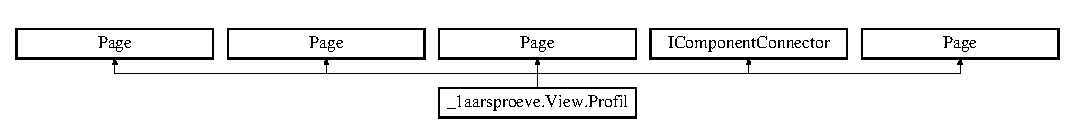
\includegraphics[height=1.357576cm]{class__1aarsproeve_1_1_view_1_1_profil}
\end{center}
\end{figure}
\subsection*{Public Member Functions}
\begin{DoxyCompactItemize}
\item 
\hypertarget{class__1aarsproeve_1_1_view_1_1_profil_a8a49f31d1274ad9f3d7dda340180166b}{}void {\bfseries Initialize\+Component} ()\label{class__1aarsproeve_1_1_view_1_1_profil_a8a49f31d1274ad9f3d7dda340180166b}

\item 
\hypertarget{class__1aarsproeve_1_1_view_1_1_profil_aef76942d2b54a5a91a00c1da9e18fed0}{}void {\bfseries Connect} (int connection\+Id, object target)\label{class__1aarsproeve_1_1_view_1_1_profil_aef76942d2b54a5a91a00c1da9e18fed0}

\item 
\hypertarget{class__1aarsproeve_1_1_view_1_1_profil_a8a49f31d1274ad9f3d7dda340180166b}{}void {\bfseries Initialize\+Component} ()\label{class__1aarsproeve_1_1_view_1_1_profil_a8a49f31d1274ad9f3d7dda340180166b}

\end{DoxyCompactItemize}
\subsection*{Protected Member Functions}
\begin{DoxyCompactItemize}
\item 
override void \hyperlink{class__1aarsproeve_1_1_view_1_1_profil_ab9fe2415e3f9fab8b95a4d10f374b8dd}{On\+Navigated\+To} (Navigation\+Event\+Args e)
\item 
\hypertarget{class__1aarsproeve_1_1_view_1_1_profil_a0104213a42510d9bad8143e22947a0b6}{}override void {\bfseries On\+Navigated\+From} (Navigation\+Event\+Args e)\label{class__1aarsproeve_1_1_view_1_1_profil_a0104213a42510d9bad8143e22947a0b6}

\end{DoxyCompactItemize}
\subsection*{Properties}
\begin{DoxyCompactItemize}
\item 
\hyperlink{class__1aarsproeve_1_1_common_1_1_observable_dictionary}{Observable\+Dictionary} \hyperlink{class__1aarsproeve_1_1_view_1_1_profil_ad66fb294e243d2475bc5d16da6ddfeb0}{Default\+View\+Model}\hspace{0.3cm}{\ttfamily  \mbox{[}get\mbox{]}}
\begin{DoxyCompactList}\small\item\em This can be changed to a strongly typed view model. \end{DoxyCompactList}\item 
\hyperlink{class__1aarsproeve_1_1_common_1_1_navigation_helper}{Navigation\+Helper} \hyperlink{class__1aarsproeve_1_1_view_1_1_profil_a16410b60470d2871c88c39af75b07130}{Navigation\+Helper}\hspace{0.3cm}{\ttfamily  \mbox{[}get\mbox{]}}
\begin{DoxyCompactList}\small\item\em Navigation\+Helper is used on each page to aid in navigation and process lifetime management \end{DoxyCompactList}\end{DoxyCompactItemize}


\subsection{Detailed Description}
A basic page that provides characteristics common to most applications. 



\subsection{Member Function Documentation}
\hypertarget{class__1aarsproeve_1_1_view_1_1_profil_ab9fe2415e3f9fab8b95a4d10f374b8dd}{}\index{\+\_\+1aarsproeve\+::\+View\+::\+Profil@{\+\_\+1aarsproeve\+::\+View\+::\+Profil}!On\+Navigated\+To@{On\+Navigated\+To}}
\index{On\+Navigated\+To@{On\+Navigated\+To}!\+\_\+1aarsproeve\+::\+View\+::\+Profil@{\+\_\+1aarsproeve\+::\+View\+::\+Profil}}
\subsubsection[{On\+Navigated\+To}]{\setlength{\rightskip}{0pt plus 5cm}override void \+\_\+1aarsproeve.\+View.\+Profil.\+On\+Navigated\+To (
\begin{DoxyParamCaption}
\item[{Navigation\+Event\+Args}]{e}
\end{DoxyParamCaption}
)\hspace{0.3cm}{\ttfamily [inline]}, {\ttfamily [protected]}}\label{class__1aarsproeve_1_1_view_1_1_profil_ab9fe2415e3f9fab8b95a4d10f374b8dd}
The methods provided in this section are simply used to allow Navigation\+Helper to respond to the page\textquotesingle{}s navigation methods.

Page specific logic should be placed in event handlers for the Grid\+C\+S.\+Common.\+Navigation\+Helper.\+Load\+State and Grid\+C\+S.\+Common.\+Navigation\+Helper.\+Save\+State. The navigation parameter is available in the Load\+State method in addition to page state preserved during an earlier session. 

\subsection{Property Documentation}
\hypertarget{class__1aarsproeve_1_1_view_1_1_profil_ad66fb294e243d2475bc5d16da6ddfeb0}{}\index{\+\_\+1aarsproeve\+::\+View\+::\+Profil@{\+\_\+1aarsproeve\+::\+View\+::\+Profil}!Default\+View\+Model@{Default\+View\+Model}}
\index{Default\+View\+Model@{Default\+View\+Model}!\+\_\+1aarsproeve\+::\+View\+::\+Profil@{\+\_\+1aarsproeve\+::\+View\+::\+Profil}}
\subsubsection[{Default\+View\+Model}]{\setlength{\rightskip}{0pt plus 5cm}{\bf Observable\+Dictionary} \+\_\+1aarsproeve.\+View.\+Profil.\+Default\+View\+Model\hspace{0.3cm}{\ttfamily [get]}}\label{class__1aarsproeve_1_1_view_1_1_profil_ad66fb294e243d2475bc5d16da6ddfeb0}


This can be changed to a strongly typed view model. 

\hypertarget{class__1aarsproeve_1_1_view_1_1_profil_a16410b60470d2871c88c39af75b07130}{}\index{\+\_\+1aarsproeve\+::\+View\+::\+Profil@{\+\_\+1aarsproeve\+::\+View\+::\+Profil}!Navigation\+Helper@{Navigation\+Helper}}
\index{Navigation\+Helper@{Navigation\+Helper}!\+\_\+1aarsproeve\+::\+View\+::\+Profil@{\+\_\+1aarsproeve\+::\+View\+::\+Profil}}
\subsubsection[{Navigation\+Helper}]{\setlength{\rightskip}{0pt plus 5cm}{\bf Navigation\+Helper} \+\_\+1aarsproeve.\+View.\+Profil.\+Navigation\+Helper\hspace{0.3cm}{\ttfamily [get]}}\label{class__1aarsproeve_1_1_view_1_1_profil_a16410b60470d2871c88c39af75b07130}


Navigation\+Helper is used on each page to aid in navigation and process lifetime management 



The documentation for this class was generated from the following files\+:\begin{DoxyCompactItemize}
\item 
C\+:/\+Users/\+Daniel\+Winther/\+Documents/\+Git\+Hub/1-\/aarsproeve/1aarsproeve/1aarsproeve/obj/\+Debug/\+View/Profil -\/ Copy.\+g.\+i.\+cs\item 
C\+:/\+Users/\+Daniel\+Winther/\+Documents/\+Git\+Hub/1-\/aarsproeve/1aarsproeve/1aarsproeve/obj/\+Debug/\+View/Profil.\+g.\+i.\+cs\item 
C\+:/\+Users/\+Daniel\+Winther/\+Documents/\+Git\+Hub/1-\/aarsproeve/1aarsproeve/1aarsproeve/\+View/Profil.\+xaml.\+cs\item 
C\+:/\+Users/\+Daniel\+Winther/\+Documents/\+Git\+Hub/1-\/aarsproeve/1aarsproeve/1aarsproeve/obj/\+Debug/\+View/Profil.\+g.\+cs\end{DoxyCompactItemize}

\hypertarget{class__1aarsproeve_1_1_view_1_1_rediger_vagt}{}\section{\+\_\+1aarsproeve.\+View.\+Rediger\+Vagt Class Reference}
\label{class__1aarsproeve_1_1_view_1_1_rediger_vagt}\index{\+\_\+1aarsproeve.\+View.\+Rediger\+Vagt@{\+\_\+1aarsproeve.\+View.\+Rediger\+Vagt}}


A basic page that provides characteristics common to most applications.  


Inheritance diagram for \+\_\+1aarsproeve.\+View.\+Rediger\+Vagt\+:\begin{figure}[H]
\begin{center}
\leavevmode
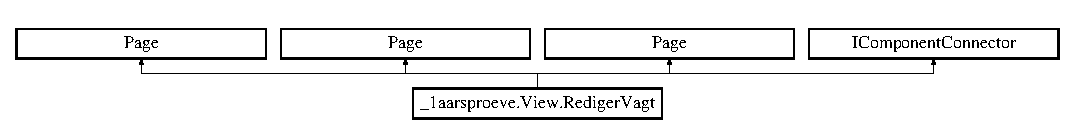
\includegraphics[height=1.365854cm]{class__1aarsproeve_1_1_view_1_1_rediger_vagt}
\end{center}
\end{figure}
\subsection*{Public Member Functions}
\begin{DoxyCompactItemize}
\item 
\hypertarget{class__1aarsproeve_1_1_view_1_1_rediger_vagt_aadd8614ddc572e62fe046f7fa5a3897a}{}void {\bfseries Connect} (int connection\+Id, object target)\label{class__1aarsproeve_1_1_view_1_1_rediger_vagt_aadd8614ddc572e62fe046f7fa5a3897a}

\item 
\hypertarget{class__1aarsproeve_1_1_view_1_1_rediger_vagt_aa6fd55b8255bfb967ce2eb82b6f4c68d}{}void {\bfseries Initialize\+Component} ()\label{class__1aarsproeve_1_1_view_1_1_rediger_vagt_aa6fd55b8255bfb967ce2eb82b6f4c68d}

\end{DoxyCompactItemize}
\subsection*{Protected Member Functions}
\begin{DoxyCompactItemize}
\item 
override void \hyperlink{class__1aarsproeve_1_1_view_1_1_rediger_vagt_adccbdc0bca2c6ca8429f8510816a0701}{On\+Navigated\+To} (Navigation\+Event\+Args e)
\item 
\hypertarget{class__1aarsproeve_1_1_view_1_1_rediger_vagt_a1d27c2a52dfaca570b513aba86b023a2}{}override void {\bfseries On\+Navigated\+From} (Navigation\+Event\+Args e)\label{class__1aarsproeve_1_1_view_1_1_rediger_vagt_a1d27c2a52dfaca570b513aba86b023a2}

\end{DoxyCompactItemize}
\subsection*{Properties}
\begin{DoxyCompactItemize}
\item 
\hyperlink{class__1aarsproeve_1_1_common_1_1_observable_dictionary}{Observable\+Dictionary} \hyperlink{class__1aarsproeve_1_1_view_1_1_rediger_vagt_af2df54817af67729bd484de917de7bb2}{Default\+View\+Model}\hspace{0.3cm}{\ttfamily  \mbox{[}get\mbox{]}}
\begin{DoxyCompactList}\small\item\em This can be changed to a strongly typed view model. \end{DoxyCompactList}\item 
\hyperlink{class__1aarsproeve_1_1_common_1_1_navigation_helper}{Navigation\+Helper} \hyperlink{class__1aarsproeve_1_1_view_1_1_rediger_vagt_a205f8abe3b935baab61ee977737d2e03}{Navigation\+Helper}\hspace{0.3cm}{\ttfamily  \mbox{[}get\mbox{]}}
\begin{DoxyCompactList}\small\item\em Navigation\+Helper is used on each page to aid in navigation and process lifetime management \end{DoxyCompactList}\end{DoxyCompactItemize}


\subsection{Detailed Description}
A basic page that provides characteristics common to most applications. 



\subsection{Member Function Documentation}
\hypertarget{class__1aarsproeve_1_1_view_1_1_rediger_vagt_adccbdc0bca2c6ca8429f8510816a0701}{}\index{\+\_\+1aarsproeve\+::\+View\+::\+Rediger\+Vagt@{\+\_\+1aarsproeve\+::\+View\+::\+Rediger\+Vagt}!On\+Navigated\+To@{On\+Navigated\+To}}
\index{On\+Navigated\+To@{On\+Navigated\+To}!\+\_\+1aarsproeve\+::\+View\+::\+Rediger\+Vagt@{\+\_\+1aarsproeve\+::\+View\+::\+Rediger\+Vagt}}
\subsubsection[{On\+Navigated\+To}]{\setlength{\rightskip}{0pt plus 5cm}override void \+\_\+1aarsproeve.\+View.\+Rediger\+Vagt.\+On\+Navigated\+To (
\begin{DoxyParamCaption}
\item[{Navigation\+Event\+Args}]{e}
\end{DoxyParamCaption}
)\hspace{0.3cm}{\ttfamily [inline]}, {\ttfamily [protected]}}\label{class__1aarsproeve_1_1_view_1_1_rediger_vagt_adccbdc0bca2c6ca8429f8510816a0701}
The methods provided in this section are simply used to allow Navigation\+Helper to respond to the page\textquotesingle{}s navigation methods.

Page specific logic should be placed in event handlers for the Grid\+C\+S.\+Common.\+Navigation\+Helper.\+Load\+State and Grid\+C\+S.\+Common.\+Navigation\+Helper.\+Save\+State. The navigation parameter is available in the Load\+State method in addition to page state preserved during an earlier session. 

\subsection{Property Documentation}
\hypertarget{class__1aarsproeve_1_1_view_1_1_rediger_vagt_af2df54817af67729bd484de917de7bb2}{}\index{\+\_\+1aarsproeve\+::\+View\+::\+Rediger\+Vagt@{\+\_\+1aarsproeve\+::\+View\+::\+Rediger\+Vagt}!Default\+View\+Model@{Default\+View\+Model}}
\index{Default\+View\+Model@{Default\+View\+Model}!\+\_\+1aarsproeve\+::\+View\+::\+Rediger\+Vagt@{\+\_\+1aarsproeve\+::\+View\+::\+Rediger\+Vagt}}
\subsubsection[{Default\+View\+Model}]{\setlength{\rightskip}{0pt plus 5cm}{\bf Observable\+Dictionary} \+\_\+1aarsproeve.\+View.\+Rediger\+Vagt.\+Default\+View\+Model\hspace{0.3cm}{\ttfamily [get]}}\label{class__1aarsproeve_1_1_view_1_1_rediger_vagt_af2df54817af67729bd484de917de7bb2}


This can be changed to a strongly typed view model. 

\hypertarget{class__1aarsproeve_1_1_view_1_1_rediger_vagt_a205f8abe3b935baab61ee977737d2e03}{}\index{\+\_\+1aarsproeve\+::\+View\+::\+Rediger\+Vagt@{\+\_\+1aarsproeve\+::\+View\+::\+Rediger\+Vagt}!Navigation\+Helper@{Navigation\+Helper}}
\index{Navigation\+Helper@{Navigation\+Helper}!\+\_\+1aarsproeve\+::\+View\+::\+Rediger\+Vagt@{\+\_\+1aarsproeve\+::\+View\+::\+Rediger\+Vagt}}
\subsubsection[{Navigation\+Helper}]{\setlength{\rightskip}{0pt plus 5cm}{\bf Navigation\+Helper} \+\_\+1aarsproeve.\+View.\+Rediger\+Vagt.\+Navigation\+Helper\hspace{0.3cm}{\ttfamily [get]}}\label{class__1aarsproeve_1_1_view_1_1_rediger_vagt_a205f8abe3b935baab61ee977737d2e03}


Navigation\+Helper is used on each page to aid in navigation and process lifetime management 



The documentation for this class was generated from the following files\+:\begin{DoxyCompactItemize}
\item 
Documents/\+Git\+Hub/1-\/aarsproeve/1aarsproeve/1aarsproeve/obj/\+Debug/\+View/Rediger\+Vagt.\+g.\+cs\item 
Documents/\+Git\+Hub/1-\/aarsproeve/1aarsproeve/1aarsproeve/obj/\+Debug/\+View/Rediger\+Vagt.\+g.\+i.\+cs\item 
Documents/\+Git\+Hub/1-\/aarsproeve/1aarsproeve/1aarsproeve/\+View/Rediger\+Vagt.\+xaml.\+cs\end{DoxyCompactItemize}

\hypertarget{class__1aarsproeve_1_1_common_1_1_relay_command}{}\section{\+\_\+1aarsproeve.\+Common.\+Relay\+Command Class Reference}
\label{class__1aarsproeve_1_1_common_1_1_relay_command}\index{\+\_\+1aarsproeve.\+Common.\+Relay\+Command@{\+\_\+1aarsproeve.\+Common.\+Relay\+Command}}


A command whose sole purpose is to relay its functionality to other objects by invoking delegates. The default return value for the Can\+Execute method is \textquotesingle{}true\textquotesingle{}. \hyperlink{class__1aarsproeve_1_1_common_1_1_relay_command_a90744bca5c47a6c212fd7d0cb89182f1}{Raise\+Can\+Execute\+Changed} needs to be called whenever \hyperlink{class__1aarsproeve_1_1_common_1_1_relay_command_a3c52d00e1d9ab7ab06cc4244b50fbee2}{Can\+Execute} is expected to return a different value.  


Inheritance diagram for \+\_\+1aarsproeve.\+Common.\+Relay\+Command\+:\begin{figure}[H]
\begin{center}
\leavevmode
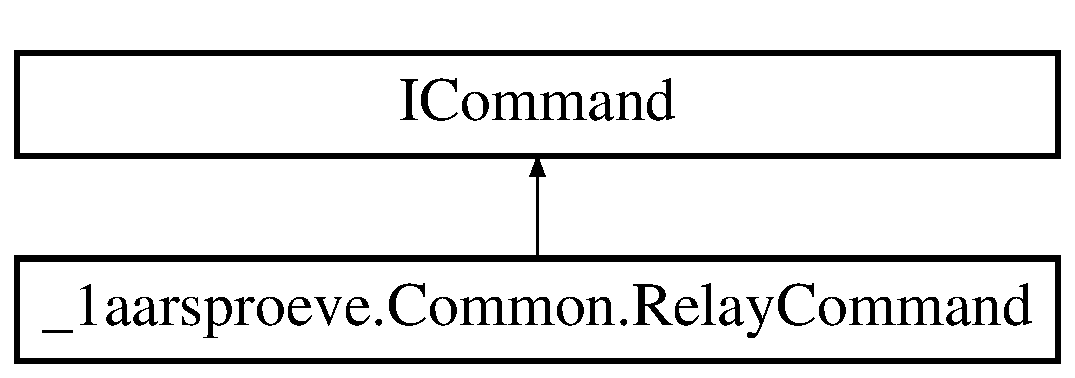
\includegraphics[height=2.000000cm]{class__1aarsproeve_1_1_common_1_1_relay_command}
\end{center}
\end{figure}
\subsection*{Public Member Functions}
\begin{DoxyCompactItemize}
\item 
\hyperlink{class__1aarsproeve_1_1_common_1_1_relay_command_ab592bbed4e6cfd1559dcaffe23223a13}{Relay\+Command} (Action execute)
\begin{DoxyCompactList}\small\item\em Creates a new command that can always execute. \end{DoxyCompactList}\item 
\hyperlink{class__1aarsproeve_1_1_common_1_1_relay_command_a29a92428317c491efba524c871cce065}{Relay\+Command} (Action execute, Func$<$ bool $>$ can\+Execute)
\begin{DoxyCompactList}\small\item\em Creates a new command. \end{DoxyCompactList}\item 
bool \hyperlink{class__1aarsproeve_1_1_common_1_1_relay_command_a3c52d00e1d9ab7ab06cc4244b50fbee2}{Can\+Execute} (object parameter)
\begin{DoxyCompactList}\small\item\em Determines whether this \hyperlink{class__1aarsproeve_1_1_common_1_1_relay_command}{Relay\+Command} can execute in its current state. \end{DoxyCompactList}\item 
void \hyperlink{class__1aarsproeve_1_1_common_1_1_relay_command_a0958a03842d5de3567d9e644026046b3}{Execute} (object parameter)
\begin{DoxyCompactList}\small\item\em Executes the \hyperlink{class__1aarsproeve_1_1_common_1_1_relay_command}{Relay\+Command} on the current command target. \end{DoxyCompactList}\item 
void \hyperlink{class__1aarsproeve_1_1_common_1_1_relay_command_a90744bca5c47a6c212fd7d0cb89182f1}{Raise\+Can\+Execute\+Changed} ()
\begin{DoxyCompactList}\small\item\em Method used to raise the \hyperlink{class__1aarsproeve_1_1_common_1_1_relay_command_a4502fa3e74d23cc9cd33cec559e96390}{Can\+Execute\+Changed} event to indicate that the return value of the \hyperlink{class__1aarsproeve_1_1_common_1_1_relay_command_a3c52d00e1d9ab7ab06cc4244b50fbee2}{Can\+Execute} method has changed. \end{DoxyCompactList}\end{DoxyCompactItemize}
\subsection*{Events}
\begin{DoxyCompactItemize}
\item 
Event\+Handler \hyperlink{class__1aarsproeve_1_1_common_1_1_relay_command_a4502fa3e74d23cc9cd33cec559e96390}{Can\+Execute\+Changed}
\begin{DoxyCompactList}\small\item\em Raised when Raise\+Can\+Execute\+Changed is called. \end{DoxyCompactList}\end{DoxyCompactItemize}


\subsection{Detailed Description}
A command whose sole purpose is to relay its functionality to other objects by invoking delegates. The default return value for the Can\+Execute method is \textquotesingle{}true\textquotesingle{}. \hyperlink{class__1aarsproeve_1_1_common_1_1_relay_command_a90744bca5c47a6c212fd7d0cb89182f1}{Raise\+Can\+Execute\+Changed} needs to be called whenever \hyperlink{class__1aarsproeve_1_1_common_1_1_relay_command_a3c52d00e1d9ab7ab06cc4244b50fbee2}{Can\+Execute} is expected to return a different value. 



\subsection{Constructor \& Destructor Documentation}
\hypertarget{class__1aarsproeve_1_1_common_1_1_relay_command_ab592bbed4e6cfd1559dcaffe23223a13}{}\index{\+\_\+1aarsproeve\+::\+Common\+::\+Relay\+Command@{\+\_\+1aarsproeve\+::\+Common\+::\+Relay\+Command}!Relay\+Command@{Relay\+Command}}
\index{Relay\+Command@{Relay\+Command}!\+\_\+1aarsproeve\+::\+Common\+::\+Relay\+Command@{\+\_\+1aarsproeve\+::\+Common\+::\+Relay\+Command}}
\subsubsection[{Relay\+Command}]{\setlength{\rightskip}{0pt plus 5cm}\+\_\+1aarsproeve.\+Common.\+Relay\+Command.\+Relay\+Command (
\begin{DoxyParamCaption}
\item[{Action}]{execute}
\end{DoxyParamCaption}
)}\label{class__1aarsproeve_1_1_common_1_1_relay_command_ab592bbed4e6cfd1559dcaffe23223a13}


Creates a new command that can always execute. 


\begin{DoxyParams}{Parameters}
{\em execute} & The execution logic.\\
\hline
\end{DoxyParams}
\hypertarget{class__1aarsproeve_1_1_common_1_1_relay_command_a29a92428317c491efba524c871cce065}{}\index{\+\_\+1aarsproeve\+::\+Common\+::\+Relay\+Command@{\+\_\+1aarsproeve\+::\+Common\+::\+Relay\+Command}!Relay\+Command@{Relay\+Command}}
\index{Relay\+Command@{Relay\+Command}!\+\_\+1aarsproeve\+::\+Common\+::\+Relay\+Command@{\+\_\+1aarsproeve\+::\+Common\+::\+Relay\+Command}}
\subsubsection[{Relay\+Command}]{\setlength{\rightskip}{0pt plus 5cm}\+\_\+1aarsproeve.\+Common.\+Relay\+Command.\+Relay\+Command (
\begin{DoxyParamCaption}
\item[{Action}]{execute, }
\item[{Func$<$ bool $>$}]{can\+Execute}
\end{DoxyParamCaption}
)}\label{class__1aarsproeve_1_1_common_1_1_relay_command_a29a92428317c491efba524c871cce065}


Creates a new command. 


\begin{DoxyParams}{Parameters}
{\em execute} & The execution logic.\\
\hline
{\em can\+Execute} & The execution status logic.\\
\hline
\end{DoxyParams}


\subsection{Member Function Documentation}
\hypertarget{class__1aarsproeve_1_1_common_1_1_relay_command_a3c52d00e1d9ab7ab06cc4244b50fbee2}{}\index{\+\_\+1aarsproeve\+::\+Common\+::\+Relay\+Command@{\+\_\+1aarsproeve\+::\+Common\+::\+Relay\+Command}!Can\+Execute@{Can\+Execute}}
\index{Can\+Execute@{Can\+Execute}!\+\_\+1aarsproeve\+::\+Common\+::\+Relay\+Command@{\+\_\+1aarsproeve\+::\+Common\+::\+Relay\+Command}}
\subsubsection[{Can\+Execute}]{\setlength{\rightskip}{0pt plus 5cm}bool \+\_\+1aarsproeve.\+Common.\+Relay\+Command.\+Can\+Execute (
\begin{DoxyParamCaption}
\item[{object}]{parameter}
\end{DoxyParamCaption}
)}\label{class__1aarsproeve_1_1_common_1_1_relay_command_a3c52d00e1d9ab7ab06cc4244b50fbee2}


Determines whether this \hyperlink{class__1aarsproeve_1_1_common_1_1_relay_command}{Relay\+Command} can execute in its current state. 


\begin{DoxyParams}{Parameters}
{\em parameter} & Data used by the command. If the command does not require data to be passed, this object can be set to null. \\
\hline
\end{DoxyParams}
\begin{DoxyReturn}{Returns}
true if this command can be executed; otherwise, false.
\end{DoxyReturn}
\hypertarget{class__1aarsproeve_1_1_common_1_1_relay_command_a0958a03842d5de3567d9e644026046b3}{}\index{\+\_\+1aarsproeve\+::\+Common\+::\+Relay\+Command@{\+\_\+1aarsproeve\+::\+Common\+::\+Relay\+Command}!Execute@{Execute}}
\index{Execute@{Execute}!\+\_\+1aarsproeve\+::\+Common\+::\+Relay\+Command@{\+\_\+1aarsproeve\+::\+Common\+::\+Relay\+Command}}
\subsubsection[{Execute}]{\setlength{\rightskip}{0pt plus 5cm}void \+\_\+1aarsproeve.\+Common.\+Relay\+Command.\+Execute (
\begin{DoxyParamCaption}
\item[{object}]{parameter}
\end{DoxyParamCaption}
)}\label{class__1aarsproeve_1_1_common_1_1_relay_command_a0958a03842d5de3567d9e644026046b3}


Executes the \hyperlink{class__1aarsproeve_1_1_common_1_1_relay_command}{Relay\+Command} on the current command target. 


\begin{DoxyParams}{Parameters}
{\em parameter} & Data used by the command. If the command does not require data to be passed, this object can be set to null. \\
\hline
\end{DoxyParams}
\hypertarget{class__1aarsproeve_1_1_common_1_1_relay_command_a90744bca5c47a6c212fd7d0cb89182f1}{}\index{\+\_\+1aarsproeve\+::\+Common\+::\+Relay\+Command@{\+\_\+1aarsproeve\+::\+Common\+::\+Relay\+Command}!Raise\+Can\+Execute\+Changed@{Raise\+Can\+Execute\+Changed}}
\index{Raise\+Can\+Execute\+Changed@{Raise\+Can\+Execute\+Changed}!\+\_\+1aarsproeve\+::\+Common\+::\+Relay\+Command@{\+\_\+1aarsproeve\+::\+Common\+::\+Relay\+Command}}
\subsubsection[{Raise\+Can\+Execute\+Changed}]{\setlength{\rightskip}{0pt plus 5cm}void \+\_\+1aarsproeve.\+Common.\+Relay\+Command.\+Raise\+Can\+Execute\+Changed (
\begin{DoxyParamCaption}
{}
\end{DoxyParamCaption}
)}\label{class__1aarsproeve_1_1_common_1_1_relay_command_a90744bca5c47a6c212fd7d0cb89182f1}


Method used to raise the \hyperlink{class__1aarsproeve_1_1_common_1_1_relay_command_a4502fa3e74d23cc9cd33cec559e96390}{Can\+Execute\+Changed} event to indicate that the return value of the \hyperlink{class__1aarsproeve_1_1_common_1_1_relay_command_a3c52d00e1d9ab7ab06cc4244b50fbee2}{Can\+Execute} method has changed. 



\subsection{Event Documentation}
\hypertarget{class__1aarsproeve_1_1_common_1_1_relay_command_a4502fa3e74d23cc9cd33cec559e96390}{}\index{\+\_\+1aarsproeve\+::\+Common\+::\+Relay\+Command@{\+\_\+1aarsproeve\+::\+Common\+::\+Relay\+Command}!Can\+Execute\+Changed@{Can\+Execute\+Changed}}
\index{Can\+Execute\+Changed@{Can\+Execute\+Changed}!\+\_\+1aarsproeve\+::\+Common\+::\+Relay\+Command@{\+\_\+1aarsproeve\+::\+Common\+::\+Relay\+Command}}
\subsubsection[{Can\+Execute\+Changed}]{\setlength{\rightskip}{0pt plus 5cm}Event\+Handler \+\_\+1aarsproeve.\+Common.\+Relay\+Command.\+Can\+Execute\+Changed}\label{class__1aarsproeve_1_1_common_1_1_relay_command_a4502fa3e74d23cc9cd33cec559e96390}


Raised when Raise\+Can\+Execute\+Changed is called. 



The documentation for this class was generated from the following file\+:\begin{DoxyCompactItemize}
\item 
Documents/\+Git\+Hub/1-\/aarsproeve/1aarsproeve/1aarsproeve/\+Common/Relay\+Command.\+cs\end{DoxyCompactItemize}

\hypertarget{class__1aarsproeve_web_service_1_1_route_config}{}\section{\+\_\+1aarsproeve\+Web\+Service.\+Route\+Config Class Reference}
\label{class__1aarsproeve_web_service_1_1_route_config}\index{\+\_\+1aarsproeve\+Web\+Service.\+Route\+Config@{\+\_\+1aarsproeve\+Web\+Service.\+Route\+Config}}
\subsection*{Static Public Member Functions}
\begin{DoxyCompactItemize}
\item 
\hypertarget{class__1aarsproeve_web_service_1_1_route_config_a2e7e1e761cec2f6d6ff22df4340a30d0}{}static void {\bfseries Register\+Routes} (Route\+Collection routes)\label{class__1aarsproeve_web_service_1_1_route_config_a2e7e1e761cec2f6d6ff22df4340a30d0}

\end{DoxyCompactItemize}


The documentation for this class was generated from the following file\+:\begin{DoxyCompactItemize}
\item 
C\+:/\+Users/\+Daniel\+Winther/\+Documents/\+Git\+Hub/1-\/aarsproeve/1aarsproeve/1aarsproeve\+Web\+Service/\+App\+\_\+\+Start/Route\+Config.\+cs\end{DoxyCompactItemize}

\hypertarget{class__1aarsproeve_1_1_common_1_1_save_state_event_args}{}\section{\+\_\+1aarsproeve.\+Common.\+Save\+State\+Event\+Args Class Reference}
\label{class__1aarsproeve_1_1_common_1_1_save_state_event_args}\index{\+\_\+1aarsproeve.\+Common.\+Save\+State\+Event\+Args@{\+\_\+1aarsproeve.\+Common.\+Save\+State\+Event\+Args}}


Class used to hold the event data required when a page attempts to save state.  


Inheritance diagram for \+\_\+1aarsproeve.\+Common.\+Save\+State\+Event\+Args\+:\begin{figure}[H]
\begin{center}
\leavevmode
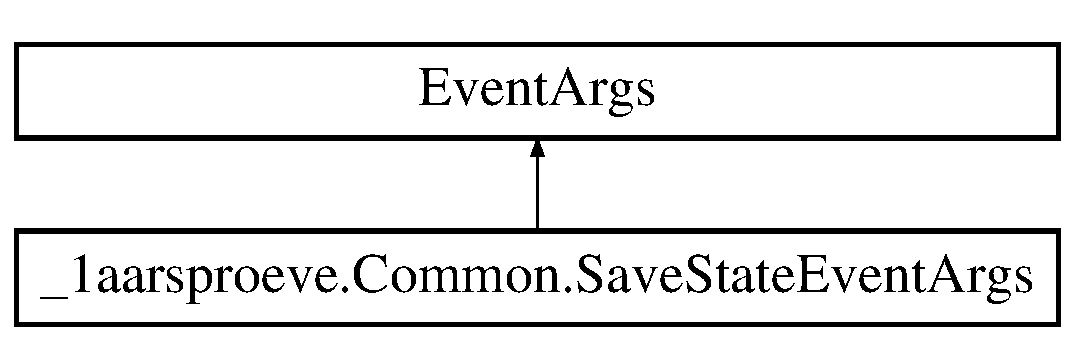
\includegraphics[height=2.000000cm]{class__1aarsproeve_1_1_common_1_1_save_state_event_args}
\end{center}
\end{figure}
\subsection*{Public Member Functions}
\begin{DoxyCompactItemize}
\item 
\hyperlink{class__1aarsproeve_1_1_common_1_1_save_state_event_args_ada2f56029afefc9938cb8567190037f9}{Save\+State\+Event\+Args} (Dictionary$<$ string, Object $>$ page\+State)
\begin{DoxyCompactList}\small\item\em Initializes a new instance of the \hyperlink{class__1aarsproeve_1_1_common_1_1_save_state_event_args}{Save\+State\+Event\+Args} class. \end{DoxyCompactList}\end{DoxyCompactItemize}
\subsection*{Properties}
\begin{DoxyCompactItemize}
\item 
Dictionary$<$ string, Object $>$ \hyperlink{class__1aarsproeve_1_1_common_1_1_save_state_event_args_a8c2a073606d2429d985a1747707c6c29}{Page\+State}\hspace{0.3cm}{\ttfamily  \mbox{[}get\mbox{]}}
\begin{DoxyCompactList}\small\item\em An empty dictionary to be populated with serializable state. \end{DoxyCompactList}\end{DoxyCompactItemize}


\subsection{Detailed Description}
Class used to hold the event data required when a page attempts to save state. 



\subsection{Constructor \& Destructor Documentation}
\hypertarget{class__1aarsproeve_1_1_common_1_1_save_state_event_args_ada2f56029afefc9938cb8567190037f9}{}\index{\+\_\+1aarsproeve\+::\+Common\+::\+Save\+State\+Event\+Args@{\+\_\+1aarsproeve\+::\+Common\+::\+Save\+State\+Event\+Args}!Save\+State\+Event\+Args@{Save\+State\+Event\+Args}}
\index{Save\+State\+Event\+Args@{Save\+State\+Event\+Args}!\+\_\+1aarsproeve\+::\+Common\+::\+Save\+State\+Event\+Args@{\+\_\+1aarsproeve\+::\+Common\+::\+Save\+State\+Event\+Args}}
\subsubsection[{Save\+State\+Event\+Args}]{\setlength{\rightskip}{0pt plus 5cm}\+\_\+1aarsproeve.\+Common.\+Save\+State\+Event\+Args.\+Save\+State\+Event\+Args (
\begin{DoxyParamCaption}
\item[{Dictionary$<$ string, Object $>$}]{page\+State}
\end{DoxyParamCaption}
)\hspace{0.3cm}{\ttfamily [inline]}}\label{class__1aarsproeve_1_1_common_1_1_save_state_event_args_ada2f56029afefc9938cb8567190037f9}


Initializes a new instance of the \hyperlink{class__1aarsproeve_1_1_common_1_1_save_state_event_args}{Save\+State\+Event\+Args} class. 


\begin{DoxyParams}{Parameters}
{\em page\+State} & An empty dictionary to be populated with serializable state.\\
\hline
\end{DoxyParams}


\subsection{Property Documentation}
\hypertarget{class__1aarsproeve_1_1_common_1_1_save_state_event_args_a8c2a073606d2429d985a1747707c6c29}{}\index{\+\_\+1aarsproeve\+::\+Common\+::\+Save\+State\+Event\+Args@{\+\_\+1aarsproeve\+::\+Common\+::\+Save\+State\+Event\+Args}!Page\+State@{Page\+State}}
\index{Page\+State@{Page\+State}!\+\_\+1aarsproeve\+::\+Common\+::\+Save\+State\+Event\+Args@{\+\_\+1aarsproeve\+::\+Common\+::\+Save\+State\+Event\+Args}}
\subsubsection[{Page\+State}]{\setlength{\rightskip}{0pt plus 5cm}Dictionary$<$string, Object$>$ \+\_\+1aarsproeve.\+Common.\+Save\+State\+Event\+Args.\+Page\+State\hspace{0.3cm}{\ttfamily [get]}}\label{class__1aarsproeve_1_1_common_1_1_save_state_event_args_a8c2a073606d2429d985a1747707c6c29}


An empty dictionary to be populated with serializable state. 



The documentation for this class was generated from the following file\+:\begin{DoxyCompactItemize}
\item 
Documents/\+Git\+Hub/1-\/aarsproeve/1aarsproeve/1aarsproeve/\+Common/Navigation\+Helper.\+cs\end{DoxyCompactItemize}

\hypertarget{class__1aarsproeve_web_service_1_1_areas_1_1_help_page_1_1_model_descriptions_1_1_simple_type_model_description}{}\section{\+\_\+1aarsproeve\+Web\+Service.\+Areas.\+Help\+Page.\+Model\+Descriptions.\+Simple\+Type\+Model\+Description Class Reference}
\label{class__1aarsproeve_web_service_1_1_areas_1_1_help_page_1_1_model_descriptions_1_1_simple_type_model_description}\index{\+\_\+1aarsproeve\+Web\+Service.\+Areas.\+Help\+Page.\+Model\+Descriptions.\+Simple\+Type\+Model\+Description@{\+\_\+1aarsproeve\+Web\+Service.\+Areas.\+Help\+Page.\+Model\+Descriptions.\+Simple\+Type\+Model\+Description}}
Inheritance diagram for \+\_\+1aarsproeve\+Web\+Service.\+Areas.\+Help\+Page.\+Model\+Descriptions.\+Simple\+Type\+Model\+Description\+:\begin{figure}[H]
\begin{center}
\leavevmode
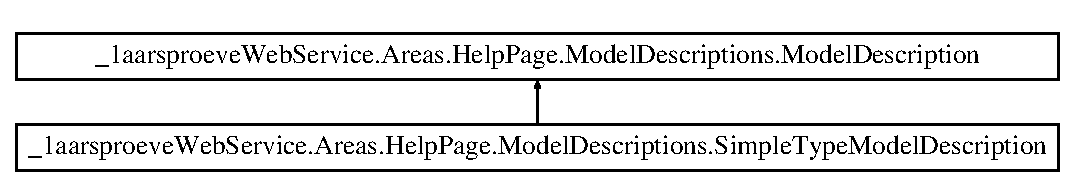
\includegraphics[height=2.000000cm]{class__1aarsproeve_web_service_1_1_areas_1_1_help_page_1_1_model_descriptions_1_1_simple_type_model_description}
\end{center}
\end{figure}
\subsection*{Additional Inherited Members}


The documentation for this class was generated from the following file\+:\begin{DoxyCompactItemize}
\item 
C\+:/\+Users/\+Daniel\+Winther/\+Documents/\+Git\+Hub/1-\/aarsproeve/1aarsproeve/1aarsproeve\+Web\+Service/\+Areas/\+Help\+Page/\+Model\+Descriptions/Simple\+Type\+Model\+Description.\+cs\end{DoxyCompactItemize}

\hypertarget{class__1aarsproeve_1_1_view_1_1_skriv_besked}{}\section{\+\_\+1aarsproeve.\+View.\+Skriv\+Besked Class Reference}
\label{class__1aarsproeve_1_1_view_1_1_skriv_besked}\index{\+\_\+1aarsproeve.\+View.\+Skriv\+Besked@{\+\_\+1aarsproeve.\+View.\+Skriv\+Besked}}


A basic page that provides characteristics common to most applications.  


Inheritance diagram for \+\_\+1aarsproeve.\+View.\+Skriv\+Besked\+:\begin{figure}[H]
\begin{center}
\leavevmode
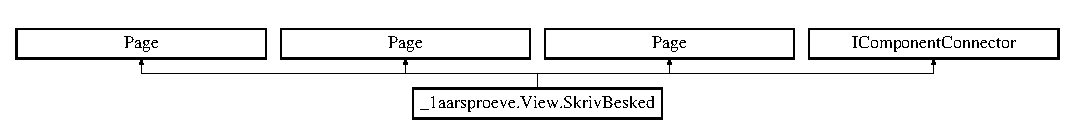
\includegraphics[height=1.365854cm]{class__1aarsproeve_1_1_view_1_1_skriv_besked}
\end{center}
\end{figure}
\subsection*{Public Member Functions}
\begin{DoxyCompactItemize}
\item 
\hypertarget{class__1aarsproeve_1_1_view_1_1_skriv_besked_ae9f6ee3a3c0a435a52b6775f6d50652e}{}void {\bfseries Connect} (int connection\+Id, object target)\label{class__1aarsproeve_1_1_view_1_1_skriv_besked_ae9f6ee3a3c0a435a52b6775f6d50652e}

\item 
\hypertarget{class__1aarsproeve_1_1_view_1_1_skriv_besked_a765af0a076e2e07eb3dedf725247aaa1}{}void {\bfseries Initialize\+Component} ()\label{class__1aarsproeve_1_1_view_1_1_skriv_besked_a765af0a076e2e07eb3dedf725247aaa1}

\end{DoxyCompactItemize}
\subsection*{Protected Member Functions}
\begin{DoxyCompactItemize}
\item 
override void \hyperlink{class__1aarsproeve_1_1_view_1_1_skriv_besked_ab0c5a22e91f5f089078bd5e4c1f9cdfe}{On\+Navigated\+To} (Navigation\+Event\+Args e)
\item 
\hypertarget{class__1aarsproeve_1_1_view_1_1_skriv_besked_a4aac18ef6aef2d31b964c778dd4f0f91}{}override void {\bfseries On\+Navigated\+From} (Navigation\+Event\+Args e)\label{class__1aarsproeve_1_1_view_1_1_skriv_besked_a4aac18ef6aef2d31b964c778dd4f0f91}

\end{DoxyCompactItemize}
\subsection*{Properties}
\begin{DoxyCompactItemize}
\item 
\hyperlink{class__1aarsproeve_1_1_common_1_1_observable_dictionary}{Observable\+Dictionary} \hyperlink{class__1aarsproeve_1_1_view_1_1_skriv_besked_a32c4fc357cdba1138021e257dd545d53}{Default\+View\+Model}\hspace{0.3cm}{\ttfamily  \mbox{[}get\mbox{]}}
\begin{DoxyCompactList}\small\item\em This can be changed to a strongly typed view model. \end{DoxyCompactList}\item 
\hyperlink{class__1aarsproeve_1_1_common_1_1_navigation_helper}{Navigation\+Helper} \hyperlink{class__1aarsproeve_1_1_view_1_1_skriv_besked_ad24c3da26e1cc62ddf5046f96f170dd7}{Navigation\+Helper}\hspace{0.3cm}{\ttfamily  \mbox{[}get\mbox{]}}
\begin{DoxyCompactList}\small\item\em Navigation\+Helper is used on each page to aid in navigation and process lifetime management \end{DoxyCompactList}\end{DoxyCompactItemize}


\subsection{Detailed Description}
A basic page that provides characteristics common to most applications. 



\subsection{Member Function Documentation}
\hypertarget{class__1aarsproeve_1_1_view_1_1_skriv_besked_ab0c5a22e91f5f089078bd5e4c1f9cdfe}{}\index{\+\_\+1aarsproeve\+::\+View\+::\+Skriv\+Besked@{\+\_\+1aarsproeve\+::\+View\+::\+Skriv\+Besked}!On\+Navigated\+To@{On\+Navigated\+To}}
\index{On\+Navigated\+To@{On\+Navigated\+To}!\+\_\+1aarsproeve\+::\+View\+::\+Skriv\+Besked@{\+\_\+1aarsproeve\+::\+View\+::\+Skriv\+Besked}}
\subsubsection[{On\+Navigated\+To}]{\setlength{\rightskip}{0pt plus 5cm}override void \+\_\+1aarsproeve.\+View.\+Skriv\+Besked.\+On\+Navigated\+To (
\begin{DoxyParamCaption}
\item[{Navigation\+Event\+Args}]{e}
\end{DoxyParamCaption}
)\hspace{0.3cm}{\ttfamily [inline]}, {\ttfamily [protected]}}\label{class__1aarsproeve_1_1_view_1_1_skriv_besked_ab0c5a22e91f5f089078bd5e4c1f9cdfe}
The methods provided in this section are simply used to allow Navigation\+Helper to respond to the page\textquotesingle{}s navigation methods.

Page specific logic should be placed in event handlers for the Grid\+C\+S.\+Common.\+Navigation\+Helper.\+Load\+State and Grid\+C\+S.\+Common.\+Navigation\+Helper.\+Save\+State. The navigation parameter is available in the Load\+State method in addition to page state preserved during an earlier session. 

\subsection{Property Documentation}
\hypertarget{class__1aarsproeve_1_1_view_1_1_skriv_besked_a32c4fc357cdba1138021e257dd545d53}{}\index{\+\_\+1aarsproeve\+::\+View\+::\+Skriv\+Besked@{\+\_\+1aarsproeve\+::\+View\+::\+Skriv\+Besked}!Default\+View\+Model@{Default\+View\+Model}}
\index{Default\+View\+Model@{Default\+View\+Model}!\+\_\+1aarsproeve\+::\+View\+::\+Skriv\+Besked@{\+\_\+1aarsproeve\+::\+View\+::\+Skriv\+Besked}}
\subsubsection[{Default\+View\+Model}]{\setlength{\rightskip}{0pt plus 5cm}{\bf Observable\+Dictionary} \+\_\+1aarsproeve.\+View.\+Skriv\+Besked.\+Default\+View\+Model\hspace{0.3cm}{\ttfamily [get]}}\label{class__1aarsproeve_1_1_view_1_1_skriv_besked_a32c4fc357cdba1138021e257dd545d53}


This can be changed to a strongly typed view model. 

\hypertarget{class__1aarsproeve_1_1_view_1_1_skriv_besked_ad24c3da26e1cc62ddf5046f96f170dd7}{}\index{\+\_\+1aarsproeve\+::\+View\+::\+Skriv\+Besked@{\+\_\+1aarsproeve\+::\+View\+::\+Skriv\+Besked}!Navigation\+Helper@{Navigation\+Helper}}
\index{Navigation\+Helper@{Navigation\+Helper}!\+\_\+1aarsproeve\+::\+View\+::\+Skriv\+Besked@{\+\_\+1aarsproeve\+::\+View\+::\+Skriv\+Besked}}
\subsubsection[{Navigation\+Helper}]{\setlength{\rightskip}{0pt plus 5cm}{\bf Navigation\+Helper} \+\_\+1aarsproeve.\+View.\+Skriv\+Besked.\+Navigation\+Helper\hspace{0.3cm}{\ttfamily [get]}}\label{class__1aarsproeve_1_1_view_1_1_skriv_besked_ad24c3da26e1cc62ddf5046f96f170dd7}


Navigation\+Helper is used on each page to aid in navigation and process lifetime management 



The documentation for this class was generated from the following files\+:\begin{DoxyCompactItemize}
\item 
C\+:/\+Users/\+Daniel\+Winther/\+Documents/\+Git\+Hub/1-\/aarsproeve/1aarsproeve/1aarsproeve/obj/\+Debug/\+View/Skriv\+Besked.\+g.\+cs\item 
C\+:/\+Users/\+Daniel\+Winther/\+Documents/\+Git\+Hub/1-\/aarsproeve/1aarsproeve/1aarsproeve/obj/\+Debug/\+View/Skriv\+Besked.\+g.\+i.\+cs\item 
C\+:/\+Users/\+Daniel\+Winther/\+Documents/\+Git\+Hub/1-\/aarsproeve/1aarsproeve/1aarsproeve/\+View/Skriv\+Besked.\+xaml.\+cs\end{DoxyCompactItemize}

\hypertarget{class__1aarsproeve_1_1_common_1_1_suspension_manager_exception}{}\section{\+\_\+1aarsproeve.\+Common.\+Suspension\+Manager\+Exception Class Reference}
\label{class__1aarsproeve_1_1_common_1_1_suspension_manager_exception}\index{\+\_\+1aarsproeve.\+Common.\+Suspension\+Manager\+Exception@{\+\_\+1aarsproeve.\+Common.\+Suspension\+Manager\+Exception}}
Inheritance diagram for \+\_\+1aarsproeve.\+Common.\+Suspension\+Manager\+Exception\+:\begin{figure}[H]
\begin{center}
\leavevmode
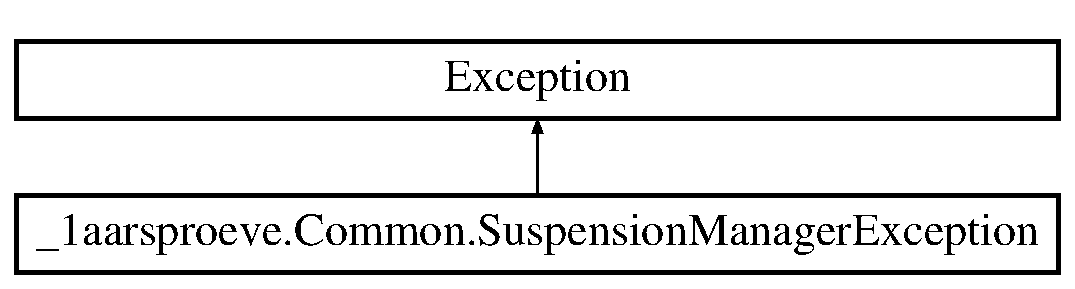
\includegraphics[height=2.000000cm]{class__1aarsproeve_1_1_common_1_1_suspension_manager_exception}
\end{center}
\end{figure}
\subsection*{Public Member Functions}
\begin{DoxyCompactItemize}
\item 
\hypertarget{class__1aarsproeve_1_1_common_1_1_suspension_manager_exception_a7beaead1dc1988f760ae8913a5b2b4c8}{}{\bfseries Suspension\+Manager\+Exception} (Exception e)\label{class__1aarsproeve_1_1_common_1_1_suspension_manager_exception_a7beaead1dc1988f760ae8913a5b2b4c8}

\end{DoxyCompactItemize}


The documentation for this class was generated from the following file\+:\begin{DoxyCompactItemize}
\item 
Documents/\+Git\+Hub/1-\/aarsproeve/1aarsproeve/1aarsproeve/\+Common/Suspension\+Manager.\+cs\end{DoxyCompactItemize}

\hypertarget{class__1aarsproeve_web_service_1_1_areas_1_1_help_page_1_1_text_sample}{}\section{\+\_\+1aarsproeve\+Web\+Service.\+Areas.\+Help\+Page.\+Text\+Sample Class Reference}
\label{class__1aarsproeve_web_service_1_1_areas_1_1_help_page_1_1_text_sample}\index{\+\_\+1aarsproeve\+Web\+Service.\+Areas.\+Help\+Page.\+Text\+Sample@{\+\_\+1aarsproeve\+Web\+Service.\+Areas.\+Help\+Page.\+Text\+Sample}}


This represents a preformatted text sample on the help page. There\textquotesingle{}s a display template named \hyperlink{class__1aarsproeve_web_service_1_1_areas_1_1_help_page_1_1_text_sample}{Text\+Sample} associated with this class.  


\subsection*{Public Member Functions}
\begin{DoxyCompactItemize}
\item 
\hypertarget{class__1aarsproeve_web_service_1_1_areas_1_1_help_page_1_1_text_sample_a543e2aa253bd24774b7b5d50aa6d1770}{}{\bfseries Text\+Sample} (string text)\label{class__1aarsproeve_web_service_1_1_areas_1_1_help_page_1_1_text_sample_a543e2aa253bd24774b7b5d50aa6d1770}

\item 
\hypertarget{class__1aarsproeve_web_service_1_1_areas_1_1_help_page_1_1_text_sample_a1d5523486e9a0c505aa78bc05ea0b50c}{}override bool {\bfseries Equals} (object obj)\label{class__1aarsproeve_web_service_1_1_areas_1_1_help_page_1_1_text_sample_a1d5523486e9a0c505aa78bc05ea0b50c}

\item 
\hypertarget{class__1aarsproeve_web_service_1_1_areas_1_1_help_page_1_1_text_sample_ad37edf7bad0bd3016c03b96bcc26e8ad}{}override int {\bfseries Get\+Hash\+Code} ()\label{class__1aarsproeve_web_service_1_1_areas_1_1_help_page_1_1_text_sample_ad37edf7bad0bd3016c03b96bcc26e8ad}

\item 
\hypertarget{class__1aarsproeve_web_service_1_1_areas_1_1_help_page_1_1_text_sample_a832d14e2ad55878eec7de411c165c2fc}{}override string {\bfseries To\+String} ()\label{class__1aarsproeve_web_service_1_1_areas_1_1_help_page_1_1_text_sample_a832d14e2ad55878eec7de411c165c2fc}

\end{DoxyCompactItemize}
\subsection*{Properties}
\begin{DoxyCompactItemize}
\item 
\hypertarget{class__1aarsproeve_web_service_1_1_areas_1_1_help_page_1_1_text_sample_af691a0f912794fd1c606e7d0fa73dbee}{}string {\bfseries Text}\hspace{0.3cm}{\ttfamily  \mbox{[}get\mbox{]}}\label{class__1aarsproeve_web_service_1_1_areas_1_1_help_page_1_1_text_sample_af691a0f912794fd1c606e7d0fa73dbee}

\end{DoxyCompactItemize}


\subsection{Detailed Description}
This represents a preformatted text sample on the help page. There\textquotesingle{}s a display template named \hyperlink{class__1aarsproeve_web_service_1_1_areas_1_1_help_page_1_1_text_sample}{Text\+Sample} associated with this class. 



The documentation for this class was generated from the following file\+:\begin{DoxyCompactItemize}
\item 
Documents/\+Git\+Hub/1-\/aarsproeve/1aarsproeve/1aarsproeve\+Web\+Service/\+Areas/\+Help\+Page/\+Sample\+Generation/Text\+Sample.\+cs\end{DoxyCompactItemize}

\hypertarget{class__1aarsproeve_1_1_view_1_1_vagtplan}{}\section{\+\_\+1aarsproeve.\+View.\+Vagtplan Class Reference}
\label{class__1aarsproeve_1_1_view_1_1_vagtplan}\index{\+\_\+1aarsproeve.\+View.\+Vagtplan@{\+\_\+1aarsproeve.\+View.\+Vagtplan}}


A basic page that provides characteristics common to most applications.  


Inheritance diagram for \+\_\+1aarsproeve.\+View.\+Vagtplan\+:\begin{figure}[H]
\begin{center}
\leavevmode
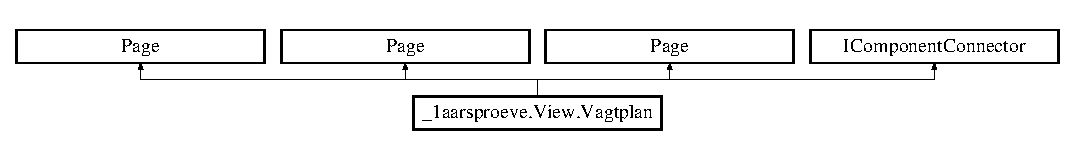
\includegraphics[height=1.513514cm]{class__1aarsproeve_1_1_view_1_1_vagtplan}
\end{center}
\end{figure}
\subsection*{Public Member Functions}
\begin{DoxyCompactItemize}
\item 
\hypertarget{class__1aarsproeve_1_1_view_1_1_vagtplan_ab5463d2d22c5daef5e72b0db649f28d2}{}void {\bfseries Connect} (int connection\+Id, object target)\label{class__1aarsproeve_1_1_view_1_1_vagtplan_ab5463d2d22c5daef5e72b0db649f28d2}

\item 
\hypertarget{class__1aarsproeve_1_1_view_1_1_vagtplan_a8a8cf75ef052a6e0a568fd355a812f16}{}void {\bfseries Initialize\+Component} ()\label{class__1aarsproeve_1_1_view_1_1_vagtplan_a8a8cf75ef052a6e0a568fd355a812f16}

\end{DoxyCompactItemize}
\subsection*{Protected Member Functions}
\begin{DoxyCompactItemize}
\item 
override void \hyperlink{class__1aarsproeve_1_1_view_1_1_vagtplan_a527b20b4c4b466d22919195324fe2600}{On\+Navigated\+To} (Navigation\+Event\+Args e)
\item 
\hypertarget{class__1aarsproeve_1_1_view_1_1_vagtplan_a0bc36f20e2eec79bd26ca4701a42bcec}{}override void {\bfseries On\+Navigated\+From} (Navigation\+Event\+Args e)\label{class__1aarsproeve_1_1_view_1_1_vagtplan_a0bc36f20e2eec79bd26ca4701a42bcec}

\end{DoxyCompactItemize}
\subsection*{Properties}
\begin{DoxyCompactItemize}
\item 
\hyperlink{class__1aarsproeve_1_1_common_1_1_observable_dictionary}{Observable\+Dictionary} \hyperlink{class__1aarsproeve_1_1_view_1_1_vagtplan_aa886f262e9d0680645f45daa22bd473a}{Default\+View\+Model}\hspace{0.3cm}{\ttfamily  \mbox{[}get\mbox{]}}
\begin{DoxyCompactList}\small\item\em This can be changed to a strongly typed view model. \end{DoxyCompactList}\item 
\hyperlink{class__1aarsproeve_1_1_common_1_1_navigation_helper}{Navigation\+Helper} \hyperlink{class__1aarsproeve_1_1_view_1_1_vagtplan_a8821ea381132cfc4259a782a59201134}{Navigation\+Helper}\hspace{0.3cm}{\ttfamily  \mbox{[}get\mbox{]}}
\begin{DoxyCompactList}\small\item\em Navigation\+Helper is used on each page to aid in navigation and process lifetime management \end{DoxyCompactList}\end{DoxyCompactItemize}


\subsection{Detailed Description}
A basic page that provides characteristics common to most applications. 



\subsection{Member Function Documentation}
\hypertarget{class__1aarsproeve_1_1_view_1_1_vagtplan_a527b20b4c4b466d22919195324fe2600}{}\index{\+\_\+1aarsproeve\+::\+View\+::\+Vagtplan@{\+\_\+1aarsproeve\+::\+View\+::\+Vagtplan}!On\+Navigated\+To@{On\+Navigated\+To}}
\index{On\+Navigated\+To@{On\+Navigated\+To}!\+\_\+1aarsproeve\+::\+View\+::\+Vagtplan@{\+\_\+1aarsproeve\+::\+View\+::\+Vagtplan}}
\subsubsection[{On\+Navigated\+To}]{\setlength{\rightskip}{0pt plus 5cm}override void \+\_\+1aarsproeve.\+View.\+Vagtplan.\+On\+Navigated\+To (
\begin{DoxyParamCaption}
\item[{Navigation\+Event\+Args}]{e}
\end{DoxyParamCaption}
)\hspace{0.3cm}{\ttfamily [inline]}, {\ttfamily [protected]}}\label{class__1aarsproeve_1_1_view_1_1_vagtplan_a527b20b4c4b466d22919195324fe2600}
The methods provided in this section are simply used to allow Navigation\+Helper to respond to the page\textquotesingle{}s navigation methods.

Page specific logic should be placed in event handlers for the Grid\+C\+S.\+Common.\+Navigation\+Helper.\+Load\+State and Grid\+C\+S.\+Common.\+Navigation\+Helper.\+Save\+State. The navigation parameter is available in the Load\+State method in addition to page state preserved during an earlier session. 

\subsection{Property Documentation}
\hypertarget{class__1aarsproeve_1_1_view_1_1_vagtplan_aa886f262e9d0680645f45daa22bd473a}{}\index{\+\_\+1aarsproeve\+::\+View\+::\+Vagtplan@{\+\_\+1aarsproeve\+::\+View\+::\+Vagtplan}!Default\+View\+Model@{Default\+View\+Model}}
\index{Default\+View\+Model@{Default\+View\+Model}!\+\_\+1aarsproeve\+::\+View\+::\+Vagtplan@{\+\_\+1aarsproeve\+::\+View\+::\+Vagtplan}}
\subsubsection[{Default\+View\+Model}]{\setlength{\rightskip}{0pt plus 5cm}{\bf Observable\+Dictionary} \+\_\+1aarsproeve.\+View.\+Vagtplan.\+Default\+View\+Model\hspace{0.3cm}{\ttfamily [get]}}\label{class__1aarsproeve_1_1_view_1_1_vagtplan_aa886f262e9d0680645f45daa22bd473a}


This can be changed to a strongly typed view model. 

\hypertarget{class__1aarsproeve_1_1_view_1_1_vagtplan_a8821ea381132cfc4259a782a59201134}{}\index{\+\_\+1aarsproeve\+::\+View\+::\+Vagtplan@{\+\_\+1aarsproeve\+::\+View\+::\+Vagtplan}!Navigation\+Helper@{Navigation\+Helper}}
\index{Navigation\+Helper@{Navigation\+Helper}!\+\_\+1aarsproeve\+::\+View\+::\+Vagtplan@{\+\_\+1aarsproeve\+::\+View\+::\+Vagtplan}}
\subsubsection[{Navigation\+Helper}]{\setlength{\rightskip}{0pt plus 5cm}{\bf Navigation\+Helper} \+\_\+1aarsproeve.\+View.\+Vagtplan.\+Navigation\+Helper\hspace{0.3cm}{\ttfamily [get]}}\label{class__1aarsproeve_1_1_view_1_1_vagtplan_a8821ea381132cfc4259a782a59201134}


Navigation\+Helper is used on each page to aid in navigation and process lifetime management 



The documentation for this class was generated from the following files\+:\begin{DoxyCompactItemize}
\item 
C\+:/\+Users/\+Daniel\+Winther/\+Documents/\+Git\+Hub/1-\/aarsproeve/1aarsproeve/1aarsproeve/obj/\+Debug/\+View/Vagtplan.\+g.\+cs\item 
C\+:/\+Users/\+Daniel\+Winther/\+Documents/\+Git\+Hub/1-\/aarsproeve/1aarsproeve/1aarsproeve/obj/\+Debug/\+View/Vagtplan.\+g.\+i.\+cs\item 
C\+:/\+Users/\+Daniel\+Winther/\+Documents/\+Git\+Hub/1-\/aarsproeve/1aarsproeve/1aarsproeve/\+View/Vagtplan.\+xaml.\+cs\end{DoxyCompactItemize}

\hypertarget{class__1aarsproeve_1_1_view_model_1_1_vagtplan_view_model}{}\section{\+\_\+1aarsproeve.\+View\+Model.\+Vagtplan\+View\+Model Class Reference}
\label{class__1aarsproeve_1_1_view_model_1_1_vagtplan_view_model}\index{\+\_\+1aarsproeve.\+View\+Model.\+Vagtplan\+View\+Model@{\+\_\+1aarsproeve.\+View\+Model.\+Vagtplan\+View\+Model}}
\subsection*{Public Member Functions}
\begin{DoxyCompactItemize}
\item 
\hypertarget{class__1aarsproeve_1_1_view_model_1_1_vagtplan_view_model_a584ab28ecfddbb2248d7b55a3ed10a34}{}void {\bfseries Nuvaerende\+Ugedag} (Solid\+Color\+Brush brush, Solid\+Color\+Brush brush\+Original)\label{class__1aarsproeve_1_1_view_model_1_1_vagtplan_view_model_a584ab28ecfddbb2248d7b55a3ed10a34}

\item 
\hypertarget{class__1aarsproeve_1_1_view_model_1_1_vagtplan_view_model_a5e3b5ba40e74748da6c018f8547d8baa}{}void {\bfseries Find\+Ugenummer} (string kultur\+Info)\label{class__1aarsproeve_1_1_view_model_1_1_vagtplan_view_model_a5e3b5ba40e74748da6c018f8547d8baa}

\item 
\hypertarget{class__1aarsproeve_1_1_view_model_1_1_vagtplan_view_model_a8b8894a622f861e335c3e171a4ba93bc}{}Date\+Time {\bfseries Foerste\+Dag\+Paa\+Uge} (int uge\+Paa\+Aaret)\label{class__1aarsproeve_1_1_view_model_1_1_vagtplan_view_model_a8b8894a622f861e335c3e171a4ba93bc}

\item 
\hypertarget{class__1aarsproeve_1_1_view_model_1_1_vagtplan_view_model_ad4620a85449f88c843d594dfb7e2f5fa}{}void {\bfseries Initialiser\+Ugedage} ()\label{class__1aarsproeve_1_1_view_model_1_1_vagtplan_view_model_ad4620a85449f88c843d594dfb7e2f5fa}

\item 
\hypertarget{class__1aarsproeve_1_1_view_model_1_1_vagtplan_view_model_a5616979ee0bb0fe1904d965f2b688560}{}void {\bfseries Initialiser\+Ansatte} ()\label{class__1aarsproeve_1_1_view_model_1_1_vagtplan_view_model_a5616979ee0bb0fe1904d965f2b688560}

\item 
\hypertarget{class__1aarsproeve_1_1_view_model_1_1_vagtplan_view_model_a1e49e7514900058b5cd36e4991e08b23}{}void {\bfseries Alle\+Vagter} ()\label{class__1aarsproeve_1_1_view_model_1_1_vagtplan_view_model_a1e49e7514900058b5cd36e4991e08b23}

\item 
\hypertarget{class__1aarsproeve_1_1_view_model_1_1_vagtplan_view_model_aac01e39a92807c54f6718d4be4aeabc2}{}void {\bfseries Frie\+Vagter} ()\label{class__1aarsproeve_1_1_view_model_1_1_vagtplan_view_model_aac01e39a92807c54f6718d4be4aeabc2}

\item 
\hypertarget{class__1aarsproeve_1_1_view_model_1_1_vagtplan_view_model_a94fda6c42d4819fa2af8af5e2c22eff1}{}void {\bfseries Mine\+Vagter} ()\label{class__1aarsproeve_1_1_view_model_1_1_vagtplan_view_model_a94fda6c42d4819fa2af8af5e2c22eff1}

\item 
\hypertarget{class__1aarsproeve_1_1_view_model_1_1_vagtplan_view_model_a543ec6d690130a11d074bc58ba9f1552}{}void {\bfseries Log\+Ud} ()\label{class__1aarsproeve_1_1_view_model_1_1_vagtplan_view_model_a543ec6d690130a11d074bc58ba9f1552}

\end{DoxyCompactItemize}
\subsection*{Properties}
\begin{DoxyCompactItemize}
\item 
\hypertarget{class__1aarsproeve_1_1_view_model_1_1_vagtplan_view_model_aa5e675ea6389cdc802698037ced2e091}{}Application\+Data\+Container {\bfseries Setting}\hspace{0.3cm}{\ttfamily  \mbox{[}get, set\mbox{]}}\label{class__1aarsproeve_1_1_view_model_1_1_vagtplan_view_model_aa5e675ea6389cdc802698037ced2e091}

\item 
\hypertarget{class__1aarsproeve_1_1_view_model_1_1_vagtplan_view_model_a2bb8421c370d9ff0ff1776a1c239ba4e}{}string {\bfseries Brugernavn}\hspace{0.3cm}{\ttfamily  \mbox{[}get, set\mbox{]}}\label{class__1aarsproeve_1_1_view_model_1_1_vagtplan_view_model_a2bb8421c370d9ff0ff1776a1c239ba4e}

\item 
\hypertarget{class__1aarsproeve_1_1_view_model_1_1_vagtplan_view_model_ad7b9435c1500a21d04418bedeead2094}{}Brush {\bfseries Mandag\+Farve}\hspace{0.3cm}{\ttfamily  \mbox{[}get, set\mbox{]}}\label{class__1aarsproeve_1_1_view_model_1_1_vagtplan_view_model_ad7b9435c1500a21d04418bedeead2094}

\item 
\hypertarget{class__1aarsproeve_1_1_view_model_1_1_vagtplan_view_model_adc98e55c2f01916b7581f1ef865a70bc}{}Brush {\bfseries Tirsdag\+Farve}\hspace{0.3cm}{\ttfamily  \mbox{[}get, set\mbox{]}}\label{class__1aarsproeve_1_1_view_model_1_1_vagtplan_view_model_adc98e55c2f01916b7581f1ef865a70bc}

\item 
\hypertarget{class__1aarsproeve_1_1_view_model_1_1_vagtplan_view_model_a3c463aaf64f3e35e910640a29969943d}{}Brush {\bfseries Onsdag\+Farve}\hspace{0.3cm}{\ttfamily  \mbox{[}get, set\mbox{]}}\label{class__1aarsproeve_1_1_view_model_1_1_vagtplan_view_model_a3c463aaf64f3e35e910640a29969943d}

\item 
\hypertarget{class__1aarsproeve_1_1_view_model_1_1_vagtplan_view_model_a88d17bbfb35c27d773321581f4cfd5df}{}Brush {\bfseries Torsdag\+Farve}\hspace{0.3cm}{\ttfamily  \mbox{[}get, set\mbox{]}}\label{class__1aarsproeve_1_1_view_model_1_1_vagtplan_view_model_a88d17bbfb35c27d773321581f4cfd5df}

\item 
\hypertarget{class__1aarsproeve_1_1_view_model_1_1_vagtplan_view_model_a77eb2c412d3a8adb1a46aad714bae471}{}Brush {\bfseries Fredag\+Farve}\hspace{0.3cm}{\ttfamily  \mbox{[}get, set\mbox{]}}\label{class__1aarsproeve_1_1_view_model_1_1_vagtplan_view_model_a77eb2c412d3a8adb1a46aad714bae471}

\item 
\hypertarget{class__1aarsproeve_1_1_view_model_1_1_vagtplan_view_model_a185e3bddfb80d3f012af638b27bbf99a}{}Brush {\bfseries Loerdag\+Farve}\hspace{0.3cm}{\ttfamily  \mbox{[}get, set\mbox{]}}\label{class__1aarsproeve_1_1_view_model_1_1_vagtplan_view_model_a185e3bddfb80d3f012af638b27bbf99a}

\item 
\hypertarget{class__1aarsproeve_1_1_view_model_1_1_vagtplan_view_model_aa6afb148e3e73f41c510862b157affb0}{}Brush {\bfseries Soendag\+Farve}\hspace{0.3cm}{\ttfamily  \mbox{[}get, set\mbox{]}}\label{class__1aarsproeve_1_1_view_model_1_1_vagtplan_view_model_aa6afb148e3e73f41c510862b157affb0}

\item 
\hypertarget{class__1aarsproeve_1_1_view_model_1_1_vagtplan_view_model_a34eaf9433fb67fa445834864cc4117d4}{}int {\bfseries Ugenummer}\hspace{0.3cm}{\ttfamily  \mbox{[}get, set\mbox{]}}\label{class__1aarsproeve_1_1_view_model_1_1_vagtplan_view_model_a34eaf9433fb67fa445834864cc4117d4}

\item 
\hypertarget{class__1aarsproeve_1_1_view_model_1_1_vagtplan_view_model_aa78a723e55f22d0579a6a5cc0086a2fc}{}string {\bfseries Mandag}\hspace{0.3cm}{\ttfamily  \mbox{[}get, set\mbox{]}}\label{class__1aarsproeve_1_1_view_model_1_1_vagtplan_view_model_aa78a723e55f22d0579a6a5cc0086a2fc}

\item 
\hypertarget{class__1aarsproeve_1_1_view_model_1_1_vagtplan_view_model_a504d0377b323ec2af99d27a0b586924a}{}string {\bfseries Tirsdag}\hspace{0.3cm}{\ttfamily  \mbox{[}get, set\mbox{]}}\label{class__1aarsproeve_1_1_view_model_1_1_vagtplan_view_model_a504d0377b323ec2af99d27a0b586924a}

\item 
\hypertarget{class__1aarsproeve_1_1_view_model_1_1_vagtplan_view_model_a4d544dfd8109650066d5e9d25642c352}{}string {\bfseries Onsdag}\hspace{0.3cm}{\ttfamily  \mbox{[}get, set\mbox{]}}\label{class__1aarsproeve_1_1_view_model_1_1_vagtplan_view_model_a4d544dfd8109650066d5e9d25642c352}

\item 
\hypertarget{class__1aarsproeve_1_1_view_model_1_1_vagtplan_view_model_a8ae90390ac0ead14c7542bb1b735ec75}{}string {\bfseries Torsdag}\hspace{0.3cm}{\ttfamily  \mbox{[}get, set\mbox{]}}\label{class__1aarsproeve_1_1_view_model_1_1_vagtplan_view_model_a8ae90390ac0ead14c7542bb1b735ec75}

\item 
\hypertarget{class__1aarsproeve_1_1_view_model_1_1_vagtplan_view_model_a7da74e228f974d9756603957477f65da}{}string {\bfseries Fredag}\hspace{0.3cm}{\ttfamily  \mbox{[}get, set\mbox{]}}\label{class__1aarsproeve_1_1_view_model_1_1_vagtplan_view_model_a7da74e228f974d9756603957477f65da}

\item 
\hypertarget{class__1aarsproeve_1_1_view_model_1_1_vagtplan_view_model_aa7572363a0fffba490fb61060c922594}{}string {\bfseries Loerdag}\hspace{0.3cm}{\ttfamily  \mbox{[}get, set\mbox{]}}\label{class__1aarsproeve_1_1_view_model_1_1_vagtplan_view_model_aa7572363a0fffba490fb61060c922594}

\item 
\hypertarget{class__1aarsproeve_1_1_view_model_1_1_vagtplan_view_model_abdd4c1e28095f4c2660a5ad71bab51ee}{}string {\bfseries Soendag}\hspace{0.3cm}{\ttfamily  \mbox{[}get, set\mbox{]}}\label{class__1aarsproeve_1_1_view_model_1_1_vagtplan_view_model_abdd4c1e28095f4c2660a5ad71bab51ee}

\item 
\hypertarget{class__1aarsproeve_1_1_view_model_1_1_vagtplan_view_model_a2c5e8d56bdec0db35b7e4c4d3f5a8bcb}{}Observable\+Collection$<$ Ugedage $>$ {\bfseries Ugedage\+Collection}\hspace{0.3cm}{\ttfamily  \mbox{[}get, set\mbox{]}}\label{class__1aarsproeve_1_1_view_model_1_1_vagtplan_view_model_a2c5e8d56bdec0db35b7e4c4d3f5a8bcb}

\item 
\hypertarget{class__1aarsproeve_1_1_view_model_1_1_vagtplan_view_model_a9ff1365b62555d179cf34a5e11a6d5fc}{}I\+Command {\bfseries Alle\+Vagter\+Command}\hspace{0.3cm}{\ttfamily  \mbox{[}get, set\mbox{]}}\label{class__1aarsproeve_1_1_view_model_1_1_vagtplan_view_model_a9ff1365b62555d179cf34a5e11a6d5fc}

\item 
\hypertarget{class__1aarsproeve_1_1_view_model_1_1_vagtplan_view_model_ac17a43f67342176e4a94bea072876d9c}{}I\+Command {\bfseries Frie\+Vagter\+Command}\hspace{0.3cm}{\ttfamily  \mbox{[}get, set\mbox{]}}\label{class__1aarsproeve_1_1_view_model_1_1_vagtplan_view_model_ac17a43f67342176e4a94bea072876d9c}

\item 
\hypertarget{class__1aarsproeve_1_1_view_model_1_1_vagtplan_view_model_abded4dcbd3699986defbf179b9d52001}{}I\+Command {\bfseries Mine\+Vagter\+Command}\hspace{0.3cm}{\ttfamily  \mbox{[}get, set\mbox{]}}\label{class__1aarsproeve_1_1_view_model_1_1_vagtplan_view_model_abded4dcbd3699986defbf179b9d52001}

\item 
\hypertarget{class__1aarsproeve_1_1_view_model_1_1_vagtplan_view_model_aadc2e0233944328d65644e49b449f89b}{}I\+Command {\bfseries Log\+Ud\+Command}\hspace{0.3cm}{\ttfamily  \mbox{[}get, set\mbox{]}}\label{class__1aarsproeve_1_1_view_model_1_1_vagtplan_view_model_aadc2e0233944328d65644e49b449f89b}

\end{DoxyCompactItemize}


The documentation for this class was generated from the following file\+:\begin{DoxyCompactItemize}
\item 
Documents/\+Git\+Hub/1-\/aarsproeve/1aarsproeve/1aarsproeve/\+View\+Model/Vagtplan\+View\+Model.\+cs\end{DoxyCompactItemize}

\hypertarget{class__1aarsproeve_web_service_1_1_controllers_1_1_values_controller}{}\section{\+\_\+1aarsproeve\+Web\+Service.\+Controllers.\+Values\+Controller Class Reference}
\label{class__1aarsproeve_web_service_1_1_controllers_1_1_values_controller}\index{\+\_\+1aarsproeve\+Web\+Service.\+Controllers.\+Values\+Controller@{\+\_\+1aarsproeve\+Web\+Service.\+Controllers.\+Values\+Controller}}
Inheritance diagram for \+\_\+1aarsproeve\+Web\+Service.\+Controllers.\+Values\+Controller\+:\begin{figure}[H]
\begin{center}
\leavevmode
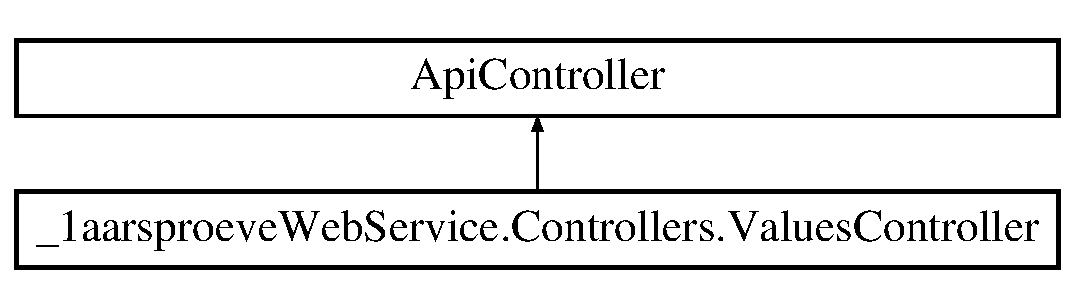
\includegraphics[height=2.000000cm]{class__1aarsproeve_web_service_1_1_controllers_1_1_values_controller}
\end{center}
\end{figure}
\subsection*{Public Member Functions}
\begin{DoxyCompactItemize}
\item 
\hypertarget{class__1aarsproeve_web_service_1_1_controllers_1_1_values_controller_a6aabdf6d41689230f8c9ac16bd6e0cf2}{}I\+Enumerable$<$ string $>$ {\bfseries Get} ()\label{class__1aarsproeve_web_service_1_1_controllers_1_1_values_controller_a6aabdf6d41689230f8c9ac16bd6e0cf2}

\item 
\hypertarget{class__1aarsproeve_web_service_1_1_controllers_1_1_values_controller_a23709bd2085124a4a9523ee83f3f2458}{}string {\bfseries Get} (int id)\label{class__1aarsproeve_web_service_1_1_controllers_1_1_values_controller_a23709bd2085124a4a9523ee83f3f2458}

\item 
\hypertarget{class__1aarsproeve_web_service_1_1_controllers_1_1_values_controller_a67e206660305cb8c2e3245c6cbe137d2}{}void {\bfseries Post} (\mbox{[}From\+Body\mbox{]}string value)\label{class__1aarsproeve_web_service_1_1_controllers_1_1_values_controller_a67e206660305cb8c2e3245c6cbe137d2}

\item 
\hypertarget{class__1aarsproeve_web_service_1_1_controllers_1_1_values_controller_a050db0929ea30dc0e8ad7a296ba7f348}{}void {\bfseries Put} (int id, \mbox{[}From\+Body\mbox{]}string value)\label{class__1aarsproeve_web_service_1_1_controllers_1_1_values_controller_a050db0929ea30dc0e8ad7a296ba7f348}

\item 
\hypertarget{class__1aarsproeve_web_service_1_1_controllers_1_1_values_controller_aea45aefd356d052c838878691e7fb645}{}void {\bfseries Delete} (int id)\label{class__1aarsproeve_web_service_1_1_controllers_1_1_values_controller_aea45aefd356d052c838878691e7fb645}

\end{DoxyCompactItemize}


The documentation for this class was generated from the following file\+:\begin{DoxyCompactItemize}
\item 
C\+:/\+Users/\+Daniel\+Winther/\+Documents/\+Git\+Hub/1-\/aarsproeve/1aarsproeve/1aarsproeve\+Web\+Service/\+Controllers/Values\+Controller.\+cs\end{DoxyCompactItemize}

\hypertarget{class__1aarsproeve_web_service_1_1_web_api_application}{}\section{\+\_\+1aarsproeve\+Web\+Service.\+Web\+Api\+Application Class Reference}
\label{class__1aarsproeve_web_service_1_1_web_api_application}\index{\+\_\+1aarsproeve\+Web\+Service.\+Web\+Api\+Application@{\+\_\+1aarsproeve\+Web\+Service.\+Web\+Api\+Application}}
Inheritance diagram for \+\_\+1aarsproeve\+Web\+Service.\+Web\+Api\+Application\+:\begin{figure}[H]
\begin{center}
\leavevmode
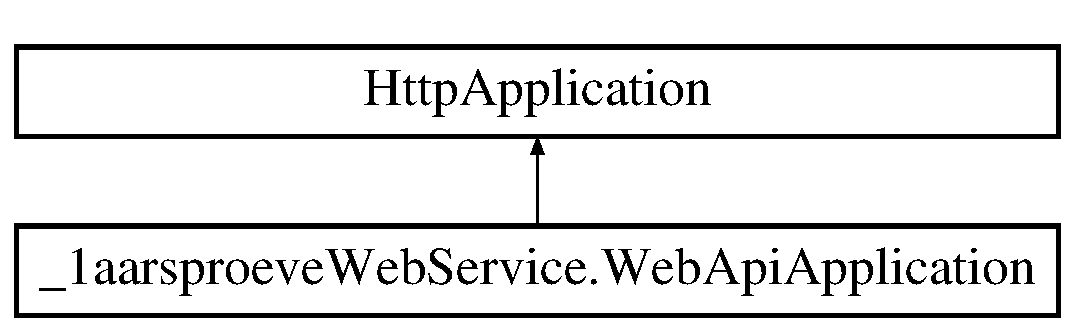
\includegraphics[height=2.000000cm]{class__1aarsproeve_web_service_1_1_web_api_application}
\end{center}
\end{figure}
\subsection*{Protected Member Functions}
\begin{DoxyCompactItemize}
\item 
\hypertarget{class__1aarsproeve_web_service_1_1_web_api_application_a4df9555d507ebda395e42ae2f0b20acf}{}void {\bfseries Application\+\_\+\+Start} ()\label{class__1aarsproeve_web_service_1_1_web_api_application_a4df9555d507ebda395e42ae2f0b20acf}

\end{DoxyCompactItemize}


The documentation for this class was generated from the following file\+:\begin{DoxyCompactItemize}
\item 
C\+:/\+Users/\+Daniel\+Winther/\+Documents/\+Git\+Hub/1-\/aarsproeve/1aarsproeve/1aarsproeve\+Web\+Service/Global.\+asax.\+cs\end{DoxyCompactItemize}

\hypertarget{class__1aarsproeve_web_service_1_1_areas_1_1_help_page_1_1_xml_documentation_provider}{}\section{\+\_\+1aarsproeve\+Web\+Service.\+Areas.\+Help\+Page.\+Xml\+Documentation\+Provider Class Reference}
\label{class__1aarsproeve_web_service_1_1_areas_1_1_help_page_1_1_xml_documentation_provider}\index{\+\_\+1aarsproeve\+Web\+Service.\+Areas.\+Help\+Page.\+Xml\+Documentation\+Provider@{\+\_\+1aarsproeve\+Web\+Service.\+Areas.\+Help\+Page.\+Xml\+Documentation\+Provider}}


A custom I\+Documentation\+Provider that reads the A\+P\+I documentation from an X\+M\+L documentation file.  


Inheritance diagram for \+\_\+1aarsproeve\+Web\+Service.\+Areas.\+Help\+Page.\+Xml\+Documentation\+Provider\+:\begin{figure}[H]
\begin{center}
\leavevmode
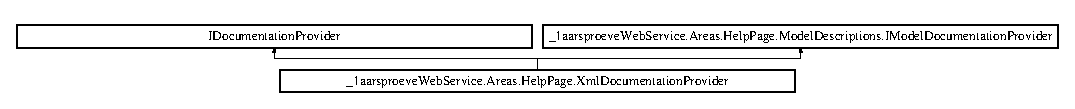
\includegraphics[height=1.021898cm]{class__1aarsproeve_web_service_1_1_areas_1_1_help_page_1_1_xml_documentation_provider}
\end{center}
\end{figure}
\subsection*{Public Member Functions}
\begin{DoxyCompactItemize}
\item 
\hyperlink{class__1aarsproeve_web_service_1_1_areas_1_1_help_page_1_1_xml_documentation_provider_a9756d09583c49feedecafd710687979a}{Xml\+Documentation\+Provider} (string document\+Path)
\begin{DoxyCompactList}\small\item\em Initializes a new instance of the \hyperlink{class__1aarsproeve_web_service_1_1_areas_1_1_help_page_1_1_xml_documentation_provider}{Xml\+Documentation\+Provider} class. \end{DoxyCompactList}\item 
\hypertarget{class__1aarsproeve_web_service_1_1_areas_1_1_help_page_1_1_xml_documentation_provider_aa8ff5033f41ffc32d11bade7e90f2b02}{}string {\bfseries Get\+Documentation} (Http\+Controller\+Descriptor controller\+Descriptor)\label{class__1aarsproeve_web_service_1_1_areas_1_1_help_page_1_1_xml_documentation_provider_aa8ff5033f41ffc32d11bade7e90f2b02}

\item 
\hypertarget{class__1aarsproeve_web_service_1_1_areas_1_1_help_page_1_1_xml_documentation_provider_a86a2db2502a18844835c4e791cff515d}{}virtual string {\bfseries Get\+Documentation} (Http\+Action\+Descriptor action\+Descriptor)\label{class__1aarsproeve_web_service_1_1_areas_1_1_help_page_1_1_xml_documentation_provider_a86a2db2502a18844835c4e791cff515d}

\item 
\hypertarget{class__1aarsproeve_web_service_1_1_areas_1_1_help_page_1_1_xml_documentation_provider_a7e613b152b4a84f07f42fcc7f98adb4a}{}virtual string {\bfseries Get\+Documentation} (Http\+Parameter\+Descriptor parameter\+Descriptor)\label{class__1aarsproeve_web_service_1_1_areas_1_1_help_page_1_1_xml_documentation_provider_a7e613b152b4a84f07f42fcc7f98adb4a}

\item 
\hypertarget{class__1aarsproeve_web_service_1_1_areas_1_1_help_page_1_1_xml_documentation_provider_a17f3f9c11da4dc397b6e4702d554eca0}{}string {\bfseries Get\+Response\+Documentation} (Http\+Action\+Descriptor action\+Descriptor)\label{class__1aarsproeve_web_service_1_1_areas_1_1_help_page_1_1_xml_documentation_provider_a17f3f9c11da4dc397b6e4702d554eca0}

\item 
\hypertarget{class__1aarsproeve_web_service_1_1_areas_1_1_help_page_1_1_xml_documentation_provider_a21fb43feca2c974eac53704bde3e2669}{}string {\bfseries Get\+Documentation} (Member\+Info member)\label{class__1aarsproeve_web_service_1_1_areas_1_1_help_page_1_1_xml_documentation_provider_a21fb43feca2c974eac53704bde3e2669}

\item 
\hypertarget{class__1aarsproeve_web_service_1_1_areas_1_1_help_page_1_1_xml_documentation_provider_a2f088867fa16225fa2e1b6f29c66d1ee}{}string {\bfseries Get\+Documentation} (Type type)\label{class__1aarsproeve_web_service_1_1_areas_1_1_help_page_1_1_xml_documentation_provider_a2f088867fa16225fa2e1b6f29c66d1ee}

\end{DoxyCompactItemize}


\subsection{Detailed Description}
A custom I\+Documentation\+Provider that reads the A\+P\+I documentation from an X\+M\+L documentation file. 



\subsection{Constructor \& Destructor Documentation}
\hypertarget{class__1aarsproeve_web_service_1_1_areas_1_1_help_page_1_1_xml_documentation_provider_a9756d09583c49feedecafd710687979a}{}\index{\+\_\+1aarsproeve\+Web\+Service\+::\+Areas\+::\+Help\+Page\+::\+Xml\+Documentation\+Provider@{\+\_\+1aarsproeve\+Web\+Service\+::\+Areas\+::\+Help\+Page\+::\+Xml\+Documentation\+Provider}!Xml\+Documentation\+Provider@{Xml\+Documentation\+Provider}}
\index{Xml\+Documentation\+Provider@{Xml\+Documentation\+Provider}!\+\_\+1aarsproeve\+Web\+Service\+::\+Areas\+::\+Help\+Page\+::\+Xml\+Documentation\+Provider@{\+\_\+1aarsproeve\+Web\+Service\+::\+Areas\+::\+Help\+Page\+::\+Xml\+Documentation\+Provider}}
\subsubsection[{Xml\+Documentation\+Provider}]{\setlength{\rightskip}{0pt plus 5cm}\+\_\+1aarsproeve\+Web\+Service.\+Areas.\+Help\+Page.\+Xml\+Documentation\+Provider.\+Xml\+Documentation\+Provider (
\begin{DoxyParamCaption}
\item[{string}]{document\+Path}
\end{DoxyParamCaption}
)}\label{class__1aarsproeve_web_service_1_1_areas_1_1_help_page_1_1_xml_documentation_provider_a9756d09583c49feedecafd710687979a}


Initializes a new instance of the \hyperlink{class__1aarsproeve_web_service_1_1_areas_1_1_help_page_1_1_xml_documentation_provider}{Xml\+Documentation\+Provider} class. 


\begin{DoxyParams}{Parameters}
{\em document\+Path} & The physical path to X\+M\+L document.\\
\hline
\end{DoxyParams}


The documentation for this class was generated from the following file\+:\begin{DoxyCompactItemize}
\item 
Documents/\+Git\+Hub/1-\/aarsproeve/1aarsproeve/1aarsproeve\+Web\+Service/\+Areas/\+Help\+Page/Xml\+Documentation\+Provider.\+cs\end{DoxyCompactItemize}

%--- End generated contents ---

% Index
\backmatter
\newpage
\phantomsection
\clearemptydoublepage
\addcontentsline{toc}{chapter}{Index}
\printindex

\end{document}
